\appendix
\begin{frame}{Copresence}
  \begin{block}{\citefullauthor*{goffman1963}}
    [People in copresence] sense that they are close enough to be \textbf<2->{perceived} in whatever they are doing %, including their experiencing of others, and close enough to be perceived in this sensing of being perceived.
    [\dots] 
    Copresence renders persons uniquely \textcolor<3->{myred}{accessible}, \textcolor<4->{myred}{available}, and \textcolor<5->{myred}{subject} to one another.
  \end{block}
\end{frame}
\begin{frame}[c,standout]
  \pdfpcmovie[autostart,width=0.95\textwidth]{\includegraphics[width=0.95\textwidth]{generated/aido-short.jpg}}{generated/aido-short.mp4}\\
  \tiny{Scene from \url{https://www.youtube.com/watch?v=W58U6mmPrmk}}\\
  This is a commercial video of Aido. [short excerpt] 
\end{frame}
%\begin{frame}{The Future of Smart Enironments}
%  \resizebox{1.\textwidth}{!}{%
%  \def\svgwidth{1.5\textwidth}
%    \input{generated/csra-windowshot-interaction.pdf_tex}
%  }
%\end{frame}
\begin{frame}{Interaction with Whom? \(\rightarrow\) Interactive Entities}
  \begin{figure}[htb]
  \centering
  \begin{tikzpicture}[
    sibling distance=12em,
    level distance = 3em,
    every node/.style = {shape=rectangle, draw, align=center, top color=lightcolor, bottom color=lightcolor}
    ]
  \action<1>{\node {Interactive Entities};}    
  \action<2>{\node {Interactive Entities}
      child { node {Device} }
      child { node {Autonomous Agent} }
      ;}
  \action<3>{\node {Interactive Entities}
      child { node {Device} }
      child { node {Autonomous Agent}
        child { node {Human} }
        child { node {Artificial Agent} }
      }
      ;}
  \action<4>{\node {Interactive Entities}
      child { node {Device} }
      child { node {Autonomous Agent}
        child { node {Human} }
        child { node {Artificial Agent}
          child { node {Robot} }
          child { node {Virtual Agent} }
        }
      }
      ;}
  \end{tikzpicture}
\end{figure}
\end{frame}
\begin{frame}{Original Goal}
  \centering
  Use the perception of a smart environment and its agents to recognize the conversational state and expectations of inhabitants towards different kinds of artificial agents.
\end{frame}
\begin{frame}{Research Questions}
  \emph{Use the perception of a smart environment and its agents to recognize the conversational state and expectations of inhabitants towards different kinds of artificial agents.}
  \pause
  \begin{itemize}
      \item[RQ1:] \hypaddress
      \pause
      \item[RQ2:] \hypmeka
      \pause
      \item[RQ3:] \hypfformation
      \pause
      \item[RQ4:] \hyproles
  \end{itemize}
\end{frame}
\begin{frame}{Interaction Where? \(\rightarrow\) The CSRA Map}
  \begin{figure}[t]
    \begin{tikzpicture}[every node/.style={anchor=south,inner sep=0pt},x=1mm, y=1mm,] 
      \action<1-6>{\node (fig2) at (0,0){\includegraphics[scale=0.09]{generated/csra-map-defence-g10.png}};} % base
      \action<1-6>{\node (fig2) at (0,0){\includegraphics[scale=0.09]{generated/csra-map-defence-g11837.png}};} % robot room
      \action<1-6>{\node (fig2) at (0,0){\includegraphics[scale=0.09]{generated/csra-map-defence-layer1.png}};} % furniture
      \action<1-6>{
        \node[label={\small Kitchen}] (kl) at (-24,50) {};
        \node[label={\small Hallway}] (kl) at (-23.5,35) {};
        \node[label={\small Living Room}] (kl) at (16,39) {};
        \node[label={\small Bath}] (kl) at (-23.5,13) {};
        \node[label={\small Robot}] (rob) at (20,18) {};
        \node[label={\small Room}] (rob2) at (20,14) {};
        } % room names
      \action<2-6>{\node (fig2) at (0,0){\includegraphics[scale=0.09]{generated/csra-map-defence-layer40.png}};} % agents
      \action<3-6>{\node (fig3) at (0,0){\includegraphics[scale=0.09]{generated/csra-map-defence-layer2.png}};} % floor
      \action<3-6>{\node (fig3) at (0,0){\includegraphics[scale=0.09]{generated/csra-map-defence-layer10.png}};} % movement 
      \action<3-6>{\node (fig3) at (0,0){\includegraphics[scale=0.09]{generated/csra-map-defence-layer24.png}};} % doors
      \action<4-6>{\node (fig4) at (0,0){\includegraphics[scale=0.09]{generated/csra-map-defence-g12835.png}};} % mics 1
      \action<4-6>{\node (fig4) at (0,0){\includegraphics[scale=0.09]{generated/csra-map-defence-g12901.png}};} % mics 2
      \action<4-6>{\node (fig5) at (0,0){\includegraphics[scale=0.09]{generated/csra-map-defence-layer6.png}};} % speakers
      \action<5-6>{\node (fig6) at (0,0){\includegraphics[scale=0.09]{generated/csra-map-defence-layer3.png}};} % beamer
      \action<5-6>{\node (fig6) at (0,0){\includegraphics[scale=0.09]{generated/csra-map-defence-layer25.png}};} % lamps
      \action<6>{\node (fig6) at (0,0){\includegraphics[scale=0.09]{generated/csra-map-defence-g5699.png}};} % kinect1
      \action<6>{\node (fig7) at (0,0){\includegraphics[scale=0.09]{generated/csra-map-defence-layer30.png}};} % kinect2
      \action<6>{\node (fig7) at (0,0){\includegraphics[scale=0.09]{generated/csra-map-defence-layer23.png}};} % domecams
    \end{tikzpicture}
  \end{figure}
\end{frame}
 \begin{frame}{Addressing Apartment Variables --- Addressee}
  \begin{description}
      \item[{Addressee final reduced [Ar]:}] From \emph{Addressee final} by combining parts of the \gls{apartment} into a single group \emph{Parts of the apartment}.
      Values: \emph{Unspecific [U], Parts of the Apartment [Ap], Robot [R], Light in the hallway [LH], } or \emph{Floor lamp [LF]}.
      \item[{Focus of attention reduced [Fr]:}] From \emph{Focus of attention}.
      Values: as in [Ar]
      \item[{Addressee equals focus [Aef]:}] \emph{Addressee final} \(==\) \emph{Focus of attention}
  \end{description}
\end{frame}
\begin{frame}{Addressing Apartment Variables --- Method}
  \begin{description}
      \item[{Expression reduced [Er]:}] From \emph{Expression (facial, gestural, verbal)} by clustering emotions into \emph{negative}, \emph{neutral}, and \emph{positive}.
      \item[{Method [M]:}] Used modality---\emph{speech}, \emph{gesture} or \emph{touch}.
      \item[{Method specific reduced [Msr]:}] Gestures (\emph{clap}, \emph{wave}, \emph{wipe}, and \emph{point}) extracted from \emph{Method specific}.
  \end{description}
\end{frame}
\begin{frame}{Addressing Apartment Variables --- Speech}
  \begin{description}
      \item[{Speech form of address [Sf]:}] Entity named or not in speech.
      \item[{Speech politeness [Sp]:}] Polite or not polite phrasing.
      \item[{Speech type of sentence reduced [Str]}] Extracted \emph{Speech type of sentence}.
      Values: \emph{Command}, \emph{Question}, or \emph{Statement}. 
      \item[{Speech phrasing [Sph]:}] Extracted from \emph{Speech type of sentence}.
      Values: \emph{Sentence} or \emph{Words}.
      \item[{Speech specific reduced [Ssr]:}] Extracted from \emph{Speech specific}, by detecting the first appearance of addressing terms.
      Values: \emph{you}, \emph{light}, \emph{robot}, and \emph{none}.
  \end{description}
\end{frame}
\begin{frame}{Observations of Addressing Behaviour}
      \resizebox{1.\textwidth}{!}{%
          \footnotesize
          \begin{tikzpicture}
          \node (a) at (0,0)
          {
            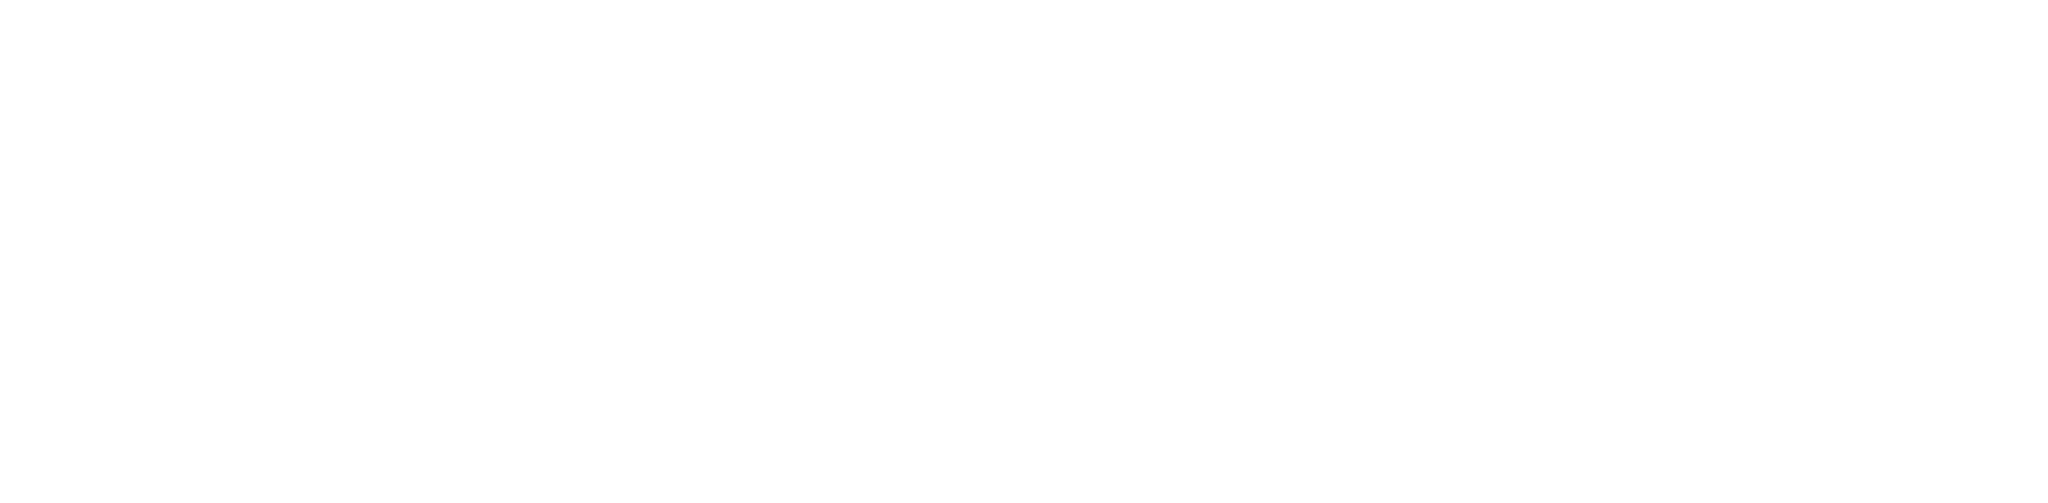
\includegraphics[trim={0 7cm 0cm 0cm},clip]{study-addressee-vp57-elan.png}
          };
         \end{tikzpicture}
       }
      \begin{footnotesize}
        \textbf{307} observations of successful communication attempts in \textbf{16} variables \vspace{10pt}
      \\\textcolor{mypurple}{\textbf{Addressee [Ar]}} \hspace{2pt} \textit{Unspecific, Parts of the Apartment, Robot, Light in the hallway  or Floor lamp}
      \pause
        \\\textcolor{myorange!50!black}{\textbf{Speech}} \hspace{2pt} Naming, Politeness, Phrasing, Sentence, Keywords
      \pause
        \\\textcolor{myyellow!50!black}{\textbf{Visual}} \hspace{2pt} FoA, Modality, Gestures, Emotions
      \pause
        \\\textcolor{mygray}{\textbf{Other}} \hspace{2pt} Id, Order, Condition, Wizard Addressee, Task
      \obcite{8-}{Holthaus2016a}
      \end{footnotesize}
\end{frame}
\begin{frame}{Addressee [Ar] Predictors}
  \begin{columns}[T] % align columns
    \begin{column}{.5\textwidth}
      \centering
      \vspace{-10pt}
      \resizebox{1.\textwidth}{!}{%
          \footnotesize
          \begin{tikzpicture}
          \action<1->{\node (a) at (0,0)
          {
            \resizebox{1.\textwidth}{!}{%
              % Created by tikzDevice version 0.12
% !TEX encoding = UTF-8 Unicode
\begin{tikzpicture}[x=1pt,y=1pt]
\definecolor{fillColor}{RGB}{255,255,255}
\path[use as bounding box,fill=fillColor,fill opacity=0.00] (0,0) rectangle (398.34,298.75);
\begin{scope}
\path[clip] ( 15.73,  0.00) rectangle (382.61,298.75);
\definecolor{drawColor}{RGB}{255,255,255}
\definecolor{fillColor}{gray}{0.98}

\path[draw=drawColor,line width= 0.6pt,line join=round,line cap=round,fill=fillColor] ( 15.73,  0.00) rectangle (382.61,298.75);
\end{scope}
\begin{scope}
\path[clip] ( 43.21, 27.47) rectangle (308.99,293.25);
\definecolor{fillColor}{gray}{0.92}

\path[fill=fillColor] ( 43.21, 27.47) rectangle (308.99,293.25);
\definecolor{drawColor}{RGB}{255,255,255}

\path[draw=drawColor,line width= 0.6pt,line join=round] ( 43.21, 37.32) --
	(308.99, 37.32);

\path[draw=drawColor,line width= 0.6pt,line join=round] ( 43.21, 53.72) --
	(308.99, 53.72);

\path[draw=drawColor,line width= 0.6pt,line join=round] ( 43.21, 70.13) --
	(308.99, 70.13);

\path[draw=drawColor,line width= 0.6pt,line join=round] ( 43.21, 86.54) --
	(308.99, 86.54);

\path[draw=drawColor,line width= 0.6pt,line join=round] ( 43.21,102.94) --
	(308.99,102.94);

\path[draw=drawColor,line width= 0.6pt,line join=round] ( 43.21,119.35) --
	(308.99,119.35);

\path[draw=drawColor,line width= 0.6pt,line join=round] ( 43.21,135.75) --
	(308.99,135.75);

\path[draw=drawColor,line width= 0.6pt,line join=round] ( 43.21,152.16) --
	(308.99,152.16);

\path[draw=drawColor,line width= 0.6pt,line join=round] ( 43.21,168.57) --
	(308.99,168.57);

\path[draw=drawColor,line width= 0.6pt,line join=round] ( 43.21,184.97) --
	(308.99,184.97);

\path[draw=drawColor,line width= 0.6pt,line join=round] ( 43.21,201.38) --
	(308.99,201.38);

\path[draw=drawColor,line width= 0.6pt,line join=round] ( 43.21,217.79) --
	(308.99,217.79);

\path[draw=drawColor,line width= 0.6pt,line join=round] ( 43.21,234.19) --
	(308.99,234.19);

\path[draw=drawColor,line width= 0.6pt,line join=round] ( 43.21,250.60) --
	(308.99,250.60);

\path[draw=drawColor,line width= 0.6pt,line join=round] ( 43.21,267.00) --
	(308.99,267.00);

\path[draw=drawColor,line width= 0.6pt,line join=round] ( 43.21,283.41) --
	(308.99,283.41);

\path[draw=drawColor,line width= 0.6pt,line join=round] ( 53.05, 27.47) --
	( 53.05,293.25);

\path[draw=drawColor,line width= 0.6pt,line join=round] ( 69.46, 27.47) --
	( 69.46,293.25);

\path[draw=drawColor,line width= 0.6pt,line join=round] ( 85.86, 27.47) --
	( 85.86,293.25);

\path[draw=drawColor,line width= 0.6pt,line join=round] (102.27, 27.47) --
	(102.27,293.25);

\path[draw=drawColor,line width= 0.6pt,line join=round] (118.67, 27.47) --
	(118.67,293.25);

\path[draw=drawColor,line width= 0.6pt,line join=round] (135.08, 27.47) --
	(135.08,293.25);

\path[draw=drawColor,line width= 0.6pt,line join=round] (151.49, 27.47) --
	(151.49,293.25);

\path[draw=drawColor,line width= 0.6pt,line join=round] (167.89, 27.47) --
	(167.89,293.25);

\path[draw=drawColor,line width= 0.6pt,line join=round] (184.30, 27.47) --
	(184.30,293.25);

\path[draw=drawColor,line width= 0.6pt,line join=round] (200.71, 27.47) --
	(200.71,293.25);

\path[draw=drawColor,line width= 0.6pt,line join=round] (217.11, 27.47) --
	(217.11,293.25);

\path[draw=drawColor,line width= 0.6pt,line join=round] (233.52, 27.47) --
	(233.52,293.25);

\path[draw=drawColor,line width= 0.6pt,line join=round] (249.92, 27.47) --
	(249.92,293.25);

\path[draw=drawColor,line width= 0.6pt,line join=round] (266.33, 27.47) --
	(266.33,293.25);

\path[draw=drawColor,line width= 0.6pt,line join=round] (282.74, 27.47) --
	(282.74,293.25);

\path[draw=drawColor,line width= 0.6pt,line join=round] (299.14, 27.47) --
	(299.14,293.25);
\definecolor{fillColor}{RGB}{5,113,176}

\path[fill=fillColor] ( 44.85, 29.11) rectangle ( 61.25, 45.52);

\path[fill=fillColor] ( 61.25, 29.11) rectangle ( 77.66, 45.52);

\path[fill=fillColor] ( 77.66, 29.11) rectangle ( 94.06, 45.52);
\definecolor{fillColor}{RGB}{244,165,130}

\path[fill=fillColor] ( 94.06, 29.11) rectangle (110.47, 45.52);
\definecolor{fillColor}{RGB}{5,113,176}

\path[fill=fillColor] (110.47, 29.11) rectangle (126.88, 45.52);

\path[fill=fillColor] (126.88, 29.11) rectangle (143.28, 45.52);

\path[fill=fillColor] (143.28, 29.11) rectangle (159.69, 45.52);

\path[fill=fillColor] (159.69, 29.11) rectangle (176.10, 45.52);

\path[fill=fillColor] (176.10, 29.11) rectangle (192.50, 45.52);

\path[fill=fillColor] (192.50, 29.11) rectangle (208.91, 45.52);

\path[fill=fillColor] (208.91, 29.11) rectangle (225.31, 45.52);

\path[fill=fillColor] (225.31, 29.11) rectangle (241.72, 45.52);

\path[fill=fillColor] (241.72, 29.11) rectangle (258.13, 45.52);
\definecolor{fillColor}{gray}{0.97}

\path[fill=fillColor] (258.13, 29.11) rectangle (274.53, 45.52);
\definecolor{fillColor}{RGB}{202,0,32}

\path[fill=fillColor] (274.53, 29.11) rectangle (290.94, 45.52);
\definecolor{fillColor}{RGB}{5,113,176}

\path[fill=fillColor] (290.94, 29.11) rectangle (307.35, 45.52);

\path[fill=fillColor] ( 44.85, 45.52) rectangle ( 61.25, 61.93);

\path[fill=fillColor] ( 61.25, 45.52) rectangle ( 77.66, 61.93);
\definecolor{fillColor}{RGB}{146,197,222}

\path[fill=fillColor] ( 77.66, 45.52) rectangle ( 94.06, 61.93);
\definecolor{fillColor}{RGB}{202,0,32}

\path[fill=fillColor] ( 94.06, 45.52) rectangle (110.47, 61.93);
\definecolor{fillColor}{RGB}{5,113,176}

\path[fill=fillColor] (110.47, 45.52) rectangle (126.88, 61.93);

\path[fill=fillColor] (126.88, 45.52) rectangle (143.28, 61.93);

\path[fill=fillColor] (143.28, 45.52) rectangle (159.69, 61.93);

\path[fill=fillColor] (159.69, 45.52) rectangle (176.10, 61.93);

\path[fill=fillColor] (176.10, 45.52) rectangle (192.50, 61.93);

\path[fill=fillColor] (192.50, 45.52) rectangle (208.91, 61.93);

\path[fill=fillColor] (208.91, 45.52) rectangle (225.31, 61.93);

\path[fill=fillColor] (225.31, 45.52) rectangle (241.72, 61.93);

\path[fill=fillColor] (241.72, 45.52) rectangle (258.13, 61.93);
\definecolor{fillColor}{gray}{0.97}

\path[fill=fillColor] (258.13, 45.52) rectangle (274.53, 61.93);

\path[fill=fillColor] (274.53, 45.52) rectangle (290.94, 61.93);
\definecolor{fillColor}{RGB}{5,113,176}

\path[fill=fillColor] (290.94, 45.52) rectangle (307.35, 61.93);

\path[fill=fillColor] ( 44.85, 61.93) rectangle ( 61.25, 78.33);
\definecolor{fillColor}{RGB}{146,197,222}

\path[fill=fillColor] ( 61.25, 61.93) rectangle ( 77.66, 78.33);
\definecolor{fillColor}{RGB}{5,113,176}

\path[fill=fillColor] ( 77.66, 61.93) rectangle ( 94.06, 78.33);
\definecolor{fillColor}{RGB}{202,0,32}

\path[fill=fillColor] ( 94.06, 61.93) rectangle (110.47, 78.33);

\path[fill=fillColor] (110.47, 61.93) rectangle (126.88, 78.33);

\path[fill=fillColor] (126.88, 61.93) rectangle (143.28, 78.33);

\path[fill=fillColor] (143.28, 61.93) rectangle (159.69, 78.33);

\path[fill=fillColor] (159.69, 61.93) rectangle (176.10, 78.33);

\path[fill=fillColor] (176.10, 61.93) rectangle (192.50, 78.33);

\path[fill=fillColor] (192.50, 61.93) rectangle (208.91, 78.33);

\path[fill=fillColor] (208.91, 61.93) rectangle (225.31, 78.33);
\definecolor{fillColor}{RGB}{244,165,130}

\path[fill=fillColor] (225.31, 61.93) rectangle (241.72, 78.33);
\definecolor{fillColor}{RGB}{202,0,32}

\path[fill=fillColor] (241.72, 61.93) rectangle (258.13, 78.33);

\path[fill=fillColor] (258.13, 61.93) rectangle (274.53, 78.33);

\path[fill=fillColor] (274.53, 61.93) rectangle (290.94, 78.33);
\definecolor{fillColor}{gray}{0.97}

\path[fill=fillColor] (290.94, 61.93) rectangle (307.35, 78.33);
\definecolor{fillColor}{RGB}{244,165,130}

\path[fill=fillColor] ( 44.85, 78.33) rectangle ( 61.25, 94.74);
\definecolor{fillColor}{RGB}{202,0,32}

\path[fill=fillColor] ( 61.25, 78.33) rectangle ( 77.66, 94.74);

\path[fill=fillColor] ( 77.66, 78.33) rectangle ( 94.06, 94.74);
\definecolor{fillColor}{RGB}{5,113,176}

\path[fill=fillColor] ( 94.06, 78.33) rectangle (110.47, 94.74);
\definecolor{fillColor}{RGB}{202,0,32}

\path[fill=fillColor] (110.47, 78.33) rectangle (126.88, 94.74);

\path[fill=fillColor] (126.88, 78.33) rectangle (143.28, 94.74);
\definecolor{fillColor}{RGB}{146,197,222}

\path[fill=fillColor] (143.28, 78.33) rectangle (159.69, 94.74);
\definecolor{fillColor}{RGB}{202,0,32}

\path[fill=fillColor] (159.69, 78.33) rectangle (176.10, 94.74);

\path[fill=fillColor] (176.10, 78.33) rectangle (192.50, 94.74);

\path[fill=fillColor] (192.50, 78.33) rectangle (208.91, 94.74);
\definecolor{fillColor}{gray}{0.97}

\path[fill=fillColor] (208.91, 78.33) rectangle (225.31, 94.74);

\path[fill=fillColor] (225.31, 78.33) rectangle (241.72, 94.74);

\path[fill=fillColor] (241.72, 78.33) rectangle (258.13, 94.74);
\definecolor{fillColor}{RGB}{202,0,32}

\path[fill=fillColor] (258.13, 78.33) rectangle (274.53, 94.74);
\definecolor{fillColor}{gray}{0.97}

\path[fill=fillColor] (274.53, 78.33) rectangle (290.94, 94.74);
\definecolor{fillColor}{RGB}{146,197,222}

\path[fill=fillColor] (290.94, 78.33) rectangle (307.35, 94.74);
\definecolor{fillColor}{RGB}{5,113,176}

\path[fill=fillColor] ( 44.85, 94.74) rectangle ( 61.25,111.15);

\path[fill=fillColor] ( 61.25, 94.74) rectangle ( 77.66,111.15);
\definecolor{fillColor}{RGB}{202,0,32}

\path[fill=fillColor] ( 77.66, 94.74) rectangle ( 94.06,111.15);

\path[fill=fillColor] ( 94.06, 94.74) rectangle (110.47,111.15);
\definecolor{fillColor}{RGB}{5,113,176}

\path[fill=fillColor] (110.47, 94.74) rectangle (126.88,111.15);

\path[fill=fillColor] (126.88, 94.74) rectangle (143.28,111.15);

\path[fill=fillColor] (143.28, 94.74) rectangle (159.69,111.15);

\path[fill=fillColor] (159.69, 94.74) rectangle (176.10,111.15);

\path[fill=fillColor] (176.10, 94.74) rectangle (192.50,111.15);

\path[fill=fillColor] (192.50, 94.74) rectangle (208.91,111.15);

\path[fill=fillColor] (208.91, 94.74) rectangle (225.31,111.15);

\path[fill=fillColor] (225.31, 94.74) rectangle (241.72,111.15);

\path[fill=fillColor] (241.72, 94.74) rectangle (258.13,111.15);
\definecolor{fillColor}{RGB}{202,0,32}

\path[fill=fillColor] (258.13, 94.74) rectangle (274.53,111.15);
\definecolor{fillColor}{RGB}{5,113,176}

\path[fill=fillColor] (274.53, 94.74) rectangle (290.94,111.15);

\path[fill=fillColor] (290.94, 94.74) rectangle (307.35,111.15);

\path[fill=fillColor] ( 44.85,111.15) rectangle ( 61.25,127.55);

\path[fill=fillColor] ( 61.25,111.15) rectangle ( 77.66,127.55);
\definecolor{fillColor}{RGB}{202,0,32}

\path[fill=fillColor] ( 77.66,111.15) rectangle ( 94.06,127.55);

\path[fill=fillColor] ( 94.06,111.15) rectangle (110.47,127.55);
\definecolor{fillColor}{RGB}{5,113,176}

\path[fill=fillColor] (110.47,111.15) rectangle (126.88,127.55);

\path[fill=fillColor] (126.88,111.15) rectangle (143.28,127.55);

\path[fill=fillColor] (143.28,111.15) rectangle (159.69,127.55);

\path[fill=fillColor] (159.69,111.15) rectangle (176.10,127.55);

\path[fill=fillColor] (176.10,111.15) rectangle (192.50,127.55);

\path[fill=fillColor] (192.50,111.15) rectangle (208.91,127.55);
\definecolor{fillColor}{RGB}{202,0,32}

\path[fill=fillColor] (208.91,111.15) rectangle (225.31,127.55);
\definecolor{fillColor}{RGB}{146,197,222}

\path[fill=fillColor] (225.31,111.15) rectangle (241.72,127.55);
\definecolor{fillColor}{gray}{0.97}

\path[fill=fillColor] (241.72,111.15) rectangle (258.13,127.55);
\definecolor{fillColor}{RGB}{202,0,32}

\path[fill=fillColor] (258.13,111.15) rectangle (274.53,127.55);
\definecolor{fillColor}{RGB}{5,113,176}

\path[fill=fillColor] (274.53,111.15) rectangle (290.94,127.55);

\path[fill=fillColor] (290.94,111.15) rectangle (307.35,127.55);

\path[fill=fillColor] ( 44.85,127.55) rectangle ( 61.25,143.96);

\path[fill=fillColor] ( 61.25,127.55) rectangle ( 77.66,143.96);
\definecolor{fillColor}{RGB}{202,0,32}

\path[fill=fillColor] ( 77.66,127.55) rectangle ( 94.06,143.96);
\definecolor{fillColor}{RGB}{146,197,222}

\path[fill=fillColor] ( 94.06,127.55) rectangle (110.47,143.96);
\definecolor{fillColor}{RGB}{5,113,176}

\path[fill=fillColor] (110.47,127.55) rectangle (126.88,143.96);

\path[fill=fillColor] (126.88,127.55) rectangle (143.28,143.96);

\path[fill=fillColor] (143.28,127.55) rectangle (159.69,143.96);

\path[fill=fillColor] (159.69,127.55) rectangle (176.10,143.96);

\path[fill=fillColor] (176.10,127.55) rectangle (192.50,143.96);

\path[fill=fillColor] (192.50,127.55) rectangle (208.91,143.96);

\path[fill=fillColor] (208.91,127.55) rectangle (225.31,143.96);

\path[fill=fillColor] (225.31,127.55) rectangle (241.72,143.96);

\path[fill=fillColor] (241.72,127.55) rectangle (258.13,143.96);
\definecolor{fillColor}{RGB}{202,0,32}

\path[fill=fillColor] (258.13,127.55) rectangle (274.53,143.96);
\definecolor{fillColor}{RGB}{5,113,176}

\path[fill=fillColor] (274.53,127.55) rectangle (290.94,143.96);

\path[fill=fillColor] (290.94,127.55) rectangle (307.35,143.96);

\path[fill=fillColor] ( 44.85,143.96) rectangle ( 61.25,160.36);

\path[fill=fillColor] ( 61.25,143.96) rectangle ( 77.66,160.36);
\definecolor{fillColor}{RGB}{202,0,32}

\path[fill=fillColor] ( 77.66,143.96) rectangle ( 94.06,160.36);

\path[fill=fillColor] ( 94.06,143.96) rectangle (110.47,160.36);
\definecolor{fillColor}{RGB}{5,113,176}

\path[fill=fillColor] (110.47,143.96) rectangle (126.88,160.36);

\path[fill=fillColor] (126.88,143.96) rectangle (143.28,160.36);

\path[fill=fillColor] (143.28,143.96) rectangle (159.69,160.36);

\path[fill=fillColor] (159.69,143.96) rectangle (176.10,160.36);

\path[fill=fillColor] (176.10,143.96) rectangle (192.50,160.36);

\path[fill=fillColor] (192.50,143.96) rectangle (208.91,160.36);

\path[fill=fillColor] (208.91,143.96) rectangle (225.31,160.36);

\path[fill=fillColor] (225.31,143.96) rectangle (241.72,160.36);

\path[fill=fillColor] (241.72,143.96) rectangle (258.13,160.36);
\definecolor{fillColor}{RGB}{244,165,130}

\path[fill=fillColor] (258.13,143.96) rectangle (274.53,160.36);
\definecolor{fillColor}{RGB}{5,113,176}

\path[fill=fillColor] (274.53,143.96) rectangle (290.94,160.36);

\path[fill=fillColor] (290.94,143.96) rectangle (307.35,160.36);

\path[fill=fillColor] ( 44.85,160.36) rectangle ( 61.25,176.77);

\path[fill=fillColor] ( 61.25,160.36) rectangle ( 77.66,176.77);
\definecolor{fillColor}{RGB}{202,0,32}

\path[fill=fillColor] ( 77.66,160.36) rectangle ( 94.06,176.77);

\path[fill=fillColor] ( 94.06,160.36) rectangle (110.47,176.77);
\definecolor{fillColor}{RGB}{5,113,176}

\path[fill=fillColor] (110.47,160.36) rectangle (126.88,176.77);

\path[fill=fillColor] (126.88,160.36) rectangle (143.28,176.77);

\path[fill=fillColor] (143.28,160.36) rectangle (159.69,176.77);

\path[fill=fillColor] (159.69,160.36) rectangle (176.10,176.77);

\path[fill=fillColor] (176.10,160.36) rectangle (192.50,176.77);

\path[fill=fillColor] (192.50,160.36) rectangle (208.91,176.77);

\path[fill=fillColor] (208.91,160.36) rectangle (225.31,176.77);

\path[fill=fillColor] (225.31,160.36) rectangle (241.72,176.77);

\path[fill=fillColor] (241.72,160.36) rectangle (258.13,176.77);
\definecolor{fillColor}{RGB}{202,0,32}

\path[fill=fillColor] (258.13,160.36) rectangle (274.53,176.77);
\definecolor{fillColor}{RGB}{5,113,176}

\path[fill=fillColor] (274.53,160.36) rectangle (290.94,176.77);
\definecolor{fillColor}{RGB}{146,197,222}

\path[fill=fillColor] (290.94,160.36) rectangle (307.35,176.77);
\definecolor{fillColor}{RGB}{5,113,176}

\path[fill=fillColor] ( 44.85,176.77) rectangle ( 61.25,193.18);

\path[fill=fillColor] ( 61.25,176.77) rectangle ( 77.66,193.18);
\definecolor{fillColor}{RGB}{202,0,32}

\path[fill=fillColor] ( 77.66,176.77) rectangle ( 94.06,193.18);

\path[fill=fillColor] ( 94.06,176.77) rectangle (110.47,193.18);
\definecolor{fillColor}{RGB}{5,113,176}

\path[fill=fillColor] (110.47,176.77) rectangle (126.88,193.18);

\path[fill=fillColor] (126.88,176.77) rectangle (143.28,193.18);

\path[fill=fillColor] (143.28,176.77) rectangle (159.69,193.18);

\path[fill=fillColor] (159.69,176.77) rectangle (176.10,193.18);

\path[fill=fillColor] (176.10,176.77) rectangle (192.50,193.18);

\path[fill=fillColor] (192.50,176.77) rectangle (208.91,193.18);

\path[fill=fillColor] (208.91,176.77) rectangle (225.31,193.18);

\path[fill=fillColor] (225.31,176.77) rectangle (241.72,193.18);

\path[fill=fillColor] (241.72,176.77) rectangle (258.13,193.18);
\definecolor{fillColor}{RGB}{202,0,32}

\path[fill=fillColor] (258.13,176.77) rectangle (274.53,193.18);
\definecolor{fillColor}{RGB}{5,113,176}

\path[fill=fillColor] (274.53,176.77) rectangle (290.94,193.18);

\path[fill=fillColor] (290.94,176.77) rectangle (307.35,193.18);

\path[fill=fillColor] ( 44.85,193.18) rectangle ( 61.25,209.58);

\path[fill=fillColor] ( 61.25,193.18) rectangle ( 77.66,209.58);
\definecolor{fillColor}{RGB}{202,0,32}

\path[fill=fillColor] ( 77.66,193.18) rectangle ( 94.06,209.58);
\definecolor{fillColor}{gray}{0.97}

\path[fill=fillColor] ( 94.06,193.18) rectangle (110.47,209.58);
\definecolor{fillColor}{RGB}{5,113,176}

\path[fill=fillColor] (110.47,193.18) rectangle (126.88,209.58);
\definecolor{fillColor}{RGB}{202,0,32}

\path[fill=fillColor] (126.88,193.18) rectangle (143.28,209.58);
\definecolor{fillColor}{RGB}{5,113,176}

\path[fill=fillColor] (143.28,193.18) rectangle (159.69,209.58);

\path[fill=fillColor] (159.69,193.18) rectangle (176.10,209.58);

\path[fill=fillColor] (176.10,193.18) rectangle (192.50,209.58);

\path[fill=fillColor] (192.50,193.18) rectangle (208.91,209.58);

\path[fill=fillColor] (208.91,193.18) rectangle (225.31,209.58);

\path[fill=fillColor] (225.31,193.18) rectangle (241.72,209.58);

\path[fill=fillColor] (241.72,193.18) rectangle (258.13,209.58);
\definecolor{fillColor}{RGB}{146,197,222}

\path[fill=fillColor] (258.13,193.18) rectangle (274.53,209.58);

\path[fill=fillColor] (274.53,193.18) rectangle (290.94,209.58);
\definecolor{fillColor}{RGB}{5,113,176}

\path[fill=fillColor] (290.94,193.18) rectangle (307.35,209.58);

\path[fill=fillColor] ( 44.85,209.58) rectangle ( 61.25,225.99);

\path[fill=fillColor] ( 61.25,209.58) rectangle ( 77.66,225.99);
\definecolor{fillColor}{RGB}{244,165,130}

\path[fill=fillColor] ( 77.66,209.58) rectangle ( 94.06,225.99);
\definecolor{fillColor}{gray}{0.97}

\path[fill=fillColor] ( 94.06,209.58) rectangle (110.47,225.99);
\definecolor{fillColor}{RGB}{5,113,176}

\path[fill=fillColor] (110.47,209.58) rectangle (126.88,225.99);
\definecolor{fillColor}{RGB}{146,197,222}

\path[fill=fillColor] (126.88,209.58) rectangle (143.28,225.99);
\definecolor{fillColor}{RGB}{5,113,176}

\path[fill=fillColor] (143.28,209.58) rectangle (159.69,225.99);

\path[fill=fillColor] (159.69,209.58) rectangle (176.10,225.99);

\path[fill=fillColor] (176.10,209.58) rectangle (192.50,225.99);

\path[fill=fillColor] (192.50,209.58) rectangle (208.91,225.99);

\path[fill=fillColor] (208.91,209.58) rectangle (225.31,225.99);

\path[fill=fillColor] (225.31,209.58) rectangle (241.72,225.99);

\path[fill=fillColor] (241.72,209.58) rectangle (258.13,225.99);
\definecolor{fillColor}{RGB}{244,165,130}

\path[fill=fillColor] (258.13,209.58) rectangle (274.53,225.99);
\definecolor{fillColor}{RGB}{202,0,32}

\path[fill=fillColor] (274.53,209.58) rectangle (290.94,225.99);
\definecolor{fillColor}{RGB}{5,113,176}

\path[fill=fillColor] (290.94,209.58) rectangle (307.35,225.99);

\path[fill=fillColor] ( 44.85,225.99) rectangle ( 61.25,242.39);

\path[fill=fillColor] ( 61.25,225.99) rectangle ( 77.66,242.39);
\definecolor{fillColor}{RGB}{202,0,32}

\path[fill=fillColor] ( 77.66,225.99) rectangle ( 94.06,242.39);
\definecolor{fillColor}{gray}{0.97}

\path[fill=fillColor] ( 94.06,225.99) rectangle (110.47,242.39);
\definecolor{fillColor}{RGB}{5,113,176}

\path[fill=fillColor] (110.47,225.99) rectangle (126.88,242.39);
\definecolor{fillColor}{gray}{0.97}

\path[fill=fillColor] (126.88,225.99) rectangle (143.28,242.39);
\definecolor{fillColor}{RGB}{5,113,176}

\path[fill=fillColor] (143.28,225.99) rectangle (159.69,242.39);

\path[fill=fillColor] (159.69,225.99) rectangle (176.10,242.39);

\path[fill=fillColor] (176.10,225.99) rectangle (192.50,242.39);

\path[fill=fillColor] (192.50,225.99) rectangle (208.91,242.39);

\path[fill=fillColor] (208.91,225.99) rectangle (225.31,242.39);

\path[fill=fillColor] (225.31,225.99) rectangle (241.72,242.39);

\path[fill=fillColor] (241.72,225.99) rectangle (258.13,242.39);
\definecolor{fillColor}{RGB}{202,0,32}

\path[fill=fillColor] (258.13,225.99) rectangle (274.53,242.39);

\path[fill=fillColor] (274.53,225.99) rectangle (290.94,242.39);

\path[fill=fillColor] (290.94,225.99) rectangle (307.35,242.39);
\definecolor{fillColor}{gray}{0.97}

\path[fill=fillColor] ( 44.85,242.39) rectangle ( 61.25,258.80);

\path[fill=fillColor] ( 61.25,242.39) rectangle ( 77.66,258.80);
\definecolor{fillColor}{RGB}{202,0,32}

\path[fill=fillColor] ( 77.66,242.39) rectangle ( 94.06,258.80);

\path[fill=fillColor] ( 94.06,242.39) rectangle (110.47,258.80);

\path[fill=fillColor] (110.47,242.39) rectangle (126.88,258.80);

\path[fill=fillColor] (126.88,242.39) rectangle (143.28,258.80);

\path[fill=fillColor] (143.28,242.39) rectangle (159.69,258.80);
\definecolor{fillColor}{RGB}{244,165,130}

\path[fill=fillColor] (159.69,242.39) rectangle (176.10,258.80);
\definecolor{fillColor}{RGB}{202,0,32}

\path[fill=fillColor] (176.10,242.39) rectangle (192.50,258.80);

\path[fill=fillColor] (192.50,242.39) rectangle (208.91,258.80);
\definecolor{fillColor}{RGB}{146,197,222}

\path[fill=fillColor] (208.91,242.39) rectangle (225.31,258.80);
\definecolor{fillColor}{RGB}{244,165,130}

\path[fill=fillColor] (225.31,242.39) rectangle (241.72,258.80);
\definecolor{fillColor}{RGB}{202,0,32}

\path[fill=fillColor] (241.72,242.39) rectangle (258.13,258.80);
\definecolor{fillColor}{RGB}{5,113,176}

\path[fill=fillColor] (258.13,242.39) rectangle (274.53,258.80);
\definecolor{fillColor}{RGB}{146,197,222}

\path[fill=fillColor] (274.53,242.39) rectangle (290.94,258.80);
\definecolor{fillColor}{RGB}{5,113,176}

\path[fill=fillColor] (290.94,242.39) rectangle (307.35,258.80);
\definecolor{fillColor}{RGB}{202,0,32}

\path[fill=fillColor] ( 44.85,258.80) rectangle ( 61.25,275.21);
\definecolor{fillColor}{gray}{0.97}

\path[fill=fillColor] ( 61.25,258.80) rectangle ( 77.66,275.21);
\definecolor{fillColor}{RGB}{202,0,32}

\path[fill=fillColor] ( 77.66,258.80) rectangle ( 94.06,275.21);
\definecolor{fillColor}{gray}{0.97}

\path[fill=fillColor] ( 94.06,258.80) rectangle (110.47,275.21);
\definecolor{fillColor}{RGB}{5,113,176}

\path[fill=fillColor] (110.47,258.80) rectangle (126.88,275.21);

\path[fill=fillColor] (126.88,258.80) rectangle (143.28,275.21);

\path[fill=fillColor] (143.28,258.80) rectangle (159.69,275.21);

\path[fill=fillColor] (159.69,258.80) rectangle (176.10,275.21);

\path[fill=fillColor] (176.10,258.80) rectangle (192.50,275.21);

\path[fill=fillColor] (192.50,258.80) rectangle (208.91,275.21);
\definecolor{fillColor}{RGB}{146,197,222}

\path[fill=fillColor] (208.91,258.80) rectangle (225.31,275.21);
\definecolor{fillColor}{RGB}{202,0,32}

\path[fill=fillColor] (225.31,258.80) rectangle (241.72,275.21);

\path[fill=fillColor] (241.72,258.80) rectangle (258.13,275.21);
\definecolor{fillColor}{RGB}{146,197,222}

\path[fill=fillColor] (258.13,258.80) rectangle (274.53,275.21);
\definecolor{fillColor}{RGB}{5,113,176}

\path[fill=fillColor] (274.53,258.80) rectangle (290.94,275.21);

\path[fill=fillColor] (290.94,258.80) rectangle (307.35,275.21);

\path[fill=fillColor] ( 44.85,275.21) rectangle ( 61.25,291.61);

\path[fill=fillColor] ( 61.25,275.21) rectangle ( 77.66,291.61);
\definecolor{fillColor}{gray}{0.97}

\path[fill=fillColor] ( 77.66,275.21) rectangle ( 94.06,291.61);
\definecolor{fillColor}{RGB}{146,197,222}

\path[fill=fillColor] ( 94.06,275.21) rectangle (110.47,291.61);
\definecolor{fillColor}{RGB}{5,113,176}

\path[fill=fillColor] (110.47,275.21) rectangle (126.88,291.61);

\path[fill=fillColor] (126.88,275.21) rectangle (143.28,291.61);

\path[fill=fillColor] (143.28,275.21) rectangle (159.69,291.61);

\path[fill=fillColor] (159.69,275.21) rectangle (176.10,291.61);
\definecolor{fillColor}{RGB}{146,197,222}

\path[fill=fillColor] (176.10,275.21) rectangle (192.50,291.61);
\definecolor{fillColor}{RGB}{5,113,176}

\path[fill=fillColor] (192.50,275.21) rectangle (208.91,291.61);

\path[fill=fillColor] (208.91,275.21) rectangle (225.31,291.61);

\path[fill=fillColor] (225.31,275.21) rectangle (241.72,291.61);
\definecolor{fillColor}{RGB}{202,0,32}

\path[fill=fillColor] (241.72,275.21) rectangle (258.13,291.61);
\definecolor{fillColor}{RGB}{5,113,176}

\path[fill=fillColor] (258.13,275.21) rectangle (274.53,291.61);

\path[fill=fillColor] (274.53,275.21) rectangle (290.94,291.61);

\path[fill=fillColor] (290.94,275.21) rectangle (307.35,291.61);
\end{scope}
\begin{scope}
\path[clip] (  0.00,  0.00) rectangle (398.34,298.75);
\definecolor{drawColor}{RGB}{0,0,0}

\node[text=drawColor,anchor=base east,inner sep=0pt, outer sep=0pt, scale=  1.00] at ( 38.26, 33.87) {Ar};

\node[text=drawColor,anchor=base east,inner sep=0pt, outer sep=0pt, scale=  1.00] at ( 38.26, 50.28) {Fr};

\node[text=drawColor,anchor=base east,inner sep=0pt, outer sep=0pt, scale=  1.00] at ( 38.26, 66.69) {Aef};

\node[text=drawColor,anchor=base east,inner sep=0pt, outer sep=0pt, scale=  1.00] at ( 38.26, 83.09) {Er};

\node[text=drawColor,anchor=base east,inner sep=0pt, outer sep=0pt, scale=  1.00] at ( 38.26, 99.50) {M};

\node[text=drawColor,anchor=base east,inner sep=0pt, outer sep=0pt, scale=  1.00] at ( 38.26,115.90) {Msr};

\node[text=drawColor,anchor=base east,inner sep=0pt, outer sep=0pt, scale=  1.00] at ( 38.26,132.31) {Sf};

\node[text=drawColor,anchor=base east,inner sep=0pt, outer sep=0pt, scale=  1.00] at ( 38.26,148.72) {Sp};

\node[text=drawColor,anchor=base east,inner sep=0pt, outer sep=0pt, scale=  1.00] at ( 38.26,165.12) {Str};

\node[text=drawColor,anchor=base east,inner sep=0pt, outer sep=0pt, scale=  1.00] at ( 38.26,181.53) {Sph};

\node[text=drawColor,anchor=base east,inner sep=0pt, outer sep=0pt, scale=  1.00] at ( 38.26,197.94) {Ssr};

\node[text=drawColor,anchor=base east,inner sep=0pt, outer sep=0pt, scale=  1.00] at ( 38.26,214.34) {Aw};

\node[text=drawColor,anchor=base east,inner sep=0pt, outer sep=0pt, scale=  1.00] at ( 38.26,230.75) {T};

\node[text=drawColor,anchor=base east,inner sep=0pt, outer sep=0pt, scale=  1.00] at ( 38.26,247.15) {C};

\node[text=drawColor,anchor=base east,inner sep=0pt, outer sep=0pt, scale=  1.00] at ( 38.26,263.56) {O};

\node[text=drawColor,anchor=base east,inner sep=0pt, outer sep=0pt, scale=  1.00] at ( 38.26,279.97) {Pid};
\end{scope}
\begin{scope}
\path[clip] (  0.00,  0.00) rectangle (398.34,298.75);
\definecolor{drawColor}{gray}{0.20}

\path[draw=drawColor,line width= 0.6pt,line join=round] ( 40.46, 37.32) --
	( 43.21, 37.32);

\path[draw=drawColor,line width= 0.6pt,line join=round] ( 40.46, 53.72) --
	( 43.21, 53.72);

\path[draw=drawColor,line width= 0.6pt,line join=round] ( 40.46, 70.13) --
	( 43.21, 70.13);

\path[draw=drawColor,line width= 0.6pt,line join=round] ( 40.46, 86.54) --
	( 43.21, 86.54);

\path[draw=drawColor,line width= 0.6pt,line join=round] ( 40.46,102.94) --
	( 43.21,102.94);

\path[draw=drawColor,line width= 0.6pt,line join=round] ( 40.46,119.35) --
	( 43.21,119.35);

\path[draw=drawColor,line width= 0.6pt,line join=round] ( 40.46,135.75) --
	( 43.21,135.75);

\path[draw=drawColor,line width= 0.6pt,line join=round] ( 40.46,152.16) --
	( 43.21,152.16);

\path[draw=drawColor,line width= 0.6pt,line join=round] ( 40.46,168.57) --
	( 43.21,168.57);

\path[draw=drawColor,line width= 0.6pt,line join=round] ( 40.46,184.97) --
	( 43.21,184.97);

\path[draw=drawColor,line width= 0.6pt,line join=round] ( 40.46,201.38) --
	( 43.21,201.38);

\path[draw=drawColor,line width= 0.6pt,line join=round] ( 40.46,217.79) --
	( 43.21,217.79);

\path[draw=drawColor,line width= 0.6pt,line join=round] ( 40.46,234.19) --
	( 43.21,234.19);

\path[draw=drawColor,line width= 0.6pt,line join=round] ( 40.46,250.60) --
	( 43.21,250.60);

\path[draw=drawColor,line width= 0.6pt,line join=round] ( 40.46,267.00) --
	( 43.21,267.00);

\path[draw=drawColor,line width= 0.6pt,line join=round] ( 40.46,283.41) --
	( 43.21,283.41);
\end{scope}
\begin{scope}
\path[clip] (  0.00,  0.00) rectangle (398.34,298.75);
\definecolor{drawColor}{gray}{0.20}

\path[draw=drawColor,line width= 0.6pt,line join=round] ( 53.05, 24.72) --
	( 53.05, 27.47);

\path[draw=drawColor,line width= 0.6pt,line join=round] ( 69.46, 24.72) --
	( 69.46, 27.47);

\path[draw=drawColor,line width= 0.6pt,line join=round] ( 85.86, 24.72) --
	( 85.86, 27.47);

\path[draw=drawColor,line width= 0.6pt,line join=round] (102.27, 24.72) --
	(102.27, 27.47);

\path[draw=drawColor,line width= 0.6pt,line join=round] (118.67, 24.72) --
	(118.67, 27.47);

\path[draw=drawColor,line width= 0.6pt,line join=round] (135.08, 24.72) --
	(135.08, 27.47);

\path[draw=drawColor,line width= 0.6pt,line join=round] (151.49, 24.72) --
	(151.49, 27.47);

\path[draw=drawColor,line width= 0.6pt,line join=round] (167.89, 24.72) --
	(167.89, 27.47);

\path[draw=drawColor,line width= 0.6pt,line join=round] (184.30, 24.72) --
	(184.30, 27.47);

\path[draw=drawColor,line width= 0.6pt,line join=round] (200.71, 24.72) --
	(200.71, 27.47);

\path[draw=drawColor,line width= 0.6pt,line join=round] (217.11, 24.72) --
	(217.11, 27.47);

\path[draw=drawColor,line width= 0.6pt,line join=round] (233.52, 24.72) --
	(233.52, 27.47);

\path[draw=drawColor,line width= 0.6pt,line join=round] (249.92, 24.72) --
	(249.92, 27.47);

\path[draw=drawColor,line width= 0.6pt,line join=round] (266.33, 24.72) --
	(266.33, 27.47);

\path[draw=drawColor,line width= 0.6pt,line join=round] (282.74, 24.72) --
	(282.74, 27.47);

\path[draw=drawColor,line width= 0.6pt,line join=round] (299.14, 24.72) --
	(299.14, 27.47);
\end{scope}
\begin{scope}
\path[clip] (  0.00,  0.00) rectangle (398.34,298.75);
\definecolor{drawColor}{RGB}{0,0,0}

\node[text=drawColor,rotate= 90.00,anchor=base east,inner sep=0pt, outer sep=0pt, scale=  1.00] at ( 59.94, 22.52) {Ar};

\node[text=drawColor,rotate= 90.00,anchor=base east,inner sep=0pt, outer sep=0pt, scale=  1.00] at ( 76.34, 22.52) {Fr};

\node[text=drawColor,rotate= 90.00,anchor=base east,inner sep=0pt, outer sep=0pt, scale=  1.00] at ( 92.75, 22.52) {Aef};

\node[text=drawColor,rotate= 90.00,anchor=base east,inner sep=0pt, outer sep=0pt, scale=  1.00] at (109.16, 22.52) {Er};

\node[text=drawColor,rotate= 90.00,anchor=base east,inner sep=0pt, outer sep=0pt, scale=  1.00] at (125.56, 22.52) {M};

\node[text=drawColor,rotate= 90.00,anchor=base east,inner sep=0pt, outer sep=0pt, scale=  1.00] at (141.97, 22.52) {Msr};

\node[text=drawColor,rotate= 90.00,anchor=base east,inner sep=0pt, outer sep=0pt, scale=  1.00] at (158.37, 22.52) {Sf};

\node[text=drawColor,rotate= 90.00,anchor=base east,inner sep=0pt, outer sep=0pt, scale=  1.00] at (174.78, 22.52) {Sp};

\node[text=drawColor,rotate= 90.00,anchor=base east,inner sep=0pt, outer sep=0pt, scale=  1.00] at (191.19, 22.52) {Str};

\node[text=drawColor,rotate= 90.00,anchor=base east,inner sep=0pt, outer sep=0pt, scale=  1.00] at (207.59, 22.52) {Sph};

\node[text=drawColor,rotate= 90.00,anchor=base east,inner sep=0pt, outer sep=0pt, scale=  1.00] at (224.00, 22.52) {Ssr};

\node[text=drawColor,rotate= 90.00,anchor=base east,inner sep=0pt, outer sep=0pt, scale=  1.00] at (240.40, 22.52) {Aw};

\node[text=drawColor,rotate= 90.00,anchor=base east,inner sep=0pt, outer sep=0pt, scale=  1.00] at (256.81, 22.52) {T};

\node[text=drawColor,rotate= 90.00,anchor=base east,inner sep=0pt, outer sep=0pt, scale=  1.00] at (273.22, 22.52) {C};

\node[text=drawColor,rotate= 90.00,anchor=base east,inner sep=0pt, outer sep=0pt, scale=  1.00] at (289.62, 22.52) {O};

\node[text=drawColor,rotate= 90.00,anchor=base east,inner sep=0pt, outer sep=0pt, scale=  1.00] at (306.03, 22.52) {Pid};
\end{scope}
\begin{scope}
\path[clip] (  0.00,  0.00) rectangle (398.34,298.75);
\definecolor{fillColor}{RGB}{255,255,255}

\path[fill=fillColor] (319.99,111.81) rectangle (377.11,208.91);
\end{scope}
\begin{scope}
\path[clip] (  0.00,  0.00) rectangle (398.34,298.75);
\definecolor{drawColor}{RGB}{0,0,0}

\node[text=drawColor,anchor=base west,inner sep=0pt, outer sep=0pt, scale=  1.00] at (325.49,195.56) {Sign. level};
\end{scope}
\begin{scope}
\path[clip] (  0.00,  0.00) rectangle (398.34,298.75);
\definecolor{drawColor}{RGB}{255,255,255}
\definecolor{fillColor}{gray}{0.95}

\path[draw=drawColor,line width= 0.6pt,line join=round,line cap=round,fill=fillColor] (325.49,175.13) rectangle (339.94,189.58);
\end{scope}
\begin{scope}
\path[clip] (  0.00,  0.00) rectangle (398.34,298.75);
\definecolor{fillColor}{RGB}{202,0,32}

\path[fill=fillColor] (325.63,175.27) rectangle (339.80,189.44);
\end{scope}
\begin{scope}
\path[clip] (  0.00,  0.00) rectangle (398.34,298.75);
\definecolor{drawColor}{RGB}{255,255,255}
\definecolor{fillColor}{gray}{0.95}

\path[draw=drawColor,line width= 0.6pt,line join=round,line cap=round,fill=fillColor] (325.49,160.68) rectangle (339.94,175.13);
\end{scope}
\begin{scope}
\path[clip] (  0.00,  0.00) rectangle (398.34,298.75);
\definecolor{fillColor}{RGB}{244,165,130}

\path[fill=fillColor] (325.63,160.82) rectangle (339.80,174.99);
\end{scope}
\begin{scope}
\path[clip] (  0.00,  0.00) rectangle (398.34,298.75);
\definecolor{drawColor}{RGB}{255,255,255}
\definecolor{fillColor}{gray}{0.95}

\path[draw=drawColor,line width= 0.6pt,line join=round,line cap=round,fill=fillColor] (325.49,146.22) rectangle (339.94,160.68);
\end{scope}
\begin{scope}
\path[clip] (  0.00,  0.00) rectangle (398.34,298.75);
\definecolor{fillColor}{gray}{0.97}

\path[fill=fillColor] (325.63,146.36) rectangle (339.80,160.53);
\end{scope}
\begin{scope}
\path[clip] (  0.00,  0.00) rectangle (398.34,298.75);
\definecolor{drawColor}{RGB}{255,255,255}
\definecolor{fillColor}{gray}{0.95}

\path[draw=drawColor,line width= 0.6pt,line join=round,line cap=round,fill=fillColor] (325.49,131.77) rectangle (339.94,146.22);
\end{scope}
\begin{scope}
\path[clip] (  0.00,  0.00) rectangle (398.34,298.75);
\definecolor{fillColor}{RGB}{146,197,222}

\path[fill=fillColor] (325.63,131.91) rectangle (339.80,146.08);
\end{scope}
\begin{scope}
\path[clip] (  0.00,  0.00) rectangle (398.34,298.75);
\definecolor{drawColor}{RGB}{255,255,255}
\definecolor{fillColor}{gray}{0.95}

\path[draw=drawColor,line width= 0.6pt,line join=round,line cap=round,fill=fillColor] (325.49,117.31) rectangle (339.94,131.77);
\end{scope}
\begin{scope}
\path[clip] (  0.00,  0.00) rectangle (398.34,298.75);
\definecolor{fillColor}{RGB}{5,113,176}

\path[fill=fillColor] (325.63,117.46) rectangle (339.80,131.62);
\end{scope}
\begin{scope}
\path[clip] (  0.00,  0.00) rectangle (398.34,298.75);
\definecolor{drawColor}{RGB}{0,0,0}

\node[text=drawColor,anchor=base west,inner sep=0pt, outer sep=0pt, scale=  0.80] at (344.94,179.60) {\( \leq 1\)};
\end{scope}
\begin{scope}
\path[clip] (  0.00,  0.00) rectangle (398.34,298.75);
\definecolor{drawColor}{RGB}{0,0,0}

\node[text=drawColor,anchor=base west,inner sep=0pt, outer sep=0pt, scale=  0.80] at (344.94,165.15) {\(< 0.1\)};
\end{scope}
\begin{scope}
\path[clip] (  0.00,  0.00) rectangle (398.34,298.75);
\definecolor{drawColor}{RGB}{0,0,0}

\node[text=drawColor,anchor=base west,inner sep=0pt, outer sep=0pt, scale=  0.80] at (344.94,150.69) {\(< 0.05\)};
\end{scope}
\begin{scope}
\path[clip] (  0.00,  0.00) rectangle (398.34,298.75);
\definecolor{drawColor}{RGB}{0,0,0}

\node[text=drawColor,anchor=base west,inner sep=0pt, outer sep=0pt, scale=  0.80] at (344.94,136.24) {\(< 0.01\)};
\end{scope}
\begin{scope}
\path[clip] (  0.00,  0.00) rectangle (398.34,298.75);
\definecolor{drawColor}{RGB}{0,0,0}

\node[text=drawColor,anchor=base west,inner sep=0pt, outer sep=0pt, scale=  0.80] at (344.94,121.79) {\(< 0.001\)};
\end{scope}
\end{tikzpicture}

            }
          };}
          \action<2->{\node (a) at (.6pt,0)
          {
            \resizebox{1.\textwidth}{!}{%
              % Created by tikzDevice version 0.12
% !TEX encoding = UTF-8 Unicode
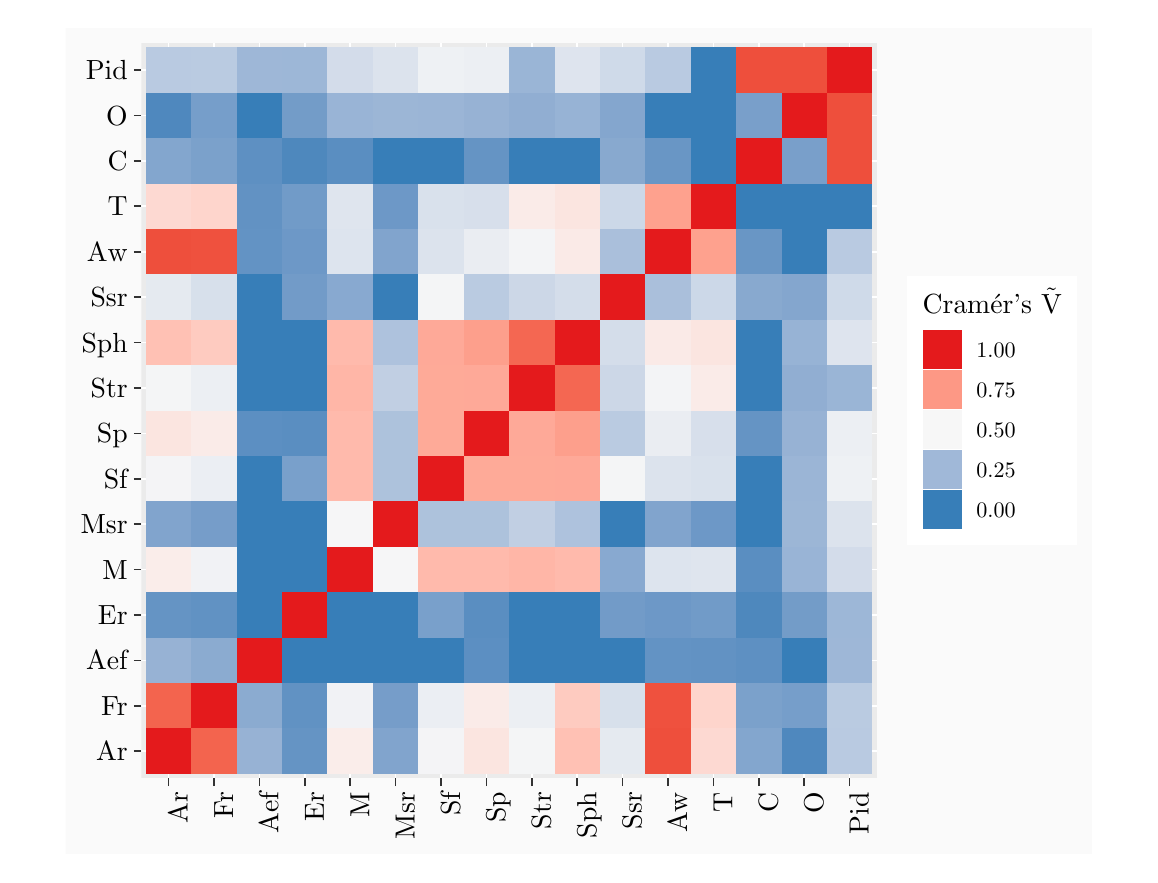
\begin{tikzpicture}[x=1pt,y=1pt]
\definecolor{fillColor}{RGB}{255,255,255}
\path[use as bounding box,fill=fillColor,fill opacity=0.00] (0,0) rectangle (398.34,298.75);
\begin{scope}
\path[clip] ( 13.60,  0.00) rectangle (384.73,298.75);
\definecolor{drawColor}{RGB}{255,255,255}
\definecolor{fillColor}{gray}{0.98}

\path[draw=drawColor,line width= 0.6pt,line join=round,line cap=round,fill=fillColor] ( 13.60,  0.00) rectangle (384.73,298.75);
\end{scope}
\begin{scope}
\path[clip] ( 41.08, 27.47) rectangle (306.86,293.25);
\definecolor{fillColor}{gray}{0.92}

\path[fill=fillColor] ( 41.08, 27.47) rectangle (306.86,293.25);
\definecolor{drawColor}{RGB}{255,255,255}

\path[draw=drawColor,line width= 0.6pt,line join=round] ( 41.08, 37.32) --
	(306.86, 37.32);

\path[draw=drawColor,line width= 0.6pt,line join=round] ( 41.08, 53.72) --
	(306.86, 53.72);

\path[draw=drawColor,line width= 0.6pt,line join=round] ( 41.08, 70.13) --
	(306.86, 70.13);

\path[draw=drawColor,line width= 0.6pt,line join=round] ( 41.08, 86.54) --
	(306.86, 86.54);

\path[draw=drawColor,line width= 0.6pt,line join=round] ( 41.08,102.94) --
	(306.86,102.94);

\path[draw=drawColor,line width= 0.6pt,line join=round] ( 41.08,119.35) --
	(306.86,119.35);

\path[draw=drawColor,line width= 0.6pt,line join=round] ( 41.08,135.75) --
	(306.86,135.75);

\path[draw=drawColor,line width= 0.6pt,line join=round] ( 41.08,152.16) --
	(306.86,152.16);

\path[draw=drawColor,line width= 0.6pt,line join=round] ( 41.08,168.57) --
	(306.86,168.57);

\path[draw=drawColor,line width= 0.6pt,line join=round] ( 41.08,184.97) --
	(306.86,184.97);

\path[draw=drawColor,line width= 0.6pt,line join=round] ( 41.08,201.38) --
	(306.86,201.38);

\path[draw=drawColor,line width= 0.6pt,line join=round] ( 41.08,217.79) --
	(306.86,217.79);

\path[draw=drawColor,line width= 0.6pt,line join=round] ( 41.08,234.19) --
	(306.86,234.19);

\path[draw=drawColor,line width= 0.6pt,line join=round] ( 41.08,250.60) --
	(306.86,250.60);

\path[draw=drawColor,line width= 0.6pt,line join=round] ( 41.08,267.00) --
	(306.86,267.00);

\path[draw=drawColor,line width= 0.6pt,line join=round] ( 41.08,283.41) --
	(306.86,283.41);

\path[draw=drawColor,line width= 0.6pt,line join=round] ( 50.92, 27.47) --
	( 50.92,293.25);

\path[draw=drawColor,line width= 0.6pt,line join=round] ( 67.33, 27.47) --
	( 67.33,293.25);

\path[draw=drawColor,line width= 0.6pt,line join=round] ( 83.73, 27.47) --
	( 83.73,293.25);

\path[draw=drawColor,line width= 0.6pt,line join=round] (100.14, 27.47) --
	(100.14,293.25);

\path[draw=drawColor,line width= 0.6pt,line join=round] (116.55, 27.47) --
	(116.55,293.25);

\path[draw=drawColor,line width= 0.6pt,line join=round] (132.95, 27.47) --
	(132.95,293.25);

\path[draw=drawColor,line width= 0.6pt,line join=round] (149.36, 27.47) --
	(149.36,293.25);

\path[draw=drawColor,line width= 0.6pt,line join=round] (165.76, 27.47) --
	(165.76,293.25);

\path[draw=drawColor,line width= 0.6pt,line join=round] (182.17, 27.47) --
	(182.17,293.25);

\path[draw=drawColor,line width= 0.6pt,line join=round] (198.58, 27.47) --
	(198.58,293.25);

\path[draw=drawColor,line width= 0.6pt,line join=round] (214.98, 27.47) --
	(214.98,293.25);

\path[draw=drawColor,line width= 0.6pt,line join=round] (231.39, 27.47) --
	(231.39,293.25);

\path[draw=drawColor,line width= 0.6pt,line join=round] (247.80, 27.47) --
	(247.80,293.25);

\path[draw=drawColor,line width= 0.6pt,line join=round] (264.20, 27.47) --
	(264.20,293.25);

\path[draw=drawColor,line width= 0.6pt,line join=round] (280.61, 27.47) --
	(280.61,293.25);

\path[draw=drawColor,line width= 0.6pt,line join=round] (297.01, 27.47) --
	(297.01,293.25);
\definecolor{fillColor}{RGB}{228,26,28}

\path[fill=fillColor] ( 42.72, 29.11) rectangle ( 59.12, 45.52);
\definecolor{fillColor}{RGB}{243,100,78}

\path[fill=fillColor] ( 59.12, 29.11) rectangle ( 75.53, 45.52);
\definecolor{fillColor}{RGB}{151,178,212}

\path[fill=fillColor] ( 75.53, 29.11) rectangle ( 91.94, 45.52);
\definecolor{fillColor}{RGB}{101,148,196}

\path[fill=fillColor] ( 91.94, 29.11) rectangle (108.34, 45.52);
\definecolor{fillColor}{RGB}{250,237,234}

\path[fill=fillColor] (108.34, 29.11) rectangle (124.75, 45.52);
\definecolor{fillColor}{RGB}{129,164,205}

\path[fill=fillColor] (124.75, 29.11) rectangle (141.16, 45.52);
\definecolor{fillColor}{RGB}{244,244,246}

\path[fill=fillColor] (141.16, 29.11) rectangle (157.56, 45.52);
\definecolor{fillColor}{RGB}{251,229,224}

\path[fill=fillColor] (157.56, 29.11) rectangle (173.97, 45.52);
\definecolor{fillColor}{RGB}{244,245,246}

\path[fill=fillColor] (173.97, 29.11) rectangle (190.37, 45.52);
\definecolor{fillColor}{RGB}{255,193,180}

\path[fill=fillColor] (190.37, 29.11) rectangle (206.78, 45.52);
\definecolor{fillColor}{RGB}{229,234,240}

\path[fill=fillColor] (206.78, 29.11) rectangle (223.19, 45.52);
\definecolor{fillColor}{RGB}{238,79,60}

\path[fill=fillColor] (223.19, 29.11) rectangle (239.59, 45.52);
\definecolor{fillColor}{RGB}{253,217,210}

\path[fill=fillColor] (239.59, 29.11) rectangle (256.00, 45.52);
\definecolor{fillColor}{RGB}{131,166,206}

\path[fill=fillColor] (256.00, 29.11) rectangle (272.40, 45.52);
\definecolor{fillColor}{RGB}{79,136,190}

\path[fill=fillColor] (272.40, 29.11) rectangle (288.81, 45.52);
\definecolor{fillColor}{RGB}{185,202,225}

\path[fill=fillColor] (288.81, 29.11) rectangle (305.22, 45.52);
\definecolor{fillColor}{RGB}{243,100,78}

\path[fill=fillColor] ( 42.72, 45.52) rectangle ( 59.12, 61.93);
\definecolor{fillColor}{RGB}{228,26,28}

\path[fill=fillColor] ( 59.12, 45.52) rectangle ( 75.53, 61.93);
\definecolor{fillColor}{RGB}{139,171,208}

\path[fill=fillColor] ( 75.53, 45.52) rectangle ( 91.94, 61.93);
\definecolor{fillColor}{RGB}{97,146,195}

\path[fill=fillColor] ( 91.94, 45.52) rectangle (108.34, 61.93);
\definecolor{fillColor}{RGB}{241,242,245}

\path[fill=fillColor] (108.34, 45.52) rectangle (124.75, 61.93);
\definecolor{fillColor}{RGB}{118,157,201}

\path[fill=fillColor] (124.75, 45.52) rectangle (141.16, 61.93);
\definecolor{fillColor}{RGB}{235,238,243}

\path[fill=fillColor] (141.16, 45.52) rectangle (157.56, 61.93);
\definecolor{fillColor}{RGB}{250,235,232}

\path[fill=fillColor] (157.56, 45.52) rectangle (173.97, 61.93);
\definecolor{fillColor}{RGB}{236,239,243}

\path[fill=fillColor] (173.97, 45.52) rectangle (190.37, 61.93);
\definecolor{fillColor}{RGB}{254,203,192}

\path[fill=fillColor] (190.37, 45.52) rectangle (206.78, 61.93);
\definecolor{fillColor}{RGB}{215,224,235}

\path[fill=fillColor] (206.78, 45.52) rectangle (223.19, 61.93);
\definecolor{fillColor}{RGB}{239,81,62}

\path[fill=fillColor] (223.19, 45.52) rectangle (239.59, 61.93);
\definecolor{fillColor}{RGB}{254,213,204}

\path[fill=fillColor] (239.59, 45.52) rectangle (256.00, 61.93);
\definecolor{fillColor}{RGB}{123,161,203}

\path[fill=fillColor] (256.00, 45.52) rectangle (272.40, 61.93);
\definecolor{fillColor}{RGB}{118,158,202}

\path[fill=fillColor] (272.40, 45.52) rectangle (288.81, 61.93);
\definecolor{fillColor}{RGB}{186,203,225}

\path[fill=fillColor] (288.81, 45.52) rectangle (305.22, 61.93);
\definecolor{fillColor}{RGB}{151,178,212}

\path[fill=fillColor] ( 42.72, 61.93) rectangle ( 59.12, 78.33);
\definecolor{fillColor}{RGB}{139,171,208}

\path[fill=fillColor] ( 59.12, 61.93) rectangle ( 75.53, 78.33);
\definecolor{fillColor}{RGB}{228,26,28}

\path[fill=fillColor] ( 75.53, 61.93) rectangle ( 91.94, 78.33);
\definecolor{fillColor}{RGB}{55,126,184}

\path[fill=fillColor] ( 91.94, 61.93) rectangle (108.34, 78.33);

\path[fill=fillColor] (108.34, 61.93) rectangle (124.75, 78.33);

\path[fill=fillColor] (124.75, 61.93) rectangle (141.16, 78.33);

\path[fill=fillColor] (141.16, 61.93) rectangle (157.56, 78.33);
\definecolor{fillColor}{RGB}{92,143,194}

\path[fill=fillColor] (157.56, 61.93) rectangle (173.97, 78.33);
\definecolor{fillColor}{RGB}{55,126,184}

\path[fill=fillColor] (173.97, 61.93) rectangle (190.37, 78.33);

\path[fill=fillColor] (190.37, 61.93) rectangle (206.78, 78.33);

\path[fill=fillColor] (206.78, 61.93) rectangle (223.19, 78.33);
\definecolor{fillColor}{RGB}{99,147,196}

\path[fill=fillColor] (223.19, 61.93) rectangle (239.59, 78.33);
\definecolor{fillColor}{RGB}{98,146,195}

\path[fill=fillColor] (239.59, 61.93) rectangle (256.00, 78.33);
\definecolor{fillColor}{RGB}{94,144,194}

\path[fill=fillColor] (256.00, 61.93) rectangle (272.40, 78.33);
\definecolor{fillColor}{RGB}{55,126,184}

\path[fill=fillColor] (272.40, 61.93) rectangle (288.81, 78.33);
\definecolor{fillColor}{RGB}{158,183,215}

\path[fill=fillColor] (288.81, 61.93) rectangle (305.22, 78.33);
\definecolor{fillColor}{RGB}{101,148,196}

\path[fill=fillColor] ( 42.72, 78.33) rectangle ( 59.12, 94.74);
\definecolor{fillColor}{RGB}{97,146,195}

\path[fill=fillColor] ( 59.12, 78.33) rectangle ( 75.53, 94.74);
\definecolor{fillColor}{RGB}{55,126,184}

\path[fill=fillColor] ( 75.53, 78.33) rectangle ( 91.94, 94.74);
\definecolor{fillColor}{RGB}{228,26,28}

\path[fill=fillColor] ( 91.94, 78.33) rectangle (108.34, 94.74);
\definecolor{fillColor}{RGB}{55,126,184}

\path[fill=fillColor] (108.34, 78.33) rectangle (124.75, 94.74);

\path[fill=fillColor] (124.75, 78.33) rectangle (141.16, 94.74);
\definecolor{fillColor}{RGB}{121,160,203}

\path[fill=fillColor] (141.16, 78.33) rectangle (157.56, 94.74);
\definecolor{fillColor}{RGB}{90,142,193}

\path[fill=fillColor] (157.56, 78.33) rectangle (173.97, 94.74);
\definecolor{fillColor}{RGB}{55,126,184}

\path[fill=fillColor] (173.97, 78.33) rectangle (190.37, 94.74);

\path[fill=fillColor] (190.37, 78.33) rectangle (206.78, 94.74);
\definecolor{fillColor}{RGB}{114,155,200}

\path[fill=fillColor] (206.78, 78.33) rectangle (223.19, 94.74);
\definecolor{fillColor}{RGB}{109,152,199}

\path[fill=fillColor] (223.19, 78.33) rectangle (239.59, 94.74);
\definecolor{fillColor}{RGB}{113,155,200}

\path[fill=fillColor] (239.59, 78.33) rectangle (256.00, 94.74);
\definecolor{fillColor}{RGB}{78,136,189}

\path[fill=fillColor] (256.00, 78.33) rectangle (272.40, 94.74);
\definecolor{fillColor}{RGB}{115,156,200}

\path[fill=fillColor] (272.40, 78.33) rectangle (288.81, 94.74);
\definecolor{fillColor}{RGB}{157,183,215}

\path[fill=fillColor] (288.81, 78.33) rectangle (305.22, 94.74);
\definecolor{fillColor}{RGB}{250,237,234}

\path[fill=fillColor] ( 42.72, 94.74) rectangle ( 59.12,111.15);
\definecolor{fillColor}{RGB}{241,242,245}

\path[fill=fillColor] ( 59.12, 94.74) rectangle ( 75.53,111.15);
\definecolor{fillColor}{RGB}{55,126,184}

\path[fill=fillColor] ( 75.53, 94.74) rectangle ( 91.94,111.15);

\path[fill=fillColor] ( 91.94, 94.74) rectangle (108.34,111.15);
\definecolor{fillColor}{RGB}{228,26,28}

\path[fill=fillColor] (108.34, 94.74) rectangle (124.75,111.15);
\definecolor{fillColor}{RGB}{246,246,247}

\path[fill=fillColor] (124.75, 94.74) rectangle (141.16,111.15);
\definecolor{fillColor}{RGB}{255,186,172}

\path[fill=fillColor] (141.16, 94.74) rectangle (157.56,111.15);

\path[fill=fillColor] (157.56, 94.74) rectangle (173.97,111.15);
\definecolor{fillColor}{RGB}{255,182,167}

\path[fill=fillColor] (173.97, 94.74) rectangle (190.37,111.15);
\definecolor{fillColor}{RGB}{255,186,172}

\path[fill=fillColor] (190.37, 94.74) rectangle (206.78,111.15);
\definecolor{fillColor}{RGB}{136,169,208}

\path[fill=fillColor] (206.78, 94.74) rectangle (223.19,111.15);
\definecolor{fillColor}{RGB}{221,228,238}

\path[fill=fillColor] (223.19, 94.74) rectangle (239.59,111.15);
\definecolor{fillColor}{RGB}{223,229,238}

\path[fill=fillColor] (239.59, 94.74) rectangle (256.00,111.15);
\definecolor{fillColor}{RGB}{90,142,193}

\path[fill=fillColor] (256.00, 94.74) rectangle (272.40,111.15);
\definecolor{fillColor}{RGB}{153,180,214}

\path[fill=fillColor] (272.40, 94.74) rectangle (288.81,111.15);
\definecolor{fillColor}{RGB}{211,220,234}

\path[fill=fillColor] (288.81, 94.74) rectangle (305.22,111.15);
\definecolor{fillColor}{RGB}{129,164,205}

\path[fill=fillColor] ( 42.72,111.15) rectangle ( 59.12,127.55);
\definecolor{fillColor}{RGB}{118,157,201}

\path[fill=fillColor] ( 59.12,111.15) rectangle ( 75.53,127.55);
\definecolor{fillColor}{RGB}{55,126,184}

\path[fill=fillColor] ( 75.53,111.15) rectangle ( 91.94,127.55);

\path[fill=fillColor] ( 91.94,111.15) rectangle (108.34,127.55);
\definecolor{fillColor}{RGB}{246,246,247}

\path[fill=fillColor] (108.34,111.15) rectangle (124.75,127.55);
\definecolor{fillColor}{RGB}{228,26,28}

\path[fill=fillColor] (124.75,111.15) rectangle (141.16,127.55);
\definecolor{fillColor}{RGB}{173,194,220}

\path[fill=fillColor] (141.16,111.15) rectangle (157.56,127.55);

\path[fill=fillColor] (157.56,111.15) rectangle (173.97,127.55);
\definecolor{fillColor}{RGB}{193,207,227}

\path[fill=fillColor] (173.97,111.15) rectangle (190.37,127.55);
\definecolor{fillColor}{RGB}{174,194,221}

\path[fill=fillColor] (190.37,111.15) rectangle (206.78,127.55);
\definecolor{fillColor}{RGB}{55,126,184}

\path[fill=fillColor] (206.78,111.15) rectangle (223.19,127.55);
\definecolor{fillColor}{RGB}{129,164,205}

\path[fill=fillColor] (223.19,111.15) rectangle (239.59,127.55);
\definecolor{fillColor}{RGB}{109,152,199}

\path[fill=fillColor] (239.59,111.15) rectangle (256.00,127.55);
\definecolor{fillColor}{RGB}{55,126,184}

\path[fill=fillColor] (256.00,111.15) rectangle (272.40,127.55);
\definecolor{fillColor}{RGB}{156,182,214}

\path[fill=fillColor] (272.40,111.15) rectangle (288.81,127.55);
\definecolor{fillColor}{RGB}{220,227,237}

\path[fill=fillColor] (288.81,111.15) rectangle (305.22,127.55);
\definecolor{fillColor}{RGB}{244,244,246}

\path[fill=fillColor] ( 42.72,127.55) rectangle ( 59.12,143.96);
\definecolor{fillColor}{RGB}{235,238,243}

\path[fill=fillColor] ( 59.12,127.55) rectangle ( 75.53,143.96);
\definecolor{fillColor}{RGB}{55,126,184}

\path[fill=fillColor] ( 75.53,127.55) rectangle ( 91.94,143.96);
\definecolor{fillColor}{RGB}{121,160,203}

\path[fill=fillColor] ( 91.94,127.55) rectangle (108.34,143.96);
\definecolor{fillColor}{RGB}{255,186,172}

\path[fill=fillColor] (108.34,127.55) rectangle (124.75,143.96);
\definecolor{fillColor}{RGB}{173,194,220}

\path[fill=fillColor] (124.75,127.55) rectangle (141.16,143.96);
\definecolor{fillColor}{RGB}{228,26,28}

\path[fill=fillColor] (141.16,127.55) rectangle (157.56,143.96);
\definecolor{fillColor}{RGB}{254,170,152}

\path[fill=fillColor] (157.56,127.55) rectangle (173.97,143.96);

\path[fill=fillColor] (173.97,127.55) rectangle (190.37,143.96);
\definecolor{fillColor}{RGB}{254,169,152}

\path[fill=fillColor] (190.37,127.55) rectangle (206.78,143.96);
\definecolor{fillColor}{RGB}{244,245,246}

\path[fill=fillColor] (206.78,127.55) rectangle (223.19,143.96);
\definecolor{fillColor}{RGB}{220,227,237}

\path[fill=fillColor] (223.19,127.55) rectangle (239.59,143.96);
\definecolor{fillColor}{RGB}{217,225,236}

\path[fill=fillColor] (239.59,127.55) rectangle (256.00,143.96);
\definecolor{fillColor}{RGB}{55,126,184}

\path[fill=fillColor] (256.00,127.55) rectangle (272.40,143.96);
\definecolor{fillColor}{RGB}{155,181,214}

\path[fill=fillColor] (272.40,127.55) rectangle (288.81,143.96);
\definecolor{fillColor}{RGB}{238,241,244}

\path[fill=fillColor] (288.81,127.55) rectangle (305.22,143.96);
\definecolor{fillColor}{RGB}{251,229,224}

\path[fill=fillColor] ( 42.72,143.96) rectangle ( 59.12,160.36);
\definecolor{fillColor}{RGB}{250,235,232}

\path[fill=fillColor] ( 59.12,143.96) rectangle ( 75.53,160.36);
\definecolor{fillColor}{RGB}{92,143,194}

\path[fill=fillColor] ( 75.53,143.96) rectangle ( 91.94,160.36);
\definecolor{fillColor}{RGB}{90,142,193}

\path[fill=fillColor] ( 91.94,143.96) rectangle (108.34,160.36);
\definecolor{fillColor}{RGB}{255,186,172}

\path[fill=fillColor] (108.34,143.96) rectangle (124.75,160.36);
\definecolor{fillColor}{RGB}{173,194,220}

\path[fill=fillColor] (124.75,143.96) rectangle (141.16,160.36);
\definecolor{fillColor}{RGB}{254,170,152}

\path[fill=fillColor] (141.16,143.96) rectangle (157.56,160.36);
\definecolor{fillColor}{RGB}{228,26,28}

\path[fill=fillColor] (157.56,143.96) rectangle (173.97,160.36);
\definecolor{fillColor}{RGB}{254,169,152}

\path[fill=fillColor] (173.97,143.96) rectangle (190.37,160.36);
\definecolor{fillColor}{RGB}{253,159,140}

\path[fill=fillColor] (190.37,143.96) rectangle (206.78,160.36);
\definecolor{fillColor}{RGB}{186,203,225}

\path[fill=fillColor] (206.78,143.96) rectangle (223.19,160.36);
\definecolor{fillColor}{RGB}{234,237,242}

\path[fill=fillColor] (223.19,143.96) rectangle (239.59,160.36);
\definecolor{fillColor}{RGB}{215,223,235}

\path[fill=fillColor] (239.59,143.96) rectangle (256.00,160.36);
\definecolor{fillColor}{RGB}{101,148,196}

\path[fill=fillColor] (256.00,143.96) rectangle (272.40,160.36);
\definecolor{fillColor}{RGB}{151,178,212}

\path[fill=fillColor] (272.40,143.96) rectangle (288.81,160.36);
\definecolor{fillColor}{RGB}{236,239,243}

\path[fill=fillColor] (288.81,143.96) rectangle (305.22,160.36);
\definecolor{fillColor}{RGB}{244,245,246}

\path[fill=fillColor] ( 42.72,160.36) rectangle ( 59.12,176.77);
\definecolor{fillColor}{RGB}{236,239,243}

\path[fill=fillColor] ( 59.12,160.36) rectangle ( 75.53,176.77);
\definecolor{fillColor}{RGB}{55,126,184}

\path[fill=fillColor] ( 75.53,160.36) rectangle ( 91.94,176.77);

\path[fill=fillColor] ( 91.94,160.36) rectangle (108.34,176.77);
\definecolor{fillColor}{RGB}{255,182,167}

\path[fill=fillColor] (108.34,160.36) rectangle (124.75,176.77);
\definecolor{fillColor}{RGB}{193,207,227}

\path[fill=fillColor] (124.75,160.36) rectangle (141.16,176.77);
\definecolor{fillColor}{RGB}{254,170,152}

\path[fill=fillColor] (141.16,160.36) rectangle (157.56,176.77);
\definecolor{fillColor}{RGB}{254,169,152}

\path[fill=fillColor] (157.56,160.36) rectangle (173.97,176.77);
\definecolor{fillColor}{RGB}{228,26,28}

\path[fill=fillColor] (173.97,160.36) rectangle (190.37,176.77);
\definecolor{fillColor}{RGB}{244,103,82}

\path[fill=fillColor] (190.37,160.36) rectangle (206.78,176.77);
\definecolor{fillColor}{RGB}{204,215,231}

\path[fill=fillColor] (206.78,160.36) rectangle (223.19,176.77);
\definecolor{fillColor}{RGB}{243,244,246}

\path[fill=fillColor] (223.19,160.36) rectangle (239.59,176.77);
\definecolor{fillColor}{RGB}{250,235,232}

\path[fill=fillColor] (239.59,160.36) rectangle (256.00,176.77);
\definecolor{fillColor}{RGB}{55,126,184}

\path[fill=fillColor] (256.00,160.36) rectangle (272.40,176.77);
\definecolor{fillColor}{RGB}{145,174,210}

\path[fill=fillColor] (272.40,160.36) rectangle (288.81,176.77);
\definecolor{fillColor}{RGB}{154,181,214}

\path[fill=fillColor] (288.81,160.36) rectangle (305.22,176.77);
\definecolor{fillColor}{RGB}{255,193,180}

\path[fill=fillColor] ( 42.72,176.77) rectangle ( 59.12,193.18);
\definecolor{fillColor}{RGB}{254,203,192}

\path[fill=fillColor] ( 59.12,176.77) rectangle ( 75.53,193.18);
\definecolor{fillColor}{RGB}{55,126,184}

\path[fill=fillColor] ( 75.53,176.77) rectangle ( 91.94,193.18);

\path[fill=fillColor] ( 91.94,176.77) rectangle (108.34,193.18);
\definecolor{fillColor}{RGB}{255,186,172}

\path[fill=fillColor] (108.34,176.77) rectangle (124.75,193.18);
\definecolor{fillColor}{RGB}{174,194,221}

\path[fill=fillColor] (124.75,176.77) rectangle (141.16,193.18);
\definecolor{fillColor}{RGB}{254,169,152}

\path[fill=fillColor] (141.16,176.77) rectangle (157.56,193.18);
\definecolor{fillColor}{RGB}{253,159,140}

\path[fill=fillColor] (157.56,176.77) rectangle (173.97,193.18);
\definecolor{fillColor}{RGB}{244,103,82}

\path[fill=fillColor] (173.97,176.77) rectangle (190.37,193.18);
\definecolor{fillColor}{RGB}{228,26,28}

\path[fill=fillColor] (190.37,176.77) rectangle (206.78,193.18);
\definecolor{fillColor}{RGB}{212,221,234}

\path[fill=fillColor] (206.78,176.77) rectangle (223.19,193.18);
\definecolor{fillColor}{RGB}{250,234,231}

\path[fill=fillColor] (223.19,176.77) rectangle (239.59,193.18);
\definecolor{fillColor}{RGB}{251,229,224}

\path[fill=fillColor] (239.59,176.77) rectangle (256.00,193.18);
\definecolor{fillColor}{RGB}{55,126,184}

\path[fill=fillColor] (256.00,176.77) rectangle (272.40,193.18);
\definecolor{fillColor}{RGB}{151,179,213}

\path[fill=fillColor] (272.40,176.77) rectangle (288.81,193.18);
\definecolor{fillColor}{RGB}{222,228,238}

\path[fill=fillColor] (288.81,176.77) rectangle (305.22,193.18);
\definecolor{fillColor}{RGB}{229,234,240}

\path[fill=fillColor] ( 42.72,193.18) rectangle ( 59.12,209.58);
\definecolor{fillColor}{RGB}{215,224,235}

\path[fill=fillColor] ( 59.12,193.18) rectangle ( 75.53,209.58);
\definecolor{fillColor}{RGB}{55,126,184}

\path[fill=fillColor] ( 75.53,193.18) rectangle ( 91.94,209.58);
\definecolor{fillColor}{RGB}{114,155,200}

\path[fill=fillColor] ( 91.94,193.18) rectangle (108.34,209.58);
\definecolor{fillColor}{RGB}{136,169,208}

\path[fill=fillColor] (108.34,193.18) rectangle (124.75,209.58);
\definecolor{fillColor}{RGB}{55,126,184}

\path[fill=fillColor] (124.75,193.18) rectangle (141.16,209.58);
\definecolor{fillColor}{RGB}{244,245,246}

\path[fill=fillColor] (141.16,193.18) rectangle (157.56,209.58);
\definecolor{fillColor}{RGB}{186,203,225}

\path[fill=fillColor] (157.56,193.18) rectangle (173.97,209.58);
\definecolor{fillColor}{RGB}{204,215,231}

\path[fill=fillColor] (173.97,193.18) rectangle (190.37,209.58);
\definecolor{fillColor}{RGB}{212,221,234}

\path[fill=fillColor] (190.37,193.18) rectangle (206.78,209.58);
\definecolor{fillColor}{RGB}{228,26,28}

\path[fill=fillColor] (206.78,193.18) rectangle (223.19,209.58);
\definecolor{fillColor}{RGB}{170,191,219}

\path[fill=fillColor] (223.19,193.18) rectangle (239.59,209.58);
\definecolor{fillColor}{RGB}{204,216,232}

\path[fill=fillColor] (239.59,193.18) rectangle (256.00,209.58);
\definecolor{fillColor}{RGB}{136,169,207}

\path[fill=fillColor] (256.00,193.18) rectangle (272.40,209.58);
\definecolor{fillColor}{RGB}{132,166,206}

\path[fill=fillColor] (272.40,193.18) rectangle (288.81,209.58);
\definecolor{fillColor}{RGB}{207,218,233}

\path[fill=fillColor] (288.81,193.18) rectangle (305.22,209.58);
\definecolor{fillColor}{RGB}{238,79,60}

\path[fill=fillColor] ( 42.72,209.58) rectangle ( 59.12,225.99);
\definecolor{fillColor}{RGB}{239,81,62}

\path[fill=fillColor] ( 59.12,209.58) rectangle ( 75.53,225.99);
\definecolor{fillColor}{RGB}{99,147,196}

\path[fill=fillColor] ( 75.53,209.58) rectangle ( 91.94,225.99);
\definecolor{fillColor}{RGB}{109,152,199}

\path[fill=fillColor] ( 91.94,209.58) rectangle (108.34,225.99);
\definecolor{fillColor}{RGB}{221,228,238}

\path[fill=fillColor] (108.34,209.58) rectangle (124.75,225.99);
\definecolor{fillColor}{RGB}{129,164,205}

\path[fill=fillColor] (124.75,209.58) rectangle (141.16,225.99);
\definecolor{fillColor}{RGB}{220,227,237}

\path[fill=fillColor] (141.16,209.58) rectangle (157.56,225.99);
\definecolor{fillColor}{RGB}{234,237,242}

\path[fill=fillColor] (157.56,209.58) rectangle (173.97,225.99);
\definecolor{fillColor}{RGB}{243,244,246}

\path[fill=fillColor] (173.97,209.58) rectangle (190.37,225.99);
\definecolor{fillColor}{RGB}{250,234,231}

\path[fill=fillColor] (190.37,209.58) rectangle (206.78,225.99);
\definecolor{fillColor}{RGB}{170,191,219}

\path[fill=fillColor] (206.78,209.58) rectangle (223.19,225.99);
\definecolor{fillColor}{RGB}{228,26,28}

\path[fill=fillColor] (223.19,209.58) rectangle (239.59,225.99);
\definecolor{fillColor}{RGB}{254,161,142}

\path[fill=fillColor] (239.59,209.58) rectangle (256.00,225.99);
\definecolor{fillColor}{RGB}{105,150,197}

\path[fill=fillColor] (256.00,209.58) rectangle (272.40,225.99);
\definecolor{fillColor}{RGB}{55,126,184}

\path[fill=fillColor] (272.40,209.58) rectangle (288.81,225.99);
\definecolor{fillColor}{RGB}{185,202,225}

\path[fill=fillColor] (288.81,209.58) rectangle (305.22,225.99);
\definecolor{fillColor}{RGB}{253,217,210}

\path[fill=fillColor] ( 42.72,225.99) rectangle ( 59.12,242.39);
\definecolor{fillColor}{RGB}{254,213,204}

\path[fill=fillColor] ( 59.12,225.99) rectangle ( 75.53,242.39);
\definecolor{fillColor}{RGB}{98,146,195}

\path[fill=fillColor] ( 75.53,225.99) rectangle ( 91.94,242.39);
\definecolor{fillColor}{RGB}{113,155,200}

\path[fill=fillColor] ( 91.94,225.99) rectangle (108.34,242.39);
\definecolor{fillColor}{RGB}{223,229,238}

\path[fill=fillColor] (108.34,225.99) rectangle (124.75,242.39);
\definecolor{fillColor}{RGB}{109,152,199}

\path[fill=fillColor] (124.75,225.99) rectangle (141.16,242.39);
\definecolor{fillColor}{RGB}{217,225,236}

\path[fill=fillColor] (141.16,225.99) rectangle (157.56,242.39);
\definecolor{fillColor}{RGB}{215,223,235}

\path[fill=fillColor] (157.56,225.99) rectangle (173.97,242.39);
\definecolor{fillColor}{RGB}{250,235,232}

\path[fill=fillColor] (173.97,225.99) rectangle (190.37,242.39);
\definecolor{fillColor}{RGB}{251,229,224}

\path[fill=fillColor] (190.37,225.99) rectangle (206.78,242.39);
\definecolor{fillColor}{RGB}{204,216,232}

\path[fill=fillColor] (206.78,225.99) rectangle (223.19,242.39);
\definecolor{fillColor}{RGB}{254,161,142}

\path[fill=fillColor] (223.19,225.99) rectangle (239.59,242.39);
\definecolor{fillColor}{RGB}{228,26,28}

\path[fill=fillColor] (239.59,225.99) rectangle (256.00,242.39);
\definecolor{fillColor}{RGB}{55,126,184}

\path[fill=fillColor] (256.00,225.99) rectangle (272.40,242.39);

\path[fill=fillColor] (272.40,225.99) rectangle (288.81,242.39);

\path[fill=fillColor] (288.81,225.99) rectangle (305.22,242.39);
\definecolor{fillColor}{RGB}{131,166,206}

\path[fill=fillColor] ( 42.72,242.39) rectangle ( 59.12,258.80);
\definecolor{fillColor}{RGB}{123,161,203}

\path[fill=fillColor] ( 59.12,242.39) rectangle ( 75.53,258.80);
\definecolor{fillColor}{RGB}{94,144,194}

\path[fill=fillColor] ( 75.53,242.39) rectangle ( 91.94,258.80);
\definecolor{fillColor}{RGB}{78,136,189}

\path[fill=fillColor] ( 91.94,242.39) rectangle (108.34,258.80);
\definecolor{fillColor}{RGB}{90,142,193}

\path[fill=fillColor] (108.34,242.39) rectangle (124.75,258.80);
\definecolor{fillColor}{RGB}{55,126,184}

\path[fill=fillColor] (124.75,242.39) rectangle (141.16,258.80);

\path[fill=fillColor] (141.16,242.39) rectangle (157.56,258.80);
\definecolor{fillColor}{RGB}{101,148,196}

\path[fill=fillColor] (157.56,242.39) rectangle (173.97,258.80);
\definecolor{fillColor}{RGB}{55,126,184}

\path[fill=fillColor] (173.97,242.39) rectangle (190.37,258.80);

\path[fill=fillColor] (190.37,242.39) rectangle (206.78,258.80);
\definecolor{fillColor}{RGB}{136,169,207}

\path[fill=fillColor] (206.78,242.39) rectangle (223.19,258.80);
\definecolor{fillColor}{RGB}{105,150,197}

\path[fill=fillColor] (223.19,242.39) rectangle (239.59,258.80);
\definecolor{fillColor}{RGB}{55,126,184}

\path[fill=fillColor] (239.59,242.39) rectangle (256.00,258.80);
\definecolor{fillColor}{RGB}{228,26,28}

\path[fill=fillColor] (256.00,242.39) rectangle (272.40,258.80);
\definecolor{fillColor}{RGB}{121,159,202}

\path[fill=fillColor] (272.40,242.39) rectangle (288.81,258.80);
\definecolor{fillColor}{RGB}{238,79,60}

\path[fill=fillColor] (288.81,242.39) rectangle (305.22,258.80);
\definecolor{fillColor}{RGB}{79,136,190}

\path[fill=fillColor] ( 42.72,258.80) rectangle ( 59.12,275.21);
\definecolor{fillColor}{RGB}{118,158,202}

\path[fill=fillColor] ( 59.12,258.80) rectangle ( 75.53,275.21);
\definecolor{fillColor}{RGB}{55,126,184}

\path[fill=fillColor] ( 75.53,258.80) rectangle ( 91.94,275.21);
\definecolor{fillColor}{RGB}{115,156,200}

\path[fill=fillColor] ( 91.94,258.80) rectangle (108.34,275.21);
\definecolor{fillColor}{RGB}{153,180,214}

\path[fill=fillColor] (108.34,258.80) rectangle (124.75,275.21);
\definecolor{fillColor}{RGB}{156,182,214}

\path[fill=fillColor] (124.75,258.80) rectangle (141.16,275.21);
\definecolor{fillColor}{RGB}{155,181,214}

\path[fill=fillColor] (141.16,258.80) rectangle (157.56,275.21);
\definecolor{fillColor}{RGB}{151,178,212}

\path[fill=fillColor] (157.56,258.80) rectangle (173.97,275.21);
\definecolor{fillColor}{RGB}{145,174,210}

\path[fill=fillColor] (173.97,258.80) rectangle (190.37,275.21);
\definecolor{fillColor}{RGB}{151,179,213}

\path[fill=fillColor] (190.37,258.80) rectangle (206.78,275.21);
\definecolor{fillColor}{RGB}{132,166,206}

\path[fill=fillColor] (206.78,258.80) rectangle (223.19,275.21);
\definecolor{fillColor}{RGB}{55,126,184}

\path[fill=fillColor] (223.19,258.80) rectangle (239.59,275.21);

\path[fill=fillColor] (239.59,258.80) rectangle (256.00,275.21);
\definecolor{fillColor}{RGB}{121,159,202}

\path[fill=fillColor] (256.00,258.80) rectangle (272.40,275.21);
\definecolor{fillColor}{RGB}{228,26,28}

\path[fill=fillColor] (272.40,258.80) rectangle (288.81,275.21);
\definecolor{fillColor}{RGB}{238,79,60}

\path[fill=fillColor] (288.81,258.80) rectangle (305.22,275.21);
\definecolor{fillColor}{RGB}{185,202,225}

\path[fill=fillColor] ( 42.72,275.21) rectangle ( 59.12,291.61);
\definecolor{fillColor}{RGB}{186,203,225}

\path[fill=fillColor] ( 59.12,275.21) rectangle ( 75.53,291.61);
\definecolor{fillColor}{RGB}{158,183,215}

\path[fill=fillColor] ( 75.53,275.21) rectangle ( 91.94,291.61);
\definecolor{fillColor}{RGB}{157,183,215}

\path[fill=fillColor] ( 91.94,275.21) rectangle (108.34,291.61);
\definecolor{fillColor}{RGB}{211,220,234}

\path[fill=fillColor] (108.34,275.21) rectangle (124.75,291.61);
\definecolor{fillColor}{RGB}{220,227,237}

\path[fill=fillColor] (124.75,275.21) rectangle (141.16,291.61);
\definecolor{fillColor}{RGB}{238,241,244}

\path[fill=fillColor] (141.16,275.21) rectangle (157.56,291.61);
\definecolor{fillColor}{RGB}{236,239,243}

\path[fill=fillColor] (157.56,275.21) rectangle (173.97,291.61);
\definecolor{fillColor}{RGB}{154,181,214}

\path[fill=fillColor] (173.97,275.21) rectangle (190.37,291.61);
\definecolor{fillColor}{RGB}{222,228,238}

\path[fill=fillColor] (190.37,275.21) rectangle (206.78,291.61);
\definecolor{fillColor}{RGB}{207,218,233}

\path[fill=fillColor] (206.78,275.21) rectangle (223.19,291.61);
\definecolor{fillColor}{RGB}{185,202,225}

\path[fill=fillColor] (223.19,275.21) rectangle (239.59,291.61);
\definecolor{fillColor}{RGB}{55,126,184}

\path[fill=fillColor] (239.59,275.21) rectangle (256.00,291.61);
\definecolor{fillColor}{RGB}{238,79,60}

\path[fill=fillColor] (256.00,275.21) rectangle (272.40,291.61);

\path[fill=fillColor] (272.40,275.21) rectangle (288.81,291.61);
\definecolor{fillColor}{RGB}{228,26,28}

\path[fill=fillColor] (288.81,275.21) rectangle (305.22,291.61);
\end{scope}
\begin{scope}
\path[clip] (  0.00,  0.00) rectangle (398.34,298.75);
\definecolor{drawColor}{RGB}{0,0,0}

\node[text=drawColor,anchor=base east,inner sep=0pt, outer sep=0pt, scale=  1.00] at ( 36.13, 33.87) {Ar};

\node[text=drawColor,anchor=base east,inner sep=0pt, outer sep=0pt, scale=  1.00] at ( 36.13, 50.28) {Fr};

\node[text=drawColor,anchor=base east,inner sep=0pt, outer sep=0pt, scale=  1.00] at ( 36.13, 66.69) {Aef};

\node[text=drawColor,anchor=base east,inner sep=0pt, outer sep=0pt, scale=  1.00] at ( 36.13, 83.09) {Er};

\node[text=drawColor,anchor=base east,inner sep=0pt, outer sep=0pt, scale=  1.00] at ( 36.13, 99.50) {M};

\node[text=drawColor,anchor=base east,inner sep=0pt, outer sep=0pt, scale=  1.00] at ( 36.13,115.90) {Msr};

\node[text=drawColor,anchor=base east,inner sep=0pt, outer sep=0pt, scale=  1.00] at ( 36.13,132.31) {Sf};

\node[text=drawColor,anchor=base east,inner sep=0pt, outer sep=0pt, scale=  1.00] at ( 36.13,148.72) {Sp};

\node[text=drawColor,anchor=base east,inner sep=0pt, outer sep=0pt, scale=  1.00] at ( 36.13,165.12) {Str};

\node[text=drawColor,anchor=base east,inner sep=0pt, outer sep=0pt, scale=  1.00] at ( 36.13,181.53) {Sph};

\node[text=drawColor,anchor=base east,inner sep=0pt, outer sep=0pt, scale=  1.00] at ( 36.13,197.94) {Ssr};

\node[text=drawColor,anchor=base east,inner sep=0pt, outer sep=0pt, scale=  1.00] at ( 36.13,214.34) {Aw};

\node[text=drawColor,anchor=base east,inner sep=0pt, outer sep=0pt, scale=  1.00] at ( 36.13,230.75) {T};

\node[text=drawColor,anchor=base east,inner sep=0pt, outer sep=0pt, scale=  1.00] at ( 36.13,247.15) {C};

\node[text=drawColor,anchor=base east,inner sep=0pt, outer sep=0pt, scale=  1.00] at ( 36.13,263.56) {O};

\node[text=drawColor,anchor=base east,inner sep=0pt, outer sep=0pt, scale=  1.00] at ( 36.13,279.97) {Pid};
\end{scope}
\begin{scope}
\path[clip] (  0.00,  0.00) rectangle (398.34,298.75);
\definecolor{drawColor}{gray}{0.20}

\path[draw=drawColor,line width= 0.6pt,line join=round] ( 38.33, 37.32) --
	( 41.08, 37.32);

\path[draw=drawColor,line width= 0.6pt,line join=round] ( 38.33, 53.72) --
	( 41.08, 53.72);

\path[draw=drawColor,line width= 0.6pt,line join=round] ( 38.33, 70.13) --
	( 41.08, 70.13);

\path[draw=drawColor,line width= 0.6pt,line join=round] ( 38.33, 86.54) --
	( 41.08, 86.54);

\path[draw=drawColor,line width= 0.6pt,line join=round] ( 38.33,102.94) --
	( 41.08,102.94);

\path[draw=drawColor,line width= 0.6pt,line join=round] ( 38.33,119.35) --
	( 41.08,119.35);

\path[draw=drawColor,line width= 0.6pt,line join=round] ( 38.33,135.75) --
	( 41.08,135.75);

\path[draw=drawColor,line width= 0.6pt,line join=round] ( 38.33,152.16) --
	( 41.08,152.16);

\path[draw=drawColor,line width= 0.6pt,line join=round] ( 38.33,168.57) --
	( 41.08,168.57);

\path[draw=drawColor,line width= 0.6pt,line join=round] ( 38.33,184.97) --
	( 41.08,184.97);

\path[draw=drawColor,line width= 0.6pt,line join=round] ( 38.33,201.38) --
	( 41.08,201.38);

\path[draw=drawColor,line width= 0.6pt,line join=round] ( 38.33,217.79) --
	( 41.08,217.79);

\path[draw=drawColor,line width= 0.6pt,line join=round] ( 38.33,234.19) --
	( 41.08,234.19);

\path[draw=drawColor,line width= 0.6pt,line join=round] ( 38.33,250.60) --
	( 41.08,250.60);

\path[draw=drawColor,line width= 0.6pt,line join=round] ( 38.33,267.00) --
	( 41.08,267.00);

\path[draw=drawColor,line width= 0.6pt,line join=round] ( 38.33,283.41) --
	( 41.08,283.41);
\end{scope}
\begin{scope}
\path[clip] (  0.00,  0.00) rectangle (398.34,298.75);
\definecolor{drawColor}{gray}{0.20}

\path[draw=drawColor,line width= 0.6pt,line join=round] ( 50.92, 24.72) --
	( 50.92, 27.47);

\path[draw=drawColor,line width= 0.6pt,line join=round] ( 67.33, 24.72) --
	( 67.33, 27.47);

\path[draw=drawColor,line width= 0.6pt,line join=round] ( 83.73, 24.72) --
	( 83.73, 27.47);

\path[draw=drawColor,line width= 0.6pt,line join=round] (100.14, 24.72) --
	(100.14, 27.47);

\path[draw=drawColor,line width= 0.6pt,line join=round] (116.55, 24.72) --
	(116.55, 27.47);

\path[draw=drawColor,line width= 0.6pt,line join=round] (132.95, 24.72) --
	(132.95, 27.47);

\path[draw=drawColor,line width= 0.6pt,line join=round] (149.36, 24.72) --
	(149.36, 27.47);

\path[draw=drawColor,line width= 0.6pt,line join=round] (165.76, 24.72) --
	(165.76, 27.47);

\path[draw=drawColor,line width= 0.6pt,line join=round] (182.17, 24.72) --
	(182.17, 27.47);

\path[draw=drawColor,line width= 0.6pt,line join=round] (198.58, 24.72) --
	(198.58, 27.47);

\path[draw=drawColor,line width= 0.6pt,line join=round] (214.98, 24.72) --
	(214.98, 27.47);

\path[draw=drawColor,line width= 0.6pt,line join=round] (231.39, 24.72) --
	(231.39, 27.47);

\path[draw=drawColor,line width= 0.6pt,line join=round] (247.80, 24.72) --
	(247.80, 27.47);

\path[draw=drawColor,line width= 0.6pt,line join=round] (264.20, 24.72) --
	(264.20, 27.47);

\path[draw=drawColor,line width= 0.6pt,line join=round] (280.61, 24.72) --
	(280.61, 27.47);

\path[draw=drawColor,line width= 0.6pt,line join=round] (297.01, 24.72) --
	(297.01, 27.47);
\end{scope}
\begin{scope}
\path[clip] (  0.00,  0.00) rectangle (398.34,298.75);
\definecolor{drawColor}{RGB}{0,0,0}

\node[text=drawColor,rotate= 90.00,anchor=base east,inner sep=0pt, outer sep=0pt, scale=  1.00] at ( 57.81, 22.52) {Ar};

\node[text=drawColor,rotate= 90.00,anchor=base east,inner sep=0pt, outer sep=0pt, scale=  1.00] at ( 74.21, 22.52) {Fr};

\node[text=drawColor,rotate= 90.00,anchor=base east,inner sep=0pt, outer sep=0pt, scale=  1.00] at ( 90.62, 22.52) {Aef};

\node[text=drawColor,rotate= 90.00,anchor=base east,inner sep=0pt, outer sep=0pt, scale=  1.00] at (107.03, 22.52) {Er};

\node[text=drawColor,rotate= 90.00,anchor=base east,inner sep=0pt, outer sep=0pt, scale=  1.00] at (123.43, 22.52) {M};

\node[text=drawColor,rotate= 90.00,anchor=base east,inner sep=0pt, outer sep=0pt, scale=  1.00] at (139.84, 22.52) {Msr};

\node[text=drawColor,rotate= 90.00,anchor=base east,inner sep=0pt, outer sep=0pt, scale=  1.00] at (156.25, 22.52) {Sf};

\node[text=drawColor,rotate= 90.00,anchor=base east,inner sep=0pt, outer sep=0pt, scale=  1.00] at (172.65, 22.52) {Sp};

\node[text=drawColor,rotate= 90.00,anchor=base east,inner sep=0pt, outer sep=0pt, scale=  1.00] at (189.06, 22.52) {Str};

\node[text=drawColor,rotate= 90.00,anchor=base east,inner sep=0pt, outer sep=0pt, scale=  1.00] at (205.46, 22.52) {Sph};

\node[text=drawColor,rotate= 90.00,anchor=base east,inner sep=0pt, outer sep=0pt, scale=  1.00] at (221.87, 22.52) {Ssr};

\node[text=drawColor,rotate= 90.00,anchor=base east,inner sep=0pt, outer sep=0pt, scale=  1.00] at (238.28, 22.52) {Aw};

\node[text=drawColor,rotate= 90.00,anchor=base east,inner sep=0pt, outer sep=0pt, scale=  1.00] at (254.68, 22.52) {T};

\node[text=drawColor,rotate= 90.00,anchor=base east,inner sep=0pt, outer sep=0pt, scale=  1.00] at (271.09, 22.52) {C};

\node[text=drawColor,rotate= 90.00,anchor=base east,inner sep=0pt, outer sep=0pt, scale=  1.00] at (287.50, 22.52) {O};

\node[text=drawColor,rotate= 90.00,anchor=base east,inner sep=0pt, outer sep=0pt, scale=  1.00] at (303.90, 22.52) {Pid};
\end{scope}
\begin{scope}
\path[clip] (  0.00,  0.00) rectangle (398.34,298.75);
\definecolor{fillColor}{RGB}{255,255,255}

\path[fill=fillColor] (317.86,111.81) rectangle (379.23,208.91);
\end{scope}
\begin{scope}
\path[clip] (  0.00,  0.00) rectangle (398.34,298.75);
\definecolor{drawColor}{RGB}{0,0,0}

\node[text=drawColor,anchor=base west,inner sep=0pt, outer sep=0pt, scale=  1.00] at (323.36,195.56) {Cram\'er's \~V};
\end{scope}
\begin{scope}
\path[clip] (  0.00,  0.00) rectangle (398.34,298.75);
\definecolor{drawColor}{RGB}{255,255,255}
\definecolor{fillColor}{gray}{0.95}

\path[draw=drawColor,line width= 0.6pt,line join=round,line cap=round,fill=fillColor] (323.36,175.13) rectangle (337.81,189.58);
\end{scope}
\begin{scope}
\path[clip] (  0.00,  0.00) rectangle (398.34,298.75);
\definecolor{fillColor}{RGB}{228,26,28}

\path[fill=fillColor] (323.50,175.27) rectangle (337.67,189.44);
\end{scope}
\begin{scope}
\path[clip] (  0.00,  0.00) rectangle (398.34,298.75);
\definecolor{drawColor}{RGB}{255,255,255}
\definecolor{fillColor}{gray}{0.95}

\path[draw=drawColor,line width= 0.6pt,line join=round,line cap=round,fill=fillColor] (323.36,160.68) rectangle (337.81,175.13);
\end{scope}
\begin{scope}
\path[clip] (  0.00,  0.00) rectangle (398.34,298.75);
\definecolor{fillColor}{RGB}{253,152,133}

\path[fill=fillColor] (323.50,160.82) rectangle (337.67,174.99);
\end{scope}
\begin{scope}
\path[clip] (  0.00,  0.00) rectangle (398.34,298.75);
\definecolor{drawColor}{RGB}{255,255,255}
\definecolor{fillColor}{gray}{0.95}

\path[draw=drawColor,line width= 0.6pt,line join=round,line cap=round,fill=fillColor] (323.36,146.22) rectangle (337.81,160.68);
\end{scope}
\begin{scope}
\path[clip] (  0.00,  0.00) rectangle (398.34,298.75);
\definecolor{fillColor}{gray}{0.97}

\path[fill=fillColor] (323.50,146.36) rectangle (337.67,160.53);
\end{scope}
\begin{scope}
\path[clip] (  0.00,  0.00) rectangle (398.34,298.75);
\definecolor{drawColor}{RGB}{255,255,255}
\definecolor{fillColor}{gray}{0.95}

\path[draw=drawColor,line width= 0.6pt,line join=round,line cap=round,fill=fillColor] (323.36,131.77) rectangle (337.81,146.22);
\end{scope}
\begin{scope}
\path[clip] (  0.00,  0.00) rectangle (398.34,298.75);
\definecolor{fillColor}{RGB}{160,184,216}

\path[fill=fillColor] (323.50,131.91) rectangle (337.67,146.08);
\end{scope}
\begin{scope}
\path[clip] (  0.00,  0.00) rectangle (398.34,298.75);
\definecolor{drawColor}{RGB}{255,255,255}
\definecolor{fillColor}{gray}{0.95}

\path[draw=drawColor,line width= 0.6pt,line join=round,line cap=round,fill=fillColor] (323.36,117.31) rectangle (337.81,131.77);
\end{scope}
\begin{scope}
\path[clip] (  0.00,  0.00) rectangle (398.34,298.75);
\definecolor{fillColor}{RGB}{55,126,184}

\path[fill=fillColor] (323.50,117.46) rectangle (337.67,131.62);
\end{scope}
\begin{scope}
\path[clip] (  0.00,  0.00) rectangle (398.34,298.75);
\definecolor{drawColor}{RGB}{0,0,0}

\node[text=drawColor,anchor=base west,inner sep=0pt, outer sep=0pt, scale=  0.80] at (342.81,179.60) {1.00};
\end{scope}
\begin{scope}
\path[clip] (  0.00,  0.00) rectangle (398.34,298.75);
\definecolor{drawColor}{RGB}{0,0,0}

\node[text=drawColor,anchor=base west,inner sep=0pt, outer sep=0pt, scale=  0.80] at (342.81,165.15) {0.75};
\end{scope}
\begin{scope}
\path[clip] (  0.00,  0.00) rectangle (398.34,298.75);
\definecolor{drawColor}{RGB}{0,0,0}

\node[text=drawColor,anchor=base west,inner sep=0pt, outer sep=0pt, scale=  0.80] at (342.81,150.69) {0.50};
\end{scope}
\begin{scope}
\path[clip] (  0.00,  0.00) rectangle (398.34,298.75);
\definecolor{drawColor}{RGB}{0,0,0}

\node[text=drawColor,anchor=base west,inner sep=0pt, outer sep=0pt, scale=  0.80] at (342.81,136.24) {0.25};
\end{scope}
\begin{scope}
\path[clip] (  0.00,  0.00) rectangle (398.34,298.75);
\definecolor{drawColor}{RGB}{0,0,0}

\node[text=drawColor,anchor=base west,inner sep=0pt, outer sep=0pt, scale=  0.80] at (342.81,121.79) {0.00};
\end{scope}
\end{tikzpicture}

            }
          };}
          \action<4->{\node (a) at (.25\textwidth,-.55\textwidth)
          {
            \resizebox{.5\textwidth}{!}{%
              % Created by tikzDevice version 0.12
% !TEX encoding = UTF-8 Unicode
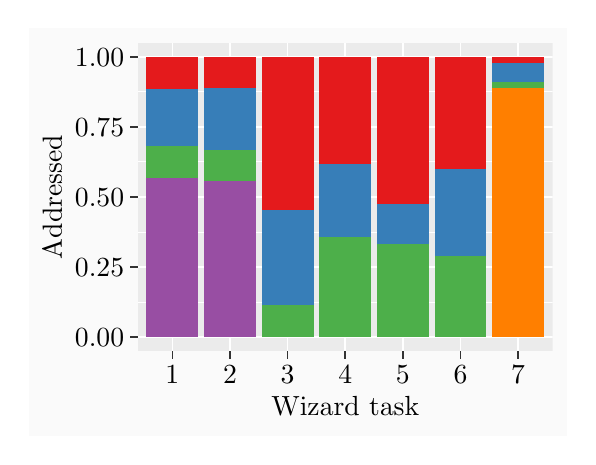
\begin{tikzpicture}[x=1pt,y=1pt]
\definecolor{fillColor}{RGB}{255,255,255}
\path[use as bounding box,fill=fillColor,fill opacity=0.00] (0,0) rectangle (195.19,147.70);
\begin{scope}
\path[clip] (  0.00,  0.00) rectangle (195.19,147.70);
\definecolor{drawColor}{RGB}{255,255,255}
\definecolor{fillColor}{gray}{0.98}

\path[draw=drawColor,line width= 0.6pt,line join=round,line cap=round,fill=fillColor] (  0.00,  0.00) rectangle (195.19,147.70);
\end{scope}
\begin{scope}
\path[clip] ( 39.80, 30.86) rectangle (189.69,142.20);
\definecolor{fillColor}{gray}{0.92}

\path[fill=fillColor] ( 39.80, 30.86) rectangle (189.69,142.20);
\definecolor{drawColor}{RGB}{255,255,255}

\path[draw=drawColor,line width= 0.3pt,line join=round] ( 39.80, 48.58) --
	(189.69, 48.58);

\path[draw=drawColor,line width= 0.3pt,line join=round] ( 39.80, 73.88) --
	(189.69, 73.88);

\path[draw=drawColor,line width= 0.3pt,line join=round] ( 39.80, 99.19) --
	(189.69, 99.19);

\path[draw=drawColor,line width= 0.3pt,line join=round] ( 39.80,124.49) --
	(189.69,124.49);

\path[draw=drawColor,line width= 0.6pt,line join=round] ( 39.80, 35.92) --
	(189.69, 35.92);

\path[draw=drawColor,line width= 0.6pt,line join=round] ( 39.80, 61.23) --
	(189.69, 61.23);

\path[draw=drawColor,line width= 0.6pt,line join=round] ( 39.80, 86.53) --
	(189.69, 86.53);

\path[draw=drawColor,line width= 0.6pt,line join=round] ( 39.80,111.84) --
	(189.69,111.84);

\path[draw=drawColor,line width= 0.6pt,line join=round] ( 39.80,137.14) --
	(189.69,137.14);

\path[draw=drawColor,line width= 0.6pt,line join=round] ( 52.29, 30.86) --
	( 52.29,142.20);

\path[draw=drawColor,line width= 0.6pt,line join=round] ( 73.11, 30.86) --
	( 73.11,142.20);

\path[draw=drawColor,line width= 0.6pt,line join=round] ( 93.93, 30.86) --
	( 93.93,142.20);

\path[draw=drawColor,line width= 0.6pt,line join=round] (114.75, 30.86) --
	(114.75,142.20);

\path[draw=drawColor,line width= 0.6pt,line join=round] (135.56, 30.86) --
	(135.56,142.20);

\path[draw=drawColor,line width= 0.6pt,line join=round] (156.38, 30.86) --
	(156.38,142.20);

\path[draw=drawColor,line width= 0.6pt,line join=round] (177.20, 30.86) --
	(177.20,142.20);
\definecolor{fillColor}{RGB}{152,78,163}

\path[fill=fillColor] ( 42.93, 35.92) rectangle ( 61.66, 93.43);
\definecolor{fillColor}{RGB}{77,175,74}

\path[fill=fillColor] ( 42.93, 93.43) rectangle ( 61.66,104.94);
\definecolor{fillColor}{RGB}{55,126,184}

\path[fill=fillColor] ( 42.93,104.94) rectangle ( 61.66,125.64);
\definecolor{fillColor}{RGB}{228,26,28}

\path[fill=fillColor] ( 42.93,125.64) rectangle ( 61.66,137.14);
\definecolor{fillColor}{RGB}{152,78,163}

\path[fill=fillColor] ( 63.74, 35.92) rectangle ( 82.48, 92.16);
\definecolor{fillColor}{RGB}{77,175,74}

\path[fill=fillColor] ( 63.74, 92.16) rectangle ( 82.48,103.40);
\definecolor{fillColor}{RGB}{55,126,184}

\path[fill=fillColor] ( 63.74,103.40) rectangle ( 82.48,125.90);
\definecolor{fillColor}{RGB}{228,26,28}

\path[fill=fillColor] ( 63.74,125.90) rectangle ( 82.48,137.14);
\definecolor{fillColor}{RGB}{77,175,74}

\path[fill=fillColor] ( 84.56, 35.92) rectangle (103.30, 47.43);
\definecolor{fillColor}{RGB}{55,126,184}

\path[fill=fillColor] ( 84.56, 47.43) rectangle (103.30, 81.93);
\definecolor{fillColor}{RGB}{228,26,28}

\path[fill=fillColor] ( 84.56, 81.93) rectangle (103.30,137.14);
\definecolor{fillColor}{RGB}{77,175,74}

\path[fill=fillColor] (105.38, 35.92) rectangle (124.11, 72.07);
\definecolor{fillColor}{RGB}{55,126,184}

\path[fill=fillColor] (105.38, 72.07) rectangle (124.11, 98.58);
\definecolor{fillColor}{RGB}{228,26,28}

\path[fill=fillColor] (105.38, 98.58) rectangle (124.11,137.14);
\definecolor{fillColor}{RGB}{77,175,74}

\path[fill=fillColor] (126.19, 35.92) rectangle (144.93, 69.66);
\definecolor{fillColor}{RGB}{55,126,184}

\path[fill=fillColor] (126.19, 69.66) rectangle (144.93, 84.12);
\definecolor{fillColor}{RGB}{228,26,28}

\path[fill=fillColor] (126.19, 84.12) rectangle (144.93,137.14);
\definecolor{fillColor}{RGB}{77,175,74}

\path[fill=fillColor] (147.01, 35.92) rectangle (165.75, 65.16);
\definecolor{fillColor}{RGB}{55,126,184}

\path[fill=fillColor] (147.01, 65.16) rectangle (165.75, 96.66);
\definecolor{fillColor}{RGB}{228,26,28}

\path[fill=fillColor] (147.01, 96.66) rectangle (165.75,137.14);
\definecolor{fillColor}{RGB}{255,127,0}

\path[fill=fillColor] (167.83, 35.92) rectangle (186.56,125.90);
\definecolor{fillColor}{RGB}{77,175,74}

\path[fill=fillColor] (167.83,125.90) rectangle (186.56,128.15);
\definecolor{fillColor}{RGB}{55,126,184}

\path[fill=fillColor] (167.83,128.15) rectangle (186.56,134.89);
\definecolor{fillColor}{RGB}{228,26,28}

\path[fill=fillColor] (167.83,134.89) rectangle (186.56,137.14);
\end{scope}
\begin{scope}
\path[clip] (  0.00,  0.00) rectangle (195.19,147.70);
\definecolor{drawColor}{RGB}{0,0,0}

\node[text=drawColor,anchor=base east,inner sep=0pt, outer sep=0pt, scale=  1.00] at ( 34.85, 32.48) {0.00};

\node[text=drawColor,anchor=base east,inner sep=0pt, outer sep=0pt, scale=  1.00] at ( 34.85, 57.78) {0.25};

\node[text=drawColor,anchor=base east,inner sep=0pt, outer sep=0pt, scale=  1.00] at ( 34.85, 83.09) {0.50};

\node[text=drawColor,anchor=base east,inner sep=0pt, outer sep=0pt, scale=  1.00] at ( 34.85,108.39) {0.75};

\node[text=drawColor,anchor=base east,inner sep=0pt, outer sep=0pt, scale=  1.00] at ( 34.85,133.70) {1.00};
\end{scope}
\begin{scope}
\path[clip] (  0.00,  0.00) rectangle (195.19,147.70);
\definecolor{drawColor}{gray}{0.20}

\path[draw=drawColor,line width= 0.6pt,line join=round] ( 37.05, 35.92) --
	( 39.80, 35.92);

\path[draw=drawColor,line width= 0.6pt,line join=round] ( 37.05, 61.23) --
	( 39.80, 61.23);

\path[draw=drawColor,line width= 0.6pt,line join=round] ( 37.05, 86.53) --
	( 39.80, 86.53);

\path[draw=drawColor,line width= 0.6pt,line join=round] ( 37.05,111.84) --
	( 39.80,111.84);

\path[draw=drawColor,line width= 0.6pt,line join=round] ( 37.05,137.14) --
	( 39.80,137.14);
\end{scope}
\begin{scope}
\path[clip] (  0.00,  0.00) rectangle (195.19,147.70);
\definecolor{drawColor}{gray}{0.20}

\path[draw=drawColor,line width= 0.6pt,line join=round] ( 52.29, 28.11) --
	( 52.29, 30.86);

\path[draw=drawColor,line width= 0.6pt,line join=round] ( 73.11, 28.11) --
	( 73.11, 30.86);

\path[draw=drawColor,line width= 0.6pt,line join=round] ( 93.93, 28.11) --
	( 93.93, 30.86);

\path[draw=drawColor,line width= 0.6pt,line join=round] (114.75, 28.11) --
	(114.75, 30.86);

\path[draw=drawColor,line width= 0.6pt,line join=round] (135.56, 28.11) --
	(135.56, 30.86);

\path[draw=drawColor,line width= 0.6pt,line join=round] (156.38, 28.11) --
	(156.38, 30.86);

\path[draw=drawColor,line width= 0.6pt,line join=round] (177.20, 28.11) --
	(177.20, 30.86);
\end{scope}
\begin{scope}
\path[clip] (  0.00,  0.00) rectangle (195.19,147.70);
\definecolor{drawColor}{RGB}{0,0,0}

\node[text=drawColor,anchor=base,inner sep=0pt, outer sep=0pt, scale=  1.00] at ( 52.29, 19.03) {1};

\node[text=drawColor,anchor=base,inner sep=0pt, outer sep=0pt, scale=  1.00] at ( 73.11, 19.03) {2};

\node[text=drawColor,anchor=base,inner sep=0pt, outer sep=0pt, scale=  1.00] at ( 93.93, 19.03) {3};

\node[text=drawColor,anchor=base,inner sep=0pt, outer sep=0pt, scale=  1.00] at (114.75, 19.03) {4};

\node[text=drawColor,anchor=base,inner sep=0pt, outer sep=0pt, scale=  1.00] at (135.56, 19.03) {5};

\node[text=drawColor,anchor=base,inner sep=0pt, outer sep=0pt, scale=  1.00] at (156.38, 19.03) {6};

\node[text=drawColor,anchor=base,inner sep=0pt, outer sep=0pt, scale=  1.00] at (177.20, 19.03) {7};
\end{scope}
\begin{scope}
\path[clip] (  0.00,  0.00) rectangle (195.19,147.70);
\definecolor{drawColor}{RGB}{0,0,0}

\node[text=drawColor,anchor=base,inner sep=0pt, outer sep=0pt, scale=  1.00] at (114.75,  7.44) {Wizard task};
\end{scope}
\begin{scope}
\path[clip] (  0.00,  0.00) rectangle (195.19,147.70);
\definecolor{drawColor}{RGB}{0,0,0}

\node[text=drawColor,rotate= 90.00,anchor=base,inner sep=0pt, outer sep=0pt, scale=  1.00] at ( 12.39, 86.53) {Addressed};
\end{scope}
\end{tikzpicture}

            }
          };}
          \action<3->{\node (a) at (-.25\textwidth,-.55\textwidth)
          {
            \resizebox{.5\textwidth}{!}{%
              % Created by tikzDevice version 0.12
% !TEX encoding = UTF-8 Unicode
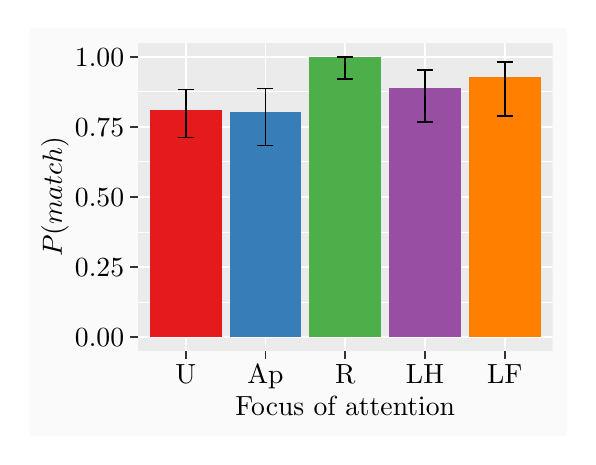
\begin{tikzpicture}[x=1pt,y=1pt]
\definecolor{fillColor}{RGB}{255,255,255}
\path[use as bounding box,fill=fillColor,fill opacity=0.00] (0,0) rectangle (195.19,147.70);
\begin{scope}
\path[clip] (  0.00,  0.00) rectangle (195.19,147.70);
\definecolor{drawColor}{RGB}{255,255,255}
\definecolor{fillColor}{gray}{0.98}

\path[draw=drawColor,line width= 0.6pt,line join=round,line cap=round,fill=fillColor] (  0.00,  0.00) rectangle (195.19,147.70);
\end{scope}
\begin{scope}
\path[clip] ( 39.80, 30.86) rectangle (189.69,142.20);
\definecolor{fillColor}{gray}{0.92}

\path[fill=fillColor] ( 39.80, 30.86) rectangle (189.69,142.20);
\definecolor{drawColor}{RGB}{255,255,255}

\path[draw=drawColor,line width= 0.3pt,line join=round] ( 39.80, 48.58) --
	(189.69, 48.58);

\path[draw=drawColor,line width= 0.3pt,line join=round] ( 39.80, 73.88) --
	(189.69, 73.88);

\path[draw=drawColor,line width= 0.3pt,line join=round] ( 39.80, 99.19) --
	(189.69, 99.19);

\path[draw=drawColor,line width= 0.3pt,line join=round] ( 39.80,124.49) --
	(189.69,124.49);

\path[draw=drawColor,line width= 0.6pt,line join=round] ( 39.80, 35.92) --
	(189.69, 35.92);

\path[draw=drawColor,line width= 0.6pt,line join=round] ( 39.80, 61.23) --
	(189.69, 61.23);

\path[draw=drawColor,line width= 0.6pt,line join=round] ( 39.80, 86.53) --
	(189.69, 86.53);

\path[draw=drawColor,line width= 0.6pt,line join=round] ( 39.80,111.84) --
	(189.69,111.84);

\path[draw=drawColor,line width= 0.6pt,line join=round] ( 39.80,137.14) --
	(189.69,137.14);

\path[draw=drawColor,line width= 0.6pt,line join=round] ( 57.10, 30.86) --
	( 57.10,142.20);

\path[draw=drawColor,line width= 0.6pt,line join=round] ( 85.92, 30.86) --
	( 85.92,142.20);

\path[draw=drawColor,line width= 0.6pt,line join=round] (114.75, 30.86) --
	(114.75,142.20);

\path[draw=drawColor,line width= 0.6pt,line join=round] (143.57, 30.86) --
	(143.57,142.20);

\path[draw=drawColor,line width= 0.6pt,line join=round] (172.39, 30.86) --
	(172.39,142.20);
\definecolor{fillColor}{RGB}{228,26,28}

\path[fill=fillColor] ( 44.13, 35.92) rectangle ( 70.07,118.02);
\definecolor{fillColor}{RGB}{55,126,184}

\path[fill=fillColor] ( 72.95, 35.92) rectangle ( 98.89,117.21);
\definecolor{fillColor}{RGB}{77,175,74}

\path[fill=fillColor] (101.77, 35.92) rectangle (127.72,137.14);
\definecolor{fillColor}{RGB}{152,78,163}

\path[fill=fillColor] (130.60, 35.92) rectangle (156.54,125.90);
\definecolor{fillColor}{RGB}{255,127,0}

\path[fill=fillColor] (159.42, 35.92) rectangle (185.36,129.74);
\definecolor{drawColor}{RGB}{0,0,0}

\path[draw=drawColor,line width= 0.6pt,line join=round] ( 54.22,125.31) --
	( 59.98,125.31);

\path[draw=drawColor,line width= 0.6pt,line join=round] ( 57.10,125.31) --
	( 57.10,107.99);

\path[draw=drawColor,line width= 0.6pt,line join=round] ( 54.22,107.99) --
	( 59.98,107.99);

\path[draw=drawColor,line width= 0.6pt,line join=round] ( 83.04,125.70) --
	( 88.80,125.70);

\path[draw=drawColor,line width= 0.6pt,line join=round] ( 85.92,125.70) --
	( 85.92,105.08);

\path[draw=drawColor,line width= 0.6pt,line join=round] ( 83.04,105.08) --
	( 88.80,105.08);

\path[draw=drawColor,line width= 0.6pt,line join=round] (111.86,137.14) --
	(117.63,137.14);

\path[draw=drawColor,line width= 0.6pt,line join=round] (114.75,137.14) --
	(114.75,129.05);

\path[draw=drawColor,line width= 0.6pt,line join=round] (111.86,129.05) --
	(117.63,129.05);

\path[draw=drawColor,line width= 0.6pt,line join=round] (140.69,132.49) --
	(146.45,132.49);

\path[draw=drawColor,line width= 0.6pt,line join=round] (143.57,132.49) --
	(143.57,113.54);

\path[draw=drawColor,line width= 0.6pt,line join=round] (140.69,113.54) --
	(146.45,113.54);

\path[draw=drawColor,line width= 0.6pt,line join=round] (169.51,135.21) --
	(175.27,135.21);

\path[draw=drawColor,line width= 0.6pt,line join=round] (172.39,135.21) --
	(172.39,115.88);

\path[draw=drawColor,line width= 0.6pt,line join=round] (169.51,115.88) --
	(175.27,115.88);
\end{scope}
\begin{scope}
\path[clip] (  0.00,  0.00) rectangle (195.19,147.70);
\definecolor{drawColor}{RGB}{0,0,0}

\node[text=drawColor,anchor=base east,inner sep=0pt, outer sep=0pt, scale=  1.00] at ( 34.85, 32.48) {0.00};

\node[text=drawColor,anchor=base east,inner sep=0pt, outer sep=0pt, scale=  1.00] at ( 34.85, 57.78) {0.25};

\node[text=drawColor,anchor=base east,inner sep=0pt, outer sep=0pt, scale=  1.00] at ( 34.85, 83.09) {0.50};

\node[text=drawColor,anchor=base east,inner sep=0pt, outer sep=0pt, scale=  1.00] at ( 34.85,108.39) {0.75};

\node[text=drawColor,anchor=base east,inner sep=0pt, outer sep=0pt, scale=  1.00] at ( 34.85,133.70) {1.00};
\end{scope}
\begin{scope}
\path[clip] (  0.00,  0.00) rectangle (195.19,147.70);
\definecolor{drawColor}{gray}{0.20}

\path[draw=drawColor,line width= 0.6pt,line join=round] ( 37.05, 35.92) --
	( 39.80, 35.92);

\path[draw=drawColor,line width= 0.6pt,line join=round] ( 37.05, 61.23) --
	( 39.80, 61.23);

\path[draw=drawColor,line width= 0.6pt,line join=round] ( 37.05, 86.53) --
	( 39.80, 86.53);

\path[draw=drawColor,line width= 0.6pt,line join=round] ( 37.05,111.84) --
	( 39.80,111.84);

\path[draw=drawColor,line width= 0.6pt,line join=round] ( 37.05,137.14) --
	( 39.80,137.14);
\end{scope}
\begin{scope}
\path[clip] (  0.00,  0.00) rectangle (195.19,147.70);
\definecolor{drawColor}{gray}{0.20}

\path[draw=drawColor,line width= 0.6pt,line join=round] ( 57.10, 28.11) --
	( 57.10, 30.86);

\path[draw=drawColor,line width= 0.6pt,line join=round] ( 85.92, 28.11) --
	( 85.92, 30.86);

\path[draw=drawColor,line width= 0.6pt,line join=round] (114.75, 28.11) --
	(114.75, 30.86);

\path[draw=drawColor,line width= 0.6pt,line join=round] (143.57, 28.11) --
	(143.57, 30.86);

\path[draw=drawColor,line width= 0.6pt,line join=round] (172.39, 28.11) --
	(172.39, 30.86);
\end{scope}
\begin{scope}
\path[clip] (  0.00,  0.00) rectangle (195.19,147.70);
\definecolor{drawColor}{RGB}{0,0,0}

\node[text=drawColor,anchor=base,inner sep=0pt, outer sep=0pt, scale=  1.00] at ( 57.10, 19.03) {U};

\node[text=drawColor,anchor=base,inner sep=0pt, outer sep=0pt, scale=  1.00] at ( 85.92, 19.03) {Ap};

\node[text=drawColor,anchor=base,inner sep=0pt, outer sep=0pt, scale=  1.00] at (114.75, 19.03) {R};

\node[text=drawColor,anchor=base,inner sep=0pt, outer sep=0pt, scale=  1.00] at (143.57, 19.03) {LH};

\node[text=drawColor,anchor=base,inner sep=0pt, outer sep=0pt, scale=  1.00] at (172.39, 19.03) {LF};
\end{scope}
\begin{scope}
\path[clip] (  0.00,  0.00) rectangle (195.19,147.70);
\definecolor{drawColor}{RGB}{0,0,0}

\node[text=drawColor,anchor=base,inner sep=0pt, outer sep=0pt, scale=  1.00] at (114.75,  7.44) {Focus of attention};
\end{scope}
\begin{scope}
\path[clip] (  0.00,  0.00) rectangle (195.19,147.70);
\definecolor{drawColor}{RGB}{0,0,0}

\node[text=drawColor,rotate= 90.00,anchor=base,inner sep=0pt, outer sep=0pt, scale=  1.00] at ( 12.39, 86.53) {\(P(match)\)};
\end{scope}
\end{tikzpicture}

            }
          };}
         \end{tikzpicture}
       }
    \end{column}
    \hspace{-.1\textwidth}
    \begin{column}{.6\textwidth}
      \begin{itemize}
        \item<1-> Pearson: Overall strong correlations
        \item<2-> Cramer V: Strongest association for Fr, Aw, T, M, S*
        \item<3-> Addressee mostly equals the focus of attention
        \item<4-> Addressee distribution is task dependant
      \end{itemize}
    \end{column}
  \end{columns}
\end{frame}
\begin{frame}{Addressing Apartment Variables --- Other}
  \begin{description}
      \item[{Wizard \gls{addressee} [Aw]:}] Encodes which entity is chosen by the \gls{wizard} to react to a communication attempt.
      It can take the values \emph{Apartment}, \emph{Floor lamp}, or \emph{Robot}.
      \item[{Wizard task [T]:}] Tells which task is solved in a specific observation.
      \item[{Condition [C]:}] Encodes whether the participant is in the verbal or non-verbal condition.
      \item[{Order [O]:}] tells whether the tasks were be solved in normal or alternative order.
      \item[{Participant Id [Pid]:}] Numerically identifies the participant.
  \end{description}
\end{frame}
\begin{frame}{Addressing Models}
  \resizebox{1.\textwidth}{!}{%
      \footnotesize
      \begin{tikzpicture}
      \action<1->{\node (a) at (-22cm,0)
      {
        \resizebox{.6\textwidth}{!}{%
          \def\svgwidth{.2\textwidth}
          \input{generated/bn-baseline.pdf_tex}
        }
      };}
      \action<2->{\node (a) at (0,0)
      {
        \resizebox{2.5\textwidth}{!}{%
          \def\svgwidth{.9\textwidth}
          \input{generated/bn-manual.pdf_tex}
        }
      };}
      \action<3->{\node (a) at (-9cm,-9.5cm)
      {
        \resizebox{2.5\textwidth}{!}{%
          \def\svgwidth{.9\textwidth}
          \input{generated/bn-auto.pdf_tex}
        }
      };}
      \action<4->{\node (a) at (14cm,-9.5cm)
      {
        \resizebox{.9\textwidth}{!}{%
        \begin{tikzpicture}
          \node (a) at (0.1,0.2) {\textcolor{mygreen!80!black}{\faTree}};
          \node (a) at (0.05,0.1) {\textcolor{mygreen!70!black}{\faTree}};
          \node (a) at (0.15,0.1) {\textcolor{mygreen!90}{\faTree}};
          \node (a) at (0,0) {\textcolor{mygreen}{\faTree}};
          \node (a) at (0.1,0) {\textcolor{mygreen!50}{\faTree}};
          \node (a) at (0.2,0) {\textcolor{mygreen}{\faTree}};
        \end{tikzpicture}
        }
      };}
     \end{tikzpicture}
  }
\end{frame}
 \begin{frame}{Predictor Quality \tiny{with 5\% confidence intervals}}
    \begin{columns}[T] % align columns
      \begin{column}{.5\textwidth}
     \begin{figure}[htb]
      \resizebox{\textwidth}{!}{%
        % Created by tikzDevice version 0.12
% !TEX encoding = UTF-8 Unicode
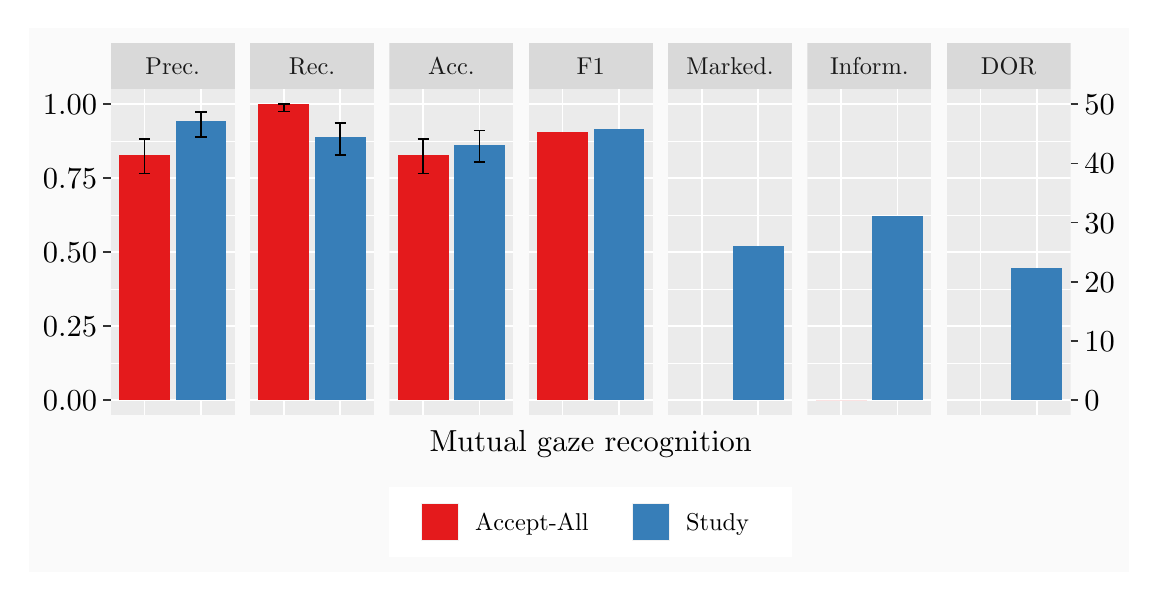
\begin{tikzpicture}[x=1pt,y=1pt]
\definecolor{fillColor}{RGB}{255,255,255}
\path[use as bounding box,fill=fillColor,fill opacity=0.00] (0,0) rectangle (398.34,196.94);
\begin{scope}
\path[clip] (  0.00,  0.00) rectangle (398.34,196.94);
\definecolor{drawColor}{RGB}{255,255,255}
\definecolor{fillColor}{gray}{0.98}

\path[draw=drawColor,line width= 0.6pt,line join=round,line cap=round,fill=fillColor] (  0.00,  0.00) rectangle (398.34,196.94);
\end{scope}
\begin{scope}
\path[clip] ( 30.00, 56.97) rectangle ( 74.84,174.63);
\definecolor{fillColor}{gray}{0.92}

\path[fill=fillColor] ( 30.00, 56.97) rectangle ( 74.84,174.63);
\definecolor{drawColor}{RGB}{255,255,255}

\path[draw=drawColor,line width= 0.3pt,line join=round] ( 30.00, 75.69) --
	( 74.84, 75.69);

\path[draw=drawColor,line width= 0.3pt,line join=round] ( 30.00,102.43) --
	( 74.84,102.43);

\path[draw=drawColor,line width= 0.3pt,line join=round] ( 30.00,129.17) --
	( 74.84,129.17);

\path[draw=drawColor,line width= 0.3pt,line join=round] ( 30.00,155.92) --
	( 74.84,155.92);

\path[draw=drawColor,line width= 0.6pt,line join=round] ( 30.00, 62.32) --
	( 74.84, 62.32);

\path[draw=drawColor,line width= 0.6pt,line join=round] ( 30.00, 89.06) --
	( 74.84, 89.06);

\path[draw=drawColor,line width= 0.6pt,line join=round] ( 30.00,115.80) --
	( 74.84,115.80);

\path[draw=drawColor,line width= 0.6pt,line join=round] ( 30.00,142.54) --
	( 74.84,142.54);

\path[draw=drawColor,line width= 0.6pt,line join=round] ( 30.00,169.29) --
	( 74.84,169.29);

\path[draw=drawColor,line width= 0.6pt,line join=round] ( 42.23, 56.97) --
	( 42.23,174.63);

\path[draw=drawColor,line width= 0.6pt,line join=round] ( 62.61, 56.97) --
	( 62.61,174.63);
\definecolor{fillColor}{RGB}{228,26,28}

\path[fill=fillColor] ( 33.06, 62.32) rectangle ( 51.40,151.05);
\definecolor{fillColor}{RGB}{55,126,184}

\path[fill=fillColor] ( 53.44, 62.32) rectangle ( 71.78,163.08);
\definecolor{drawColor}{RGB}{0,0,0}

\path[draw=drawColor,line width= 0.6pt,line join=round] ( 60.57,166.57) --
	( 64.65,166.57);

\path[draw=drawColor,line width= 0.6pt,line join=round] ( 62.61,166.57) --
	( 62.61,157.41);

\path[draw=drawColor,line width= 0.6pt,line join=round] ( 60.57,157.41) --
	( 64.65,157.41);

\path[draw=drawColor,line width= 0.6pt,line join=round] ( 40.19,156.66) --
	( 44.27,156.66);

\path[draw=drawColor,line width= 0.6pt,line join=round] ( 42.23,156.66) --
	( 42.23,144.22);

\path[draw=drawColor,line width= 0.6pt,line join=round] ( 40.19,144.22) --
	( 44.27,144.22);
\end{scope}
\begin{scope}
\path[clip] ( 80.34, 56.97) rectangle (125.18,174.63);
\definecolor{fillColor}{gray}{0.92}

\path[fill=fillColor] ( 80.34, 56.97) rectangle (125.18,174.63);
\definecolor{drawColor}{RGB}{255,255,255}

\path[draw=drawColor,line width= 0.3pt,line join=round] ( 80.34, 75.69) --
	(125.18, 75.69);

\path[draw=drawColor,line width= 0.3pt,line join=round] ( 80.34,102.43) --
	(125.18,102.43);

\path[draw=drawColor,line width= 0.3pt,line join=round] ( 80.34,129.17) --
	(125.18,129.17);

\path[draw=drawColor,line width= 0.3pt,line join=round] ( 80.34,155.92) --
	(125.18,155.92);

\path[draw=drawColor,line width= 0.6pt,line join=round] ( 80.34, 62.32) --
	(125.18, 62.32);

\path[draw=drawColor,line width= 0.6pt,line join=round] ( 80.34, 89.06) --
	(125.18, 89.06);

\path[draw=drawColor,line width= 0.6pt,line join=round] ( 80.34,115.80) --
	(125.18,115.80);

\path[draw=drawColor,line width= 0.6pt,line join=round] ( 80.34,142.54) --
	(125.18,142.54);

\path[draw=drawColor,line width= 0.6pt,line join=round] ( 80.34,169.29) --
	(125.18,169.29);

\path[draw=drawColor,line width= 0.6pt,line join=round] ( 92.57, 56.97) --
	( 92.57,174.63);

\path[draw=drawColor,line width= 0.6pt,line join=round] (112.95, 56.97) --
	(112.95,174.63);
\definecolor{fillColor}{RGB}{228,26,28}

\path[fill=fillColor] ( 83.40, 62.32) rectangle (101.74,169.29);
\definecolor{fillColor}{RGB}{55,126,184}

\path[fill=fillColor] (103.78, 62.32) rectangle (122.13,157.56);
\definecolor{drawColor}{RGB}{0,0,0}

\path[draw=drawColor,line width= 0.6pt,line join=round] (110.92,162.45) --
	(114.99,162.45);

\path[draw=drawColor,line width= 0.6pt,line join=round] (112.95,162.45) --
	(112.95,150.90);

\path[draw=drawColor,line width= 0.6pt,line join=round] (110.92,150.90) --
	(114.99,150.90);

\path[draw=drawColor,line width= 0.6pt,line join=round] ( 90.53,169.29) --
	( 94.61,169.29);

\path[draw=drawColor,line width= 0.6pt,line join=round] ( 92.57,169.29) --
	( 92.57,166.62);

\path[draw=drawColor,line width= 0.6pt,line join=round] ( 90.53,166.62) --
	( 94.61,166.62);
\end{scope}
\begin{scope}
\path[clip] (130.68, 56.97) rectangle (175.53,174.63);
\definecolor{fillColor}{gray}{0.92}

\path[fill=fillColor] (130.68, 56.97) rectangle (175.53,174.63);
\definecolor{drawColor}{RGB}{255,255,255}

\path[draw=drawColor,line width= 0.3pt,line join=round] (130.68, 75.69) --
	(175.53, 75.69);

\path[draw=drawColor,line width= 0.3pt,line join=round] (130.68,102.43) --
	(175.53,102.43);

\path[draw=drawColor,line width= 0.3pt,line join=round] (130.68,129.17) --
	(175.53,129.17);

\path[draw=drawColor,line width= 0.3pt,line join=round] (130.68,155.92) --
	(175.53,155.92);

\path[draw=drawColor,line width= 0.6pt,line join=round] (130.68, 62.32) --
	(175.53, 62.32);

\path[draw=drawColor,line width= 0.6pt,line join=round] (130.68, 89.06) --
	(175.53, 89.06);

\path[draw=drawColor,line width= 0.6pt,line join=round] (130.68,115.80) --
	(175.53,115.80);

\path[draw=drawColor,line width= 0.6pt,line join=round] (130.68,142.54) --
	(175.53,142.54);

\path[draw=drawColor,line width= 0.6pt,line join=round] (130.68,169.29) --
	(175.53,169.29);

\path[draw=drawColor,line width= 0.6pt,line join=round] (142.91, 56.97) --
	(142.91,174.63);

\path[draw=drawColor,line width= 0.6pt,line join=round] (163.30, 56.97) --
	(163.30,174.63);
\definecolor{fillColor}{RGB}{228,26,28}

\path[fill=fillColor] (133.74, 62.32) rectangle (152.09,151.05);
\definecolor{fillColor}{RGB}{55,126,184}

\path[fill=fillColor] (154.12, 62.32) rectangle (172.47,154.70);
\definecolor{drawColor}{RGB}{0,0,0}

\path[draw=drawColor,line width= 0.6pt,line join=round] (161.26,159.73) --
	(165.33,159.73);

\path[draw=drawColor,line width= 0.6pt,line join=round] (163.30,159.73) --
	(163.30,148.31);

\path[draw=drawColor,line width= 0.6pt,line join=round] (161.26,148.31) --
	(165.33,148.31);

\path[draw=drawColor,line width= 0.6pt,line join=round] (140.88,156.66) --
	(144.95,156.66);

\path[draw=drawColor,line width= 0.6pt,line join=round] (142.91,156.66) --
	(142.91,144.22);

\path[draw=drawColor,line width= 0.6pt,line join=round] (140.88,144.22) --
	(144.95,144.22);
\end{scope}
\begin{scope}
\path[clip] (181.03, 56.97) rectangle (225.87,174.63);
\definecolor{fillColor}{gray}{0.92}

\path[fill=fillColor] (181.03, 56.97) rectangle (225.87,174.63);
\definecolor{drawColor}{RGB}{255,255,255}

\path[draw=drawColor,line width= 0.3pt,line join=round] (181.03, 75.69) --
	(225.87, 75.69);

\path[draw=drawColor,line width= 0.3pt,line join=round] (181.03,102.43) --
	(225.87,102.43);

\path[draw=drawColor,line width= 0.3pt,line join=round] (181.03,129.17) --
	(225.87,129.17);

\path[draw=drawColor,line width= 0.3pt,line join=round] (181.03,155.92) --
	(225.87,155.92);

\path[draw=drawColor,line width= 0.6pt,line join=round] (181.03, 62.32) --
	(225.87, 62.32);

\path[draw=drawColor,line width= 0.6pt,line join=round] (181.03, 89.06) --
	(225.87, 89.06);

\path[draw=drawColor,line width= 0.6pt,line join=round] (181.03,115.80) --
	(225.87,115.80);

\path[draw=drawColor,line width= 0.6pt,line join=round] (181.03,142.54) --
	(225.87,142.54);

\path[draw=drawColor,line width= 0.6pt,line join=round] (181.03,169.29) --
	(225.87,169.29);

\path[draw=drawColor,line width= 0.6pt,line join=round] (193.25, 56.97) --
	(193.25,174.63);

\path[draw=drawColor,line width= 0.6pt,line join=round] (213.64, 56.97) --
	(213.64,174.63);
\definecolor{fillColor}{RGB}{228,26,28}

\path[fill=fillColor] (184.08, 62.32) rectangle (202.43,159.32);
\definecolor{fillColor}{RGB}{55,126,184}

\path[fill=fillColor] (204.47, 62.32) rectangle (222.81,160.25);
\end{scope}
\begin{scope}
\path[clip] (231.37, 56.97) rectangle (276.21,174.63);
\definecolor{fillColor}{gray}{0.92}

\path[fill=fillColor] (231.37, 56.97) rectangle (276.21,174.63);
\definecolor{drawColor}{RGB}{255,255,255}

\path[draw=drawColor,line width= 0.3pt,line join=round] (231.37, 75.69) --
	(276.21, 75.69);

\path[draw=drawColor,line width= 0.3pt,line join=round] (231.37,102.43) --
	(276.21,102.43);

\path[draw=drawColor,line width= 0.3pt,line join=round] (231.37,129.17) --
	(276.21,129.17);

\path[draw=drawColor,line width= 0.3pt,line join=round] (231.37,155.92) --
	(276.21,155.92);

\path[draw=drawColor,line width= 0.6pt,line join=round] (231.37, 62.32) --
	(276.21, 62.32);

\path[draw=drawColor,line width= 0.6pt,line join=round] (231.37, 89.06) --
	(276.21, 89.06);

\path[draw=drawColor,line width= 0.6pt,line join=round] (231.37,115.80) --
	(276.21,115.80);

\path[draw=drawColor,line width= 0.6pt,line join=round] (231.37,142.54) --
	(276.21,142.54);

\path[draw=drawColor,line width= 0.6pt,line join=round] (231.37,169.29) --
	(276.21,169.29);

\path[draw=drawColor,line width= 0.6pt,line join=round] (243.60, 56.97) --
	(243.60,174.63);

\path[draw=drawColor,line width= 0.6pt,line join=round] (263.98, 56.97) --
	(263.98,174.63);
\definecolor{fillColor}{RGB}{55,126,184}

\path[fill=fillColor] (254.81, 62.32) rectangle (273.15,118.05);
\end{scope}
\begin{scope}
\path[clip] (281.71, 56.97) rectangle (326.55,174.63);
\definecolor{fillColor}{gray}{0.92}

\path[fill=fillColor] (281.71, 56.97) rectangle (326.55,174.63);
\definecolor{drawColor}{RGB}{255,255,255}

\path[draw=drawColor,line width= 0.3pt,line join=round] (281.71, 75.69) --
	(326.55, 75.69);

\path[draw=drawColor,line width= 0.3pt,line join=round] (281.71,102.43) --
	(326.55,102.43);

\path[draw=drawColor,line width= 0.3pt,line join=round] (281.71,129.17) --
	(326.55,129.17);

\path[draw=drawColor,line width= 0.3pt,line join=round] (281.71,155.92) --
	(326.55,155.92);

\path[draw=drawColor,line width= 0.6pt,line join=round] (281.71, 62.32) --
	(326.55, 62.32);

\path[draw=drawColor,line width= 0.6pt,line join=round] (281.71, 89.06) --
	(326.55, 89.06);

\path[draw=drawColor,line width= 0.6pt,line join=round] (281.71,115.80) --
	(326.55,115.80);

\path[draw=drawColor,line width= 0.6pt,line join=round] (281.71,142.54) --
	(326.55,142.54);

\path[draw=drawColor,line width= 0.6pt,line join=round] (281.71,169.29) --
	(326.55,169.29);

\path[draw=drawColor,line width= 0.6pt,line join=round] (293.94, 56.97) --
	(293.94,174.63);

\path[draw=drawColor,line width= 0.6pt,line join=round] (314.32, 56.97) --
	(314.32,174.63);
\definecolor{fillColor}{RGB}{228,26,28}

\path[fill=fillColor] (284.77, 62.32) rectangle (303.11, 62.32);
\definecolor{fillColor}{RGB}{55,126,184}

\path[fill=fillColor] (305.15, 62.32) rectangle (323.49,129.04);
\end{scope}
\begin{scope}
\path[clip] (332.05, 56.97) rectangle (376.89,174.63);
\definecolor{fillColor}{gray}{0.92}

\path[fill=fillColor] (332.05, 56.97) rectangle (376.89,174.63);
\definecolor{drawColor}{RGB}{255,255,255}

\path[draw=drawColor,line width= 0.3pt,line join=round] (332.05, 75.69) --
	(376.89, 75.69);

\path[draw=drawColor,line width= 0.3pt,line join=round] (332.05,102.43) --
	(376.89,102.43);

\path[draw=drawColor,line width= 0.3pt,line join=round] (332.05,129.17) --
	(376.89,129.17);

\path[draw=drawColor,line width= 0.3pt,line join=round] (332.05,155.92) --
	(376.89,155.92);

\path[draw=drawColor,line width= 0.6pt,line join=round] (332.05, 62.32) --
	(376.89, 62.32);

\path[draw=drawColor,line width= 0.6pt,line join=round] (332.05, 89.06) --
	(376.89, 89.06);

\path[draw=drawColor,line width= 0.6pt,line join=round] (332.05,115.80) --
	(376.89,115.80);

\path[draw=drawColor,line width= 0.6pt,line join=round] (332.05,142.54) --
	(376.89,142.54);

\path[draw=drawColor,line width= 0.6pt,line join=round] (332.05,169.29) --
	(376.89,169.29);

\path[draw=drawColor,line width= 0.6pt,line join=round] (344.28, 56.97) --
	(344.28,174.63);

\path[draw=drawColor,line width= 0.6pt,line join=round] (364.66, 56.97) --
	(364.66,174.63);
\definecolor{fillColor}{RGB}{55,126,184}

\path[fill=fillColor] (355.49, 62.32) rectangle (373.83,110.12);
\end{scope}
\begin{scope}
\path[clip] ( 30.00,174.63) rectangle ( 74.84,191.44);
\definecolor{fillColor}{gray}{0.85}

\path[fill=fillColor] ( 30.00,174.63) rectangle ( 74.84,191.44);
\definecolor{drawColor}{gray}{0.10}

\node[text=drawColor,anchor=base,inner sep=0pt, outer sep=0pt, scale=  0.88] at ( 52.42,180.01) {Prec.};
\end{scope}
\begin{scope}
\path[clip] ( 80.34,174.63) rectangle (125.18,191.44);
\definecolor{fillColor}{gray}{0.85}

\path[fill=fillColor] ( 80.34,174.63) rectangle (125.18,191.44);
\definecolor{drawColor}{gray}{0.10}

\node[text=drawColor,anchor=base,inner sep=0pt, outer sep=0pt, scale=  0.88] at (102.76,180.01) {Rec.};
\end{scope}
\begin{scope}
\path[clip] (130.68,174.63) rectangle (175.53,191.44);
\definecolor{fillColor}{gray}{0.85}

\path[fill=fillColor] (130.68,174.63) rectangle (175.53,191.44);
\definecolor{drawColor}{gray}{0.10}

\node[text=drawColor,anchor=base,inner sep=0pt, outer sep=0pt, scale=  0.88] at (153.10,180.01) {Acc.};
\end{scope}
\begin{scope}
\path[clip] (181.03,174.63) rectangle (225.87,191.44);
\definecolor{fillColor}{gray}{0.85}

\path[fill=fillColor] (181.03,174.63) rectangle (225.87,191.44);
\definecolor{drawColor}{gray}{0.10}

\node[text=drawColor,anchor=base,inner sep=0pt, outer sep=0pt, scale=  0.88] at (203.45,180.01) {F1};
\end{scope}
\begin{scope}
\path[clip] (231.37,174.63) rectangle (276.21,191.44);
\definecolor{fillColor}{gray}{0.85}

\path[fill=fillColor] (231.37,174.63) rectangle (276.21,191.44);
\definecolor{drawColor}{gray}{0.10}

\node[text=drawColor,anchor=base,inner sep=0pt, outer sep=0pt, scale=  0.88] at (253.79,180.01) {Marked.};
\end{scope}
\begin{scope}
\path[clip] (281.71,174.63) rectangle (326.55,191.44);
\definecolor{fillColor}{gray}{0.85}

\path[fill=fillColor] (281.71,174.63) rectangle (326.55,191.44);
\definecolor{drawColor}{gray}{0.10}

\node[text=drawColor,anchor=base,inner sep=0pt, outer sep=0pt, scale=  0.88] at (304.13,180.01) {Inform.};
\end{scope}
\begin{scope}
\path[clip] (332.05,174.63) rectangle (376.89,191.44);
\definecolor{fillColor}{gray}{0.85}

\path[fill=fillColor] (332.05,174.63) rectangle (376.89,191.44);
\definecolor{drawColor}{gray}{0.10}

\node[text=drawColor,anchor=base,inner sep=0pt, outer sep=0pt, scale=  0.88] at (354.47,180.01) {DOR};
\end{scope}
\begin{scope}
\path[clip] (  0.00,  0.00) rectangle (398.34,196.94);
\definecolor{drawColor}{RGB}{0,0,0}

\node[text=drawColor,anchor=base east,inner sep=0pt, outer sep=0pt, scale=  1.10] at ( 25.05, 58.53) {0.00};

\node[text=drawColor,anchor=base east,inner sep=0pt, outer sep=0pt, scale=  1.10] at ( 25.05, 85.28) {0.25};

\node[text=drawColor,anchor=base east,inner sep=0pt, outer sep=0pt, scale=  1.10] at ( 25.05,112.02) {0.50};

\node[text=drawColor,anchor=base east,inner sep=0pt, outer sep=0pt, scale=  1.10] at ( 25.05,138.76) {0.75};

\node[text=drawColor,anchor=base east,inner sep=0pt, outer sep=0pt, scale=  1.10] at ( 25.05,165.50) {1.00};
\end{scope}
\begin{scope}
\path[clip] (  0.00,  0.00) rectangle (398.34,196.94);
\definecolor{drawColor}{gray}{0.20}

\path[draw=drawColor,line width= 0.6pt,line join=round] ( 27.25, 62.32) --
	( 30.00, 62.32);

\path[draw=drawColor,line width= 0.6pt,line join=round] ( 27.25, 89.06) --
	( 30.00, 89.06);

\path[draw=drawColor,line width= 0.6pt,line join=round] ( 27.25,115.80) --
	( 30.00,115.80);

\path[draw=drawColor,line width= 0.6pt,line join=round] ( 27.25,142.54) --
	( 30.00,142.54);

\path[draw=drawColor,line width= 0.6pt,line join=round] ( 27.25,169.29) --
	( 30.00,169.29);
\end{scope}
\begin{scope}
\path[clip] (  0.00,  0.00) rectangle (398.34,196.94);
\definecolor{drawColor}{gray}{0.20}

\path[draw=drawColor,line width= 0.6pt,line join=round] (376.89, 62.32) --
	(379.64, 62.32);

\path[draw=drawColor,line width= 0.6pt,line join=round] (376.89, 83.71) --
	(379.64, 83.71);

\path[draw=drawColor,line width= 0.6pt,line join=round] (376.89,105.11) --
	(379.64,105.11);

\path[draw=drawColor,line width= 0.6pt,line join=round] (376.89,126.50) --
	(379.64,126.50);

\path[draw=drawColor,line width= 0.6pt,line join=round] (376.89,147.89) --
	(379.64,147.89);

\path[draw=drawColor,line width= 0.6pt,line join=round] (376.89,169.29) --
	(379.64,169.29);
\end{scope}
\begin{scope}
\path[clip] (  0.00,  0.00) rectangle (398.34,196.94);
\definecolor{drawColor}{RGB}{0,0,0}

\node[text=drawColor,anchor=base west,inner sep=0pt, outer sep=0pt, scale=  1.10] at (381.84, 58.53) {0};

\node[text=drawColor,anchor=base west,inner sep=0pt, outer sep=0pt, scale=  1.10] at (381.84, 79.93) {10};

\node[text=drawColor,anchor=base west,inner sep=0pt, outer sep=0pt, scale=  1.10] at (381.84,101.32) {20};

\node[text=drawColor,anchor=base west,inner sep=0pt, outer sep=0pt, scale=  1.10] at (381.84,122.71) {30};

\node[text=drawColor,anchor=base west,inner sep=0pt, outer sep=0pt, scale=  1.10] at (381.84,144.10) {40};

\node[text=drawColor,anchor=base west,inner sep=0pt, outer sep=0pt, scale=  1.10] at (381.84,165.50) {50};
\end{scope}
\begin{scope}
\path[clip] (  0.00,  0.00) rectangle (398.34,196.94);
\definecolor{drawColor}{RGB}{0,0,0}

\node[text=drawColor,anchor=base,inner sep=0pt, outer sep=0pt, scale=  1.10] at (203.45, 43.90) {Mutual gaze recognition};
\end{scope}
\begin{scope}
\path[clip] (  0.00,  0.00) rectangle (398.34,196.94);
\definecolor{fillColor}{RGB}{255,255,255}

\path[fill=fillColor] (130.72,  5.50) rectangle (276.17, 30.95);
\end{scope}
\begin{scope}
\path[clip] (  0.00,  0.00) rectangle (398.34,196.94);
\definecolor{drawColor}{RGB}{255,255,255}
\definecolor{fillColor}{gray}{0.95}

\path[draw=drawColor,line width= 0.6pt,line join=round,line cap=round,fill=fillColor] (141.72, 11.00) rectangle (156.18, 25.45);
\end{scope}
\begin{scope}
\path[clip] (  0.00,  0.00) rectangle (398.34,196.94);
\definecolor{fillColor}{RGB}{228,26,28}

\path[fill=fillColor] (142.43, 11.71) rectangle (155.46, 24.74);
\end{scope}
\begin{scope}
\path[clip] (  0.00,  0.00) rectangle (398.34,196.94);
\definecolor{drawColor}{RGB}{255,255,255}
\definecolor{fillColor}{gray}{0.95}

\path[draw=drawColor,line width= 0.6pt,line join=round,line cap=round,fill=fillColor] (217.99, 11.00) rectangle (232.44, 25.45);
\end{scope}
\begin{scope}
\path[clip] (  0.00,  0.00) rectangle (398.34,196.94);
\definecolor{fillColor}{RGB}{55,126,184}

\path[fill=fillColor] (218.70, 11.71) rectangle (231.73, 24.74);
\end{scope}
\begin{scope}
\path[clip] (  0.00,  0.00) rectangle (398.34,196.94);
\definecolor{drawColor}{RGB}{0,0,0}

\node[text=drawColor,anchor=base west,inner sep=0pt, outer sep=0pt, scale=  0.88] at (161.68, 15.20) {Accept-All};
\end{scope}
\begin{scope}
\path[clip] (  0.00,  0.00) rectangle (398.34,196.94);
\definecolor{drawColor}{RGB}{0,0,0}

\node[text=drawColor,anchor=base west,inner sep=0pt, outer sep=0pt, scale=  0.88] at (237.94, 15.20) {Study};
\end{scope}
\end{tikzpicture}

      }
      \vspace{-70pt}
    \end{figure}
    \begin{figure}[htb]
      \resizebox{\textwidth}{!}{%
        % Created by tikzDevice version 0.12
% !TEX encoding = UTF-8 Unicode
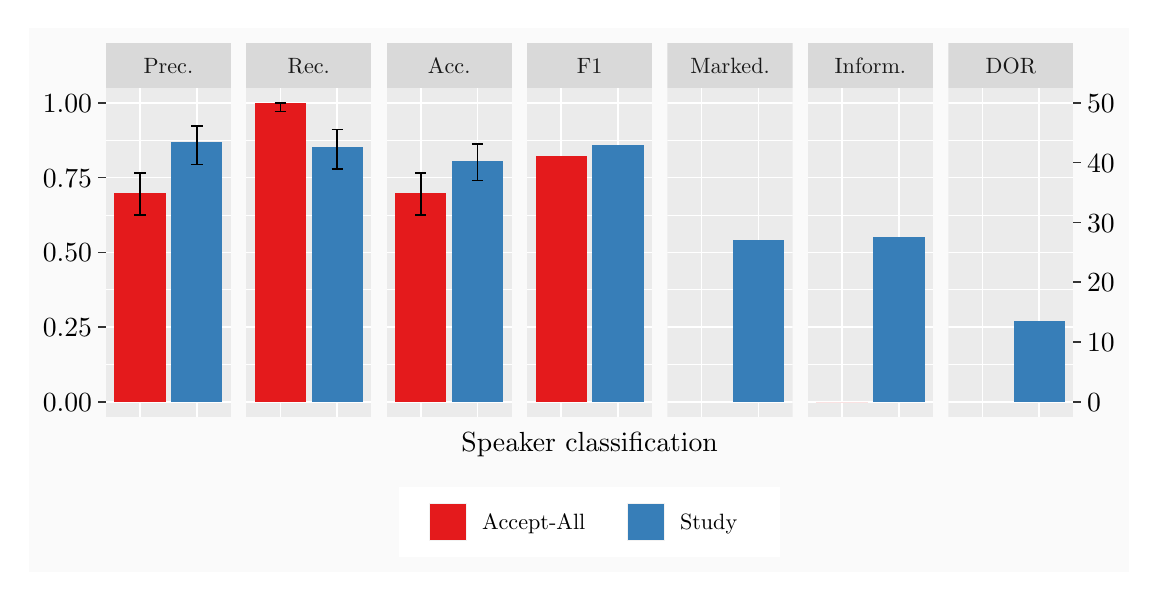
\begin{tikzpicture}[x=1pt,y=1pt]
\definecolor{fillColor}{RGB}{255,255,255}
\path[use as bounding box,fill=fillColor,fill opacity=0.00] (0,0) rectangle (398.34,196.94);
\begin{scope}
\path[clip] (  0.00,  0.00) rectangle (398.34,196.94);
\definecolor{drawColor}{RGB}{255,255,255}
\definecolor{fillColor}{gray}{0.98}

\path[draw=drawColor,line width= 0.6pt,line join=round,line cap=round,fill=fillColor] (  0.00,  0.00) rectangle (398.34,196.94);
\end{scope}
\begin{scope}
\path[clip] ( 28.22, 56.29) rectangle ( 73.46,175.18);
\definecolor{fillColor}{gray}{0.92}

\path[fill=fillColor] ( 28.22, 56.29) rectangle ( 73.46,175.18);
\definecolor{drawColor}{RGB}{255,255,255}

\path[draw=drawColor,line width= 0.3pt,line join=round] ( 28.22, 75.20) --
	( 73.46, 75.20);

\path[draw=drawColor,line width= 0.3pt,line join=round] ( 28.22,102.22) --
	( 73.46,102.22);

\path[draw=drawColor,line width= 0.3pt,line join=round] ( 28.22,129.25) --
	( 73.46,129.25);

\path[draw=drawColor,line width= 0.3pt,line join=round] ( 28.22,156.27) --
	( 73.46,156.27);

\path[draw=drawColor,line width= 0.6pt,line join=round] ( 28.22, 61.69) --
	( 73.46, 61.69);

\path[draw=drawColor,line width= 0.6pt,line join=round] ( 28.22, 88.71) --
	( 73.46, 88.71);

\path[draw=drawColor,line width= 0.6pt,line join=round] ( 28.22,115.74) --
	( 73.46,115.74);

\path[draw=drawColor,line width= 0.6pt,line join=round] ( 28.22,142.76) --
	( 73.46,142.76);

\path[draw=drawColor,line width= 0.6pt,line join=round] ( 28.22,169.78) --
	( 73.46,169.78);

\path[draw=drawColor,line width= 0.6pt,line join=round] ( 40.56, 56.29) --
	( 40.56,175.18);

\path[draw=drawColor,line width= 0.6pt,line join=round] ( 61.12, 56.29) --
	( 61.12,175.18);
\definecolor{fillColor}{RGB}{228,26,28}

\path[fill=fillColor] ( 31.31, 61.69) rectangle ( 49.81,137.23);
\definecolor{fillColor}{RGB}{55,126,184}

\path[fill=fillColor] ( 51.87, 61.69) rectangle ( 70.38,155.49);
\definecolor{drawColor}{RGB}{0,0,0}

\path[draw=drawColor,line width= 0.6pt,line join=round] ( 59.07,161.40) --
	( 63.18,161.40);

\path[draw=drawColor,line width= 0.6pt,line join=round] ( 61.12,161.40) --
	( 61.12,147.53);

\path[draw=drawColor,line width= 0.6pt,line join=round] ( 59.07,147.53) --
	( 63.18,147.53);

\path[draw=drawColor,line width= 0.6pt,line join=round] ( 38.50,144.44) --
	( 42.62,144.44);

\path[draw=drawColor,line width= 0.6pt,line join=round] ( 40.56,144.44) --
	( 40.56,129.28);

\path[draw=drawColor,line width= 0.6pt,line join=round] ( 38.50,129.28) --
	( 42.62,129.28);
\end{scope}
\begin{scope}
\path[clip] ( 78.96, 56.29) rectangle (124.20,175.18);
\definecolor{fillColor}{gray}{0.92}

\path[fill=fillColor] ( 78.96, 56.29) rectangle (124.20,175.18);
\definecolor{drawColor}{RGB}{255,255,255}

\path[draw=drawColor,line width= 0.3pt,line join=round] ( 78.96, 75.20) --
	(124.20, 75.20);

\path[draw=drawColor,line width= 0.3pt,line join=round] ( 78.96,102.22) --
	(124.20,102.22);

\path[draw=drawColor,line width= 0.3pt,line join=round] ( 78.96,129.25) --
	(124.20,129.25);

\path[draw=drawColor,line width= 0.3pt,line join=round] ( 78.96,156.27) --
	(124.20,156.27);

\path[draw=drawColor,line width= 0.6pt,line join=round] ( 78.96, 61.69) --
	(124.20, 61.69);

\path[draw=drawColor,line width= 0.6pt,line join=round] ( 78.96, 88.71) --
	(124.20, 88.71);

\path[draw=drawColor,line width= 0.6pt,line join=round] ( 78.96,115.74) --
	(124.20,115.74);

\path[draw=drawColor,line width= 0.6pt,line join=round] ( 78.96,142.76) --
	(124.20,142.76);

\path[draw=drawColor,line width= 0.6pt,line join=round] ( 78.96,169.78) --
	(124.20,169.78);

\path[draw=drawColor,line width= 0.6pt,line join=round] ( 91.30, 56.29) --
	( 91.30,175.18);

\path[draw=drawColor,line width= 0.6pt,line join=round] (111.86, 56.29) --
	(111.86,175.18);
\definecolor{fillColor}{RGB}{228,26,28}

\path[fill=fillColor] ( 82.05, 61.69) rectangle (100.55,169.78);
\definecolor{fillColor}{RGB}{55,126,184}

\path[fill=fillColor] (102.61, 61.69) rectangle (121.12,153.96);
\definecolor{drawColor}{RGB}{0,0,0}

\path[draw=drawColor,line width= 0.6pt,line join=round] (109.81,160.15) --
	(113.92,160.15);

\path[draw=drawColor,line width= 0.6pt,line join=round] (111.86,160.15) --
	(111.86,145.85);

\path[draw=drawColor,line width= 0.6pt,line join=round] (109.81,145.85) --
	(113.92,145.85);

\path[draw=drawColor,line width= 0.6pt,line join=round] ( 89.24,169.78) --
	( 93.36,169.78);

\path[draw=drawColor,line width= 0.6pt,line join=round] ( 91.30,169.78) --
	( 91.30,166.59);

\path[draw=drawColor,line width= 0.6pt,line join=round] ( 89.24,166.59) --
	( 93.36,166.59);
\end{scope}
\begin{scope}
\path[clip] (129.70, 56.29) rectangle (174.94,175.18);
\definecolor{fillColor}{gray}{0.92}

\path[fill=fillColor] (129.70, 56.29) rectangle (174.94,175.18);
\definecolor{drawColor}{RGB}{255,255,255}

\path[draw=drawColor,line width= 0.3pt,line join=round] (129.70, 75.20) --
	(174.94, 75.20);

\path[draw=drawColor,line width= 0.3pt,line join=round] (129.70,102.22) --
	(174.94,102.22);

\path[draw=drawColor,line width= 0.3pt,line join=round] (129.70,129.25) --
	(174.94,129.25);

\path[draw=drawColor,line width= 0.3pt,line join=round] (129.70,156.27) --
	(174.94,156.27);

\path[draw=drawColor,line width= 0.6pt,line join=round] (129.70, 61.69) --
	(174.94, 61.69);

\path[draw=drawColor,line width= 0.6pt,line join=round] (129.70, 88.71) --
	(174.94, 88.71);

\path[draw=drawColor,line width= 0.6pt,line join=round] (129.70,115.74) --
	(174.94,115.74);

\path[draw=drawColor,line width= 0.6pt,line join=round] (129.70,142.76) --
	(174.94,142.76);

\path[draw=drawColor,line width= 0.6pt,line join=round] (129.70,169.78) --
	(174.94,169.78);

\path[draw=drawColor,line width= 0.6pt,line join=round] (142.04, 56.29) --
	(142.04,175.18);

\path[draw=drawColor,line width= 0.6pt,line join=round] (162.60, 56.29) --
	(162.60,175.18);
\definecolor{fillColor}{RGB}{228,26,28}

\path[fill=fillColor] (132.78, 61.69) rectangle (151.29,137.23);
\definecolor{fillColor}{RGB}{55,126,184}

\path[fill=fillColor] (153.35, 61.69) rectangle (171.85,148.90);
\definecolor{drawColor}{RGB}{0,0,0}

\path[draw=drawColor,line width= 0.6pt,line join=round] (160.54,154.90) --
	(164.66,154.90);

\path[draw=drawColor,line width= 0.6pt,line join=round] (162.60,154.90) --
	(162.60,141.75);

\path[draw=drawColor,line width= 0.6pt,line join=round] (160.54,141.75) --
	(164.66,141.75);

\path[draw=drawColor,line width= 0.6pt,line join=round] (139.98,144.44) --
	(144.09,144.44);

\path[draw=drawColor,line width= 0.6pt,line join=round] (142.04,144.44) --
	(142.04,129.28);

\path[draw=drawColor,line width= 0.6pt,line join=round] (139.98,129.28) --
	(144.09,129.28);
\end{scope}
\begin{scope}
\path[clip] (180.44, 56.29) rectangle (225.68,175.18);
\definecolor{fillColor}{gray}{0.92}

\path[fill=fillColor] (180.44, 56.29) rectangle (225.68,175.18);
\definecolor{drawColor}{RGB}{255,255,255}

\path[draw=drawColor,line width= 0.3pt,line join=round] (180.44, 75.20) --
	(225.68, 75.20);

\path[draw=drawColor,line width= 0.3pt,line join=round] (180.44,102.22) --
	(225.68,102.22);

\path[draw=drawColor,line width= 0.3pt,line join=round] (180.44,129.25) --
	(225.68,129.25);

\path[draw=drawColor,line width= 0.3pt,line join=round] (180.44,156.27) --
	(225.68,156.27);

\path[draw=drawColor,line width= 0.6pt,line join=round] (180.44, 61.69) --
	(225.68, 61.69);

\path[draw=drawColor,line width= 0.6pt,line join=round] (180.44, 88.71) --
	(225.68, 88.71);

\path[draw=drawColor,line width= 0.6pt,line join=round] (180.44,115.74) --
	(225.68,115.74);

\path[draw=drawColor,line width= 0.6pt,line join=round] (180.44,142.76) --
	(225.68,142.76);

\path[draw=drawColor,line width= 0.6pt,line join=round] (180.44,169.78) --
	(225.68,169.78);

\path[draw=drawColor,line width= 0.6pt,line join=round] (192.78, 56.29) --
	(192.78,175.18);

\path[draw=drawColor,line width= 0.6pt,line join=round] (213.34, 56.29) --
	(213.34,175.18);
\definecolor{fillColor}{RGB}{228,26,28}

\path[fill=fillColor] (183.52, 61.69) rectangle (202.03,150.62);
\definecolor{fillColor}{RGB}{55,126,184}

\path[fill=fillColor] (204.09, 61.69) rectangle (222.59,154.72);
\end{scope}
\begin{scope}
\path[clip] (231.18, 56.29) rectangle (276.41,175.18);
\definecolor{fillColor}{gray}{0.92}

\path[fill=fillColor] (231.18, 56.29) rectangle (276.41,175.18);
\definecolor{drawColor}{RGB}{255,255,255}

\path[draw=drawColor,line width= 0.3pt,line join=round] (231.18, 75.20) --
	(276.41, 75.20);

\path[draw=drawColor,line width= 0.3pt,line join=round] (231.18,102.22) --
	(276.41,102.22);

\path[draw=drawColor,line width= 0.3pt,line join=round] (231.18,129.25) --
	(276.41,129.25);

\path[draw=drawColor,line width= 0.3pt,line join=round] (231.18,156.27) --
	(276.41,156.27);

\path[draw=drawColor,line width= 0.6pt,line join=round] (231.18, 61.69) --
	(276.41, 61.69);

\path[draw=drawColor,line width= 0.6pt,line join=round] (231.18, 88.71) --
	(276.41, 88.71);

\path[draw=drawColor,line width= 0.6pt,line join=round] (231.18,115.74) --
	(276.41,115.74);

\path[draw=drawColor,line width= 0.6pt,line join=round] (231.18,142.76) --
	(276.41,142.76);

\path[draw=drawColor,line width= 0.6pt,line join=round] (231.18,169.78) --
	(276.41,169.78);

\path[draw=drawColor,line width= 0.6pt,line join=round] (243.51, 56.29) --
	(243.51,175.18);

\path[draw=drawColor,line width= 0.6pt,line join=round] (264.08, 56.29) --
	(264.08,175.18);
\definecolor{fillColor}{RGB}{55,126,184}

\path[fill=fillColor] (254.82, 61.69) rectangle (273.33,120.11);
\end{scope}
\begin{scope}
\path[clip] (281.91, 56.29) rectangle (327.15,175.18);
\definecolor{fillColor}{gray}{0.92}

\path[fill=fillColor] (281.91, 56.29) rectangle (327.15,175.18);
\definecolor{drawColor}{RGB}{255,255,255}

\path[draw=drawColor,line width= 0.3pt,line join=round] (281.91, 75.20) --
	(327.15, 75.20);

\path[draw=drawColor,line width= 0.3pt,line join=round] (281.91,102.22) --
	(327.15,102.22);

\path[draw=drawColor,line width= 0.3pt,line join=round] (281.91,129.25) --
	(327.15,129.25);

\path[draw=drawColor,line width= 0.3pt,line join=round] (281.91,156.27) --
	(327.15,156.27);

\path[draw=drawColor,line width= 0.6pt,line join=round] (281.91, 61.69) --
	(327.15, 61.69);

\path[draw=drawColor,line width= 0.6pt,line join=round] (281.91, 88.71) --
	(327.15, 88.71);

\path[draw=drawColor,line width= 0.6pt,line join=round] (281.91,115.74) --
	(327.15,115.74);

\path[draw=drawColor,line width= 0.6pt,line join=round] (281.91,142.76) --
	(327.15,142.76);

\path[draw=drawColor,line width= 0.6pt,line join=round] (281.91,169.78) --
	(327.15,169.78);

\path[draw=drawColor,line width= 0.6pt,line join=round] (294.25, 56.29) --
	(294.25,175.18);

\path[draw=drawColor,line width= 0.6pt,line join=round] (314.82, 56.29) --
	(314.82,175.18);
\definecolor{fillColor}{RGB}{228,26,28}

\path[fill=fillColor] (285.00, 61.69) rectangle (303.51, 61.69);
\definecolor{fillColor}{RGB}{55,126,184}

\path[fill=fillColor] (305.56, 61.69) rectangle (324.07,121.33);
\end{scope}
\begin{scope}
\path[clip] (332.65, 56.29) rectangle (377.89,175.18);
\definecolor{fillColor}{gray}{0.92}

\path[fill=fillColor] (332.65, 56.29) rectangle (377.89,175.18);
\definecolor{drawColor}{RGB}{255,255,255}

\path[draw=drawColor,line width= 0.3pt,line join=round] (332.65, 75.20) --
	(377.89, 75.20);

\path[draw=drawColor,line width= 0.3pt,line join=round] (332.65,102.22) --
	(377.89,102.22);

\path[draw=drawColor,line width= 0.3pt,line join=round] (332.65,129.25) --
	(377.89,129.25);

\path[draw=drawColor,line width= 0.3pt,line join=round] (332.65,156.27) --
	(377.89,156.27);

\path[draw=drawColor,line width= 0.6pt,line join=round] (332.65, 61.69) --
	(377.89, 61.69);

\path[draw=drawColor,line width= 0.6pt,line join=round] (332.65, 88.71) --
	(377.89, 88.71);

\path[draw=drawColor,line width= 0.6pt,line join=round] (332.65,115.74) --
	(377.89,115.74);

\path[draw=drawColor,line width= 0.6pt,line join=round] (332.65,142.76) --
	(377.89,142.76);

\path[draw=drawColor,line width= 0.6pt,line join=round] (332.65,169.78) --
	(377.89,169.78);

\path[draw=drawColor,line width= 0.6pt,line join=round] (344.99, 56.29) --
	(344.99,175.18);

\path[draw=drawColor,line width= 0.6pt,line join=round] (365.55, 56.29) --
	(365.55,175.18);
\definecolor{fillColor}{RGB}{55,126,184}

\path[fill=fillColor] (356.30, 61.69) rectangle (374.81, 90.85);
\end{scope}
\begin{scope}
\path[clip] ( 28.22,175.18) rectangle ( 73.46,191.44);
\definecolor{fillColor}{gray}{0.85}

\path[fill=fillColor] ( 28.22,175.18) rectangle ( 73.46,191.44);
\definecolor{drawColor}{gray}{0.10}

\node[text=drawColor,anchor=base,inner sep=0pt, outer sep=0pt, scale=  0.80] at ( 50.84,180.56) {Prec.};
\end{scope}
\begin{scope}
\path[clip] ( 78.96,175.18) rectangle (124.20,191.44);
\definecolor{fillColor}{gray}{0.85}

\path[fill=fillColor] ( 78.96,175.18) rectangle (124.20,191.44);
\definecolor{drawColor}{gray}{0.10}

\node[text=drawColor,anchor=base,inner sep=0pt, outer sep=0pt, scale=  0.80] at (101.58,180.56) {Rec.};
\end{scope}
\begin{scope}
\path[clip] (129.70,175.18) rectangle (174.94,191.44);
\definecolor{fillColor}{gray}{0.85}

\path[fill=fillColor] (129.70,175.18) rectangle (174.94,191.44);
\definecolor{drawColor}{gray}{0.10}

\node[text=drawColor,anchor=base,inner sep=0pt, outer sep=0pt, scale=  0.80] at (152.32,180.56) {Acc.};
\end{scope}
\begin{scope}
\path[clip] (180.44,175.18) rectangle (225.68,191.44);
\definecolor{fillColor}{gray}{0.85}

\path[fill=fillColor] (180.44,175.18) rectangle (225.68,191.44);
\definecolor{drawColor}{gray}{0.10}

\node[text=drawColor,anchor=base,inner sep=0pt, outer sep=0pt, scale=  0.80] at (203.06,180.56) {F1};
\end{scope}
\begin{scope}
\path[clip] (231.18,175.18) rectangle (276.41,191.44);
\definecolor{fillColor}{gray}{0.85}

\path[fill=fillColor] (231.18,175.18) rectangle (276.41,191.44);
\definecolor{drawColor}{gray}{0.10}

\node[text=drawColor,anchor=base,inner sep=0pt, outer sep=0pt, scale=  0.80] at (253.80,180.56) {Marked.};
\end{scope}
\begin{scope}
\path[clip] (281.91,175.18) rectangle (327.15,191.44);
\definecolor{fillColor}{gray}{0.85}

\path[fill=fillColor] (281.91,175.18) rectangle (327.15,191.44);
\definecolor{drawColor}{gray}{0.10}

\node[text=drawColor,anchor=base,inner sep=0pt, outer sep=0pt, scale=  0.80] at (304.53,180.56) {Inform.};
\end{scope}
\begin{scope}
\path[clip] (332.65,175.18) rectangle (377.89,191.44);
\definecolor{fillColor}{gray}{0.85}

\path[fill=fillColor] (332.65,175.18) rectangle (377.89,191.44);
\definecolor{drawColor}{gray}{0.10}

\node[text=drawColor,anchor=base,inner sep=0pt, outer sep=0pt, scale=  0.80] at (355.27,180.56) {DOR};
\end{scope}
\begin{scope}
\path[clip] (  0.00,  0.00) rectangle (398.34,196.94);
\definecolor{drawColor}{RGB}{0,0,0}

\node[text=drawColor,anchor=base east,inner sep=0pt, outer sep=0pt, scale=  1.00] at ( 23.27, 58.25) {0.00};

\node[text=drawColor,anchor=base east,inner sep=0pt, outer sep=0pt, scale=  1.00] at ( 23.27, 85.27) {0.25};

\node[text=drawColor,anchor=base east,inner sep=0pt, outer sep=0pt, scale=  1.00] at ( 23.27,112.29) {0.50};

\node[text=drawColor,anchor=base east,inner sep=0pt, outer sep=0pt, scale=  1.00] at ( 23.27,139.31) {0.75};

\node[text=drawColor,anchor=base east,inner sep=0pt, outer sep=0pt, scale=  1.00] at ( 23.27,166.34) {1.00};
\end{scope}
\begin{scope}
\path[clip] (  0.00,  0.00) rectangle (398.34,196.94);
\definecolor{drawColor}{gray}{0.20}

\path[draw=drawColor,line width= 0.6pt,line join=round] ( 25.47, 61.69) --
	( 28.22, 61.69);

\path[draw=drawColor,line width= 0.6pt,line join=round] ( 25.47, 88.71) --
	( 28.22, 88.71);

\path[draw=drawColor,line width= 0.6pt,line join=round] ( 25.47,115.74) --
	( 28.22,115.74);

\path[draw=drawColor,line width= 0.6pt,line join=round] ( 25.47,142.76) --
	( 28.22,142.76);

\path[draw=drawColor,line width= 0.6pt,line join=round] ( 25.47,169.78) --
	( 28.22,169.78);
\end{scope}
\begin{scope}
\path[clip] (  0.00,  0.00) rectangle (398.34,196.94);
\definecolor{drawColor}{gray}{0.20}

\path[draw=drawColor,line width= 0.6pt,line join=round] (377.89, 61.69) --
	(380.64, 61.69);

\path[draw=drawColor,line width= 0.6pt,line join=round] (377.89, 83.31) --
	(380.64, 83.31);

\path[draw=drawColor,line width= 0.6pt,line join=round] (377.89,104.93) --
	(380.64,104.93);

\path[draw=drawColor,line width= 0.6pt,line join=round] (377.89,126.54) --
	(380.64,126.54);

\path[draw=drawColor,line width= 0.6pt,line join=round] (377.89,148.16) --
	(380.64,148.16);

\path[draw=drawColor,line width= 0.6pt,line join=round] (377.89,169.78) --
	(380.64,169.78);
\end{scope}
\begin{scope}
\path[clip] (  0.00,  0.00) rectangle (398.34,196.94);
\definecolor{drawColor}{RGB}{0,0,0}

\node[text=drawColor,anchor=base west,inner sep=0pt, outer sep=0pt, scale=  1.00] at (382.84, 58.25) {0};

\node[text=drawColor,anchor=base west,inner sep=0pt, outer sep=0pt, scale=  1.00] at (382.84, 79.86) {10};

\node[text=drawColor,anchor=base west,inner sep=0pt, outer sep=0pt, scale=  1.00] at (382.84,101.48) {20};

\node[text=drawColor,anchor=base west,inner sep=0pt, outer sep=0pt, scale=  1.00] at (382.84,123.10) {30};

\node[text=drawColor,anchor=base west,inner sep=0pt, outer sep=0pt, scale=  1.00] at (382.84,144.72) {40};

\node[text=drawColor,anchor=base west,inner sep=0pt, outer sep=0pt, scale=  1.00] at (382.84,166.34) {50};
\end{scope}
\begin{scope}
\path[clip] (  0.00,  0.00) rectangle (398.34,196.94);
\definecolor{drawColor}{RGB}{0,0,0}

\node[text=drawColor,anchor=base,inner sep=0pt, outer sep=0pt, scale=  1.00] at (203.06, 43.90) {Speaker classification};
\end{scope}
\begin{scope}
\path[clip] (  0.00,  0.00) rectangle (398.34,196.94);
\definecolor{fillColor}{RGB}{255,255,255}

\path[fill=fillColor] (134.22,  5.50) rectangle (271.89, 30.95);
\end{scope}
\begin{scope}
\path[clip] (  0.00,  0.00) rectangle (398.34,196.94);
\definecolor{drawColor}{RGB}{255,255,255}
\definecolor{fillColor}{gray}{0.95}

\path[draw=drawColor,line width= 0.6pt,line join=round,line cap=round,fill=fillColor] (144.72, 11.00) rectangle (159.18, 25.45);
\end{scope}
\begin{scope}
\path[clip] (  0.00,  0.00) rectangle (398.34,196.94);
\definecolor{fillColor}{RGB}{228,26,28}

\path[fill=fillColor] (145.43, 11.71) rectangle (158.46, 24.74);
\end{scope}
\begin{scope}
\path[clip] (  0.00,  0.00) rectangle (398.34,196.94);
\definecolor{drawColor}{RGB}{255,255,255}
\definecolor{fillColor}{gray}{0.95}

\path[draw=drawColor,line width= 0.6pt,line join=round,line cap=round,fill=fillColor] (216.28, 11.00) rectangle (230.73, 25.45);
\end{scope}
\begin{scope}
\path[clip] (  0.00,  0.00) rectangle (398.34,196.94);
\definecolor{fillColor}{RGB}{55,126,184}

\path[fill=fillColor] (216.99, 11.71) rectangle (230.02, 24.74);
\end{scope}
\begin{scope}
\path[clip] (  0.00,  0.00) rectangle (398.34,196.94);
\definecolor{drawColor}{RGB}{0,0,0}

\node[text=drawColor,anchor=base west,inner sep=0pt, outer sep=0pt, scale=  0.80] at (164.18, 15.47) {Accept-All};
\end{scope}
\begin{scope}
\path[clip] (  0.00,  0.00) rectangle (398.34,196.94);
\definecolor{drawColor}{RGB}{0,0,0}

\node[text=drawColor,anchor=base west,inner sep=0pt, outer sep=0pt, scale=  0.80] at (235.73, 15.47) {Study};
\end{scope}
\end{tikzpicture}

      }
    \end{figure}
    \end{column}%
      \begin{column}{.5\textwidth}
        \begin{center}
        \begin{scriptsize}
          Mutual Gaze Recognition
          \\ \vspace{10pt}
          \begin{tabular}{l | c | c }
                  & Baseline & Study \\ \hline
            \(P\) &  0.766 - 0.882&   \textbf{0.889 - 0.975} \\ 
            \(R\) &  \textbf{0.975 - 1.000} &  0.828 - 0.936 \\
           \end{tabular}
          \\ \vspace{10pt}
          \(M(G_S) = 0.52 \)\quad\(I(G_S) = 0.62\)\quad\( DOR(G_S) = 22\)
          \\ \vspace{10pt}
          Speaker classification
          \\ \vspace{10pt}
          \begin{tabular}{l | c | c }
                  & Baseline & Study \\ \hline
            \(P\) &  0.625 - 0.766 &   \textbf{0.794 - 0.922} \\ 
            \(R\) &  \textbf{0.970 - 1.00} &  0.779 - 0.911 \\
           \end{tabular}
          \\ \vspace{10pt}
          \(M(S_S) = 0.54 \)\quad\(I(S_S) = 0.55\)\quad\( DOR(S_S) = 13\)
          \end{scriptsize}
        \end{center}
   \end{column}%
   \end{columns}
  \end{frame}
  \begin{frame}{Addressee from mutual gaze \tiny{with 5\% confidence intervals}}
    \begin{columns}[T] % align columns
      \begin{column}{.5\textwidth}
        \begin{figure}[htb]
          \resizebox{\textwidth}{!}{%
            % Created by tikzDevice version 0.12
% !TEX encoding = UTF-8 Unicode
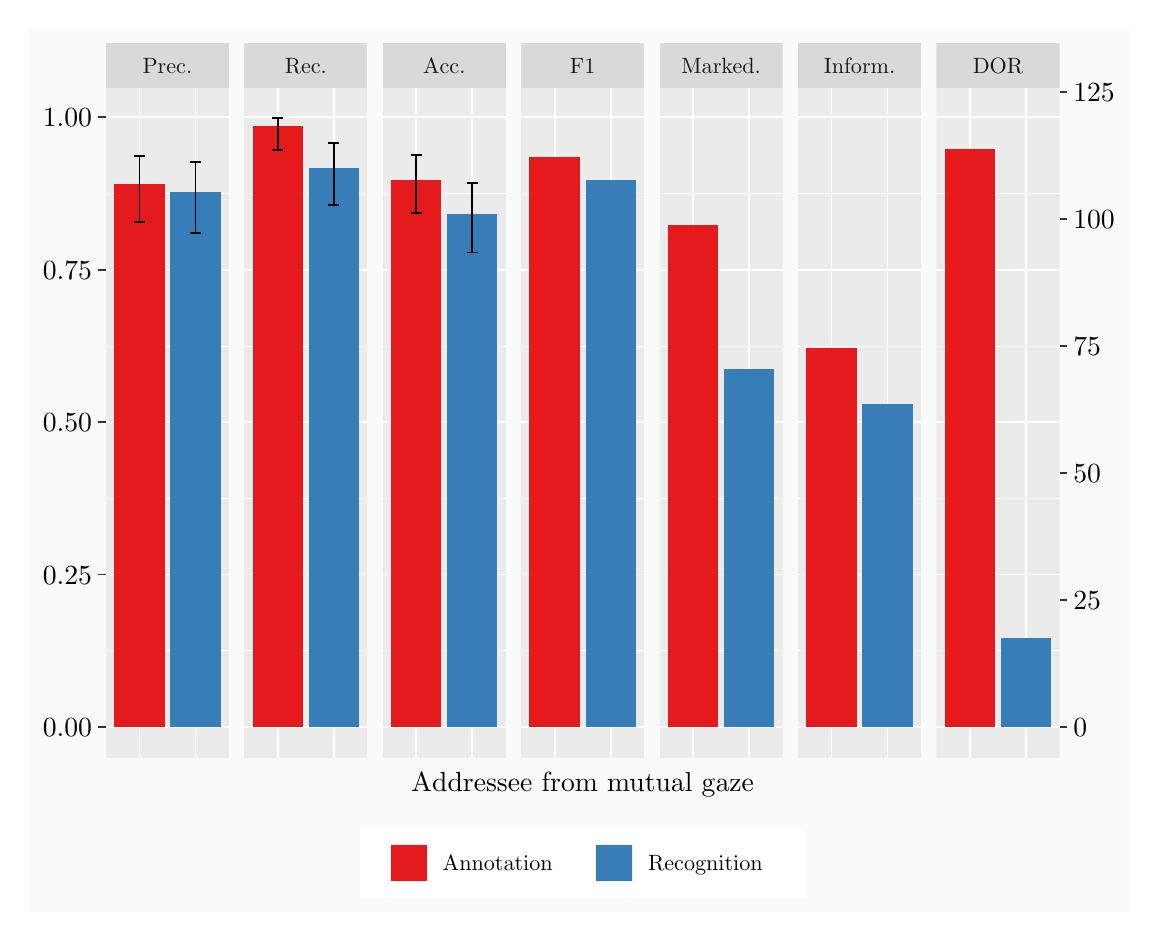
\begin{tikzpicture}[x=1pt,y=1pt]
\definecolor{fillColor}{RGB}{255,255,255}
\path[use as bounding box,fill=fillColor,fill opacity=0.00] (0,0) rectangle (398.34,320.03);
\begin{scope}
\path[clip] (  0.00,  0.00) rectangle (398.34,320.03);
\definecolor{drawColor}{RGB}{255,255,255}
\definecolor{fillColor}{gray}{0.98}

\path[draw=drawColor,line width= 0.6pt,line join=round,line cap=round,fill=fillColor] (  0.00,  0.00) rectangle (398.34,320.03);
\end{scope}
\begin{scope}
\path[clip] ( 28.22, 56.29) rectangle ( 72.75,298.27);
\definecolor{fillColor}{gray}{0.92}

\path[fill=fillColor] ( 28.22, 56.29) rectangle ( 72.75,298.27);
\definecolor{drawColor}{RGB}{255,255,255}

\path[draw=drawColor,line width= 0.3pt,line join=round] ( 28.22, 94.83) --
	( 72.75, 94.83);

\path[draw=drawColor,line width= 0.3pt,line join=round] ( 28.22,149.93) --
	( 72.75,149.93);

\path[draw=drawColor,line width= 0.3pt,line join=round] ( 28.22,205.03) --
	( 72.75,205.03);

\path[draw=drawColor,line width= 0.3pt,line join=round] ( 28.22,260.13) --
	( 72.75,260.13);

\path[draw=drawColor,line width= 0.6pt,line join=round] ( 28.22, 67.28) --
	( 72.75, 67.28);

\path[draw=drawColor,line width= 0.6pt,line join=round] ( 28.22,122.38) --
	( 72.75,122.38);

\path[draw=drawColor,line width= 0.6pt,line join=round] ( 28.22,177.48) --
	( 72.75,177.48);

\path[draw=drawColor,line width= 0.6pt,line join=round] ( 28.22,232.58) --
	( 72.75,232.58);

\path[draw=drawColor,line width= 0.6pt,line join=round] ( 28.22,287.68) --
	( 72.75,287.68);

\path[draw=drawColor,line width= 0.6pt,line join=round] ( 40.37, 56.29) --
	( 40.37,298.27);

\path[draw=drawColor,line width= 0.6pt,line join=round] ( 60.60, 56.29) --
	( 60.60,298.27);
\definecolor{fillColor}{RGB}{228,26,28}

\path[fill=fillColor] ( 31.26, 67.28) rectangle ( 49.47,263.53);
\definecolor{fillColor}{RGB}{55,126,184}

\path[fill=fillColor] ( 51.50, 67.28) rectangle ( 69.71,260.53);
\definecolor{drawColor}{RGB}{0,0,0}

\path[draw=drawColor,line width= 0.6pt,line join=round] ( 58.58,271.49) --
	( 62.63,271.49);

\path[draw=drawColor,line width= 0.6pt,line join=round] ( 60.60,271.49) --
	( 60.60,245.83);

\path[draw=drawColor,line width= 0.6pt,line join=round] ( 58.58,245.83) --
	( 62.63,245.83);

\path[draw=drawColor,line width= 0.6pt,line join=round] ( 38.34,273.58) --
	( 42.39,273.58);

\path[draw=drawColor,line width= 0.6pt,line join=round] ( 40.37,273.58) --
	( 40.37,249.80);

\path[draw=drawColor,line width= 0.6pt,line join=round] ( 38.34,249.80) --
	( 42.39,249.80);
\end{scope}
\begin{scope}
\path[clip] ( 78.25, 56.29) rectangle (122.77,298.27);
\definecolor{fillColor}{gray}{0.92}

\path[fill=fillColor] ( 78.25, 56.29) rectangle (122.77,298.27);
\definecolor{drawColor}{RGB}{255,255,255}

\path[draw=drawColor,line width= 0.3pt,line join=round] ( 78.25, 94.83) --
	(122.77, 94.83);

\path[draw=drawColor,line width= 0.3pt,line join=round] ( 78.25,149.93) --
	(122.77,149.93);

\path[draw=drawColor,line width= 0.3pt,line join=round] ( 78.25,205.03) --
	(122.77,205.03);

\path[draw=drawColor,line width= 0.3pt,line join=round] ( 78.25,260.13) --
	(122.77,260.13);

\path[draw=drawColor,line width= 0.6pt,line join=round] ( 78.25, 67.28) --
	(122.77, 67.28);

\path[draw=drawColor,line width= 0.6pt,line join=round] ( 78.25,122.38) --
	(122.77,122.38);

\path[draw=drawColor,line width= 0.6pt,line join=round] ( 78.25,177.48) --
	(122.77,177.48);

\path[draw=drawColor,line width= 0.6pt,line join=round] ( 78.25,232.58) --
	(122.77,232.58);

\path[draw=drawColor,line width= 0.6pt,line join=round] ( 78.25,287.68) --
	(122.77,287.68);

\path[draw=drawColor,line width= 0.6pt,line join=round] ( 90.39, 56.29) --
	( 90.39,298.27);

\path[draw=drawColor,line width= 0.6pt,line join=round] (110.63, 56.29) --
	(110.63,298.27);
\definecolor{fillColor}{RGB}{228,26,28}

\path[fill=fillColor] ( 81.28, 67.28) rectangle ( 99.50,284.34);
\definecolor{fillColor}{RGB}{55,126,184}

\path[fill=fillColor] (101.52, 67.28) rectangle (119.74,269.31);
\definecolor{drawColor}{RGB}{0,0,0}

\path[draw=drawColor,line width= 0.6pt,line join=round] (108.60,278.35) --
	(112.65,278.35);

\path[draw=drawColor,line width= 0.6pt,line join=round] (110.63,278.35) --
	(110.63,255.89);

\path[draw=drawColor,line width= 0.6pt,line join=round] (108.60,255.89) --
	(112.65,255.89);

\path[draw=drawColor,line width= 0.6pt,line join=round] ( 88.37,287.27) --
	( 92.41,287.27);

\path[draw=drawColor,line width= 0.6pt,line join=round] ( 90.39,287.27) --
	( 90.39,275.85);

\path[draw=drawColor,line width= 0.6pt,line join=round] ( 88.37,275.85) --
	( 92.41,275.85);
\end{scope}
\begin{scope}
\path[clip] (128.27, 56.29) rectangle (172.80,298.27);
\definecolor{fillColor}{gray}{0.92}

\path[fill=fillColor] (128.27, 56.29) rectangle (172.80,298.27);
\definecolor{drawColor}{RGB}{255,255,255}

\path[draw=drawColor,line width= 0.3pt,line join=round] (128.27, 94.83) --
	(172.80, 94.83);

\path[draw=drawColor,line width= 0.3pt,line join=round] (128.27,149.93) --
	(172.80,149.93);

\path[draw=drawColor,line width= 0.3pt,line join=round] (128.27,205.03) --
	(172.80,205.03);

\path[draw=drawColor,line width= 0.3pt,line join=round] (128.27,260.13) --
	(172.80,260.13);

\path[draw=drawColor,line width= 0.6pt,line join=round] (128.27, 67.28) --
	(172.80, 67.28);

\path[draw=drawColor,line width= 0.6pt,line join=round] (128.27,122.38) --
	(172.80,122.38);

\path[draw=drawColor,line width= 0.6pt,line join=round] (128.27,177.48) --
	(172.80,177.48);

\path[draw=drawColor,line width= 0.6pt,line join=round] (128.27,232.58) --
	(172.80,232.58);

\path[draw=drawColor,line width= 0.6pt,line join=round] (128.27,287.68) --
	(172.80,287.68);

\path[draw=drawColor,line width= 0.6pt,line join=round] (140.41, 56.29) --
	(140.41,298.27);

\path[draw=drawColor,line width= 0.6pt,line join=round] (160.65, 56.29) --
	(160.65,298.27);
\definecolor{fillColor}{RGB}{228,26,28}

\path[fill=fillColor] (131.31, 67.28) rectangle (149.52,265.14);
\definecolor{fillColor}{RGB}{55,126,184}

\path[fill=fillColor] (151.55, 67.28) rectangle (169.76,252.62);
\definecolor{drawColor}{RGB}{0,0,0}

\path[draw=drawColor,line width= 0.6pt,line join=round] (158.63,263.79) --
	(162.68,263.79);

\path[draw=drawColor,line width= 0.6pt,line join=round] (160.65,263.79) --
	(160.65,238.83);

\path[draw=drawColor,line width= 0.6pt,line join=round] (158.63,238.83) --
	(162.68,238.83);

\path[draw=drawColor,line width= 0.6pt,line join=round] (138.39,274.07) --
	(142.44,274.07);

\path[draw=drawColor,line width= 0.6pt,line join=round] (140.41,274.07) --
	(140.41,253.12);

\path[draw=drawColor,line width= 0.6pt,line join=round] (138.39,253.12) --
	(142.44,253.12);
\end{scope}
\begin{scope}
\path[clip] (178.30, 56.29) rectangle (222.82,298.27);
\definecolor{fillColor}{gray}{0.92}

\path[fill=fillColor] (178.30, 56.29) rectangle (222.82,298.27);
\definecolor{drawColor}{RGB}{255,255,255}

\path[draw=drawColor,line width= 0.3pt,line join=round] (178.30, 94.83) --
	(222.82, 94.83);

\path[draw=drawColor,line width= 0.3pt,line join=round] (178.30,149.93) --
	(222.82,149.93);

\path[draw=drawColor,line width= 0.3pt,line join=round] (178.30,205.03) --
	(222.82,205.03);

\path[draw=drawColor,line width= 0.3pt,line join=round] (178.30,260.13) --
	(222.82,260.13);

\path[draw=drawColor,line width= 0.6pt,line join=round] (178.30, 67.28) --
	(222.82, 67.28);

\path[draw=drawColor,line width= 0.6pt,line join=round] (178.30,122.38) --
	(222.82,122.38);

\path[draw=drawColor,line width= 0.6pt,line join=round] (178.30,177.48) --
	(222.82,177.48);

\path[draw=drawColor,line width= 0.6pt,line join=round] (178.30,232.58) --
	(222.82,232.58);

\path[draw=drawColor,line width= 0.6pt,line join=round] (178.30,287.68) --
	(222.82,287.68);

\path[draw=drawColor,line width= 0.6pt,line join=round] (190.44, 56.29) --
	(190.44,298.27);

\path[draw=drawColor,line width= 0.6pt,line join=round] (210.68, 56.29) --
	(210.68,298.27);
\definecolor{fillColor}{RGB}{228,26,28}

\path[fill=fillColor] (181.33, 67.28) rectangle (199.55,273.41);
\definecolor{fillColor}{RGB}{55,126,184}

\path[fill=fillColor] (201.57, 67.28) rectangle (219.78,264.82);
\end{scope}
\begin{scope}
\path[clip] (228.32, 56.29) rectangle (272.84,298.27);
\definecolor{fillColor}{gray}{0.92}

\path[fill=fillColor] (228.32, 56.29) rectangle (272.84,298.27);
\definecolor{drawColor}{RGB}{255,255,255}

\path[draw=drawColor,line width= 0.3pt,line join=round] (228.32, 94.83) --
	(272.84, 94.83);

\path[draw=drawColor,line width= 0.3pt,line join=round] (228.32,149.93) --
	(272.84,149.93);

\path[draw=drawColor,line width= 0.3pt,line join=round] (228.32,205.03) --
	(272.84,205.03);

\path[draw=drawColor,line width= 0.3pt,line join=round] (228.32,260.13) --
	(272.84,260.13);

\path[draw=drawColor,line width= 0.6pt,line join=round] (228.32, 67.28) --
	(272.84, 67.28);

\path[draw=drawColor,line width= 0.6pt,line join=round] (228.32,122.38) --
	(272.84,122.38);

\path[draw=drawColor,line width= 0.6pt,line join=round] (228.32,177.48) --
	(272.84,177.48);

\path[draw=drawColor,line width= 0.6pt,line join=round] (228.32,232.58) --
	(272.84,232.58);

\path[draw=drawColor,line width= 0.6pt,line join=round] (228.32,287.68) --
	(272.84,287.68);

\path[draw=drawColor,line width= 0.6pt,line join=round] (240.46, 56.29) --
	(240.46,298.27);

\path[draw=drawColor,line width= 0.6pt,line join=round] (260.70, 56.29) --
	(260.70,298.27);
\definecolor{fillColor}{RGB}{228,26,28}

\path[fill=fillColor] (231.36, 67.28) rectangle (249.57,248.83);
\definecolor{fillColor}{RGB}{55,126,184}

\path[fill=fillColor] (251.59, 67.28) rectangle (269.81,196.73);
\end{scope}
\begin{scope}
\path[clip] (278.34, 56.29) rectangle (322.87,298.27);
\definecolor{fillColor}{gray}{0.92}

\path[fill=fillColor] (278.34, 56.29) rectangle (322.87,298.27);
\definecolor{drawColor}{RGB}{255,255,255}

\path[draw=drawColor,line width= 0.3pt,line join=round] (278.34, 94.83) --
	(322.87, 94.83);

\path[draw=drawColor,line width= 0.3pt,line join=round] (278.34,149.93) --
	(322.87,149.93);

\path[draw=drawColor,line width= 0.3pt,line join=round] (278.34,205.03) --
	(322.87,205.03);

\path[draw=drawColor,line width= 0.3pt,line join=round] (278.34,260.13) --
	(322.87,260.13);

\path[draw=drawColor,line width= 0.6pt,line join=round] (278.34, 67.28) --
	(322.87, 67.28);

\path[draw=drawColor,line width= 0.6pt,line join=round] (278.34,122.38) --
	(322.87,122.38);

\path[draw=drawColor,line width= 0.6pt,line join=round] (278.34,177.48) --
	(322.87,177.48);

\path[draw=drawColor,line width= 0.6pt,line join=round] (278.34,232.58) --
	(322.87,232.58);

\path[draw=drawColor,line width= 0.6pt,line join=round] (278.34,287.68) --
	(322.87,287.68);

\path[draw=drawColor,line width= 0.6pt,line join=round] (290.49, 56.29) --
	(290.49,298.27);

\path[draw=drawColor,line width= 0.6pt,line join=round] (310.73, 56.29) --
	(310.73,298.27);
\definecolor{fillColor}{RGB}{228,26,28}

\path[fill=fillColor] (281.38, 67.28) rectangle (299.59,204.20);
\definecolor{fillColor}{RGB}{55,126,184}

\path[fill=fillColor] (301.62, 67.28) rectangle (319.83,184.16);
\end{scope}
\begin{scope}
\path[clip] (328.37, 56.29) rectangle (372.89,298.27);
\definecolor{fillColor}{gray}{0.92}

\path[fill=fillColor] (328.37, 56.29) rectangle (372.89,298.27);
\definecolor{drawColor}{RGB}{255,255,255}

\path[draw=drawColor,line width= 0.3pt,line join=round] (328.37, 94.83) --
	(372.89, 94.83);

\path[draw=drawColor,line width= 0.3pt,line join=round] (328.37,149.93) --
	(372.89,149.93);

\path[draw=drawColor,line width= 0.3pt,line join=round] (328.37,205.03) --
	(372.89,205.03);

\path[draw=drawColor,line width= 0.3pt,line join=round] (328.37,260.13) --
	(372.89,260.13);

\path[draw=drawColor,line width= 0.6pt,line join=round] (328.37, 67.28) --
	(372.89, 67.28);

\path[draw=drawColor,line width= 0.6pt,line join=round] (328.37,122.38) --
	(372.89,122.38);

\path[draw=drawColor,line width= 0.6pt,line join=round] (328.37,177.48) --
	(372.89,177.48);

\path[draw=drawColor,line width= 0.6pt,line join=round] (328.37,232.58) --
	(372.89,232.58);

\path[draw=drawColor,line width= 0.6pt,line join=round] (328.37,287.68) --
	(372.89,287.68);

\path[draw=drawColor,line width= 0.6pt,line join=round] (340.51, 56.29) --
	(340.51,298.27);

\path[draw=drawColor,line width= 0.6pt,line join=round] (360.75, 56.29) --
	(360.75,298.27);
\definecolor{fillColor}{RGB}{228,26,28}

\path[fill=fillColor] (331.40, 67.28) rectangle (349.62,276.20);
\definecolor{fillColor}{RGB}{55,126,184}

\path[fill=fillColor] (351.64, 67.28) rectangle (369.86, 99.37);
\end{scope}
\begin{scope}
\path[clip] ( 28.22,298.27) rectangle ( 72.75,314.53);
\definecolor{fillColor}{gray}{0.85}

\path[fill=fillColor] ( 28.22,298.27) rectangle ( 72.75,314.53);
\definecolor{drawColor}{gray}{0.10}

\node[text=drawColor,anchor=base,inner sep=0pt, outer sep=0pt, scale=  0.80] at ( 50.49,303.64) {Prec.};
\end{scope}
\begin{scope}
\path[clip] ( 78.25,298.27) rectangle (122.77,314.53);
\definecolor{fillColor}{gray}{0.85}

\path[fill=fillColor] ( 78.25,298.27) rectangle (122.77,314.53);
\definecolor{drawColor}{gray}{0.10}

\node[text=drawColor,anchor=base,inner sep=0pt, outer sep=0pt, scale=  0.80] at (100.51,303.64) {Rec.};
\end{scope}
\begin{scope}
\path[clip] (128.27,298.27) rectangle (172.80,314.53);
\definecolor{fillColor}{gray}{0.85}

\path[fill=fillColor] (128.27,298.27) rectangle (172.80,314.53);
\definecolor{drawColor}{gray}{0.10}

\node[text=drawColor,anchor=base,inner sep=0pt, outer sep=0pt, scale=  0.80] at (150.53,303.64) {Acc.};
\end{scope}
\begin{scope}
\path[clip] (178.30,298.27) rectangle (222.82,314.53);
\definecolor{fillColor}{gray}{0.85}

\path[fill=fillColor] (178.30,298.27) rectangle (222.82,314.53);
\definecolor{drawColor}{gray}{0.10}

\node[text=drawColor,anchor=base,inner sep=0pt, outer sep=0pt, scale=  0.80] at (200.56,303.64) {F1};
\end{scope}
\begin{scope}
\path[clip] (228.32,298.27) rectangle (272.84,314.53);
\definecolor{fillColor}{gray}{0.85}

\path[fill=fillColor] (228.32,298.27) rectangle (272.84,314.53);
\definecolor{drawColor}{gray}{0.10}

\node[text=drawColor,anchor=base,inner sep=0pt, outer sep=0pt, scale=  0.80] at (250.58,303.64) {Marked.};
\end{scope}
\begin{scope}
\path[clip] (278.34,298.27) rectangle (322.87,314.53);
\definecolor{fillColor}{gray}{0.85}

\path[fill=fillColor] (278.34,298.27) rectangle (322.87,314.53);
\definecolor{drawColor}{gray}{0.10}

\node[text=drawColor,anchor=base,inner sep=0pt, outer sep=0pt, scale=  0.80] at (300.61,303.64) {Inform.};
\end{scope}
\begin{scope}
\path[clip] (328.37,298.27) rectangle (372.89,314.53);
\definecolor{fillColor}{gray}{0.85}

\path[fill=fillColor] (328.37,298.27) rectangle (372.89,314.53);
\definecolor{drawColor}{gray}{0.10}

\node[text=drawColor,anchor=base,inner sep=0pt, outer sep=0pt, scale=  0.80] at (350.63,303.64) {DOR};
\end{scope}
\begin{scope}
\path[clip] (  0.00,  0.00) rectangle (398.34,320.03);
\definecolor{drawColor}{RGB}{0,0,0}

\node[text=drawColor,anchor=base east,inner sep=0pt, outer sep=0pt, scale=  1.00] at ( 23.27, 63.84) {0.00};

\node[text=drawColor,anchor=base east,inner sep=0pt, outer sep=0pt, scale=  1.00] at ( 23.27,118.94) {0.25};

\node[text=drawColor,anchor=base east,inner sep=0pt, outer sep=0pt, scale=  1.00] at ( 23.27,174.04) {0.50};

\node[text=drawColor,anchor=base east,inner sep=0pt, outer sep=0pt, scale=  1.00] at ( 23.27,229.14) {0.75};

\node[text=drawColor,anchor=base east,inner sep=0pt, outer sep=0pt, scale=  1.00] at ( 23.27,284.23) {1.00};
\end{scope}
\begin{scope}
\path[clip] (  0.00,  0.00) rectangle (398.34,320.03);
\definecolor{drawColor}{gray}{0.20}

\path[draw=drawColor,line width= 0.6pt,line join=round] ( 25.47, 67.28) --
	( 28.22, 67.28);

\path[draw=drawColor,line width= 0.6pt,line join=round] ( 25.47,122.38) --
	( 28.22,122.38);

\path[draw=drawColor,line width= 0.6pt,line join=round] ( 25.47,177.48) --
	( 28.22,177.48);

\path[draw=drawColor,line width= 0.6pt,line join=round] ( 25.47,232.58) --
	( 28.22,232.58);

\path[draw=drawColor,line width= 0.6pt,line join=round] ( 25.47,287.68) --
	( 28.22,287.68);
\end{scope}
\begin{scope}
\path[clip] (  0.00,  0.00) rectangle (398.34,320.03);
\definecolor{drawColor}{gray}{0.20}

\path[draw=drawColor,line width= 0.6pt,line join=round] (372.89, 67.28) --
	(375.64, 67.28);

\path[draw=drawColor,line width= 0.6pt,line join=round] (372.89,113.20) --
	(375.64,113.20);

\path[draw=drawColor,line width= 0.6pt,line join=round] (372.89,159.12) --
	(375.64,159.12);

\path[draw=drawColor,line width= 0.6pt,line join=round] (372.89,205.03) --
	(375.64,205.03);

\path[draw=drawColor,line width= 0.6pt,line join=round] (372.89,250.95) --
	(375.64,250.95);

\path[draw=drawColor,line width= 0.6pt,line join=round] (372.89,296.86) --
	(375.64,296.86);
\end{scope}
\begin{scope}
\path[clip] (  0.00,  0.00) rectangle (398.34,320.03);
\definecolor{drawColor}{RGB}{0,0,0}

\node[text=drawColor,anchor=base west,inner sep=0pt, outer sep=0pt, scale=  1.00] at (377.84, 63.84) {0};

\node[text=drawColor,anchor=base west,inner sep=0pt, outer sep=0pt, scale=  1.00] at (377.84,109.76) {25};

\node[text=drawColor,anchor=base west,inner sep=0pt, outer sep=0pt, scale=  1.00] at (377.84,155.67) {50};

\node[text=drawColor,anchor=base west,inner sep=0pt, outer sep=0pt, scale=  1.00] at (377.84,201.59) {75};

\node[text=drawColor,anchor=base west,inner sep=0pt, outer sep=0pt, scale=  1.00] at (377.84,247.50) {100};

\node[text=drawColor,anchor=base west,inner sep=0pt, outer sep=0pt, scale=  1.00] at (377.84,293.42) {125};
\end{scope}
\begin{scope}
\path[clip] (  0.00,  0.00) rectangle (398.34,320.03);
\definecolor{drawColor}{RGB}{0,0,0}

\node[text=drawColor,anchor=base,inner sep=0pt, outer sep=0pt, scale=  1.00] at (200.56, 43.90) {Addressee from mutual gaze};
\end{scope}
\begin{scope}
\path[clip] (  0.00,  0.00) rectangle (398.34,320.03);
\definecolor{fillColor}{RGB}{255,255,255}

\path[fill=fillColor] (120.00,  5.50) rectangle (281.11, 30.95);
\end{scope}
\begin{scope}
\path[clip] (  0.00,  0.00) rectangle (398.34,320.03);
\definecolor{drawColor}{RGB}{255,255,255}
\definecolor{fillColor}{gray}{0.95}

\path[draw=drawColor,line width= 0.6pt,line join=round,line cap=round,fill=fillColor] (130.50, 11.00) rectangle (144.96, 25.45);
\end{scope}
\begin{scope}
\path[clip] (  0.00,  0.00) rectangle (398.34,320.03);
\definecolor{fillColor}{RGB}{228,26,28}

\path[fill=fillColor] (131.21, 11.71) rectangle (144.25, 24.74);
\end{scope}
\begin{scope}
\path[clip] (  0.00,  0.00) rectangle (398.34,320.03);
\definecolor{drawColor}{RGB}{255,255,255}
\definecolor{fillColor}{gray}{0.95}

\path[draw=drawColor,line width= 0.6pt,line join=round,line cap=round,fill=fillColor] (204.72, 11.00) rectangle (219.18, 25.45);
\end{scope}
\begin{scope}
\path[clip] (  0.00,  0.00) rectangle (398.34,320.03);
\definecolor{fillColor}{RGB}{55,126,184}

\path[fill=fillColor] (205.44, 11.71) rectangle (218.47, 24.74);
\end{scope}
\begin{scope}
\path[clip] (  0.00,  0.00) rectangle (398.34,320.03);
\definecolor{drawColor}{RGB}{0,0,0}

\node[text=drawColor,anchor=base west,inner sep=0pt, outer sep=0pt, scale=  0.80] at (149.96, 15.47) {Annotation};
\end{scope}
\begin{scope}
\path[clip] (  0.00,  0.00) rectangle (398.34,320.03);
\definecolor{drawColor}{RGB}{0,0,0}

\node[text=drawColor,anchor=base west,inner sep=0pt, outer sep=0pt, scale=  0.80] at (224.18, 15.47) {Recognition};
\end{scope}
\end{tikzpicture}

          }
        \end{figure}
      \end{column}%
      \begin{column}{.5\textwidth}
        \begin{center}
        \begin{scriptsize}
          \begin{tabular}{l | c | c }
                    & Annotation & Recognition \\ \hline
            \(P\)   & 0.828 - 0.936 & 0.810 - 0.927  \\ 
            \(R\)   & 0.946 - 0.998 & 0.856 - 0.958 \\
            \(A\)   & 0.843 - 0.938 & 0.778 - 0.892 \\
            \(F_1\) & 0.935        & 0.896 \\
            \(M\)   & 0.824        & 0.587 \\
            \(I\)   & 0.621        & 0.530 \\
            \(DOR\) & 113          & 17 \\
           \end{tabular}
          \end{scriptsize}
        \end{center}
   \end{column}%
   \end{columns}
  \end{frame}
\begin{frame}{Scenario Post Processing}
  \centering
  \resizebox{.4\textwidth}{!}{%
        \def\svgwidth{1.5\textwidth}
        \input{generated/ffm-movements.pdf_tex}
      }
  \vspace{10pt}
  \footnotesize
  \begin{itemize}[label=-]
        \item[] Corpus
        \item sampling \SI{15}{\Hz}
        \item[\(\approx\)]  \SI{51}{\kilo\nothing} observations  
  \end{itemize}
\end{frame}
\begin{frame}{F-Formation Matching Group Detection}
  \onslide<2->{
  \begin{definition}[Tolerant Match]
      \label{def.tm}
       With a threshold \(T \in [0,1]\) (\gls{tolerance threshold}), a predicted group \(G_k\) is a \emph{tolerant match} if at least \(T|G_k|\) participants of the group are correctly assigned and less than \(1-T|G_k|\) participants are falsely assigned to it~\cite[]{Setti2015}.
  \end{definition}
  }
    \vspace{10pt}\onslide<3->{For an agent:}
     \\ \onslide<3->{\textbf{\acrshort{tp}:}} \onslide<4->{assigned group matches the annotation (\gls{tolerant match})} \vspace{3pt}
     \\ \onslide<3->{\textbf{\acrshort{fp}:}} \onslide<5->{falsely assigned to any group} \vspace{3pt}
     \\ \onslide<3->{\textbf{\acrshort{tn}:}} \onslide<6->{correctly assigned to no group} \vspace{3pt}
     \\ \onslide<3->{\textbf{\acrshort{fn}:}} \onslide<7->{falsely assigned to no, or the wrong group (\gls{tolerant match})}
\end{frame}
\begin{frame}{Features \& Roles}
 \begin{columns}[T] % align columns
   \begin{column}{.67\textwidth}
       \newcommand{\binar}{\textcolor{black}{B}}
       \newcommand{\conti}{\textcolor{black}{C}}
       \newcommand{\multi}{\textcolor{black}{M}}
       \begin{scriptsize}
         \begin{tabular}{l | c  c | c  c  c}
                                                    & \multicolumn{2}{c}{simple} & \multicolumn{3}{c}{dense / lstm} \\
                                                    & \onslide<1->{\(dt\)} & \onslide<1->{\(bn\)} & \onslide<1->{\(rule\)}& \onslide<1->{\(rule_{raw}\)} & \onslide<1->{\(full\)} \\ \hline
           \onslide<1->{Agent In Group            } & \onslide<2->{\binar} & \onslide<3->{\binar} & \onslide<4->{\binar}   & \onslide<5->{\conti        } & \onslide<6->{        } \\
           \onslide<1->{Agent Speaking            } & \onslide<2->{\binar} & \onslide<3->{\binar} & \onslide<4->{\binar}   & \onslide<5->{\binar        } & \onslide<6->{ \binar } \\
           \onslide<1->{Agent Addressed           } & \onslide<2->{\binar} & \onslide<3->{      } & \onslide<4->{      }   & \onslide<5->{              } & \onslide<6->{        } \\ \hline
           \onslide<3->{Mutual Gaze               } & \onslide<2->{      } & \onslide<3->{\binar} & \onslide<4->{\binar}   & \onslide<5->{\conti        } & \onslide<6->{ \conti } \\
           \onslide<3->{Mouth Movements           } & \onslide<2->{      } & \onslide<3->{\binar} & \onslide<4->{\binar}   & \onslide<5->{\conti        } & \onslide<6->{        } \\ \hline
           \onslide<6->{Agent ID                  } & \onslide<2->{      } & \onslide<3->{      } & \onslide<4->{      }   & \onslide<5->{              } & \onslide<6->{ \binar } \\
           \onslide<6->{Number of detected Faces  } & \onslide<2->{      } & \onslide<3->{      } & \onslide<4->{      }   & \onslide<5->{              } & \onslide<6->{ \conti } \\
           \onslide<6->{Size of interl. Face      } & \onslide<2->{      } & \onslide<3->{      } & \onslide<4->{      }   & \onslide<5->{              } & \onslide<6->{ \conti } \\
           \onslide<6->{Keypoints of interl. Face } & \onslide<2->{      } & \onslide<3->{      } & \onslide<4->{      }   & \onslide<5->{              } & \onslide<6->{ \multi\(_{136}\) } \\
           \onslide<6->{Conv. Group Size          } & \onslide<2->{      } & \onslide<3->{      } & \onslide<4->{      }   & \onslide<5->{              } & \onslide<6->{ \conti } \\
           \onslide<6->{Conv. Group o-space centre} & \onslide<2->{      } & \onslide<3->{      } & \onslide<4->{      }   & \onslide<5->{              } & \onslide<6->{ \multi\(_{2}\) } \\
           \onslide<6->{Conv. Group Costs         } & \onslide<2->{      } & \onslide<3->{      } & \onslide<4->{      }   & \onslide<5->{              } & \onslide<6->{ \multi\(_{4}\) } \\
          \end{tabular}
         \end{scriptsize}
   \end{column}%
   \begin{column}{.33\textwidth}
     \centering
     \resizebox{.8\textwidth}{!}{%
         \scriptsize
         \begin{tikzpicture}
         \node (a) at (0,0)
         {
           \resizebox{1.35\textwidth}{!}{%
             \usetikzlibrary{shapes,arrows}
\tikzset{
  root/.style     = {circle, fill=black},
  role/.style     = {shape=rectangle, line width=0.1em, rounded corners, draw=mygreen, align=center, fill=white, minimum height=1.5em},
  decision/.style = {diamond, line width=0.1em, draw=myblue, aspect=2, align=center, fill=white, minimum width=7em, text width=5em, text height=0.5em, inner sep=0em},
  input/.style    = {trapezium, line width=0.1em, draw=myred, trapezium left angle=60, trapezium right angle=120, align=center, fill=white, minimum height=1.5em}
}
\begin{tikzpicture}
  [
    every node/.style       = {font=\scriptsize},
    sloped,
    node distance = 2em and 1em
  ]
   \node [root] (root) {};
   \node [decision, right=of root, xshift=0em] (ing) {In Group};
   \node [decision, right=of ing, yshift=3em] (spe) {Speaking};
   \node [decision, right=of spe, yshift=-3em] (mug) {Addressed};
   \node [role, below=of ing] (rno) {Non-Participant};
   \node [role, below=of spe] (rsp) {Speaker};
   \node [role, below=of mug, xshift=-4em] (rme) {Side-Participant};
   \node [role, below=of mug, xshift=2em] (rad) {Addressee};
   \node [input, above=of ing, yshift=1em] (iing) {Gco-4500-50};
   \node [input, above=of spe] (ispe) {Speech Production};
   \node [input, above=of mug, yshift=1em] (imug) {Addressee Recognition};

   \path (root) edge[->] (ing);
   \path (iing) edge[->] node [rotate=-90,fill=white] {\(|g(P_{agent})|>1\)} (ing);
   \path (ispe) edge[->] node [rotate=-90,fill=white] {\(\text{Active}(\text{SP})\)} (spe);
   \path (imug) edge[->] node [rotate=-90,fill=white] {\(P(A|G,M) > 50\%\)} (mug);
   \path (ing) edge[->] node [fill=white] {Yes}  (spe);
   \path (ing) edge[->] node [fill=white,rotate=90] {No}  (rno);
   \path (spe) edge[->] node [fill=white,rotate=90] {Yes}  (rsp);
   \path (spe) edge[->] node [fill=white] {No}  (mug);
   \path (mug) edge[->] (rad);
   \path (mug) edge[->] (rme);
   \node [fill=white,above=of rad, yshift=-1.5em, xshift=-1em] {Yes};
   \node [fill=white,above=of rme, yshift=-1.5em, xshift=1.75em] {No};
\end{tikzpicture}



           }
         };
         \node (b) at (0,-4.4)
         {
           \def\svgwidth{1.1\textwidth}
           \resizebox{1.35\textwidth}{!}{%
           \input{generated/role_nn_models_dense.pdf_tex}
           }
         };
         \node (c) at (0,-9)
         {
           \def\svgwidth{1.1\textwidth}
           \resizebox{1.35\textwidth}{!}{%
           \input{generated/role_nn_models_lstm.pdf_tex}
           }
         };
         \end{tikzpicture}
       }
   \end{column}%
 \end{columns}
\end{frame}
\begin{frame}{Role Confusion Matrices with Counts}
    \centering
    \resizebox{.9\textwidth}{!}{%
      \scriptsize
      % Created by tikzDevice version 0.12
% !TEX encoding = UTF-8 Unicode
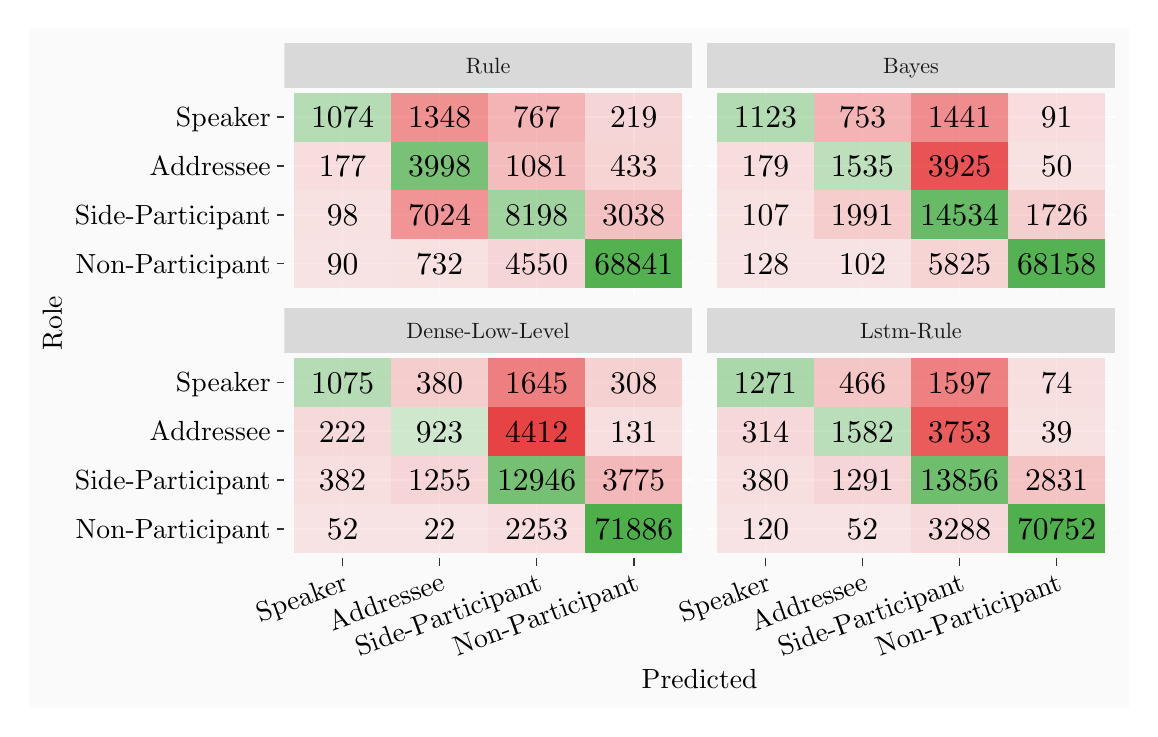
\begin{tikzpicture}[x=1pt,y=1pt]
\definecolor{fillColor}{RGB}{255,255,255}
\path[use as bounding box,fill=fillColor,fill opacity=0.00] (0,0) rectangle (398.34,246.17);
\begin{scope}
\path[clip] (  0.00,  0.00) rectangle (398.34,246.17);
\definecolor{drawColor}{RGB}{255,255,255}
\definecolor{fillColor}{gray}{0.98}

\path[draw=drawColor,line width= 0.6pt,line join=round,line cap=round,fill=fillColor] (  0.00,  0.00) rectangle (398.34,246.17);
\end{scope}
\begin{scope}
\path[clip] ( 92.74,150.34) rectangle (240.04,224.42);
\definecolor{drawColor}{RGB}{255,255,255}

\path[draw=drawColor,line width= 0.6pt,line join=round] ( 92.74,160.93) --
	(240.04,160.93);

\path[draw=drawColor,line width= 0.6pt,line join=round] ( 92.74,178.56) --
	(240.04,178.56);

\path[draw=drawColor,line width= 0.6pt,line join=round] ( 92.74,196.20) --
	(240.04,196.20);

\path[draw=drawColor,line width= 0.6pt,line join=round] ( 92.74,213.84) --
	(240.04,213.84);

\path[draw=drawColor,line width= 0.6pt,line join=round] (113.78,150.34) --
	(113.78,224.42);

\path[draw=drawColor,line width= 0.6pt,line join=round] (148.85,150.34) --
	(148.85,224.42);

\path[draw=drawColor,line width= 0.6pt,line join=round] (183.92,150.34) --
	(183.92,224.42);

\path[draw=drawColor,line width= 0.6pt,line join=round] (218.99,150.34) --
	(218.99,224.42);
\definecolor{fillColor}{RGB}{77,175,74}

\path[fill=fillColor,fill opacity=0.39] ( 96.24,205.02) rectangle (131.32,222.66);
\definecolor{fillColor}{RGB}{228,26,28}

\path[fill=fillColor,fill opacity=0.47] (131.32,205.02) rectangle (166.39,222.66);
\definecolor{fillColor}{RGB}{228,26,28}

\path[fill=fillColor,fill opacity=0.31] (166.39,205.02) rectangle (201.46,222.66);
\definecolor{fillColor}{RGB}{228,26,28}

\path[fill=fillColor,fill opacity=0.16] (201.46,205.02) rectangle (236.53,222.66);
\definecolor{fillColor}{RGB}{228,26,28}

\path[fill=fillColor,fill opacity=0.13] ( 96.24,187.38) rectangle (131.32,205.02);
\definecolor{fillColor}{RGB}{77,175,74}

\path[fill=fillColor,fill opacity=0.75] (131.32,187.38) rectangle (166.39,205.02);
\definecolor{fillColor}{RGB}{228,26,28}

\path[fill=fillColor,fill opacity=0.27] (166.39,187.38) rectangle (201.46,205.02);
\definecolor{fillColor}{RGB}{228,26,28}

\path[fill=fillColor,fill opacity=0.17] (201.46,187.38) rectangle (236.53,205.02);
\definecolor{fillColor}{RGB}{228,26,28}

\path[fill=fillColor,fill opacity=0.11] ( 96.24,169.74) rectangle (131.32,187.38);
\definecolor{fillColor}{RGB}{228,26,28}

\path[fill=fillColor,fill opacity=0.45] (131.32,169.74) rectangle (166.39,187.38);
\definecolor{fillColor}{RGB}{77,175,74}

\path[fill=fillColor,fill opacity=0.51] (166.39,169.74) rectangle (201.46,187.38);
\definecolor{fillColor}{RGB}{228,26,28}

\path[fill=fillColor,fill opacity=0.25] (201.46,169.74) rectangle (236.53,187.38);
\definecolor{fillColor}{RGB}{228,26,28}

\path[fill=fillColor,fill opacity=0.10] ( 96.24,152.11) rectangle (131.32,169.74);
\definecolor{fillColor}{RGB}{228,26,28}

\path[fill=fillColor,fill opacity=0.11] (131.32,152.11) rectangle (166.39,169.74);
\definecolor{fillColor}{RGB}{228,26,28}

\path[fill=fillColor,fill opacity=0.16] (166.39,152.11) rectangle (201.46,169.74);
\definecolor{fillColor}{RGB}{77,175,74}

\path[fill=fillColor,fill opacity=0.96] (201.46,152.11) rectangle (236.53,169.74);
\definecolor{drawColor}{RGB}{0,0,0}

\node[text=drawColor,anchor=base,inner sep=0pt, outer sep=0pt, scale=  1.14] at (113.78,209.92) {1074};

\node[text=drawColor,anchor=base,inner sep=0pt, outer sep=0pt, scale=  1.14] at (148.85,209.92) {1348};

\node[text=drawColor,anchor=base,inner sep=0pt, outer sep=0pt, scale=  1.14] at (183.92,209.92) {767};

\node[text=drawColor,anchor=base,inner sep=0pt, outer sep=0pt, scale=  1.14] at (218.99,209.92) {219};

\node[text=drawColor,anchor=base,inner sep=0pt, outer sep=0pt, scale=  1.14] at (113.78,192.28) {177};

\node[text=drawColor,anchor=base,inner sep=0pt, outer sep=0pt, scale=  1.14] at (148.85,192.28) {3998};

\node[text=drawColor,anchor=base,inner sep=0pt, outer sep=0pt, scale=  1.14] at (183.92,192.28) {1081};

\node[text=drawColor,anchor=base,inner sep=0pt, outer sep=0pt, scale=  1.14] at (218.99,192.28) {433};

\node[text=drawColor,anchor=base,inner sep=0pt, outer sep=0pt, scale=  1.14] at (113.78,174.64) {98};

\node[text=drawColor,anchor=base,inner sep=0pt, outer sep=0pt, scale=  1.14] at (148.85,174.64) {7024};

\node[text=drawColor,anchor=base,inner sep=0pt, outer sep=0pt, scale=  1.14] at (183.92,174.64) {8198};

\node[text=drawColor,anchor=base,inner sep=0pt, outer sep=0pt, scale=  1.14] at (218.99,174.64) {3038};

\node[text=drawColor,anchor=base,inner sep=0pt, outer sep=0pt, scale=  1.14] at (113.78,157.01) {90};

\node[text=drawColor,anchor=base,inner sep=0pt, outer sep=0pt, scale=  1.14] at (148.85,157.01) {732};

\node[text=drawColor,anchor=base,inner sep=0pt, outer sep=0pt, scale=  1.14] at (183.92,157.01) {4550};

\node[text=drawColor,anchor=base,inner sep=0pt, outer sep=0pt, scale=  1.14] at (218.99,157.01) {68841};
\end{scope}
\begin{scope}
\path[clip] ( 92.74, 54.51) rectangle (240.04,128.59);
\definecolor{drawColor}{RGB}{255,255,255}

\path[draw=drawColor,line width= 0.6pt,line join=round] ( 92.74, 65.09) --
	(240.04, 65.09);

\path[draw=drawColor,line width= 0.6pt,line join=round] ( 92.74, 82.73) --
	(240.04, 82.73);

\path[draw=drawColor,line width= 0.6pt,line join=round] ( 92.74,100.37) --
	(240.04,100.37);

\path[draw=drawColor,line width= 0.6pt,line join=round] ( 92.74,118.01) --
	(240.04,118.01);

\path[draw=drawColor,line width= 0.6pt,line join=round] (113.78, 54.51) --
	(113.78,128.59);

\path[draw=drawColor,line width= 0.6pt,line join=round] (148.85, 54.51) --
	(148.85,128.59);

\path[draw=drawColor,line width= 0.6pt,line join=round] (183.92, 54.51) --
	(183.92,128.59);

\path[draw=drawColor,line width= 0.6pt,line join=round] (218.99, 54.51) --
	(218.99,128.59);
\definecolor{fillColor}{RGB}{77,175,74}

\path[fill=fillColor,fill opacity=0.39] ( 96.24,109.19) rectangle (131.32,126.83);
\definecolor{fillColor}{RGB}{228,26,28}

\path[fill=fillColor,fill opacity=0.20] (131.32,109.19) rectangle (166.39,126.83);
\definecolor{fillColor}{RGB}{228,26,28}

\path[fill=fillColor,fill opacity=0.55] (166.39,109.19) rectangle (201.46,126.83);
\definecolor{fillColor}{RGB}{228,26,28}

\path[fill=fillColor,fill opacity=0.18] (201.46,109.19) rectangle (236.53,126.83);
\definecolor{fillColor}{RGB}{228,26,28}

\path[fill=fillColor,fill opacity=0.14] ( 96.24, 91.55) rectangle (131.32,109.19);
\definecolor{fillColor}{RGB}{77,175,74}

\path[fill=fillColor,fill opacity=0.25] (131.32, 91.55) rectangle (166.39,109.19);
\definecolor{fillColor}{RGB}{228,26,28}

\path[fill=fillColor,fill opacity=0.82] (166.39, 91.55) rectangle (201.46,109.19);
\definecolor{fillColor}{RGB}{228,26,28}

\path[fill=fillColor,fill opacity=0.12] (201.46, 91.55) rectangle (236.53,109.19);
\definecolor{fillColor}{RGB}{228,26,28}

\path[fill=fillColor,fill opacity=0.12] ( 96.24, 73.91) rectangle (131.32, 91.55);
\definecolor{fillColor}{RGB}{228,26,28}

\path[fill=fillColor,fill opacity=0.16] (131.32, 73.91) rectangle (166.39, 91.55);
\definecolor{fillColor}{RGB}{77,175,74}

\path[fill=fillColor,fill opacity=0.76] (166.39, 73.91) rectangle (201.46, 91.55);
\definecolor{fillColor}{RGB}{228,26,28}

\path[fill=fillColor,fill opacity=0.29] (201.46, 73.91) rectangle (236.53, 91.55);
\definecolor{fillColor}{RGB}{228,26,28}

\path[fill=fillColor,fill opacity=0.10] ( 96.24, 56.28) rectangle (131.32, 73.91);

\path[fill=fillColor,fill opacity=0.10] (131.32, 56.28) rectangle (166.39, 73.91);
\definecolor{fillColor}{RGB}{228,26,28}

\path[fill=fillColor,fill opacity=0.13] (166.39, 56.28) rectangle (201.46, 73.91);
\definecolor{fillColor}{RGB}{77,175,74}

\path[fill=fillColor] (201.46, 56.28) rectangle (236.53, 73.91);
\definecolor{drawColor}{RGB}{0,0,0}

\node[text=drawColor,anchor=base,inner sep=0pt, outer sep=0pt, scale=  1.14] at (113.78,114.09) {1075};

\node[text=drawColor,anchor=base,inner sep=0pt, outer sep=0pt, scale=  1.14] at (148.85,114.09) {380};

\node[text=drawColor,anchor=base,inner sep=0pt, outer sep=0pt, scale=  1.14] at (183.92,114.09) {1645};

\node[text=drawColor,anchor=base,inner sep=0pt, outer sep=0pt, scale=  1.14] at (218.99,114.09) {308};

\node[text=drawColor,anchor=base,inner sep=0pt, outer sep=0pt, scale=  1.14] at (113.78, 96.45) {222};

\node[text=drawColor,anchor=base,inner sep=0pt, outer sep=0pt, scale=  1.14] at (148.85, 96.45) {923};

\node[text=drawColor,anchor=base,inner sep=0pt, outer sep=0pt, scale=  1.14] at (183.92, 96.45) {4412};

\node[text=drawColor,anchor=base,inner sep=0pt, outer sep=0pt, scale=  1.14] at (218.99, 96.45) {131};

\node[text=drawColor,anchor=base,inner sep=0pt, outer sep=0pt, scale=  1.14] at (113.78, 78.81) {382};

\node[text=drawColor,anchor=base,inner sep=0pt, outer sep=0pt, scale=  1.14] at (148.85, 78.81) {1255};

\node[text=drawColor,anchor=base,inner sep=0pt, outer sep=0pt, scale=  1.14] at (183.92, 78.81) {12946};

\node[text=drawColor,anchor=base,inner sep=0pt, outer sep=0pt, scale=  1.14] at (218.99, 78.81) {3775};

\node[text=drawColor,anchor=base,inner sep=0pt, outer sep=0pt, scale=  1.14] at (113.78, 61.18) {52};

\node[text=drawColor,anchor=base,inner sep=0pt, outer sep=0pt, scale=  1.14] at (148.85, 61.18) {22};

\node[text=drawColor,anchor=base,inner sep=0pt, outer sep=0pt, scale=  1.14] at (183.92, 61.18) {2253};

\node[text=drawColor,anchor=base,inner sep=0pt, outer sep=0pt, scale=  1.14] at (218.99, 61.18) {71886};
\end{scope}
\begin{scope}
\path[clip] (245.54,150.34) rectangle (392.84,224.42);
\definecolor{drawColor}{RGB}{255,255,255}

\path[draw=drawColor,line width= 0.6pt,line join=round] (245.54,160.93) --
	(392.84,160.93);

\path[draw=drawColor,line width= 0.6pt,line join=round] (245.54,178.56) --
	(392.84,178.56);

\path[draw=drawColor,line width= 0.6pt,line join=round] (245.54,196.20) --
	(392.84,196.20);

\path[draw=drawColor,line width= 0.6pt,line join=round] (245.54,213.84) --
	(392.84,213.84);

\path[draw=drawColor,line width= 0.6pt,line join=round] (266.58,150.34) --
	(266.58,224.42);

\path[draw=drawColor,line width= 0.6pt,line join=round] (301.65,150.34) --
	(301.65,224.42);

\path[draw=drawColor,line width= 0.6pt,line join=round] (336.72,150.34) --
	(336.72,224.42);

\path[draw=drawColor,line width= 0.6pt,line join=round] (371.80,150.34) --
	(371.80,224.42);
\definecolor{fillColor}{RGB}{77,175,74}

\path[fill=fillColor,fill opacity=0.41] (249.04,205.02) rectangle (284.12,222.66);
\definecolor{fillColor}{RGB}{228,26,28}

\path[fill=fillColor,fill opacity=0.31] (284.12,205.02) rectangle (319.19,222.66);
\definecolor{fillColor}{RGB}{228,26,28}

\path[fill=fillColor,fill opacity=0.49] (319.19,205.02) rectangle (354.26,222.66);
\definecolor{fillColor}{RGB}{228,26,28}

\path[fill=fillColor,fill opacity=0.13] (354.26,205.02) rectangle (389.33,222.66);
\definecolor{fillColor}{RGB}{228,26,28}

\path[fill=fillColor,fill opacity=0.13] (249.04,187.38) rectangle (284.12,205.02);
\definecolor{fillColor}{RGB}{77,175,74}

\path[fill=fillColor,fill opacity=0.35] (284.12,187.38) rectangle (319.19,205.02);
\definecolor{fillColor}{RGB}{228,26,28}

\path[fill=fillColor,fill opacity=0.74] (319.19,187.38) rectangle (354.26,205.02);
\definecolor{fillColor}{RGB}{228,26,28}

\path[fill=fillColor,fill opacity=0.11] (354.26,187.38) rectangle (389.33,205.02);
\definecolor{fillColor}{RGB}{228,26,28}

\path[fill=fillColor,fill opacity=0.11] (249.04,169.74) rectangle (284.12,187.38);
\definecolor{fillColor}{RGB}{228,26,28}

\path[fill=fillColor,fill opacity=0.20] (284.12,169.74) rectangle (319.19,187.38);
\definecolor{fillColor}{RGB}{77,175,74}

\path[fill=fillColor,fill opacity=0.84] (319.19,169.74) rectangle (354.26,187.38);
\definecolor{fillColor}{RGB}{228,26,28}

\path[fill=fillColor,fill opacity=0.19] (354.26,169.74) rectangle (389.33,187.38);
\definecolor{fillColor}{RGB}{228,26,28}

\path[fill=fillColor,fill opacity=0.10] (249.04,152.11) rectangle (284.12,169.74);

\path[fill=fillColor,fill opacity=0.10] (284.12,152.11) rectangle (319.19,169.74);
\definecolor{fillColor}{RGB}{228,26,28}

\path[fill=fillColor,fill opacity=0.17] (319.19,152.11) rectangle (354.26,169.74);
\definecolor{fillColor}{RGB}{77,175,74}

\path[fill=fillColor,fill opacity=0.95] (354.26,152.11) rectangle (389.33,169.74);
\definecolor{drawColor}{RGB}{0,0,0}

\node[text=drawColor,anchor=base,inner sep=0pt, outer sep=0pt, scale=  1.14] at (266.58,209.92) {1123};

\node[text=drawColor,anchor=base,inner sep=0pt, outer sep=0pt, scale=  1.14] at (301.65,209.92) {753};

\node[text=drawColor,anchor=base,inner sep=0pt, outer sep=0pt, scale=  1.14] at (336.72,209.92) {1441};

\node[text=drawColor,anchor=base,inner sep=0pt, outer sep=0pt, scale=  1.14] at (371.80,209.92) {91};

\node[text=drawColor,anchor=base,inner sep=0pt, outer sep=0pt, scale=  1.14] at (266.58,192.28) {179};

\node[text=drawColor,anchor=base,inner sep=0pt, outer sep=0pt, scale=  1.14] at (301.65,192.28) {1535};

\node[text=drawColor,anchor=base,inner sep=0pt, outer sep=0pt, scale=  1.14] at (336.72,192.28) {3925};

\node[text=drawColor,anchor=base,inner sep=0pt, outer sep=0pt, scale=  1.14] at (371.80,192.28) {50};

\node[text=drawColor,anchor=base,inner sep=0pt, outer sep=0pt, scale=  1.14] at (266.58,174.64) {107};

\node[text=drawColor,anchor=base,inner sep=0pt, outer sep=0pt, scale=  1.14] at (301.65,174.64) {1991};

\node[text=drawColor,anchor=base,inner sep=0pt, outer sep=0pt, scale=  1.14] at (336.72,174.64) {14534};

\node[text=drawColor,anchor=base,inner sep=0pt, outer sep=0pt, scale=  1.14] at (371.80,174.64) {1726};

\node[text=drawColor,anchor=base,inner sep=0pt, outer sep=0pt, scale=  1.14] at (266.58,157.01) {128};

\node[text=drawColor,anchor=base,inner sep=0pt, outer sep=0pt, scale=  1.14] at (301.65,157.01) {102};

\node[text=drawColor,anchor=base,inner sep=0pt, outer sep=0pt, scale=  1.14] at (336.72,157.01) {5825};

\node[text=drawColor,anchor=base,inner sep=0pt, outer sep=0pt, scale=  1.14] at (371.80,157.01) {68158};
\end{scope}
\begin{scope}
\path[clip] (245.54, 54.51) rectangle (392.84,128.59);
\definecolor{drawColor}{RGB}{255,255,255}

\path[draw=drawColor,line width= 0.6pt,line join=round] (245.54, 65.09) --
	(392.84, 65.09);

\path[draw=drawColor,line width= 0.6pt,line join=round] (245.54, 82.73) --
	(392.84, 82.73);

\path[draw=drawColor,line width= 0.6pt,line join=round] (245.54,100.37) --
	(392.84,100.37);

\path[draw=drawColor,line width= 0.6pt,line join=round] (245.54,118.01) --
	(392.84,118.01);

\path[draw=drawColor,line width= 0.6pt,line join=round] (266.58, 54.51) --
	(266.58,128.59);

\path[draw=drawColor,line width= 0.6pt,line join=round] (301.65, 54.51) --
	(301.65,128.59);

\path[draw=drawColor,line width= 0.6pt,line join=round] (336.72, 54.51) --
	(336.72,128.59);

\path[draw=drawColor,line width= 0.6pt,line join=round] (371.80, 54.51) --
	(371.80,128.59);
\definecolor{fillColor}{RGB}{77,175,74}

\path[fill=fillColor,fill opacity=0.45] (249.04,109.19) rectangle (284.12,126.83);
\definecolor{fillColor}{RGB}{228,26,28}

\path[fill=fillColor,fill opacity=0.23] (284.12,109.19) rectangle (319.19,126.83);
\definecolor{fillColor}{RGB}{228,26,28}

\path[fill=fillColor,fill opacity=0.54] (319.19,109.19) rectangle (354.26,126.83);
\definecolor{fillColor}{RGB}{228,26,28}

\path[fill=fillColor,fill opacity=0.12] (354.26,109.19) rectangle (389.33,126.83);
\definecolor{fillColor}{RGB}{228,26,28}

\path[fill=fillColor,fill opacity=0.15] (249.04, 91.55) rectangle (284.12,109.19);
\definecolor{fillColor}{RGB}{77,175,74}

\path[fill=fillColor,fill opacity=0.36] (284.12, 91.55) rectangle (319.19,109.19);
\definecolor{fillColor}{RGB}{228,26,28}

\path[fill=fillColor,fill opacity=0.71] (319.19, 91.55) rectangle (354.26,109.19);
\definecolor{fillColor}{RGB}{228,26,28}

\path[fill=fillColor,fill opacity=0.11] (354.26, 91.55) rectangle (389.33,109.19);
\definecolor{fillColor}{RGB}{228,26,28}

\path[fill=fillColor,fill opacity=0.12] (249.04, 73.91) rectangle (284.12, 91.55);
\definecolor{fillColor}{RGB}{228,26,28}

\path[fill=fillColor,fill opacity=0.16] (284.12, 73.91) rectangle (319.19, 91.55);
\definecolor{fillColor}{RGB}{77,175,74}

\path[fill=fillColor,fill opacity=0.80] (319.19, 73.91) rectangle (354.26, 91.55);
\definecolor{fillColor}{RGB}{228,26,28}

\path[fill=fillColor,fill opacity=0.24] (354.26, 73.91) rectangle (389.33, 91.55);
\definecolor{fillColor}{RGB}{228,26,28}

\path[fill=fillColor,fill opacity=0.10] (249.04, 56.28) rectangle (284.12, 73.91);

\path[fill=fillColor,fill opacity=0.10] (284.12, 56.28) rectangle (319.19, 73.91);
\definecolor{fillColor}{RGB}{228,26,28}

\path[fill=fillColor,fill opacity=0.14] (319.19, 56.28) rectangle (354.26, 73.91);
\definecolor{fillColor}{RGB}{77,175,74}

\path[fill=fillColor,fill opacity=0.98] (354.26, 56.28) rectangle (389.33, 73.91);
\definecolor{drawColor}{RGB}{0,0,0}

\node[text=drawColor,anchor=base,inner sep=0pt, outer sep=0pt, scale=  1.14] at (266.58,114.09) {1271};

\node[text=drawColor,anchor=base,inner sep=0pt, outer sep=0pt, scale=  1.14] at (301.65,114.09) {466};

\node[text=drawColor,anchor=base,inner sep=0pt, outer sep=0pt, scale=  1.14] at (336.72,114.09) {1597};

\node[text=drawColor,anchor=base,inner sep=0pt, outer sep=0pt, scale=  1.14] at (371.80,114.09) {74};

\node[text=drawColor,anchor=base,inner sep=0pt, outer sep=0pt, scale=  1.14] at (266.58, 96.45) {314};

\node[text=drawColor,anchor=base,inner sep=0pt, outer sep=0pt, scale=  1.14] at (301.65, 96.45) {1582};

\node[text=drawColor,anchor=base,inner sep=0pt, outer sep=0pt, scale=  1.14] at (336.72, 96.45) {3753};

\node[text=drawColor,anchor=base,inner sep=0pt, outer sep=0pt, scale=  1.14] at (371.80, 96.45) {39};

\node[text=drawColor,anchor=base,inner sep=0pt, outer sep=0pt, scale=  1.14] at (266.58, 78.81) {380};

\node[text=drawColor,anchor=base,inner sep=0pt, outer sep=0pt, scale=  1.14] at (301.65, 78.81) {1291};

\node[text=drawColor,anchor=base,inner sep=0pt, outer sep=0pt, scale=  1.14] at (336.72, 78.81) {13856};

\node[text=drawColor,anchor=base,inner sep=0pt, outer sep=0pt, scale=  1.14] at (371.80, 78.81) {2831};

\node[text=drawColor,anchor=base,inner sep=0pt, outer sep=0pt, scale=  1.14] at (266.58, 61.18) {120};

\node[text=drawColor,anchor=base,inner sep=0pt, outer sep=0pt, scale=  1.14] at (301.65, 61.18) {52};

\node[text=drawColor,anchor=base,inner sep=0pt, outer sep=0pt, scale=  1.14] at (336.72, 61.18) {3288};

\node[text=drawColor,anchor=base,inner sep=0pt, outer sep=0pt, scale=  1.14] at (371.80, 61.18) {70752};
\end{scope}
\begin{scope}
\path[clip] ( 92.74,128.59) rectangle (240.04,144.84);
\definecolor{fillColor}{gray}{0.85}

\path[fill=fillColor] ( 92.74,128.59) rectangle (240.04,144.84);
\definecolor{drawColor}{gray}{0.10}

\node[text=drawColor,anchor=base,inner sep=0pt, outer sep=0pt, scale=  0.80] at (166.39,133.96) {Dense-Low-Level};
\end{scope}
\begin{scope}
\path[clip] (245.54,128.59) rectangle (392.84,144.84);
\definecolor{fillColor}{gray}{0.85}

\path[fill=fillColor] (245.54,128.59) rectangle (392.84,144.84);
\definecolor{drawColor}{gray}{0.10}

\node[text=drawColor,anchor=base,inner sep=0pt, outer sep=0pt, scale=  0.80] at (319.19,133.96) {Lstm-Rule};
\end{scope}
\begin{scope}
\path[clip] ( 92.74,224.42) rectangle (240.04,240.67);
\definecolor{fillColor}{gray}{0.85}

\path[fill=fillColor] ( 92.74,224.42) rectangle (240.04,240.67);
\definecolor{drawColor}{gray}{0.10}

\node[text=drawColor,anchor=base,inner sep=0pt, outer sep=0pt, scale=  0.80] at (166.39,229.79) {Rule};
\end{scope}
\begin{scope}
\path[clip] (245.54,224.42) rectangle (392.84,240.67);
\definecolor{fillColor}{gray}{0.85}

\path[fill=fillColor] (245.54,224.42) rectangle (392.84,240.67);
\definecolor{drawColor}{gray}{0.10}

\node[text=drawColor,anchor=base,inner sep=0pt, outer sep=0pt, scale=  0.80] at (319.19,229.79) {Bayes};
\end{scope}
\begin{scope}
\path[clip] (  0.00,  0.00) rectangle (398.34,246.17);
\definecolor{drawColor}{gray}{0.20}

\path[draw=drawColor,line width= 0.6pt,line join=round] (113.78, 51.76) --
	(113.78, 54.51);

\path[draw=drawColor,line width= 0.6pt,line join=round] (148.85, 51.76) --
	(148.85, 54.51);

\path[draw=drawColor,line width= 0.6pt,line join=round] (183.92, 51.76) --
	(183.92, 54.51);

\path[draw=drawColor,line width= 0.6pt,line join=round] (218.99, 51.76) --
	(218.99, 54.51);
\end{scope}
\begin{scope}
\path[clip] (  0.00,  0.00) rectangle (398.34,246.17);
\definecolor{drawColor}{RGB}{0,0,0}

\node[text=drawColor,rotate= 20.00,anchor=base east,inner sep=0pt, outer sep=0pt, scale=  1.00] at (116.13, 43.09) {Speaker};

\node[text=drawColor,rotate= 20.00,anchor=base east,inner sep=0pt, outer sep=0pt, scale=  1.00] at (151.21, 43.09) {Addressee};

\node[text=drawColor,rotate= 20.00,anchor=base east,inner sep=0pt, outer sep=0pt, scale=  1.00] at (186.28, 43.09) {Side-Participant};

\node[text=drawColor,rotate= 20.00,anchor=base east,inner sep=0pt, outer sep=0pt, scale=  1.00] at (221.35, 43.09) {Non-Participant};
\end{scope}
\begin{scope}
\path[clip] (  0.00,  0.00) rectangle (398.34,246.17);
\definecolor{drawColor}{gray}{0.20}

\path[draw=drawColor,line width= 0.6pt,line join=round] (266.58, 51.76) --
	(266.58, 54.51);

\path[draw=drawColor,line width= 0.6pt,line join=round] (301.65, 51.76) --
	(301.65, 54.51);

\path[draw=drawColor,line width= 0.6pt,line join=round] (336.72, 51.76) --
	(336.72, 54.51);

\path[draw=drawColor,line width= 0.6pt,line join=round] (371.80, 51.76) --
	(371.80, 54.51);
\end{scope}
\begin{scope}
\path[clip] (  0.00,  0.00) rectangle (398.34,246.17);
\definecolor{drawColor}{RGB}{0,0,0}

\node[text=drawColor,rotate= 20.00,anchor=base east,inner sep=0pt, outer sep=0pt, scale=  1.00] at (268.94, 43.09) {Speaker};

\node[text=drawColor,rotate= 20.00,anchor=base east,inner sep=0pt, outer sep=0pt, scale=  1.00] at (304.01, 43.09) {Addressee};

\node[text=drawColor,rotate= 20.00,anchor=base east,inner sep=0pt, outer sep=0pt, scale=  1.00] at (339.08, 43.09) {Side-Participant};

\node[text=drawColor,rotate= 20.00,anchor=base east,inner sep=0pt, outer sep=0pt, scale=  1.00] at (374.15, 43.09) {Non-Participant};
\end{scope}
\begin{scope}
\path[clip] (  0.00,  0.00) rectangle (398.34,246.17);
\definecolor{drawColor}{RGB}{0,0,0}

\node[text=drawColor,anchor=base east,inner sep=0pt, outer sep=0pt, scale=  1.00] at ( 87.79,157.48) {Non-Participant};

\node[text=drawColor,anchor=base east,inner sep=0pt, outer sep=0pt, scale=  1.00] at ( 87.79,175.12) {Side-Participant};

\node[text=drawColor,anchor=base east,inner sep=0pt, outer sep=0pt, scale=  1.00] at ( 87.79,192.76) {Addressee};

\node[text=drawColor,anchor=base east,inner sep=0pt, outer sep=0pt, scale=  1.00] at ( 87.79,210.39) {Speaker};
\end{scope}
\begin{scope}
\path[clip] (  0.00,  0.00) rectangle (398.34,246.17);
\definecolor{drawColor}{gray}{0.20}

\path[draw=drawColor,line width= 0.6pt,line join=round] ( 89.99,160.93) --
	( 92.74,160.93);

\path[draw=drawColor,line width= 0.6pt,line join=round] ( 89.99,178.56) --
	( 92.74,178.56);

\path[draw=drawColor,line width= 0.6pt,line join=round] ( 89.99,196.20) --
	( 92.74,196.20);

\path[draw=drawColor,line width= 0.6pt,line join=round] ( 89.99,213.84) --
	( 92.74,213.84);
\end{scope}
\begin{scope}
\path[clip] (  0.00,  0.00) rectangle (398.34,246.17);
\definecolor{drawColor}{RGB}{0,0,0}

\node[text=drawColor,anchor=base east,inner sep=0pt, outer sep=0pt, scale=  1.00] at ( 87.79, 61.65) {Non-Participant};

\node[text=drawColor,anchor=base east,inner sep=0pt, outer sep=0pt, scale=  1.00] at ( 87.79, 79.29) {Side-Participant};

\node[text=drawColor,anchor=base east,inner sep=0pt, outer sep=0pt, scale=  1.00] at ( 87.79, 96.93) {Addressee};

\node[text=drawColor,anchor=base east,inner sep=0pt, outer sep=0pt, scale=  1.00] at ( 87.79,114.56) {Speaker};
\end{scope}
\begin{scope}
\path[clip] (  0.00,  0.00) rectangle (398.34,246.17);
\definecolor{drawColor}{gray}{0.20}

\path[draw=drawColor,line width= 0.6pt,line join=round] ( 89.99, 65.09) --
	( 92.74, 65.09);

\path[draw=drawColor,line width= 0.6pt,line join=round] ( 89.99, 82.73) --
	( 92.74, 82.73);

\path[draw=drawColor,line width= 0.6pt,line join=round] ( 89.99,100.37) --
	( 92.74,100.37);

\path[draw=drawColor,line width= 0.6pt,line join=round] ( 89.99,118.01) --
	( 92.74,118.01);
\end{scope}
\begin{scope}
\path[clip] (  0.00,  0.00) rectangle (398.34,246.17);
\definecolor{drawColor}{RGB}{0,0,0}

\node[text=drawColor,anchor=base,inner sep=0pt, outer sep=0pt, scale=  1.00] at (242.79,  7.44) {Predicted};
\end{scope}
\begin{scope}
\path[clip] (  0.00,  0.00) rectangle (398.34,246.17);
\definecolor{drawColor}{RGB}{0,0,0}

\node[text=drawColor,rotate= 90.00,anchor=base,inner sep=0pt, outer sep=0pt, scale=  1.00] at ( 12.39,139.47) {Role};
\end{scope}
\end{tikzpicture}

    }
\end{frame}
\begin{frame}{Results - Simple Models}
  \begin{columns}[T] % align columns
    \begin{column}{.7\textwidth}
      \resizebox{1.\textwidth}{!}{%
        \scriptsize
        \begin{tikzpicture}
          \node (b) at (0,0)
          {
            \resizebox{\textwidth}{!}{%
            % Created by tikzDevice version 0.12
% !TEX encoding = UTF-8 Unicode
\begin{tikzpicture}[x=1pt,y=1pt]
\definecolor{fillColor}{RGB}{255,255,255}
\path[use as bounding box,fill=fillColor,fill opacity=0.00] (0,0) rectangle (398.34,246.17);
\begin{scope}
\path[clip] (  0.00, 11.09) rectangle (398.34,235.08);
\definecolor{drawColor}{RGB}{255,255,255}
\definecolor{fillColor}{gray}{0.98}

\path[draw=drawColor,line width= 0.6pt,line join=round,line cap=round,fill=fillColor] (  0.00, 11.09) rectangle (398.34,235.08);
\end{scope}
\begin{scope}
\path[clip] (100.50, 69.36) rectangle (243.92,212.78);
\definecolor{drawColor}{RGB}{255,255,255}

\path[draw=drawColor,line width= 0.6pt,line join=round] (100.50, 89.85) --
	(243.92, 89.85);

\path[draw=drawColor,line width= 0.6pt,line join=round] (100.50,123.99) --
	(243.92,123.99);

\path[draw=drawColor,line width= 0.6pt,line join=round] (100.50,158.14) --
	(243.92,158.14);

\path[draw=drawColor,line width= 0.6pt,line join=round] (100.50,192.29) --
	(243.92,192.29);

\path[draw=drawColor,line width= 0.6pt,line join=round] (120.98, 69.36) --
	(120.98,212.78);

\path[draw=drawColor,line width= 0.6pt,line join=round] (155.13, 69.36) --
	(155.13,212.78);

\path[draw=drawColor,line width= 0.6pt,line join=round] (189.28, 69.36) --
	(189.28,212.78);

\path[draw=drawColor,line width= 0.6pt,line join=round] (223.43, 69.36) --
	(223.43,212.78);
\definecolor{fillColor}{RGB}{77,175,74}

\path[fill=fillColor,fill opacity=0.40] (103.91,175.22) rectangle (138.06,209.36);
\definecolor{fillColor}{RGB}{228,26,28}

\path[fill=fillColor,fill opacity=0.48] (138.06,175.22) rectangle (172.21,209.36);
\definecolor{fillColor}{RGB}{228,26,28}

\path[fill=fillColor,fill opacity=0.32] (172.21,175.22) rectangle (206.35,209.36);
\definecolor{fillColor}{RGB}{228,26,28}

\path[fill=fillColor,fill opacity=0.16] (206.35,175.22) rectangle (240.50,209.36);
\definecolor{fillColor}{RGB}{228,26,28}

\path[fill=fillColor,fill opacity=0.13] (103.91,141.07) rectangle (138.06,175.22);
\definecolor{fillColor}{RGB}{77,175,74}

\path[fill=fillColor,fill opacity=0.78] (138.06,141.07) rectangle (172.21,175.22);
\definecolor{fillColor}{RGB}{228,26,28}

\path[fill=fillColor,fill opacity=0.28] (172.21,141.07) rectangle (206.35,175.22);
\definecolor{fillColor}{RGB}{228,26,28}

\path[fill=fillColor,fill opacity=0.17] (206.35,141.07) rectangle (240.50,175.22);
\definecolor{fillColor}{RGB}{228,26,28}

\path[fill=fillColor,fill opacity=0.11] (103.91,106.92) rectangle (138.06,141.07);
\definecolor{fillColor}{RGB}{228,26,28}

\path[fill=fillColor,fill opacity=0.47] (138.06,106.92) rectangle (172.21,141.07);
\definecolor{fillColor}{RGB}{77,175,74}

\path[fill=fillColor,fill opacity=0.53] (172.21,106.92) rectangle (206.35,141.07);
\definecolor{fillColor}{RGB}{228,26,28}

\path[fill=fillColor,fill opacity=0.26] (206.35,106.92) rectangle (240.50,141.07);
\definecolor{fillColor}{RGB}{228,26,28}

\path[fill=fillColor,fill opacity=0.10] (103.91, 72.77) rectangle (138.06,106.92);
\definecolor{fillColor}{RGB}{228,26,28}

\path[fill=fillColor,fill opacity=0.11] (138.06, 72.77) rectangle (172.21,106.92);
\definecolor{fillColor}{RGB}{228,26,28}

\path[fill=fillColor,fill opacity=0.16] (172.21, 72.77) rectangle (206.35,106.92);
\definecolor{fillColor}{RGB}{77,175,74}

\path[fill=fillColor] (206.35, 72.77) rectangle (240.50,106.92);
\definecolor{drawColor}{RGB}{0,0,0}

\node[text=drawColor,anchor=base,inner sep=0pt, outer sep=0pt, scale=  1.14] at (120.98,188.37) {0.32};

\node[text=drawColor,anchor=base,inner sep=0pt, outer sep=0pt, scale=  1.14] at (155.13,188.37) {0.40};

\node[text=drawColor,anchor=base,inner sep=0pt, outer sep=0pt, scale=  1.14] at (189.28,188.37) {0.23};

\node[text=drawColor,anchor=base,inner sep=0pt, outer sep=0pt, scale=  1.14] at (223.43,188.37) {0.06};

\node[text=drawColor,anchor=base,inner sep=0pt, outer sep=0pt, scale=  1.14] at (120.98,154.22) {0.03};

\node[text=drawColor,anchor=base,inner sep=0pt, outer sep=0pt, scale=  1.14] at (155.13,154.22) {0.70};

\node[text=drawColor,anchor=base,inner sep=0pt, outer sep=0pt, scale=  1.14] at (189.28,154.22) {0.19};

\node[text=drawColor,anchor=base,inner sep=0pt, outer sep=0pt, scale=  1.14] at (223.43,154.22) {0.08};

\node[text=drawColor,anchor=base,inner sep=0pt, outer sep=0pt, scale=  1.14] at (120.98,120.07) {0.01};

\node[text=drawColor,anchor=base,inner sep=0pt, outer sep=0pt, scale=  1.14] at (155.13,120.07) {0.38};

\node[text=drawColor,anchor=base,inner sep=0pt, outer sep=0pt, scale=  1.14] at (189.28,120.07) {0.45};

\node[text=drawColor,anchor=base,inner sep=0pt, outer sep=0pt, scale=  1.14] at (223.43,120.07) {0.17};

\node[text=drawColor,anchor=base,inner sep=0pt, outer sep=0pt, scale=  1.14] at (120.98, 85.93) {0.00};

\node[text=drawColor,anchor=base,inner sep=0pt, outer sep=0pt, scale=  1.14] at (155.13, 85.93) {0.01};

\node[text=drawColor,anchor=base,inner sep=0pt, outer sep=0pt, scale=  1.14] at (189.28, 85.93) {0.06};

\node[text=drawColor,anchor=base,inner sep=0pt, outer sep=0pt, scale=  1.14] at (223.43, 85.93) {0.93};
\end{scope}
\begin{scope}
\path[clip] (249.42, 69.36) rectangle (392.84,212.78);
\definecolor{drawColor}{RGB}{255,255,255}

\path[draw=drawColor,line width= 0.6pt,line join=round] (249.42, 89.85) --
	(392.84, 89.85);

\path[draw=drawColor,line width= 0.6pt,line join=round] (249.42,123.99) --
	(392.84,123.99);

\path[draw=drawColor,line width= 0.6pt,line join=round] (249.42,158.14) --
	(392.84,158.14);

\path[draw=drawColor,line width= 0.6pt,line join=round] (249.42,192.29) --
	(392.84,192.29);

\path[draw=drawColor,line width= 0.6pt,line join=round] (269.91, 69.36) --
	(269.91,212.78);

\path[draw=drawColor,line width= 0.6pt,line join=round] (304.05, 69.36) --
	(304.05,212.78);

\path[draw=drawColor,line width= 0.6pt,line join=round] (338.20, 69.36) --
	(338.20,212.78);

\path[draw=drawColor,line width= 0.6pt,line join=round] (372.35, 69.36) --
	(372.35,212.78);
\definecolor{fillColor}{RGB}{77,175,74}

\path[fill=fillColor,fill opacity=0.42] (252.83,175.22) rectangle (286.98,209.36);
\definecolor{fillColor}{RGB}{228,26,28}

\path[fill=fillColor,fill opacity=0.31] (286.98,175.22) rectangle (321.13,209.36);
\definecolor{fillColor}{RGB}{228,26,28}

\path[fill=fillColor,fill opacity=0.51] (321.13,175.22) rectangle (355.28,209.36);
\definecolor{fillColor}{RGB}{228,26,28}

\path[fill=fillColor,fill opacity=0.13] (355.28,175.22) rectangle (389.42,209.36);
\definecolor{fillColor}{RGB}{228,26,28}

\path[fill=fillColor,fill opacity=0.13] (252.83,141.07) rectangle (286.98,175.22);
\definecolor{fillColor}{RGB}{77,175,74}

\path[fill=fillColor,fill opacity=0.36] (286.98,141.07) rectangle (321.13,175.22);
\definecolor{fillColor}{RGB}{228,26,28}

\path[fill=fillColor,fill opacity=0.77] (321.13,141.07) rectangle (355.28,175.22);
\definecolor{fillColor}{RGB}{228,26,28}

\path[fill=fillColor,fill opacity=0.11] (355.28,141.07) rectangle (389.42,175.22);

\path[fill=fillColor,fill opacity=0.11] (252.83,106.92) rectangle (286.98,141.07);
\definecolor{fillColor}{RGB}{228,26,28}

\path[fill=fillColor,fill opacity=0.20] (286.98,106.92) rectangle (321.13,141.07);
\definecolor{fillColor}{RGB}{77,175,74}

\path[fill=fillColor,fill opacity=0.87] (321.13,106.92) rectangle (355.28,141.07);
\definecolor{fillColor}{RGB}{228,26,28}

\path[fill=fillColor,fill opacity=0.19] (355.28,106.92) rectangle (389.42,141.07);
\definecolor{fillColor}{RGB}{228,26,28}

\path[fill=fillColor,fill opacity=0.10] (252.83, 72.77) rectangle (286.98,106.92);

\path[fill=fillColor,fill opacity=0.10] (286.98, 72.77) rectangle (321.13,106.92);
\definecolor{fillColor}{RGB}{228,26,28}

\path[fill=fillColor,fill opacity=0.18] (321.13, 72.77) rectangle (355.28,106.92);
\definecolor{fillColor}{RGB}{77,175,74}

\path[fill=fillColor,fill opacity=0.99] (355.28, 72.77) rectangle (389.42,106.92);
\definecolor{drawColor}{RGB}{0,0,0}

\node[text=drawColor,anchor=base,inner sep=0pt, outer sep=0pt, scale=  1.14] at (269.91,188.37) {0.33};

\node[text=drawColor,anchor=base,inner sep=0pt, outer sep=0pt, scale=  1.14] at (304.05,188.37) {0.22};

\node[text=drawColor,anchor=base,inner sep=0pt, outer sep=0pt, scale=  1.14] at (338.20,188.37) {0.42};

\node[text=drawColor,anchor=base,inner sep=0pt, outer sep=0pt, scale=  1.14] at (372.35,188.37) {0.03};

\node[text=drawColor,anchor=base,inner sep=0pt, outer sep=0pt, scale=  1.14] at (269.91,154.22) {0.03};

\node[text=drawColor,anchor=base,inner sep=0pt, outer sep=0pt, scale=  1.14] at (304.05,154.22) {0.27};

\node[text=drawColor,anchor=base,inner sep=0pt, outer sep=0pt, scale=  1.14] at (338.20,154.22) {0.69};

\node[text=drawColor,anchor=base,inner sep=0pt, outer sep=0pt, scale=  1.14] at (372.35,154.22) {0.01};

\node[text=drawColor,anchor=base,inner sep=0pt, outer sep=0pt, scale=  1.14] at (269.91,120.07) {0.01};

\node[text=drawColor,anchor=base,inner sep=0pt, outer sep=0pt, scale=  1.14] at (304.05,120.07) {0.11};

\node[text=drawColor,anchor=base,inner sep=0pt, outer sep=0pt, scale=  1.14] at (338.20,120.07) {0.79};

\node[text=drawColor,anchor=base,inner sep=0pt, outer sep=0pt, scale=  1.14] at (372.35,120.07) {0.09};

\node[text=drawColor,anchor=base,inner sep=0pt, outer sep=0pt, scale=  1.14] at (269.91, 85.93) {0.00};

\node[text=drawColor,anchor=base,inner sep=0pt, outer sep=0pt, scale=  1.14] at (304.05, 85.93) {0.00};

\node[text=drawColor,anchor=base,inner sep=0pt, outer sep=0pt, scale=  1.14] at (338.20, 85.93) {0.08};

\node[text=drawColor,anchor=base,inner sep=0pt, outer sep=0pt, scale=  1.14] at (372.35, 85.93) {0.92};
\end{scope}
\begin{scope}
\path[clip] (100.50,212.78) rectangle (243.92,229.58);
\definecolor{fillColor}{gray}{0.85}

\path[fill=fillColor] (100.50,212.78) rectangle (243.92,229.58);
\definecolor{drawColor}{gray}{0.10}

\node[text=drawColor,anchor=base,inner sep=0pt, outer sep=0pt, scale=  0.88] at (172.21,218.15) {Rule};
\end{scope}
\begin{scope}
\path[clip] (249.42,212.78) rectangle (392.84,229.58);
\definecolor{fillColor}{gray}{0.85}

\path[fill=fillColor] (249.42,212.78) rectangle (392.84,229.58);
\definecolor{drawColor}{gray}{0.10}

\node[text=drawColor,anchor=base,inner sep=0pt, outer sep=0pt, scale=  0.88] at (321.13,218.15) {Bayes};
\end{scope}
\begin{scope}
\path[clip] (  0.00,  0.00) rectangle (398.34,246.17);
\definecolor{drawColor}{gray}{0.20}

\path[draw=drawColor,line width= 0.6pt,line join=round] (120.98, 66.61) --
	(120.98, 69.36);

\path[draw=drawColor,line width= 0.6pt,line join=round] (155.13, 66.61) --
	(155.13, 69.36);

\path[draw=drawColor,line width= 0.6pt,line join=round] (189.28, 66.61) --
	(189.28, 69.36);

\path[draw=drawColor,line width= 0.6pt,line join=round] (223.43, 66.61) --
	(223.43, 69.36);
\end{scope}
\begin{scope}
\path[clip] (  0.00,  0.00) rectangle (398.34,246.17);
\definecolor{drawColor}{RGB}{0,0,0}

\node[text=drawColor,rotate= 20.00,anchor=base east,inner sep=0pt, outer sep=0pt, scale=  1.10] at (123.58, 57.29) {Speaker};

\node[text=drawColor,rotate= 20.00,anchor=base east,inner sep=0pt, outer sep=0pt, scale=  1.10] at (157.72, 57.29) {Addressee};

\node[text=drawColor,rotate= 20.00,anchor=base east,inner sep=0pt, outer sep=0pt, scale=  1.10] at (191.87, 57.29) {Side-Participant};

\node[text=drawColor,rotate= 20.00,anchor=base east,inner sep=0pt, outer sep=0pt, scale=  1.10] at (226.02, 57.29) {Non-Participant};
\end{scope}
\begin{scope}
\path[clip] (  0.00,  0.00) rectangle (398.34,246.17);
\definecolor{drawColor}{gray}{0.20}

\path[draw=drawColor,line width= 0.6pt,line join=round] (269.91, 66.61) --
	(269.91, 69.36);

\path[draw=drawColor,line width= 0.6pt,line join=round] (304.05, 66.61) --
	(304.05, 69.36);

\path[draw=drawColor,line width= 0.6pt,line join=round] (338.20, 66.61) --
	(338.20, 69.36);

\path[draw=drawColor,line width= 0.6pt,line join=round] (372.35, 66.61) --
	(372.35, 69.36);
\end{scope}
\begin{scope}
\path[clip] (  0.00,  0.00) rectangle (398.34,246.17);
\definecolor{drawColor}{RGB}{0,0,0}

\node[text=drawColor,rotate= 20.00,anchor=base east,inner sep=0pt, outer sep=0pt, scale=  1.10] at (272.50, 57.29) {Speaker};

\node[text=drawColor,rotate= 20.00,anchor=base east,inner sep=0pt, outer sep=0pt, scale=  1.10] at (306.65, 57.29) {Addressee};

\node[text=drawColor,rotate= 20.00,anchor=base east,inner sep=0pt, outer sep=0pt, scale=  1.10] at (340.79, 57.29) {Side-Participant};

\node[text=drawColor,rotate= 20.00,anchor=base east,inner sep=0pt, outer sep=0pt, scale=  1.10] at (374.94, 57.29) {Non-Participant};
\end{scope}
\begin{scope}
\path[clip] (  0.00,  0.00) rectangle (398.34,246.17);
\definecolor{drawColor}{RGB}{0,0,0}

\node[text=drawColor,anchor=base east,inner sep=0pt, outer sep=0pt, scale=  1.10] at ( 95.55, 86.06) {Non-Participant};

\node[text=drawColor,anchor=base east,inner sep=0pt, outer sep=0pt, scale=  1.10] at ( 95.55,120.21) {Side-Participant};

\node[text=drawColor,anchor=base east,inner sep=0pt, outer sep=0pt, scale=  1.10] at ( 95.55,154.35) {Addressee};

\node[text=drawColor,anchor=base east,inner sep=0pt, outer sep=0pt, scale=  1.10] at ( 95.55,188.50) {Speaker};
\end{scope}
\begin{scope}
\path[clip] (  0.00,  0.00) rectangle (398.34,246.17);
\definecolor{drawColor}{gray}{0.20}

\path[draw=drawColor,line width= 0.6pt,line join=round] ( 97.75, 89.85) --
	(100.50, 89.85);

\path[draw=drawColor,line width= 0.6pt,line join=round] ( 97.75,123.99) --
	(100.50,123.99);

\path[draw=drawColor,line width= 0.6pt,line join=round] ( 97.75,158.14) --
	(100.50,158.14);

\path[draw=drawColor,line width= 0.6pt,line join=round] ( 97.75,192.29) --
	(100.50,192.29);
\end{scope}
\begin{scope}
\path[clip] (  0.00,  0.00) rectangle (398.34,246.17);
\definecolor{drawColor}{RGB}{0,0,0}

\node[text=drawColor,anchor=base,inner sep=0pt, outer sep=0pt, scale=  1.10] at (246.67, 18.53) {Predicted};
\end{scope}
\begin{scope}
\path[clip] (  0.00,  0.00) rectangle (398.34,246.17);
\definecolor{drawColor}{RGB}{0,0,0}

\node[text=drawColor,rotate= 90.00,anchor=base,inner sep=0pt, outer sep=0pt, scale=  1.10] at ( 13.08,141.07) {Role};
\end{scope}
\end{tikzpicture}

            }
          };
          \action<1-3>{\filldraw [fill=bgcolorframe, draw=bgcolorframe] (.12\textwidth,-.125\textwidth) rectangle (.48\textwidth,.215\textwidth);}
        \end{tikzpicture}
      }
    \end{column}%
    \begin{column}{.4\textwidth}
      \vspace{10pt}
      \footnotesize
      \begin{itemize}[label=-]
        \item<1->[] Rule Model 
        \item<2-> Non-Participant good
        \item<3-> Bias for \(Addressee\)
      \end{itemize}
      \vspace{5pt}
      \begin{itemize}[label=-]
        \item<4->[] Bayes Model
        \item<4-> Non-Participant good 
        \item<5-> Bias for \(Side\text{-}Participant\)
        \item<6-> \emph{optimal} results
      \end{itemize}
      \vspace{5pt}
      \begin{itemize}[label=-]
        \item<7->[\textcolor{mygreen}{\faCheckCircle}] Simple Models
      \end{itemize}
    \end{column}%
  \end{columns}
\end{frame}
\begin{frame}{Low-Level Features \& Time Sequences}
  \begin{columns}[T] % align columns
    \begin{column}{.25\textwidth}
      \vspace{10pt}
      \centering
      \resizebox{\textwidth}{!}{%
          \scriptsize
          \begin{tikzpicture}
          \node (b) at (0,0)
          {
            \resizebox{1.35\textwidth}{!}{%
            \def\svgwidth{1.3\textwidth}
            \input{generated/nnl-defence-dense.pdf_tex}
            }
          };
          \action<6->{\node (c) at (0,-5)
          {
            \resizebox{1.35\textwidth}{!}{%
            \def\svgwidth{1.3\textwidth}
            \input{generated/nnl-defence-t2.pdf_tex}
            }
          };}
          \action<6->{\node (c) at (0,-5)
          {
            \resizebox{1.35\textwidth}{!}{%
            \def\svgwidth{1.3\textwidth}
            \input{generated/nnl-defence-t1.pdf_tex}
            }
          };}
          \action<6->{\node (c) at (0,-5)
          {
            \resizebox{1.35\textwidth}{!}{%
            \def\svgwidth{1.3\textwidth}
            \input{generated/nnl-defence-lstm.pdf_tex}
            }
          };}
           \end{tikzpicture}
        }
    \end{column}%
    \begin{column}{.75\textwidth}
    \onslide<2->{
\footnotesize\hspace{30pt}
    \begin{itemize}
      \item<2->[]Feature Sets
      \item<3->[\(Rule\)] 4D Binary, same as Bayesian Network
      \item<4->[\(Rule_{raw}\)] 4D Continuous, from underlying cost functions  
      \item<5->[\(full\)] 148D Continuous, Agent ID - Face Keypoints - Number of Persons - Group Position - Group Sub-Costs 
    \end{itemize}
    \vspace{20pt}
    \begin{itemize}
      \item<6->[]Same Feature Sets
      \item<6->[\(time\)] Time Sequences of 15 Observations \(\approx\) \SI{1}{\second}
    \end{itemize}
    }
    \end{column}%
  \end{columns}%
\end{frame}
\begin{frame}{Results - Accuracy \& Mean \(F_1\)}
  \begin{columns}[T] % align columns
    \begin{column}{.55\textwidth}
      \resizebox{1.\textwidth}{!}{%
        \small
        % Created by tikzDevice version 0.12
% !TEX encoding = UTF-8 Unicode
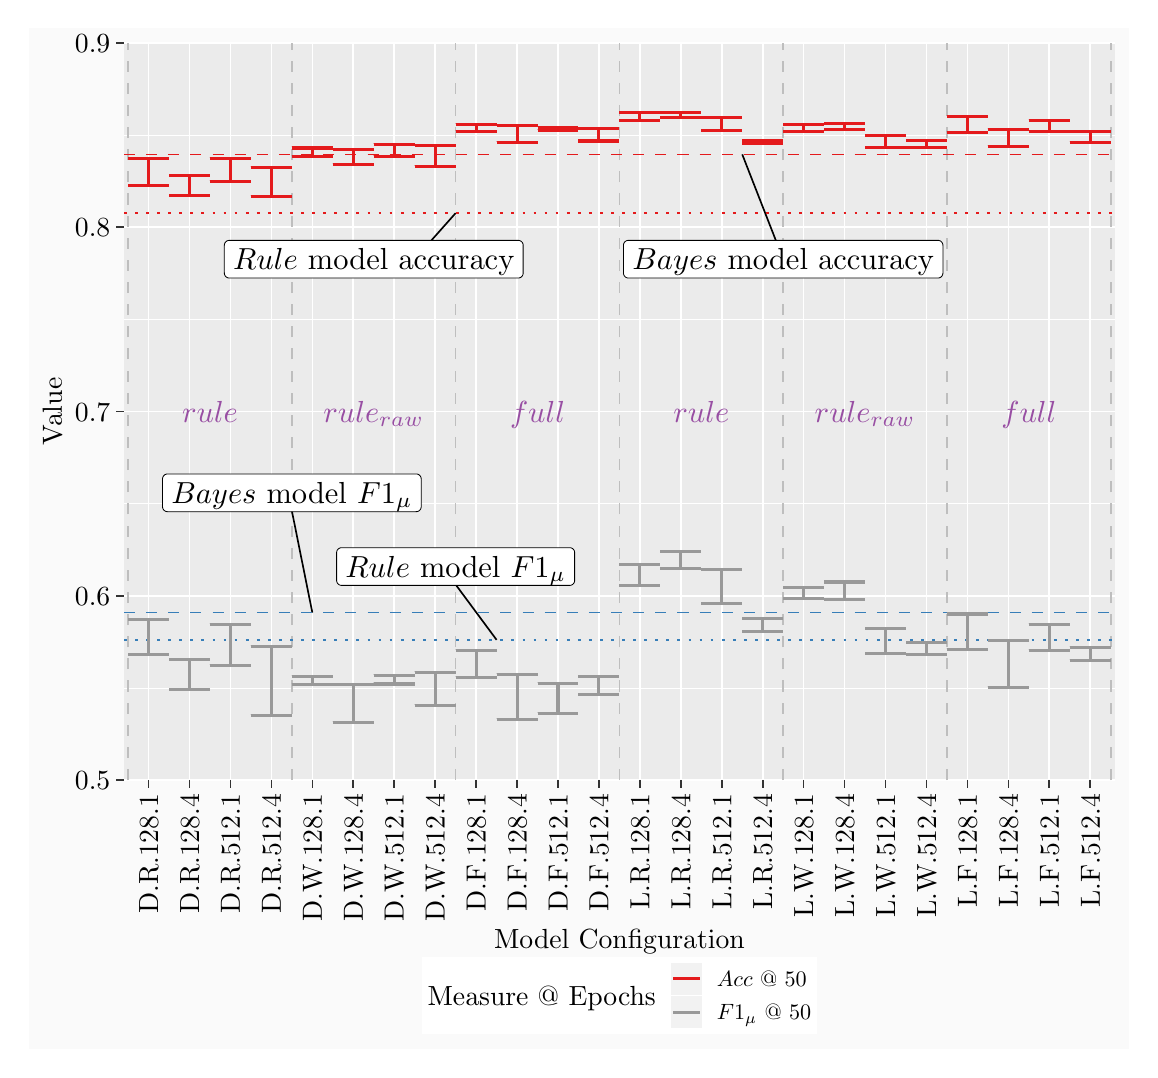
\begin{tikzpicture}[x=1pt,y=1pt]
\definecolor{fillColor}{RGB}{255,255,255}
\path[use as bounding box,fill=fillColor,fill opacity=0.00] (0,0) rectangle (398.34,369.26);
\begin{scope}
\path[clip] (  0.00,  0.00) rectangle (398.34,369.26);
\definecolor{drawColor}{RGB}{255,255,255}
\definecolor{fillColor}{gray}{0.98}

\path[draw=drawColor,line width= 0.6pt,line join=round,line cap=round,fill=fillColor] (  0.00,  0.00) rectangle (398.34,369.26);
\end{scope}
\begin{scope}
\path[clip] ( 34.81, 97.36) rectangle (392.84,363.76);
\definecolor{fillColor}{gray}{0.92}

\path[fill=fillColor] ( 34.81, 97.36) rectangle (392.84,363.76);
\definecolor{drawColor}{RGB}{255,255,255}

\path[draw=drawColor,line width= 0.3pt,line join=round] ( 34.81,130.66) --
	(392.84,130.66);

\path[draw=drawColor,line width= 0.3pt,line join=round] ( 34.81,197.26) --
	(392.84,197.26);

\path[draw=drawColor,line width= 0.3pt,line join=round] ( 34.81,263.86) --
	(392.84,263.86);

\path[draw=drawColor,line width= 0.3pt,line join=round] ( 34.81,330.46) --
	(392.84,330.46);

\path[draw=drawColor,line width= 0.6pt,line join=round] ( 34.81, 97.36) --
	(392.84, 97.36);

\path[draw=drawColor,line width= 0.6pt,line join=round] ( 34.81,163.96) --
	(392.84,163.96);

\path[draw=drawColor,line width= 0.6pt,line join=round] ( 34.81,230.56) --
	(392.84,230.56);

\path[draw=drawColor,line width= 0.6pt,line join=round] ( 34.81,297.16) --
	(392.84,297.16);

\path[draw=drawColor,line width= 0.6pt,line join=round] ( 34.81,363.76) --
	(392.84,363.76);

\path[draw=drawColor,line width= 0.6pt,line join=round] ( 43.68, 97.36) --
	( 43.68,363.76);

\path[draw=drawColor,line width= 0.6pt,line join=round] ( 58.48, 97.36) --
	( 58.48,363.76);

\path[draw=drawColor,line width= 0.6pt,line join=round] ( 73.27, 97.36) --
	( 73.27,363.76);

\path[draw=drawColor,line width= 0.6pt,line join=round] ( 88.07, 97.36) --
	( 88.07,363.76);

\path[draw=drawColor,line width= 0.6pt,line join=round] (102.86, 97.36) --
	(102.86,363.76);

\path[draw=drawColor,line width= 0.6pt,line join=round] (117.66, 97.36) --
	(117.66,363.76);

\path[draw=drawColor,line width= 0.6pt,line join=round] (132.45, 97.36) --
	(132.45,363.76);

\path[draw=drawColor,line width= 0.6pt,line join=round] (147.25, 97.36) --
	(147.25,363.76);

\path[draw=drawColor,line width= 0.6pt,line join=round] (162.04, 97.36) --
	(162.04,363.76);

\path[draw=drawColor,line width= 0.6pt,line join=round] (176.84, 97.36) --
	(176.84,363.76);

\path[draw=drawColor,line width= 0.6pt,line join=round] (191.63, 97.36) --
	(191.63,363.76);

\path[draw=drawColor,line width= 0.6pt,line join=round] (206.42, 97.36) --
	(206.42,363.76);

\path[draw=drawColor,line width= 0.6pt,line join=round] (221.22, 97.36) --
	(221.22,363.76);

\path[draw=drawColor,line width= 0.6pt,line join=round] (236.01, 97.36) --
	(236.01,363.76);

\path[draw=drawColor,line width= 0.6pt,line join=round] (250.81, 97.36) --
	(250.81,363.76);

\path[draw=drawColor,line width= 0.6pt,line join=round] (265.60, 97.36) --
	(265.60,363.76);

\path[draw=drawColor,line width= 0.6pt,line join=round] (280.40, 97.36) --
	(280.40,363.76);

\path[draw=drawColor,line width= 0.6pt,line join=round] (295.19, 97.36) --
	(295.19,363.76);

\path[draw=drawColor,line width= 0.6pt,line join=round] (309.99, 97.36) --
	(309.99,363.76);

\path[draw=drawColor,line width= 0.6pt,line join=round] (324.78, 97.36) --
	(324.78,363.76);

\path[draw=drawColor,line width= 0.6pt,line join=round] (339.58, 97.36) --
	(339.58,363.76);

\path[draw=drawColor,line width= 0.6pt,line join=round] (354.37, 97.36) --
	(354.37,363.76);

\path[draw=drawColor,line width= 0.6pt,line join=round] (369.17, 97.36) --
	(369.17,363.76);

\path[draw=drawColor,line width= 0.6pt,line join=round] (383.96, 97.36) --
	(383.96,363.76);
\definecolor{drawColor}{RGB}{190,190,190}

\path[draw=drawColor,line width= 0.6pt,dash pattern=on 4pt off 4pt ,line join=round] ( 36.29, 97.36) -- ( 36.29,363.76);

\path[draw=drawColor,line width= 0.6pt,dash pattern=on 4pt off 4pt ,line join=round] ( 95.46, 97.36) -- ( 95.46,363.76);

\path[draw=drawColor,line width= 0.6pt,dash pattern=on 4pt off 4pt ,line join=round] (154.64, 97.36) -- (154.64,363.76);

\path[draw=drawColor,line width= 0.6pt,dash pattern=on 4pt off 4pt ,line join=round] (213.82, 97.36) -- (213.82,363.76);

\path[draw=drawColor,line width= 0.6pt,dash pattern=on 4pt off 4pt ,line join=round] (273.00, 97.36) -- (273.00,363.76);

\path[draw=drawColor,line width= 0.6pt,dash pattern=on 4pt off 4pt ,line join=round] (332.18, 97.36) -- (332.18,363.76);

\path[draw=drawColor,line width= 0.6pt,dash pattern=on 4pt off 4pt ,line join=round] (391.36, 97.36) -- (391.36,363.76);
\definecolor{drawColor}{RGB}{152,78,163}

\node[text=drawColor,anchor=base,inner sep=0pt, outer sep=0pt, scale=  1.10] at ( 65.87,226.76) {\(rule\)};

\node[text=drawColor,anchor=base,inner sep=0pt, outer sep=0pt, scale=  1.10] at (125.05,226.76) {\(rule_{raw}\)};

\node[text=drawColor,anchor=base,inner sep=0pt, outer sep=0pt, scale=  1.10] at (184.23,226.76) {\(full\)};

\node[text=drawColor,anchor=base,inner sep=0pt, outer sep=0pt, scale=  1.10] at (243.41,226.76) {\(rule\)};

\node[text=drawColor,anchor=base,inner sep=0pt, outer sep=0pt, scale=  1.10] at (302.59,226.76) {\(rule_{raw}\)};

\node[text=drawColor,anchor=base,inner sep=0pt, outer sep=0pt, scale=  1.10] at (361.77,226.76) {\(full\)};
\definecolor{drawColor}{RGB}{0,0,0}

\path[draw=drawColor,line width= 0.6pt,line join=round] (139.85,285.60) --
	(154.64,302.25);

\path[draw=drawColor,line width= 0.6pt,line join=round] (258.21,323.47) --
	(273.00,285.60);

\path[draw=drawColor,line width= 0.6pt,line join=round] (154.64,168.03) --
	(169.44,148.05);

\path[draw=drawColor,line width= 0.6pt,line join=round] ( 95.46,194.67) --
	(102.86,157.89);
\definecolor{fillColor}{RGB}{255,255,255}

\path[draw=drawColor,line width= 0.3pt,line join=round,line cap=round,fill=fillColor] ( 50.54,194.36) --
	(140.39,194.36) --
	(140.32,194.37) --
	(140.61,194.38) --
	(140.89,194.44) --
	(141.17,194.54) --
	(141.42,194.68) --
	(141.64,194.87) --
	(141.84,195.09) --
	(141.99,195.33) --
	(142.11,195.60) --
	(142.17,195.88) --
	(142.20,196.17) --
	(142.20,196.17) --
	(142.20,206.18) --
	(142.20,206.18) --
	(142.17,206.47) --
	(142.11,206.76) --
	(141.99,207.02) --
	(141.84,207.27) --
	(141.64,207.49) --
	(141.42,207.67) --
	(141.17,207.82) --
	(140.89,207.92) --
	(140.61,207.98) --
	(140.39,207.99) --
	( 50.54,207.99) --
	( 50.75,207.98) --
	( 50.46,207.99) --
	( 50.18,207.95) --
	( 49.90,207.87) --
	( 49.63,207.75) --
	( 49.39,207.58) --
	( 49.18,207.38) --
	( 49.01,207.15) --
	( 48.88,206.89) --
	( 48.78,206.62) --
	( 48.74,206.33) --
	( 48.73,206.18) --
	( 48.73,196.17) --
	( 48.74,196.32) --
	( 48.74,196.03) --
	( 48.78,195.74) --
	( 48.88,195.46) --
	( 49.01,195.21) --
	( 49.18,194.97) --
	( 49.39,194.77) --
	( 49.63,194.61) --
	( 49.90,194.48) --
	( 50.18,194.40) --
	( 50.46,194.37) --
	cycle;
\end{scope}
\begin{scope}
\path[clip] ( 34.81, 97.36) rectangle (392.84,363.76);
\definecolor{drawColor}{RGB}{0,0,0}

\node[text=drawColor,anchor=base,inner sep=0pt, outer sep=0pt, scale=  1.10] at ( 95.46,197.38) {\(Bayes\) model \(F1_\mu\)};
\definecolor{fillColor}{RGB}{255,255,255}

\path[draw=drawColor,line width= 0.3pt,line join=round,line cap=round,fill=fillColor] (113.44,167.72) --
	(195.85,167.72) --
	(195.77,167.73) --
	(196.06,167.74) --
	(196.35,167.80) --
	(196.62,167.90) --
	(196.87,168.04) --
	(197.10,168.23) --
	(197.29,168.45) --
	(197.45,168.69) --
	(197.56,168.96) --
	(197.63,169.24) --
	(197.65,169.53) --
	(197.65,169.53) --
	(197.65,179.54) --
	(197.65,179.54) --
	(197.63,179.83) --
	(197.56,180.12) --
	(197.45,180.38) --
	(197.29,180.63) --
	(197.10,180.85) --
	(196.87,181.03) --
	(196.62,181.18) --
	(196.35,181.28) --
	(196.06,181.34) --
	(195.85,181.35) --
	(113.44,181.35) --
	(113.66,181.34) --
	(113.37,181.35) --
	(113.08,181.31) --
	(112.80,181.23) --
	(112.54,181.11) --
	(112.30,180.94) --
	(112.09,180.74) --
	(111.91,180.51) --
	(111.78,180.25) --
	(111.69,179.98) --
	(111.64,179.69) --
	(111.63,179.54) --
	(111.63,169.53) --
	(111.64,169.68) --
	(111.64,169.39) --
	(111.69,169.10) --
	(111.78,168.82) --
	(111.91,168.57) --
	(112.09,168.33) --
	(112.30,168.13) --
	(112.54,167.97) --
	(112.80,167.84) --
	(113.08,167.76) --
	(113.37,167.73) --
	cycle;
\end{scope}
\begin{scope}
\path[clip] ( 34.81, 97.36) rectangle (392.84,363.76);
\definecolor{drawColor}{RGB}{0,0,0}

\node[text=drawColor,anchor=base,inner sep=0pt, outer sep=0pt, scale=  1.10] at (154.64,170.74) {\(Rule\) model \(F1_\mu\)};
\definecolor{fillColor}{RGB}{255,255,255}

\path[draw=drawColor,line width= 0.3pt,line join=round,line cap=round,fill=fillColor] ( 72.87,278.78) --
	(177.24,278.78) --
	(177.16,278.79) --
	(177.46,278.80) --
	(177.74,278.86) --
	(178.01,278.96) --
	(178.26,279.10) --
	(178.49,279.29) --
	(178.68,279.51) --
	(178.84,279.75) --
	(178.95,280.02) --
	(179.02,280.30) --
	(179.04,280.59) --
	(179.04,280.59) --
	(179.04,290.60) --
	(179.04,290.60) --
	(179.02,290.89) --
	(178.95,291.18) --
	(178.84,291.44) --
	(178.68,291.69) --
	(178.49,291.91) --
	(178.26,292.09) --
	(178.01,292.24) --
	(177.74,292.34) --
	(177.46,292.40) --
	(177.24,292.41) --
	( 72.87,292.41) --
	( 73.09,292.40) --
	( 72.80,292.41) --
	( 72.51,292.37) --
	( 72.23,292.29) --
	( 71.97,292.17) --
	( 71.73,292.00) --
	( 71.52,291.80) --
	( 71.34,291.57) --
	( 71.21,291.31) --
	( 71.12,291.04) --
	( 71.07,290.75) --
	( 71.06,290.60) --
	( 71.06,280.59) --
	( 71.07,280.74) --
	( 71.07,280.45) --
	( 71.12,280.16) --
	( 71.21,279.88) --
	( 71.34,279.63) --
	( 71.52,279.39) --
	( 71.73,279.19) --
	( 71.97,279.03) --
	( 72.23,278.90) --
	( 72.51,278.82) --
	( 72.80,278.79) --
	cycle;
\end{scope}
\begin{scope}
\path[clip] ( 34.81, 97.36) rectangle (392.84,363.76);
\definecolor{drawColor}{RGB}{0,0,0}

\node[text=drawColor,anchor=base,inner sep=0pt, outer sep=0pt, scale=  1.10] at (125.05,281.80) {\(Rule\) model accuracy};
\definecolor{fillColor}{RGB}{255,255,255}

\path[draw=drawColor,line width= 0.3pt,line join=round,line cap=round,fill=fillColor] (217.09,278.78) --
	(328.91,278.78) --
	(328.84,278.79) --
	(329.13,278.80) --
	(329.41,278.86) --
	(329.68,278.96) --
	(329.94,279.10) --
	(330.16,279.29) --
	(330.35,279.51) --
	(330.51,279.75) --
	(330.62,280.02) --
	(330.69,280.30) --
	(330.72,280.59) --
	(330.72,280.59) --
	(330.72,290.60) --
	(330.72,290.60) --
	(330.69,290.89) --
	(330.62,291.18) --
	(330.51,291.44) --
	(330.35,291.69) --
	(330.16,291.91) --
	(329.94,292.09) --
	(329.68,292.24) --
	(329.41,292.34) --
	(329.13,292.40) --
	(328.91,292.41) --
	(217.09,292.41) --
	(217.31,292.40) --
	(217.02,292.41) --
	(216.73,292.37) --
	(216.45,292.29) --
	(216.19,292.17) --
	(215.95,292.00) --
	(215.74,291.80) --
	(215.57,291.57) --
	(215.43,291.31) --
	(215.34,291.04) --
	(215.29,290.75) --
	(215.29,290.60) --
	(215.29,280.59) --
	(215.29,280.74) --
	(215.29,280.45) --
	(215.34,280.16) --
	(215.43,279.88) --
	(215.57,279.63) --
	(215.74,279.39) --
	(215.95,279.19) --
	(216.19,279.03) --
	(216.45,278.90) --
	(216.73,278.82) --
	(217.02,278.79) --
	cycle;
\end{scope}
\begin{scope}
\path[clip] ( 34.81, 97.36) rectangle (392.84,363.76);
\definecolor{drawColor}{RGB}{0,0,0}

\node[text=drawColor,anchor=base,inner sep=0pt, outer sep=0pt, scale=  1.10] at (273.00,281.80) {\(Bayes\) model accuracy};
\definecolor{drawColor}{RGB}{228,26,28}

\path[draw=drawColor,line width= 0.6pt,dash pattern=on 4pt off 4pt ,line join=round] ( 34.81,323.47) -- (392.84,323.47);

\path[draw=drawColor,line width= 0.6pt,dash pattern=on 1pt off 3pt ,line join=round] ( 34.81,302.25) -- (392.84,302.25);
\definecolor{drawColor}{RGB}{55,126,184}

\path[draw=drawColor,line width= 0.6pt,dash pattern=on 4pt off 4pt ,line join=round] ( 34.81,157.89) -- (392.84,157.89);

\path[draw=drawColor,line width= 0.6pt,dash pattern=on 1pt off 3pt ,line join=round] ( 34.81,148.05) -- (392.84,148.05);
\definecolor{drawColor}{RGB}{228,26,28}

\path[draw=drawColor,line width= 1.1pt,line join=round] ( 36.29,322.01) --
	( 51.08,322.01);

\path[draw=drawColor,line width= 1.1pt,line join=round] ( 43.68,322.01) --
	( 43.68,312.38);

\path[draw=drawColor,line width= 1.1pt,line join=round] ( 36.29,312.38) --
	( 51.08,312.38);

\path[draw=drawColor,line width= 1.1pt,line join=round] ( 36.29,322.01) --
	( 51.08,322.01);

\path[draw=drawColor,line width= 1.1pt,line join=round] ( 43.68,322.01) --
	( 43.68,312.38);

\path[draw=drawColor,line width= 1.1pt,line join=round] ( 36.29,312.38) --
	( 51.08,312.38);

\path[draw=drawColor,line width= 1.1pt,line join=round] ( 36.29,322.01) --
	( 51.08,322.01);

\path[draw=drawColor,line width= 1.1pt,line join=round] ( 43.68,322.01) --
	( 43.68,312.38);

\path[draw=drawColor,line width= 1.1pt,line join=round] ( 36.29,312.38) --
	( 51.08,312.38);

\path[draw=drawColor,line width= 1.1pt,line join=round] ( 36.29,322.01) --
	( 51.08,322.01);

\path[draw=drawColor,line width= 1.1pt,line join=round] ( 43.68,322.01) --
	( 43.68,312.38);

\path[draw=drawColor,line width= 1.1pt,line join=round] ( 36.29,312.38) --
	( 51.08,312.38);

\path[draw=drawColor,line width= 1.1pt,line join=round] ( 36.29,322.01) --
	( 51.08,322.01);

\path[draw=drawColor,line width= 1.1pt,line join=round] ( 43.68,322.01) --
	( 43.68,312.38);

\path[draw=drawColor,line width= 1.1pt,line join=round] ( 36.29,312.38) --
	( 51.08,312.38);

\path[draw=drawColor,line width= 1.1pt,line join=round] ( 36.29,322.01) --
	( 51.08,322.01);

\path[draw=drawColor,line width= 1.1pt,line join=round] ( 43.68,322.01) --
	( 43.68,312.38);

\path[draw=drawColor,line width= 1.1pt,line join=round] ( 36.29,312.38) --
	( 51.08,312.38);

\path[draw=drawColor,line width= 1.1pt,line join=round] ( 36.29,322.01) --
	( 51.08,322.01);

\path[draw=drawColor,line width= 1.1pt,line join=round] ( 43.68,322.01) --
	( 43.68,312.38);

\path[draw=drawColor,line width= 1.1pt,line join=round] ( 36.29,312.38) --
	( 51.08,312.38);

\path[draw=drawColor,line width= 1.1pt,line join=round] ( 36.29,322.01) --
	( 51.08,322.01);

\path[draw=drawColor,line width= 1.1pt,line join=round] ( 43.68,322.01) --
	( 43.68,312.38);

\path[draw=drawColor,line width= 1.1pt,line join=round] ( 36.29,312.38) --
	( 51.08,312.38);

\path[draw=drawColor,line width= 1.1pt,line join=round] ( 51.08,315.99) --
	( 65.87,315.99);

\path[draw=drawColor,line width= 1.1pt,line join=round] ( 58.48,315.99) --
	( 58.48,308.46);

\path[draw=drawColor,line width= 1.1pt,line join=round] ( 51.08,308.46) --
	( 65.87,308.46);

\path[draw=drawColor,line width= 1.1pt,line join=round] ( 51.08,315.99) --
	( 65.87,315.99);

\path[draw=drawColor,line width= 1.1pt,line join=round] ( 58.48,315.99) --
	( 58.48,308.46);

\path[draw=drawColor,line width= 1.1pt,line join=round] ( 51.08,308.46) --
	( 65.87,308.46);

\path[draw=drawColor,line width= 1.1pt,line join=round] ( 51.08,315.99) --
	( 65.87,315.99);

\path[draw=drawColor,line width= 1.1pt,line join=round] ( 58.48,315.99) --
	( 58.48,308.46);

\path[draw=drawColor,line width= 1.1pt,line join=round] ( 51.08,308.46) --
	( 65.87,308.46);

\path[draw=drawColor,line width= 1.1pt,line join=round] ( 51.08,315.99) --
	( 65.87,315.99);

\path[draw=drawColor,line width= 1.1pt,line join=round] ( 58.48,315.99) --
	( 58.48,308.46);

\path[draw=drawColor,line width= 1.1pt,line join=round] ( 51.08,308.46) --
	( 65.87,308.46);

\path[draw=drawColor,line width= 1.1pt,line join=round] ( 51.08,315.99) --
	( 65.87,315.99);

\path[draw=drawColor,line width= 1.1pt,line join=round] ( 58.48,315.99) --
	( 58.48,308.46);

\path[draw=drawColor,line width= 1.1pt,line join=round] ( 51.08,308.46) --
	( 65.87,308.46);

\path[draw=drawColor,line width= 1.1pt,line join=round] ( 51.08,315.99) --
	( 65.87,315.99);

\path[draw=drawColor,line width= 1.1pt,line join=round] ( 58.48,315.99) --
	( 58.48,308.46);

\path[draw=drawColor,line width= 1.1pt,line join=round] ( 51.08,308.46) --
	( 65.87,308.46);

\path[draw=drawColor,line width= 1.1pt,line join=round] ( 51.08,315.99) --
	( 65.87,315.99);

\path[draw=drawColor,line width= 1.1pt,line join=round] ( 58.48,315.99) --
	( 58.48,308.46);

\path[draw=drawColor,line width= 1.1pt,line join=round] ( 51.08,308.46) --
	( 65.87,308.46);

\path[draw=drawColor,line width= 1.1pt,line join=round] ( 51.08,315.99) --
	( 65.87,315.99);

\path[draw=drawColor,line width= 1.1pt,line join=round] ( 58.48,315.99) --
	( 58.48,308.46);

\path[draw=drawColor,line width= 1.1pt,line join=round] ( 51.08,308.46) --
	( 65.87,308.46);

\path[draw=drawColor,line width= 1.1pt,line join=round] ( 65.87,321.85) --
	( 80.67,321.85);

\path[draw=drawColor,line width= 1.1pt,line join=round] ( 73.27,321.85) --
	( 73.27,313.84);

\path[draw=drawColor,line width= 1.1pt,line join=round] ( 65.87,313.84) --
	( 80.67,313.84);

\path[draw=drawColor,line width= 1.1pt,line join=round] ( 65.87,321.85) --
	( 80.67,321.85);

\path[draw=drawColor,line width= 1.1pt,line join=round] ( 73.27,321.85) --
	( 73.27,313.84);

\path[draw=drawColor,line width= 1.1pt,line join=round] ( 65.87,313.84) --
	( 80.67,313.84);

\path[draw=drawColor,line width= 1.1pt,line join=round] ( 65.87,321.85) --
	( 80.67,321.85);

\path[draw=drawColor,line width= 1.1pt,line join=round] ( 73.27,321.85) --
	( 73.27,313.84);

\path[draw=drawColor,line width= 1.1pt,line join=round] ( 65.87,313.84) --
	( 80.67,313.84);

\path[draw=drawColor,line width= 1.1pt,line join=round] ( 65.87,321.85) --
	( 80.67,321.85);

\path[draw=drawColor,line width= 1.1pt,line join=round] ( 73.27,321.85) --
	( 73.27,313.84);

\path[draw=drawColor,line width= 1.1pt,line join=round] ( 65.87,313.84) --
	( 80.67,313.84);

\path[draw=drawColor,line width= 1.1pt,line join=round] ( 65.87,321.85) --
	( 80.67,321.85);

\path[draw=drawColor,line width= 1.1pt,line join=round] ( 73.27,321.85) --
	( 73.27,313.84);

\path[draw=drawColor,line width= 1.1pt,line join=round] ( 65.87,313.84) --
	( 80.67,313.84);

\path[draw=drawColor,line width= 1.1pt,line join=round] ( 65.87,321.85) --
	( 80.67,321.85);

\path[draw=drawColor,line width= 1.1pt,line join=round] ( 73.27,321.85) --
	( 73.27,313.84);

\path[draw=drawColor,line width= 1.1pt,line join=round] ( 65.87,313.84) --
	( 80.67,313.84);

\path[draw=drawColor,line width= 1.1pt,line join=round] ( 65.87,321.85) --
	( 80.67,321.85);

\path[draw=drawColor,line width= 1.1pt,line join=round] ( 73.27,321.85) --
	( 73.27,313.84);

\path[draw=drawColor,line width= 1.1pt,line join=round] ( 65.87,313.84) --
	( 80.67,313.84);

\path[draw=drawColor,line width= 1.1pt,line join=round] ( 65.87,321.85) --
	( 80.67,321.85);

\path[draw=drawColor,line width= 1.1pt,line join=round] ( 73.27,321.85) --
	( 73.27,313.84);

\path[draw=drawColor,line width= 1.1pt,line join=round] ( 65.87,313.84) --
	( 80.67,313.84);

\path[draw=drawColor,line width= 1.1pt,line join=round] ( 80.67,318.63) --
	( 95.46,318.63);

\path[draw=drawColor,line width= 1.1pt,line join=round] ( 88.07,318.63) --
	( 88.07,308.32);

\path[draw=drawColor,line width= 1.1pt,line join=round] ( 80.67,308.32) --
	( 95.46,308.32);

\path[draw=drawColor,line width= 1.1pt,line join=round] ( 80.67,318.63) --
	( 95.46,318.63);

\path[draw=drawColor,line width= 1.1pt,line join=round] ( 88.07,318.63) --
	( 88.07,308.32);

\path[draw=drawColor,line width= 1.1pt,line join=round] ( 80.67,308.32) --
	( 95.46,308.32);

\path[draw=drawColor,line width= 1.1pt,line join=round] ( 80.67,318.63) --
	( 95.46,318.63);

\path[draw=drawColor,line width= 1.1pt,line join=round] ( 88.07,318.63) --
	( 88.07,308.32);

\path[draw=drawColor,line width= 1.1pt,line join=round] ( 80.67,308.32) --
	( 95.46,308.32);

\path[draw=drawColor,line width= 1.1pt,line join=round] ( 80.67,318.63) --
	( 95.46,318.63);

\path[draw=drawColor,line width= 1.1pt,line join=round] ( 88.07,318.63) --
	( 88.07,308.32);

\path[draw=drawColor,line width= 1.1pt,line join=round] ( 80.67,308.32) --
	( 95.46,308.32);

\path[draw=drawColor,line width= 1.1pt,line join=round] ( 80.67,318.63) --
	( 95.46,318.63);

\path[draw=drawColor,line width= 1.1pt,line join=round] ( 88.07,318.63) --
	( 88.07,308.32);

\path[draw=drawColor,line width= 1.1pt,line join=round] ( 80.67,308.32) --
	( 95.46,308.32);

\path[draw=drawColor,line width= 1.1pt,line join=round] ( 80.67,318.63) --
	( 95.46,318.63);

\path[draw=drawColor,line width= 1.1pt,line join=round] ( 88.07,318.63) --
	( 88.07,308.32);

\path[draw=drawColor,line width= 1.1pt,line join=round] ( 80.67,308.32) --
	( 95.46,308.32);

\path[draw=drawColor,line width= 1.1pt,line join=round] ( 80.67,318.63) --
	( 95.46,318.63);

\path[draw=drawColor,line width= 1.1pt,line join=round] ( 88.07,318.63) --
	( 88.07,308.32);

\path[draw=drawColor,line width= 1.1pt,line join=round] ( 80.67,308.32) --
	( 95.46,308.32);

\path[draw=drawColor,line width= 1.1pt,line join=round] ( 80.67,318.63) --
	( 95.46,318.63);

\path[draw=drawColor,line width= 1.1pt,line join=round] ( 88.07,318.63) --
	( 88.07,308.32);

\path[draw=drawColor,line width= 1.1pt,line join=round] ( 80.67,308.32) --
	( 95.46,308.32);

\path[draw=drawColor,line width= 1.1pt,line join=round] ( 95.46,325.77) --
	(110.26,325.77);

\path[draw=drawColor,line width= 1.1pt,line join=round] (102.86,325.77) --
	(102.86,322.62);

\path[draw=drawColor,line width= 1.1pt,line join=round] ( 95.46,322.62) --
	(110.26,322.62);

\path[draw=drawColor,line width= 1.1pt,line join=round] ( 95.46,325.77) --
	(110.26,325.77);

\path[draw=drawColor,line width= 1.1pt,line join=round] (102.86,325.77) --
	(102.86,322.62);

\path[draw=drawColor,line width= 1.1pt,line join=round] ( 95.46,322.62) --
	(110.26,322.62);

\path[draw=drawColor,line width= 1.1pt,line join=round] ( 95.46,325.77) --
	(110.26,325.77);

\path[draw=drawColor,line width= 1.1pt,line join=round] (102.86,325.77) --
	(102.86,322.62);

\path[draw=drawColor,line width= 1.1pt,line join=round] ( 95.46,322.62) --
	(110.26,322.62);

\path[draw=drawColor,line width= 1.1pt,line join=round] ( 95.46,325.77) --
	(110.26,325.77);

\path[draw=drawColor,line width= 1.1pt,line join=round] (102.86,325.77) --
	(102.86,322.62);

\path[draw=drawColor,line width= 1.1pt,line join=round] ( 95.46,322.62) --
	(110.26,322.62);

\path[draw=drawColor,line width= 1.1pt,line join=round] ( 95.46,325.77) --
	(110.26,325.77);

\path[draw=drawColor,line width= 1.1pt,line join=round] (102.86,325.77) --
	(102.86,322.62);

\path[draw=drawColor,line width= 1.1pt,line join=round] ( 95.46,322.62) --
	(110.26,322.62);

\path[draw=drawColor,line width= 1.1pt,line join=round] ( 95.46,325.77) --
	(110.26,325.77);

\path[draw=drawColor,line width= 1.1pt,line join=round] (102.86,325.77) --
	(102.86,322.62);

\path[draw=drawColor,line width= 1.1pt,line join=round] ( 95.46,322.62) --
	(110.26,322.62);

\path[draw=drawColor,line width= 1.1pt,line join=round] ( 95.46,325.77) --
	(110.26,325.77);

\path[draw=drawColor,line width= 1.1pt,line join=round] (102.86,325.77) --
	(102.86,322.62);

\path[draw=drawColor,line width= 1.1pt,line join=round] ( 95.46,322.62) --
	(110.26,322.62);

\path[draw=drawColor,line width= 1.1pt,line join=round] ( 95.46,325.77) --
	(110.26,325.77);

\path[draw=drawColor,line width= 1.1pt,line join=round] (102.86,325.77) --
	(102.86,322.62);

\path[draw=drawColor,line width= 1.1pt,line join=round] ( 95.46,322.62) --
	(110.26,322.62);

\path[draw=drawColor,line width= 1.1pt,line join=round] (110.26,325.18) --
	(125.05,325.18);

\path[draw=drawColor,line width= 1.1pt,line join=round] (117.66,325.18) --
	(117.66,319.90);

\path[draw=drawColor,line width= 1.1pt,line join=round] (110.26,319.90) --
	(125.05,319.90);

\path[draw=drawColor,line width= 1.1pt,line join=round] (110.26,325.18) --
	(125.05,325.18);

\path[draw=drawColor,line width= 1.1pt,line join=round] (117.66,325.18) --
	(117.66,319.90);

\path[draw=drawColor,line width= 1.1pt,line join=round] (110.26,319.90) --
	(125.05,319.90);

\path[draw=drawColor,line width= 1.1pt,line join=round] (110.26,325.18) --
	(125.05,325.18);

\path[draw=drawColor,line width= 1.1pt,line join=round] (117.66,325.18) --
	(117.66,319.90);

\path[draw=drawColor,line width= 1.1pt,line join=round] (110.26,319.90) --
	(125.05,319.90);

\path[draw=drawColor,line width= 1.1pt,line join=round] (110.26,325.18) --
	(125.05,325.18);

\path[draw=drawColor,line width= 1.1pt,line join=round] (117.66,325.18) --
	(117.66,319.90);

\path[draw=drawColor,line width= 1.1pt,line join=round] (110.26,319.90) --
	(125.05,319.90);

\path[draw=drawColor,line width= 1.1pt,line join=round] (110.26,325.18) --
	(125.05,325.18);

\path[draw=drawColor,line width= 1.1pt,line join=round] (117.66,325.18) --
	(117.66,319.90);

\path[draw=drawColor,line width= 1.1pt,line join=round] (110.26,319.90) --
	(125.05,319.90);

\path[draw=drawColor,line width= 1.1pt,line join=round] (110.26,325.18) --
	(125.05,325.18);

\path[draw=drawColor,line width= 1.1pt,line join=round] (117.66,325.18) --
	(117.66,319.90);

\path[draw=drawColor,line width= 1.1pt,line join=round] (110.26,319.90) --
	(125.05,319.90);

\path[draw=drawColor,line width= 1.1pt,line join=round] (110.26,325.18) --
	(125.05,325.18);

\path[draw=drawColor,line width= 1.1pt,line join=round] (117.66,325.18) --
	(117.66,319.90);

\path[draw=drawColor,line width= 1.1pt,line join=round] (110.26,319.90) --
	(125.05,319.90);

\path[draw=drawColor,line width= 1.1pt,line join=round] (110.26,325.18) --
	(125.05,325.18);

\path[draw=drawColor,line width= 1.1pt,line join=round] (117.66,325.18) --
	(117.66,319.90);

\path[draw=drawColor,line width= 1.1pt,line join=round] (110.26,319.90) --
	(125.05,319.90);

\path[draw=drawColor,line width= 1.1pt,line join=round] (125.05,326.90) --
	(139.85,326.90);

\path[draw=drawColor,line width= 1.1pt,line join=round] (132.45,326.90) --
	(132.45,322.60);

\path[draw=drawColor,line width= 1.1pt,line join=round] (125.05,322.60) --
	(139.85,322.60);

\path[draw=drawColor,line width= 1.1pt,line join=round] (125.05,326.90) --
	(139.85,326.90);

\path[draw=drawColor,line width= 1.1pt,line join=round] (132.45,326.90) --
	(132.45,322.60);

\path[draw=drawColor,line width= 1.1pt,line join=round] (125.05,322.60) --
	(139.85,322.60);

\path[draw=drawColor,line width= 1.1pt,line join=round] (125.05,326.90) --
	(139.85,326.90);

\path[draw=drawColor,line width= 1.1pt,line join=round] (132.45,326.90) --
	(132.45,322.60);

\path[draw=drawColor,line width= 1.1pt,line join=round] (125.05,322.60) --
	(139.85,322.60);

\path[draw=drawColor,line width= 1.1pt,line join=round] (125.05,326.90) --
	(139.85,326.90);

\path[draw=drawColor,line width= 1.1pt,line join=round] (132.45,326.90) --
	(132.45,322.60);

\path[draw=drawColor,line width= 1.1pt,line join=round] (125.05,322.60) --
	(139.85,322.60);

\path[draw=drawColor,line width= 1.1pt,line join=round] (125.05,326.90) --
	(139.85,326.90);

\path[draw=drawColor,line width= 1.1pt,line join=round] (132.45,326.90) --
	(132.45,322.60);

\path[draw=drawColor,line width= 1.1pt,line join=round] (125.05,322.60) --
	(139.85,322.60);

\path[draw=drawColor,line width= 1.1pt,line join=round] (125.05,326.90) --
	(139.85,326.90);

\path[draw=drawColor,line width= 1.1pt,line join=round] (132.45,326.90) --
	(132.45,322.60);

\path[draw=drawColor,line width= 1.1pt,line join=round] (125.05,322.60) --
	(139.85,322.60);

\path[draw=drawColor,line width= 1.1pt,line join=round] (125.05,326.90) --
	(139.85,326.90);

\path[draw=drawColor,line width= 1.1pt,line join=round] (132.45,326.90) --
	(132.45,322.60);

\path[draw=drawColor,line width= 1.1pt,line join=round] (125.05,322.60) --
	(139.85,322.60);

\path[draw=drawColor,line width= 1.1pt,line join=round] (125.05,326.90) --
	(139.85,326.90);

\path[draw=drawColor,line width= 1.1pt,line join=round] (132.45,326.90) --
	(132.45,322.60);

\path[draw=drawColor,line width= 1.1pt,line join=round] (125.05,322.60) --
	(139.85,322.60);

\path[draw=drawColor,line width= 1.1pt,line join=round] (139.85,326.61) --
	(154.64,326.61);

\path[draw=drawColor,line width= 1.1pt,line join=round] (147.25,326.61) --
	(147.25,319.19);

\path[draw=drawColor,line width= 1.1pt,line join=round] (139.85,319.19) --
	(154.64,319.19);

\path[draw=drawColor,line width= 1.1pt,line join=round] (139.85,326.61) --
	(154.64,326.61);

\path[draw=drawColor,line width= 1.1pt,line join=round] (147.25,326.61) --
	(147.25,319.19);

\path[draw=drawColor,line width= 1.1pt,line join=round] (139.85,319.19) --
	(154.64,319.19);

\path[draw=drawColor,line width= 1.1pt,line join=round] (139.85,326.61) --
	(154.64,326.61);

\path[draw=drawColor,line width= 1.1pt,line join=round] (147.25,326.61) --
	(147.25,319.19);

\path[draw=drawColor,line width= 1.1pt,line join=round] (139.85,319.19) --
	(154.64,319.19);

\path[draw=drawColor,line width= 1.1pt,line join=round] (139.85,326.61) --
	(154.64,326.61);

\path[draw=drawColor,line width= 1.1pt,line join=round] (147.25,326.61) --
	(147.25,319.19);

\path[draw=drawColor,line width= 1.1pt,line join=round] (139.85,319.19) --
	(154.64,319.19);

\path[draw=drawColor,line width= 1.1pt,line join=round] (139.85,326.61) --
	(154.64,326.61);

\path[draw=drawColor,line width= 1.1pt,line join=round] (147.25,326.61) --
	(147.25,319.19);

\path[draw=drawColor,line width= 1.1pt,line join=round] (139.85,319.19) --
	(154.64,319.19);

\path[draw=drawColor,line width= 1.1pt,line join=round] (139.85,326.61) --
	(154.64,326.61);

\path[draw=drawColor,line width= 1.1pt,line join=round] (147.25,326.61) --
	(147.25,319.19);

\path[draw=drawColor,line width= 1.1pt,line join=round] (139.85,319.19) --
	(154.64,319.19);

\path[draw=drawColor,line width= 1.1pt,line join=round] (139.85,326.61) --
	(154.64,326.61);

\path[draw=drawColor,line width= 1.1pt,line join=round] (147.25,326.61) --
	(147.25,319.19);

\path[draw=drawColor,line width= 1.1pt,line join=round] (139.85,319.19) --
	(154.64,319.19);

\path[draw=drawColor,line width= 1.1pt,line join=round] (139.85,326.61) --
	(154.64,326.61);

\path[draw=drawColor,line width= 1.1pt,line join=round] (147.25,326.61) --
	(147.25,319.19);

\path[draw=drawColor,line width= 1.1pt,line join=round] (139.85,319.19) --
	(154.64,319.19);

\path[draw=drawColor,line width= 1.1pt,line join=round] (154.64,334.43) --
	(169.44,334.43);

\path[draw=drawColor,line width= 1.1pt,line join=round] (162.04,334.43) --
	(162.04,331.91);

\path[draw=drawColor,line width= 1.1pt,line join=round] (154.64,331.91) --
	(169.44,331.91);

\path[draw=drawColor,line width= 1.1pt,line join=round] (154.64,334.43) --
	(169.44,334.43);

\path[draw=drawColor,line width= 1.1pt,line join=round] (162.04,334.43) --
	(162.04,331.91);

\path[draw=drawColor,line width= 1.1pt,line join=round] (154.64,331.91) --
	(169.44,331.91);

\path[draw=drawColor,line width= 1.1pt,line join=round] (154.64,334.43) --
	(169.44,334.43);

\path[draw=drawColor,line width= 1.1pt,line join=round] (162.04,334.43) --
	(162.04,331.91);

\path[draw=drawColor,line width= 1.1pt,line join=round] (154.64,331.91) --
	(169.44,331.91);

\path[draw=drawColor,line width= 1.1pt,line join=round] (154.64,334.43) --
	(169.44,334.43);

\path[draw=drawColor,line width= 1.1pt,line join=round] (162.04,334.43) --
	(162.04,331.91);

\path[draw=drawColor,line width= 1.1pt,line join=round] (154.64,331.91) --
	(169.44,331.91);

\path[draw=drawColor,line width= 1.1pt,line join=round] (154.64,334.43) --
	(169.44,334.43);

\path[draw=drawColor,line width= 1.1pt,line join=round] (162.04,334.43) --
	(162.04,331.91);

\path[draw=drawColor,line width= 1.1pt,line join=round] (154.64,331.91) --
	(169.44,331.91);

\path[draw=drawColor,line width= 1.1pt,line join=round] (154.64,334.43) --
	(169.44,334.43);

\path[draw=drawColor,line width= 1.1pt,line join=round] (162.04,334.43) --
	(162.04,331.91);

\path[draw=drawColor,line width= 1.1pt,line join=round] (154.64,331.91) --
	(169.44,331.91);

\path[draw=drawColor,line width= 1.1pt,line join=round] (154.64,334.43) --
	(169.44,334.43);

\path[draw=drawColor,line width= 1.1pt,line join=round] (162.04,334.43) --
	(162.04,331.91);

\path[draw=drawColor,line width= 1.1pt,line join=round] (154.64,331.91) --
	(169.44,331.91);

\path[draw=drawColor,line width= 1.1pt,line join=round] (154.64,334.43) --
	(169.44,334.43);

\path[draw=drawColor,line width= 1.1pt,line join=round] (162.04,334.43) --
	(162.04,331.91);

\path[draw=drawColor,line width= 1.1pt,line join=round] (154.64,331.91) --
	(169.44,331.91);

\path[draw=drawColor,line width= 1.1pt,line join=round] (169.44,334.01) --
	(184.23,334.01);

\path[draw=drawColor,line width= 1.1pt,line join=round] (176.84,334.01) --
	(176.84,327.81);

\path[draw=drawColor,line width= 1.1pt,line join=round] (169.44,327.81) --
	(184.23,327.81);

\path[draw=drawColor,line width= 1.1pt,line join=round] (169.44,334.01) --
	(184.23,334.01);

\path[draw=drawColor,line width= 1.1pt,line join=round] (176.84,334.01) --
	(176.84,327.81);

\path[draw=drawColor,line width= 1.1pt,line join=round] (169.44,327.81) --
	(184.23,327.81);

\path[draw=drawColor,line width= 1.1pt,line join=round] (169.44,334.01) --
	(184.23,334.01);

\path[draw=drawColor,line width= 1.1pt,line join=round] (176.84,334.01) --
	(176.84,327.81);

\path[draw=drawColor,line width= 1.1pt,line join=round] (169.44,327.81) --
	(184.23,327.81);

\path[draw=drawColor,line width= 1.1pt,line join=round] (169.44,334.01) --
	(184.23,334.01);

\path[draw=drawColor,line width= 1.1pt,line join=round] (176.84,334.01) --
	(176.84,327.81);

\path[draw=drawColor,line width= 1.1pt,line join=round] (169.44,327.81) --
	(184.23,327.81);

\path[draw=drawColor,line width= 1.1pt,line join=round] (169.44,334.01) --
	(184.23,334.01);

\path[draw=drawColor,line width= 1.1pt,line join=round] (176.84,334.01) --
	(176.84,327.81);

\path[draw=drawColor,line width= 1.1pt,line join=round] (169.44,327.81) --
	(184.23,327.81);

\path[draw=drawColor,line width= 1.1pt,line join=round] (169.44,334.01) --
	(184.23,334.01);

\path[draw=drawColor,line width= 1.1pt,line join=round] (176.84,334.01) --
	(176.84,327.81);

\path[draw=drawColor,line width= 1.1pt,line join=round] (169.44,327.81) --
	(184.23,327.81);

\path[draw=drawColor,line width= 1.1pt,line join=round] (169.44,334.01) --
	(184.23,334.01);

\path[draw=drawColor,line width= 1.1pt,line join=round] (176.84,334.01) --
	(176.84,327.81);

\path[draw=drawColor,line width= 1.1pt,line join=round] (169.44,327.81) --
	(184.23,327.81);

\path[draw=drawColor,line width= 1.1pt,line join=round] (169.44,334.01) --
	(184.23,334.01);

\path[draw=drawColor,line width= 1.1pt,line join=round] (176.84,334.01) --
	(176.84,327.81);

\path[draw=drawColor,line width= 1.1pt,line join=round] (169.44,327.81) --
	(184.23,327.81);

\path[draw=drawColor,line width= 1.1pt,line join=round] (184.23,333.16) --
	(199.03,333.16);

\path[draw=drawColor,line width= 1.1pt,line join=round] (191.63,333.16) --
	(191.63,332.00);

\path[draw=drawColor,line width= 1.1pt,line join=round] (184.23,332.00) --
	(199.03,332.00);

\path[draw=drawColor,line width= 1.1pt,line join=round] (184.23,333.16) --
	(199.03,333.16);

\path[draw=drawColor,line width= 1.1pt,line join=round] (191.63,333.16) --
	(191.63,332.00);

\path[draw=drawColor,line width= 1.1pt,line join=round] (184.23,332.00) --
	(199.03,332.00);

\path[draw=drawColor,line width= 1.1pt,line join=round] (184.23,333.16) --
	(199.03,333.16);

\path[draw=drawColor,line width= 1.1pt,line join=round] (191.63,333.16) --
	(191.63,332.00);

\path[draw=drawColor,line width= 1.1pt,line join=round] (184.23,332.00) --
	(199.03,332.00);

\path[draw=drawColor,line width= 1.1pt,line join=round] (184.23,333.16) --
	(199.03,333.16);

\path[draw=drawColor,line width= 1.1pt,line join=round] (191.63,333.16) --
	(191.63,332.00);

\path[draw=drawColor,line width= 1.1pt,line join=round] (184.23,332.00) --
	(199.03,332.00);

\path[draw=drawColor,line width= 1.1pt,line join=round] (184.23,333.16) --
	(199.03,333.16);

\path[draw=drawColor,line width= 1.1pt,line join=round] (191.63,333.16) --
	(191.63,332.00);

\path[draw=drawColor,line width= 1.1pt,line join=round] (184.23,332.00) --
	(199.03,332.00);

\path[draw=drawColor,line width= 1.1pt,line join=round] (184.23,333.16) --
	(199.03,333.16);

\path[draw=drawColor,line width= 1.1pt,line join=round] (191.63,333.16) --
	(191.63,332.00);

\path[draw=drawColor,line width= 1.1pt,line join=round] (184.23,332.00) --
	(199.03,332.00);

\path[draw=drawColor,line width= 1.1pt,line join=round] (184.23,333.16) --
	(199.03,333.16);

\path[draw=drawColor,line width= 1.1pt,line join=round] (191.63,333.16) --
	(191.63,332.00);

\path[draw=drawColor,line width= 1.1pt,line join=round] (184.23,332.00) --
	(199.03,332.00);

\path[draw=drawColor,line width= 1.1pt,line join=round] (184.23,333.16) --
	(199.03,333.16);

\path[draw=drawColor,line width= 1.1pt,line join=round] (191.63,333.16) --
	(191.63,332.00);

\path[draw=drawColor,line width= 1.1pt,line join=round] (184.23,332.00) --
	(199.03,332.00);

\path[draw=drawColor,line width= 1.1pt,line join=round] (199.03,332.85) --
	(213.82,332.85);

\path[draw=drawColor,line width= 1.1pt,line join=round] (206.42,332.85) --
	(206.42,328.30);

\path[draw=drawColor,line width= 1.1pt,line join=round] (199.03,328.30) --
	(213.82,328.30);

\path[draw=drawColor,line width= 1.1pt,line join=round] (199.03,332.85) --
	(213.82,332.85);

\path[draw=drawColor,line width= 1.1pt,line join=round] (206.42,332.85) --
	(206.42,328.30);

\path[draw=drawColor,line width= 1.1pt,line join=round] (199.03,328.30) --
	(213.82,328.30);

\path[draw=drawColor,line width= 1.1pt,line join=round] (199.03,332.85) --
	(213.82,332.85);

\path[draw=drawColor,line width= 1.1pt,line join=round] (206.42,332.85) --
	(206.42,328.30);

\path[draw=drawColor,line width= 1.1pt,line join=round] (199.03,328.30) --
	(213.82,328.30);

\path[draw=drawColor,line width= 1.1pt,line join=round] (199.03,332.85) --
	(213.82,332.85);

\path[draw=drawColor,line width= 1.1pt,line join=round] (206.42,332.85) --
	(206.42,328.30);

\path[draw=drawColor,line width= 1.1pt,line join=round] (199.03,328.30) --
	(213.82,328.30);

\path[draw=drawColor,line width= 1.1pt,line join=round] (199.03,332.85) --
	(213.82,332.85);

\path[draw=drawColor,line width= 1.1pt,line join=round] (206.42,332.85) --
	(206.42,328.30);

\path[draw=drawColor,line width= 1.1pt,line join=round] (199.03,328.30) --
	(213.82,328.30);

\path[draw=drawColor,line width= 1.1pt,line join=round] (199.03,332.85) --
	(213.82,332.85);

\path[draw=drawColor,line width= 1.1pt,line join=round] (206.42,332.85) --
	(206.42,328.30);

\path[draw=drawColor,line width= 1.1pt,line join=round] (199.03,328.30) --
	(213.82,328.30);

\path[draw=drawColor,line width= 1.1pt,line join=round] (199.03,332.85) --
	(213.82,332.85);

\path[draw=drawColor,line width= 1.1pt,line join=round] (206.42,332.85) --
	(206.42,328.30);

\path[draw=drawColor,line width= 1.1pt,line join=round] (199.03,328.30) --
	(213.82,328.30);

\path[draw=drawColor,line width= 1.1pt,line join=round] (199.03,332.85) --
	(213.82,332.85);

\path[draw=drawColor,line width= 1.1pt,line join=round] (206.42,332.85) --
	(206.42,328.30);

\path[draw=drawColor,line width= 1.1pt,line join=round] (199.03,328.30) --
	(213.82,328.30);

\path[draw=drawColor,line width= 1.1pt,line join=round] (213.82,338.76) --
	(228.62,338.76);

\path[draw=drawColor,line width= 1.1pt,line join=round] (221.22,338.76) --
	(221.22,335.83);

\path[draw=drawColor,line width= 1.1pt,line join=round] (213.82,335.83) --
	(228.62,335.83);

\path[draw=drawColor,line width= 1.1pt,line join=round] (213.82,338.76) --
	(228.62,338.76);

\path[draw=drawColor,line width= 1.1pt,line join=round] (221.22,338.76) --
	(221.22,335.83);

\path[draw=drawColor,line width= 1.1pt,line join=round] (213.82,335.83) --
	(228.62,335.83);

\path[draw=drawColor,line width= 1.1pt,line join=round] (213.82,338.76) --
	(228.62,338.76);

\path[draw=drawColor,line width= 1.1pt,line join=round] (221.22,338.76) --
	(221.22,335.83);

\path[draw=drawColor,line width= 1.1pt,line join=round] (213.82,335.83) --
	(228.62,335.83);

\path[draw=drawColor,line width= 1.1pt,line join=round] (213.82,338.76) --
	(228.62,338.76);

\path[draw=drawColor,line width= 1.1pt,line join=round] (221.22,338.76) --
	(221.22,335.83);

\path[draw=drawColor,line width= 1.1pt,line join=round] (213.82,335.83) --
	(228.62,335.83);

\path[draw=drawColor,line width= 1.1pt,line join=round] (213.82,338.76) --
	(228.62,338.76);

\path[draw=drawColor,line width= 1.1pt,line join=round] (221.22,338.76) --
	(221.22,335.83);

\path[draw=drawColor,line width= 1.1pt,line join=round] (213.82,335.83) --
	(228.62,335.83);

\path[draw=drawColor,line width= 1.1pt,line join=round] (213.82,338.76) --
	(228.62,338.76);

\path[draw=drawColor,line width= 1.1pt,line join=round] (221.22,338.76) --
	(221.22,335.83);

\path[draw=drawColor,line width= 1.1pt,line join=round] (213.82,335.83) --
	(228.62,335.83);

\path[draw=drawColor,line width= 1.1pt,line join=round] (213.82,338.76) --
	(228.62,338.76);

\path[draw=drawColor,line width= 1.1pt,line join=round] (221.22,338.76) --
	(221.22,335.83);

\path[draw=drawColor,line width= 1.1pt,line join=round] (213.82,335.83) --
	(228.62,335.83);

\path[draw=drawColor,line width= 1.1pt,line join=round] (213.82,338.76) --
	(228.62,338.76);

\path[draw=drawColor,line width= 1.1pt,line join=round] (221.22,338.76) --
	(221.22,335.83);

\path[draw=drawColor,line width= 1.1pt,line join=round] (213.82,335.83) --
	(228.62,335.83);

\path[draw=drawColor,line width= 1.1pt,line join=round] (228.62,338.49) --
	(243.41,338.49);

\path[draw=drawColor,line width= 1.1pt,line join=round] (236.01,338.49) --
	(236.01,336.68);

\path[draw=drawColor,line width= 1.1pt,line join=round] (228.62,336.68) --
	(243.41,336.68);

\path[draw=drawColor,line width= 1.1pt,line join=round] (228.62,338.49) --
	(243.41,338.49);

\path[draw=drawColor,line width= 1.1pt,line join=round] (236.01,338.49) --
	(236.01,336.68);

\path[draw=drawColor,line width= 1.1pt,line join=round] (228.62,336.68) --
	(243.41,336.68);

\path[draw=drawColor,line width= 1.1pt,line join=round] (228.62,338.49) --
	(243.41,338.49);

\path[draw=drawColor,line width= 1.1pt,line join=round] (236.01,338.49) --
	(236.01,336.68);

\path[draw=drawColor,line width= 1.1pt,line join=round] (228.62,336.68) --
	(243.41,336.68);

\path[draw=drawColor,line width= 1.1pt,line join=round] (228.62,338.49) --
	(243.41,338.49);

\path[draw=drawColor,line width= 1.1pt,line join=round] (236.01,338.49) --
	(236.01,336.68);

\path[draw=drawColor,line width= 1.1pt,line join=round] (228.62,336.68) --
	(243.41,336.68);

\path[draw=drawColor,line width= 1.1pt,line join=round] (228.62,338.49) --
	(243.41,338.49);

\path[draw=drawColor,line width= 1.1pt,line join=round] (236.01,338.49) --
	(236.01,336.68);

\path[draw=drawColor,line width= 1.1pt,line join=round] (228.62,336.68) --
	(243.41,336.68);

\path[draw=drawColor,line width= 1.1pt,line join=round] (228.62,338.49) --
	(243.41,338.49);

\path[draw=drawColor,line width= 1.1pt,line join=round] (236.01,338.49) --
	(236.01,336.68);

\path[draw=drawColor,line width= 1.1pt,line join=round] (228.62,336.68) --
	(243.41,336.68);

\path[draw=drawColor,line width= 1.1pt,line join=round] (228.62,338.49) --
	(243.41,338.49);

\path[draw=drawColor,line width= 1.1pt,line join=round] (236.01,338.49) --
	(236.01,336.68);

\path[draw=drawColor,line width= 1.1pt,line join=round] (228.62,336.68) --
	(243.41,336.68);

\path[draw=drawColor,line width= 1.1pt,line join=round] (228.62,338.49) --
	(243.41,338.49);

\path[draw=drawColor,line width= 1.1pt,line join=round] (236.01,338.49) --
	(236.01,336.68);

\path[draw=drawColor,line width= 1.1pt,line join=round] (228.62,336.68) --
	(243.41,336.68);

\path[draw=drawColor,line width= 1.1pt,line join=round] (243.41,336.74) --
	(258.21,336.74);

\path[draw=drawColor,line width= 1.1pt,line join=round] (250.81,336.74) --
	(250.81,332.19);

\path[draw=drawColor,line width= 1.1pt,line join=round] (243.41,332.19) --
	(258.21,332.19);

\path[draw=drawColor,line width= 1.1pt,line join=round] (243.41,336.74) --
	(258.21,336.74);

\path[draw=drawColor,line width= 1.1pt,line join=round] (250.81,336.74) --
	(250.81,332.19);

\path[draw=drawColor,line width= 1.1pt,line join=round] (243.41,332.19) --
	(258.21,332.19);

\path[draw=drawColor,line width= 1.1pt,line join=round] (243.41,336.74) --
	(258.21,336.74);

\path[draw=drawColor,line width= 1.1pt,line join=round] (250.81,336.74) --
	(250.81,332.19);

\path[draw=drawColor,line width= 1.1pt,line join=round] (243.41,332.19) --
	(258.21,332.19);

\path[draw=drawColor,line width= 1.1pt,line join=round] (243.41,336.74) --
	(258.21,336.74);

\path[draw=drawColor,line width= 1.1pt,line join=round] (250.81,336.74) --
	(250.81,332.19);

\path[draw=drawColor,line width= 1.1pt,line join=round] (243.41,332.19) --
	(258.21,332.19);

\path[draw=drawColor,line width= 1.1pt,line join=round] (243.41,336.74) --
	(258.21,336.74);

\path[draw=drawColor,line width= 1.1pt,line join=round] (250.81,336.74) --
	(250.81,332.19);

\path[draw=drawColor,line width= 1.1pt,line join=round] (243.41,332.19) --
	(258.21,332.19);

\path[draw=drawColor,line width= 1.1pt,line join=round] (243.41,336.74) --
	(258.21,336.74);

\path[draw=drawColor,line width= 1.1pt,line join=round] (250.81,336.74) --
	(250.81,332.19);

\path[draw=drawColor,line width= 1.1pt,line join=round] (243.41,332.19) --
	(258.21,332.19);

\path[draw=drawColor,line width= 1.1pt,line join=round] (243.41,336.74) --
	(258.21,336.74);

\path[draw=drawColor,line width= 1.1pt,line join=round] (250.81,336.74) --
	(250.81,332.19);

\path[draw=drawColor,line width= 1.1pt,line join=round] (243.41,332.19) --
	(258.21,332.19);

\path[draw=drawColor,line width= 1.1pt,line join=round] (243.41,336.74) --
	(258.21,336.74);

\path[draw=drawColor,line width= 1.1pt,line join=round] (250.81,336.74) --
	(250.81,332.19);

\path[draw=drawColor,line width= 1.1pt,line join=round] (243.41,332.19) --
	(258.21,332.19);

\path[draw=drawColor,line width= 1.1pt,line join=round] (258.21,328.64) --
	(273.00,328.64);

\path[draw=drawColor,line width= 1.1pt,line join=round] (265.60,328.64) --
	(265.60,327.26);

\path[draw=drawColor,line width= 1.1pt,line join=round] (258.21,327.26) --
	(273.00,327.26);

\path[draw=drawColor,line width= 1.1pt,line join=round] (258.21,328.64) --
	(273.00,328.64);

\path[draw=drawColor,line width= 1.1pt,line join=round] (265.60,328.64) --
	(265.60,327.26);

\path[draw=drawColor,line width= 1.1pt,line join=round] (258.21,327.26) --
	(273.00,327.26);

\path[draw=drawColor,line width= 1.1pt,line join=round] (258.21,328.64) --
	(273.00,328.64);

\path[draw=drawColor,line width= 1.1pt,line join=round] (265.60,328.64) --
	(265.60,327.26);

\path[draw=drawColor,line width= 1.1pt,line join=round] (258.21,327.26) --
	(273.00,327.26);

\path[draw=drawColor,line width= 1.1pt,line join=round] (258.21,328.64) --
	(273.00,328.64);

\path[draw=drawColor,line width= 1.1pt,line join=round] (265.60,328.64) --
	(265.60,327.26);

\path[draw=drawColor,line width= 1.1pt,line join=round] (258.21,327.26) --
	(273.00,327.26);

\path[draw=drawColor,line width= 1.1pt,line join=round] (258.21,328.64) --
	(273.00,328.64);

\path[draw=drawColor,line width= 1.1pt,line join=round] (265.60,328.64) --
	(265.60,327.26);

\path[draw=drawColor,line width= 1.1pt,line join=round] (258.21,327.26) --
	(273.00,327.26);

\path[draw=drawColor,line width= 1.1pt,line join=round] (258.21,328.64) --
	(273.00,328.64);

\path[draw=drawColor,line width= 1.1pt,line join=round] (265.60,328.64) --
	(265.60,327.26);

\path[draw=drawColor,line width= 1.1pt,line join=round] (258.21,327.26) --
	(273.00,327.26);

\path[draw=drawColor,line width= 1.1pt,line join=round] (258.21,328.64) --
	(273.00,328.64);

\path[draw=drawColor,line width= 1.1pt,line join=round] (265.60,328.64) --
	(265.60,327.26);

\path[draw=drawColor,line width= 1.1pt,line join=round] (258.21,327.26) --
	(273.00,327.26);

\path[draw=drawColor,line width= 1.1pt,line join=round] (258.21,328.64) --
	(273.00,328.64);

\path[draw=drawColor,line width= 1.1pt,line join=round] (265.60,328.64) --
	(265.60,327.26);

\path[draw=drawColor,line width= 1.1pt,line join=round] (258.21,327.26) --
	(273.00,327.26);

\path[draw=drawColor,line width= 1.1pt,line join=round] (273.00,334.40) --
	(287.80,334.40);

\path[draw=drawColor,line width= 1.1pt,line join=round] (280.40,334.40) --
	(280.40,331.90);

\path[draw=drawColor,line width= 1.1pt,line join=round] (273.00,331.90) --
	(287.80,331.90);

\path[draw=drawColor,line width= 1.1pt,line join=round] (273.00,334.40) --
	(287.80,334.40);

\path[draw=drawColor,line width= 1.1pt,line join=round] (280.40,334.40) --
	(280.40,331.90);

\path[draw=drawColor,line width= 1.1pt,line join=round] (273.00,331.90) --
	(287.80,331.90);

\path[draw=drawColor,line width= 1.1pt,line join=round] (273.00,334.40) --
	(287.80,334.40);

\path[draw=drawColor,line width= 1.1pt,line join=round] (280.40,334.40) --
	(280.40,331.90);

\path[draw=drawColor,line width= 1.1pt,line join=round] (273.00,331.90) --
	(287.80,331.90);

\path[draw=drawColor,line width= 1.1pt,line join=round] (273.00,334.40) --
	(287.80,334.40);

\path[draw=drawColor,line width= 1.1pt,line join=round] (280.40,334.40) --
	(280.40,331.90);

\path[draw=drawColor,line width= 1.1pt,line join=round] (273.00,331.90) --
	(287.80,331.90);

\path[draw=drawColor,line width= 1.1pt,line join=round] (273.00,334.40) --
	(287.80,334.40);

\path[draw=drawColor,line width= 1.1pt,line join=round] (280.40,334.40) --
	(280.40,331.90);

\path[draw=drawColor,line width= 1.1pt,line join=round] (273.00,331.90) --
	(287.80,331.90);

\path[draw=drawColor,line width= 1.1pt,line join=round] (273.00,334.40) --
	(287.80,334.40);

\path[draw=drawColor,line width= 1.1pt,line join=round] (280.40,334.40) --
	(280.40,331.90);

\path[draw=drawColor,line width= 1.1pt,line join=round] (273.00,331.90) --
	(287.80,331.90);

\path[draw=drawColor,line width= 1.1pt,line join=round] (273.00,334.40) --
	(287.80,334.40);

\path[draw=drawColor,line width= 1.1pt,line join=round] (280.40,334.40) --
	(280.40,331.90);

\path[draw=drawColor,line width= 1.1pt,line join=round] (273.00,331.90) --
	(287.80,331.90);

\path[draw=drawColor,line width= 1.1pt,line join=round] (273.00,334.40) --
	(287.80,334.40);

\path[draw=drawColor,line width= 1.1pt,line join=round] (280.40,334.40) --
	(280.40,331.90);

\path[draw=drawColor,line width= 1.1pt,line join=round] (273.00,331.90) --
	(287.80,331.90);

\path[draw=drawColor,line width= 1.1pt,line join=round] (287.80,334.47) --
	(302.59,334.47);

\path[draw=drawColor,line width= 1.1pt,line join=round] (295.19,334.47) --
	(295.19,332.46);

\path[draw=drawColor,line width= 1.1pt,line join=round] (287.80,332.46) --
	(302.59,332.46);

\path[draw=drawColor,line width= 1.1pt,line join=round] (287.80,334.47) --
	(302.59,334.47);

\path[draw=drawColor,line width= 1.1pt,line join=round] (295.19,334.47) --
	(295.19,332.46);

\path[draw=drawColor,line width= 1.1pt,line join=round] (287.80,332.46) --
	(302.59,332.46);

\path[draw=drawColor,line width= 1.1pt,line join=round] (287.80,334.47) --
	(302.59,334.47);

\path[draw=drawColor,line width= 1.1pt,line join=round] (295.19,334.47) --
	(295.19,332.46);

\path[draw=drawColor,line width= 1.1pt,line join=round] (287.80,332.46) --
	(302.59,332.46);

\path[draw=drawColor,line width= 1.1pt,line join=round] (287.80,334.47) --
	(302.59,334.47);

\path[draw=drawColor,line width= 1.1pt,line join=round] (295.19,334.47) --
	(295.19,332.46);

\path[draw=drawColor,line width= 1.1pt,line join=round] (287.80,332.46) --
	(302.59,332.46);

\path[draw=drawColor,line width= 1.1pt,line join=round] (287.80,334.47) --
	(302.59,334.47);

\path[draw=drawColor,line width= 1.1pt,line join=round] (295.19,334.47) --
	(295.19,332.46);

\path[draw=drawColor,line width= 1.1pt,line join=round] (287.80,332.46) --
	(302.59,332.46);

\path[draw=drawColor,line width= 1.1pt,line join=round] (287.80,334.47) --
	(302.59,334.47);

\path[draw=drawColor,line width= 1.1pt,line join=round] (295.19,334.47) --
	(295.19,332.46);

\path[draw=drawColor,line width= 1.1pt,line join=round] (287.80,332.46) --
	(302.59,332.46);

\path[draw=drawColor,line width= 1.1pt,line join=round] (287.80,334.47) --
	(302.59,334.47);

\path[draw=drawColor,line width= 1.1pt,line join=round] (295.19,334.47) --
	(295.19,332.46);

\path[draw=drawColor,line width= 1.1pt,line join=round] (287.80,332.46) --
	(302.59,332.46);

\path[draw=drawColor,line width= 1.1pt,line join=round] (287.80,334.47) --
	(302.59,334.47);

\path[draw=drawColor,line width= 1.1pt,line join=round] (295.19,334.47) --
	(295.19,332.46);

\path[draw=drawColor,line width= 1.1pt,line join=round] (287.80,332.46) --
	(302.59,332.46);

\path[draw=drawColor,line width= 1.1pt,line join=round] (302.59,330.19) --
	(317.39,330.19);

\path[draw=drawColor,line width= 1.1pt,line join=round] (309.99,330.19) --
	(309.99,325.92);

\path[draw=drawColor,line width= 1.1pt,line join=round] (302.59,325.92) --
	(317.39,325.92);

\path[draw=drawColor,line width= 1.1pt,line join=round] (302.59,330.19) --
	(317.39,330.19);

\path[draw=drawColor,line width= 1.1pt,line join=round] (309.99,330.19) --
	(309.99,325.92);

\path[draw=drawColor,line width= 1.1pt,line join=round] (302.59,325.92) --
	(317.39,325.92);

\path[draw=drawColor,line width= 1.1pt,line join=round] (302.59,330.19) --
	(317.39,330.19);

\path[draw=drawColor,line width= 1.1pt,line join=round] (309.99,330.19) --
	(309.99,325.92);

\path[draw=drawColor,line width= 1.1pt,line join=round] (302.59,325.92) --
	(317.39,325.92);

\path[draw=drawColor,line width= 1.1pt,line join=round] (302.59,330.19) --
	(317.39,330.19);

\path[draw=drawColor,line width= 1.1pt,line join=round] (309.99,330.19) --
	(309.99,325.92);

\path[draw=drawColor,line width= 1.1pt,line join=round] (302.59,325.92) --
	(317.39,325.92);

\path[draw=drawColor,line width= 1.1pt,line join=round] (302.59,330.19) --
	(317.39,330.19);

\path[draw=drawColor,line width= 1.1pt,line join=round] (309.99,330.19) --
	(309.99,325.92);

\path[draw=drawColor,line width= 1.1pt,line join=round] (302.59,325.92) --
	(317.39,325.92);

\path[draw=drawColor,line width= 1.1pt,line join=round] (302.59,330.19) --
	(317.39,330.19);

\path[draw=drawColor,line width= 1.1pt,line join=round] (309.99,330.19) --
	(309.99,325.92);

\path[draw=drawColor,line width= 1.1pt,line join=round] (302.59,325.92) --
	(317.39,325.92);

\path[draw=drawColor,line width= 1.1pt,line join=round] (302.59,330.19) --
	(317.39,330.19);

\path[draw=drawColor,line width= 1.1pt,line join=round] (309.99,330.19) --
	(309.99,325.92);

\path[draw=drawColor,line width= 1.1pt,line join=round] (302.59,325.92) --
	(317.39,325.92);

\path[draw=drawColor,line width= 1.1pt,line join=round] (302.59,330.19) --
	(317.39,330.19);

\path[draw=drawColor,line width= 1.1pt,line join=round] (309.99,330.19) --
	(309.99,325.92);

\path[draw=drawColor,line width= 1.1pt,line join=round] (302.59,325.92) --
	(317.39,325.92);

\path[draw=drawColor,line width= 1.1pt,line join=round] (317.39,328.51) --
	(332.18,328.51);

\path[draw=drawColor,line width= 1.1pt,line join=round] (324.78,328.51) --
	(324.78,325.99);

\path[draw=drawColor,line width= 1.1pt,line join=round] (317.39,325.99) --
	(332.18,325.99);

\path[draw=drawColor,line width= 1.1pt,line join=round] (317.39,328.51) --
	(332.18,328.51);

\path[draw=drawColor,line width= 1.1pt,line join=round] (324.78,328.51) --
	(324.78,325.99);

\path[draw=drawColor,line width= 1.1pt,line join=round] (317.39,325.99) --
	(332.18,325.99);

\path[draw=drawColor,line width= 1.1pt,line join=round] (317.39,328.51) --
	(332.18,328.51);

\path[draw=drawColor,line width= 1.1pt,line join=round] (324.78,328.51) --
	(324.78,325.99);

\path[draw=drawColor,line width= 1.1pt,line join=round] (317.39,325.99) --
	(332.18,325.99);

\path[draw=drawColor,line width= 1.1pt,line join=round] (317.39,328.51) --
	(332.18,328.51);

\path[draw=drawColor,line width= 1.1pt,line join=round] (324.78,328.51) --
	(324.78,325.99);

\path[draw=drawColor,line width= 1.1pt,line join=round] (317.39,325.99) --
	(332.18,325.99);

\path[draw=drawColor,line width= 1.1pt,line join=round] (317.39,328.51) --
	(332.18,328.51);

\path[draw=drawColor,line width= 1.1pt,line join=round] (324.78,328.51) --
	(324.78,325.99);

\path[draw=drawColor,line width= 1.1pt,line join=round] (317.39,325.99) --
	(332.18,325.99);

\path[draw=drawColor,line width= 1.1pt,line join=round] (317.39,328.51) --
	(332.18,328.51);

\path[draw=drawColor,line width= 1.1pt,line join=round] (324.78,328.51) --
	(324.78,325.99);

\path[draw=drawColor,line width= 1.1pt,line join=round] (317.39,325.99) --
	(332.18,325.99);

\path[draw=drawColor,line width= 1.1pt,line join=round] (317.39,328.51) --
	(332.18,328.51);

\path[draw=drawColor,line width= 1.1pt,line join=round] (324.78,328.51) --
	(324.78,325.99);

\path[draw=drawColor,line width= 1.1pt,line join=round] (317.39,325.99) --
	(332.18,325.99);

\path[draw=drawColor,line width= 1.1pt,line join=round] (317.39,328.51) --
	(332.18,328.51);

\path[draw=drawColor,line width= 1.1pt,line join=round] (324.78,328.51) --
	(324.78,325.99);

\path[draw=drawColor,line width= 1.1pt,line join=round] (317.39,325.99) --
	(332.18,325.99);

\path[draw=drawColor,line width= 1.1pt,line join=round] (332.18,337.00) --
	(346.97,337.00);

\path[draw=drawColor,line width= 1.1pt,line join=round] (339.58,337.00) --
	(339.58,331.45);

\path[draw=drawColor,line width= 1.1pt,line join=round] (332.18,331.45) --
	(346.97,331.45);

\path[draw=drawColor,line width= 1.1pt,line join=round] (332.18,337.00) --
	(346.97,337.00);

\path[draw=drawColor,line width= 1.1pt,line join=round] (339.58,337.00) --
	(339.58,331.45);

\path[draw=drawColor,line width= 1.1pt,line join=round] (332.18,331.45) --
	(346.97,331.45);

\path[draw=drawColor,line width= 1.1pt,line join=round] (332.18,337.00) --
	(346.97,337.00);

\path[draw=drawColor,line width= 1.1pt,line join=round] (339.58,337.00) --
	(339.58,331.45);

\path[draw=drawColor,line width= 1.1pt,line join=round] (332.18,331.45) --
	(346.97,331.45);

\path[draw=drawColor,line width= 1.1pt,line join=round] (332.18,337.00) --
	(346.97,337.00);

\path[draw=drawColor,line width= 1.1pt,line join=round] (339.58,337.00) --
	(339.58,331.45);

\path[draw=drawColor,line width= 1.1pt,line join=round] (332.18,331.45) --
	(346.97,331.45);

\path[draw=drawColor,line width= 1.1pt,line join=round] (332.18,337.00) --
	(346.97,337.00);

\path[draw=drawColor,line width= 1.1pt,line join=round] (339.58,337.00) --
	(339.58,331.45);

\path[draw=drawColor,line width= 1.1pt,line join=round] (332.18,331.45) --
	(346.97,331.45);

\path[draw=drawColor,line width= 1.1pt,line join=round] (332.18,337.00) --
	(346.97,337.00);

\path[draw=drawColor,line width= 1.1pt,line join=round] (339.58,337.00) --
	(339.58,331.45);

\path[draw=drawColor,line width= 1.1pt,line join=round] (332.18,331.45) --
	(346.97,331.45);

\path[draw=drawColor,line width= 1.1pt,line join=round] (332.18,337.00) --
	(346.97,337.00);

\path[draw=drawColor,line width= 1.1pt,line join=round] (339.58,337.00) --
	(339.58,331.45);

\path[draw=drawColor,line width= 1.1pt,line join=round] (332.18,331.45) --
	(346.97,331.45);

\path[draw=drawColor,line width= 1.1pt,line join=round] (332.18,337.00) --
	(346.97,337.00);

\path[draw=drawColor,line width= 1.1pt,line join=round] (339.58,337.00) --
	(339.58,331.45);

\path[draw=drawColor,line width= 1.1pt,line join=round] (332.18,331.45) --
	(346.97,331.45);

\path[draw=drawColor,line width= 1.1pt,line join=round] (346.97,332.49) --
	(361.77,332.49);

\path[draw=drawColor,line width= 1.1pt,line join=round] (354.37,332.49) --
	(354.37,326.39);

\path[draw=drawColor,line width= 1.1pt,line join=round] (346.97,326.39) --
	(361.77,326.39);

\path[draw=drawColor,line width= 1.1pt,line join=round] (346.97,332.49) --
	(361.77,332.49);

\path[draw=drawColor,line width= 1.1pt,line join=round] (354.37,332.49) --
	(354.37,326.39);

\path[draw=drawColor,line width= 1.1pt,line join=round] (346.97,326.39) --
	(361.77,326.39);

\path[draw=drawColor,line width= 1.1pt,line join=round] (346.97,332.49) --
	(361.77,332.49);

\path[draw=drawColor,line width= 1.1pt,line join=round] (354.37,332.49) --
	(354.37,326.39);

\path[draw=drawColor,line width= 1.1pt,line join=round] (346.97,326.39) --
	(361.77,326.39);

\path[draw=drawColor,line width= 1.1pt,line join=round] (346.97,332.49) --
	(361.77,332.49);

\path[draw=drawColor,line width= 1.1pt,line join=round] (354.37,332.49) --
	(354.37,326.39);

\path[draw=drawColor,line width= 1.1pt,line join=round] (346.97,326.39) --
	(361.77,326.39);

\path[draw=drawColor,line width= 1.1pt,line join=round] (346.97,332.49) --
	(361.77,332.49);

\path[draw=drawColor,line width= 1.1pt,line join=round] (354.37,332.49) --
	(354.37,326.39);

\path[draw=drawColor,line width= 1.1pt,line join=round] (346.97,326.39) --
	(361.77,326.39);

\path[draw=drawColor,line width= 1.1pt,line join=round] (346.97,332.49) --
	(361.77,332.49);

\path[draw=drawColor,line width= 1.1pt,line join=round] (354.37,332.49) --
	(354.37,326.39);

\path[draw=drawColor,line width= 1.1pt,line join=round] (346.97,326.39) --
	(361.77,326.39);

\path[draw=drawColor,line width= 1.1pt,line join=round] (346.97,332.49) --
	(361.77,332.49);

\path[draw=drawColor,line width= 1.1pt,line join=round] (354.37,332.49) --
	(354.37,326.39);

\path[draw=drawColor,line width= 1.1pt,line join=round] (346.97,326.39) --
	(361.77,326.39);

\path[draw=drawColor,line width= 1.1pt,line join=round] (346.97,332.49) --
	(361.77,332.49);

\path[draw=drawColor,line width= 1.1pt,line join=round] (354.37,332.49) --
	(354.37,326.39);

\path[draw=drawColor,line width= 1.1pt,line join=round] (346.97,326.39) --
	(361.77,326.39);

\path[draw=drawColor,line width= 1.1pt,line join=round] (361.77,335.86) --
	(376.56,335.86);

\path[draw=drawColor,line width= 1.1pt,line join=round] (369.17,335.86) --
	(369.17,331.88);

\path[draw=drawColor,line width= 1.1pt,line join=round] (361.77,331.88) --
	(376.56,331.88);

\path[draw=drawColor,line width= 1.1pt,line join=round] (361.77,335.86) --
	(376.56,335.86);

\path[draw=drawColor,line width= 1.1pt,line join=round] (369.17,335.86) --
	(369.17,331.88);

\path[draw=drawColor,line width= 1.1pt,line join=round] (361.77,331.88) --
	(376.56,331.88);

\path[draw=drawColor,line width= 1.1pt,line join=round] (361.77,335.86) --
	(376.56,335.86);

\path[draw=drawColor,line width= 1.1pt,line join=round] (369.17,335.86) --
	(369.17,331.88);

\path[draw=drawColor,line width= 1.1pt,line join=round] (361.77,331.88) --
	(376.56,331.88);

\path[draw=drawColor,line width= 1.1pt,line join=round] (361.77,335.86) --
	(376.56,335.86);

\path[draw=drawColor,line width= 1.1pt,line join=round] (369.17,335.86) --
	(369.17,331.88);

\path[draw=drawColor,line width= 1.1pt,line join=round] (361.77,331.88) --
	(376.56,331.88);

\path[draw=drawColor,line width= 1.1pt,line join=round] (361.77,335.86) --
	(376.56,335.86);

\path[draw=drawColor,line width= 1.1pt,line join=round] (369.17,335.86) --
	(369.17,331.88);

\path[draw=drawColor,line width= 1.1pt,line join=round] (361.77,331.88) --
	(376.56,331.88);

\path[draw=drawColor,line width= 1.1pt,line join=round] (361.77,335.86) --
	(376.56,335.86);

\path[draw=drawColor,line width= 1.1pt,line join=round] (369.17,335.86) --
	(369.17,331.88);

\path[draw=drawColor,line width= 1.1pt,line join=round] (361.77,331.88) --
	(376.56,331.88);

\path[draw=drawColor,line width= 1.1pt,line join=round] (361.77,335.86) --
	(376.56,335.86);

\path[draw=drawColor,line width= 1.1pt,line join=round] (369.17,335.86) --
	(369.17,331.88);

\path[draw=drawColor,line width= 1.1pt,line join=round] (361.77,331.88) --
	(376.56,331.88);

\path[draw=drawColor,line width= 1.1pt,line join=round] (361.77,335.86) --
	(376.56,335.86);

\path[draw=drawColor,line width= 1.1pt,line join=round] (369.17,335.86) --
	(369.17,331.88);

\path[draw=drawColor,line width= 1.1pt,line join=round] (361.77,331.88) --
	(376.56,331.88);

\path[draw=drawColor,line width= 1.1pt,line join=round] (376.56,331.80) --
	(391.36,331.80);

\path[draw=drawColor,line width= 1.1pt,line join=round] (383.96,331.80) --
	(383.96,327.75);

\path[draw=drawColor,line width= 1.1pt,line join=round] (376.56,327.75) --
	(391.36,327.75);

\path[draw=drawColor,line width= 1.1pt,line join=round] (376.56,331.80) --
	(391.36,331.80);

\path[draw=drawColor,line width= 1.1pt,line join=round] (383.96,331.80) --
	(383.96,327.75);

\path[draw=drawColor,line width= 1.1pt,line join=round] (376.56,327.75) --
	(391.36,327.75);

\path[draw=drawColor,line width= 1.1pt,line join=round] (376.56,331.80) --
	(391.36,331.80);

\path[draw=drawColor,line width= 1.1pt,line join=round] (383.96,331.80) --
	(383.96,327.75);

\path[draw=drawColor,line width= 1.1pt,line join=round] (376.56,327.75) --
	(391.36,327.75);

\path[draw=drawColor,line width= 1.1pt,line join=round] (376.56,331.80) --
	(391.36,331.80);

\path[draw=drawColor,line width= 1.1pt,line join=round] (383.96,331.80) --
	(383.96,327.75);

\path[draw=drawColor,line width= 1.1pt,line join=round] (376.56,327.75) --
	(391.36,327.75);

\path[draw=drawColor,line width= 1.1pt,line join=round] (376.56,331.80) --
	(391.36,331.80);

\path[draw=drawColor,line width= 1.1pt,line join=round] (383.96,331.80) --
	(383.96,327.75);

\path[draw=drawColor,line width= 1.1pt,line join=round] (376.56,327.75) --
	(391.36,327.75);

\path[draw=drawColor,line width= 1.1pt,line join=round] (376.56,331.80) --
	(391.36,331.80);

\path[draw=drawColor,line width= 1.1pt,line join=round] (383.96,331.80) --
	(383.96,327.75);

\path[draw=drawColor,line width= 1.1pt,line join=round] (376.56,327.75) --
	(391.36,327.75);

\path[draw=drawColor,line width= 1.1pt,line join=round] (376.56,331.80) --
	(391.36,331.80);

\path[draw=drawColor,line width= 1.1pt,line join=round] (383.96,331.80) --
	(383.96,327.75);

\path[draw=drawColor,line width= 1.1pt,line join=round] (376.56,327.75) --
	(391.36,327.75);

\path[draw=drawColor,line width= 1.1pt,line join=round] (376.56,331.80) --
	(391.36,331.80);

\path[draw=drawColor,line width= 1.1pt,line join=round] (383.96,331.80) --
	(383.96,327.75);

\path[draw=drawColor,line width= 1.1pt,line join=round] (376.56,327.75) --
	(391.36,327.75);
\definecolor{drawColor}{gray}{0.60}

\path[draw=drawColor,line width= 1.1pt,line join=round] ( 36.29,155.39) --
	( 51.08,155.39);

\path[draw=drawColor,line width= 1.1pt,line join=round] ( 43.68,155.39) --
	( 43.68,142.62);

\path[draw=drawColor,line width= 1.1pt,line join=round] ( 36.29,142.62) --
	( 51.08,142.62);

\path[draw=drawColor,line width= 1.1pt,line join=round] ( 36.29,155.39) --
	( 51.08,155.39);

\path[draw=drawColor,line width= 1.1pt,line join=round] ( 43.68,155.39) --
	( 43.68,142.62);

\path[draw=drawColor,line width= 1.1pt,line join=round] ( 36.29,142.62) --
	( 51.08,142.62);

\path[draw=drawColor,line width= 1.1pt,line join=round] ( 36.29,155.39) --
	( 51.08,155.39);

\path[draw=drawColor,line width= 1.1pt,line join=round] ( 43.68,155.39) --
	( 43.68,142.62);

\path[draw=drawColor,line width= 1.1pt,line join=round] ( 36.29,142.62) --
	( 51.08,142.62);

\path[draw=drawColor,line width= 1.1pt,line join=round] ( 36.29,155.39) --
	( 51.08,155.39);

\path[draw=drawColor,line width= 1.1pt,line join=round] ( 43.68,155.39) --
	( 43.68,142.62);

\path[draw=drawColor,line width= 1.1pt,line join=round] ( 36.29,142.62) --
	( 51.08,142.62);

\path[draw=drawColor,line width= 1.1pt,line join=round] ( 36.29,155.39) --
	( 51.08,155.39);

\path[draw=drawColor,line width= 1.1pt,line join=round] ( 43.68,155.39) --
	( 43.68,142.62);

\path[draw=drawColor,line width= 1.1pt,line join=round] ( 36.29,142.62) --
	( 51.08,142.62);

\path[draw=drawColor,line width= 1.1pt,line join=round] ( 36.29,155.39) --
	( 51.08,155.39);

\path[draw=drawColor,line width= 1.1pt,line join=round] ( 43.68,155.39) --
	( 43.68,142.62);

\path[draw=drawColor,line width= 1.1pt,line join=round] ( 36.29,142.62) --
	( 51.08,142.62);

\path[draw=drawColor,line width= 1.1pt,line join=round] ( 36.29,155.39) --
	( 51.08,155.39);

\path[draw=drawColor,line width= 1.1pt,line join=round] ( 43.68,155.39) --
	( 43.68,142.62);

\path[draw=drawColor,line width= 1.1pt,line join=round] ( 36.29,142.62) --
	( 51.08,142.62);

\path[draw=drawColor,line width= 1.1pt,line join=round] ( 36.29,155.39) --
	( 51.08,155.39);

\path[draw=drawColor,line width= 1.1pt,line join=round] ( 43.68,155.39) --
	( 43.68,142.62);

\path[draw=drawColor,line width= 1.1pt,line join=round] ( 36.29,142.62) --
	( 51.08,142.62);

\path[draw=drawColor,line width= 1.1pt,line join=round] ( 51.08,141.08) --
	( 65.87,141.08);

\path[draw=drawColor,line width= 1.1pt,line join=round] ( 58.48,141.08) --
	( 58.48,130.10);

\path[draw=drawColor,line width= 1.1pt,line join=round] ( 51.08,130.10) --
	( 65.87,130.10);

\path[draw=drawColor,line width= 1.1pt,line join=round] ( 51.08,141.08) --
	( 65.87,141.08);

\path[draw=drawColor,line width= 1.1pt,line join=round] ( 58.48,141.08) --
	( 58.48,130.10);

\path[draw=drawColor,line width= 1.1pt,line join=round] ( 51.08,130.10) --
	( 65.87,130.10);

\path[draw=drawColor,line width= 1.1pt,line join=round] ( 51.08,141.08) --
	( 65.87,141.08);

\path[draw=drawColor,line width= 1.1pt,line join=round] ( 58.48,141.08) --
	( 58.48,130.10);

\path[draw=drawColor,line width= 1.1pt,line join=round] ( 51.08,130.10) --
	( 65.87,130.10);

\path[draw=drawColor,line width= 1.1pt,line join=round] ( 51.08,141.08) --
	( 65.87,141.08);

\path[draw=drawColor,line width= 1.1pt,line join=round] ( 58.48,141.08) --
	( 58.48,130.10);

\path[draw=drawColor,line width= 1.1pt,line join=round] ( 51.08,130.10) --
	( 65.87,130.10);

\path[draw=drawColor,line width= 1.1pt,line join=round] ( 51.08,141.08) --
	( 65.87,141.08);

\path[draw=drawColor,line width= 1.1pt,line join=round] ( 58.48,141.08) --
	( 58.48,130.10);

\path[draw=drawColor,line width= 1.1pt,line join=round] ( 51.08,130.10) --
	( 65.87,130.10);

\path[draw=drawColor,line width= 1.1pt,line join=round] ( 51.08,141.08) --
	( 65.87,141.08);

\path[draw=drawColor,line width= 1.1pt,line join=round] ( 58.48,141.08) --
	( 58.48,130.10);

\path[draw=drawColor,line width= 1.1pt,line join=round] ( 51.08,130.10) --
	( 65.87,130.10);

\path[draw=drawColor,line width= 1.1pt,line join=round] ( 51.08,141.08) --
	( 65.87,141.08);

\path[draw=drawColor,line width= 1.1pt,line join=round] ( 58.48,141.08) --
	( 58.48,130.10);

\path[draw=drawColor,line width= 1.1pt,line join=round] ( 51.08,130.10) --
	( 65.87,130.10);

\path[draw=drawColor,line width= 1.1pt,line join=round] ( 51.08,141.08) --
	( 65.87,141.08);

\path[draw=drawColor,line width= 1.1pt,line join=round] ( 58.48,141.08) --
	( 58.48,130.10);

\path[draw=drawColor,line width= 1.1pt,line join=round] ( 51.08,130.10) --
	( 65.87,130.10);

\path[draw=drawColor,line width= 1.1pt,line join=round] ( 65.87,153.68) --
	( 80.67,153.68);

\path[draw=drawColor,line width= 1.1pt,line join=round] ( 73.27,153.68) --
	( 73.27,138.72);

\path[draw=drawColor,line width= 1.1pt,line join=round] ( 65.87,138.72) --
	( 80.67,138.72);

\path[draw=drawColor,line width= 1.1pt,line join=round] ( 65.87,153.68) --
	( 80.67,153.68);

\path[draw=drawColor,line width= 1.1pt,line join=round] ( 73.27,153.68) --
	( 73.27,138.72);

\path[draw=drawColor,line width= 1.1pt,line join=round] ( 65.87,138.72) --
	( 80.67,138.72);

\path[draw=drawColor,line width= 1.1pt,line join=round] ( 65.87,153.68) --
	( 80.67,153.68);

\path[draw=drawColor,line width= 1.1pt,line join=round] ( 73.27,153.68) --
	( 73.27,138.72);

\path[draw=drawColor,line width= 1.1pt,line join=round] ( 65.87,138.72) --
	( 80.67,138.72);

\path[draw=drawColor,line width= 1.1pt,line join=round] ( 65.87,153.68) --
	( 80.67,153.68);

\path[draw=drawColor,line width= 1.1pt,line join=round] ( 73.27,153.68) --
	( 73.27,138.72);

\path[draw=drawColor,line width= 1.1pt,line join=round] ( 65.87,138.72) --
	( 80.67,138.72);

\path[draw=drawColor,line width= 1.1pt,line join=round] ( 65.87,153.68) --
	( 80.67,153.68);

\path[draw=drawColor,line width= 1.1pt,line join=round] ( 73.27,153.68) --
	( 73.27,138.72);

\path[draw=drawColor,line width= 1.1pt,line join=round] ( 65.87,138.72) --
	( 80.67,138.72);

\path[draw=drawColor,line width= 1.1pt,line join=round] ( 65.87,153.68) --
	( 80.67,153.68);

\path[draw=drawColor,line width= 1.1pt,line join=round] ( 73.27,153.68) --
	( 73.27,138.72);

\path[draw=drawColor,line width= 1.1pt,line join=round] ( 65.87,138.72) --
	( 80.67,138.72);

\path[draw=drawColor,line width= 1.1pt,line join=round] ( 65.87,153.68) --
	( 80.67,153.68);

\path[draw=drawColor,line width= 1.1pt,line join=round] ( 73.27,153.68) --
	( 73.27,138.72);

\path[draw=drawColor,line width= 1.1pt,line join=round] ( 65.87,138.72) --
	( 80.67,138.72);

\path[draw=drawColor,line width= 1.1pt,line join=round] ( 65.87,153.68) --
	( 80.67,153.68);

\path[draw=drawColor,line width= 1.1pt,line join=round] ( 73.27,153.68) --
	( 73.27,138.72);

\path[draw=drawColor,line width= 1.1pt,line join=round] ( 65.87,138.72) --
	( 80.67,138.72);

\path[draw=drawColor,line width= 1.1pt,line join=round] ( 80.67,145.67) --
	( 95.46,145.67);

\path[draw=drawColor,line width= 1.1pt,line join=round] ( 88.07,145.67) --
	( 88.07,120.83);

\path[draw=drawColor,line width= 1.1pt,line join=round] ( 80.67,120.83) --
	( 95.46,120.83);

\path[draw=drawColor,line width= 1.1pt,line join=round] ( 80.67,145.67) --
	( 95.46,145.67);

\path[draw=drawColor,line width= 1.1pt,line join=round] ( 88.07,145.67) --
	( 88.07,120.83);

\path[draw=drawColor,line width= 1.1pt,line join=round] ( 80.67,120.83) --
	( 95.46,120.83);

\path[draw=drawColor,line width= 1.1pt,line join=round] ( 80.67,145.67) --
	( 95.46,145.67);

\path[draw=drawColor,line width= 1.1pt,line join=round] ( 88.07,145.67) --
	( 88.07,120.83);

\path[draw=drawColor,line width= 1.1pt,line join=round] ( 80.67,120.83) --
	( 95.46,120.83);

\path[draw=drawColor,line width= 1.1pt,line join=round] ( 80.67,145.67) --
	( 95.46,145.67);

\path[draw=drawColor,line width= 1.1pt,line join=round] ( 88.07,145.67) --
	( 88.07,120.83);

\path[draw=drawColor,line width= 1.1pt,line join=round] ( 80.67,120.83) --
	( 95.46,120.83);

\path[draw=drawColor,line width= 1.1pt,line join=round] ( 80.67,145.67) --
	( 95.46,145.67);

\path[draw=drawColor,line width= 1.1pt,line join=round] ( 88.07,145.67) --
	( 88.07,120.83);

\path[draw=drawColor,line width= 1.1pt,line join=round] ( 80.67,120.83) --
	( 95.46,120.83);

\path[draw=drawColor,line width= 1.1pt,line join=round] ( 80.67,145.67) --
	( 95.46,145.67);

\path[draw=drawColor,line width= 1.1pt,line join=round] ( 88.07,145.67) --
	( 88.07,120.83);

\path[draw=drawColor,line width= 1.1pt,line join=round] ( 80.67,120.83) --
	( 95.46,120.83);

\path[draw=drawColor,line width= 1.1pt,line join=round] ( 80.67,145.67) --
	( 95.46,145.67);

\path[draw=drawColor,line width= 1.1pt,line join=round] ( 88.07,145.67) --
	( 88.07,120.83);

\path[draw=drawColor,line width= 1.1pt,line join=round] ( 80.67,120.83) --
	( 95.46,120.83);

\path[draw=drawColor,line width= 1.1pt,line join=round] ( 80.67,145.67) --
	( 95.46,145.67);

\path[draw=drawColor,line width= 1.1pt,line join=round] ( 88.07,145.67) --
	( 88.07,120.83);

\path[draw=drawColor,line width= 1.1pt,line join=round] ( 80.67,120.83) --
	( 95.46,120.83);

\path[draw=drawColor,line width= 1.1pt,line join=round] ( 95.46,134.97) --
	(110.26,134.97);

\path[draw=drawColor,line width= 1.1pt,line join=round] (102.86,134.97) --
	(102.86,131.82);

\path[draw=drawColor,line width= 1.1pt,line join=round] ( 95.46,131.82) --
	(110.26,131.82);

\path[draw=drawColor,line width= 1.1pt,line join=round] ( 95.46,134.97) --
	(110.26,134.97);

\path[draw=drawColor,line width= 1.1pt,line join=round] (102.86,134.97) --
	(102.86,131.82);

\path[draw=drawColor,line width= 1.1pt,line join=round] ( 95.46,131.82) --
	(110.26,131.82);

\path[draw=drawColor,line width= 1.1pt,line join=round] ( 95.46,134.97) --
	(110.26,134.97);

\path[draw=drawColor,line width= 1.1pt,line join=round] (102.86,134.97) --
	(102.86,131.82);

\path[draw=drawColor,line width= 1.1pt,line join=round] ( 95.46,131.82) --
	(110.26,131.82);

\path[draw=drawColor,line width= 1.1pt,line join=round] ( 95.46,134.97) --
	(110.26,134.97);

\path[draw=drawColor,line width= 1.1pt,line join=round] (102.86,134.97) --
	(102.86,131.82);

\path[draw=drawColor,line width= 1.1pt,line join=round] ( 95.46,131.82) --
	(110.26,131.82);

\path[draw=drawColor,line width= 1.1pt,line join=round] ( 95.46,134.97) --
	(110.26,134.97);

\path[draw=drawColor,line width= 1.1pt,line join=round] (102.86,134.97) --
	(102.86,131.82);

\path[draw=drawColor,line width= 1.1pt,line join=round] ( 95.46,131.82) --
	(110.26,131.82);

\path[draw=drawColor,line width= 1.1pt,line join=round] ( 95.46,134.97) --
	(110.26,134.97);

\path[draw=drawColor,line width= 1.1pt,line join=round] (102.86,134.97) --
	(102.86,131.82);

\path[draw=drawColor,line width= 1.1pt,line join=round] ( 95.46,131.82) --
	(110.26,131.82);

\path[draw=drawColor,line width= 1.1pt,line join=round] ( 95.46,134.97) --
	(110.26,134.97);

\path[draw=drawColor,line width= 1.1pt,line join=round] (102.86,134.97) --
	(102.86,131.82);

\path[draw=drawColor,line width= 1.1pt,line join=round] ( 95.46,131.82) --
	(110.26,131.82);

\path[draw=drawColor,line width= 1.1pt,line join=round] ( 95.46,134.97) --
	(110.26,134.97);

\path[draw=drawColor,line width= 1.1pt,line join=round] (102.86,134.97) --
	(102.86,131.82);

\path[draw=drawColor,line width= 1.1pt,line join=round] ( 95.46,131.82) --
	(110.26,131.82);

\path[draw=drawColor,line width= 1.1pt,line join=round] (110.26,131.86) --
	(125.05,131.86);

\path[draw=drawColor,line width= 1.1pt,line join=round] (117.66,131.86) --
	(117.66,118.10);

\path[draw=drawColor,line width= 1.1pt,line join=round] (110.26,118.10) --
	(125.05,118.10);

\path[draw=drawColor,line width= 1.1pt,line join=round] (110.26,131.86) --
	(125.05,131.86);

\path[draw=drawColor,line width= 1.1pt,line join=round] (117.66,131.86) --
	(117.66,118.10);

\path[draw=drawColor,line width= 1.1pt,line join=round] (110.26,118.10) --
	(125.05,118.10);

\path[draw=drawColor,line width= 1.1pt,line join=round] (110.26,131.86) --
	(125.05,131.86);

\path[draw=drawColor,line width= 1.1pt,line join=round] (117.66,131.86) --
	(117.66,118.10);

\path[draw=drawColor,line width= 1.1pt,line join=round] (110.26,118.10) --
	(125.05,118.10);

\path[draw=drawColor,line width= 1.1pt,line join=round] (110.26,131.86) --
	(125.05,131.86);

\path[draw=drawColor,line width= 1.1pt,line join=round] (117.66,131.86) --
	(117.66,118.10);

\path[draw=drawColor,line width= 1.1pt,line join=round] (110.26,118.10) --
	(125.05,118.10);

\path[draw=drawColor,line width= 1.1pt,line join=round] (110.26,131.86) --
	(125.05,131.86);

\path[draw=drawColor,line width= 1.1pt,line join=round] (117.66,131.86) --
	(117.66,118.10);

\path[draw=drawColor,line width= 1.1pt,line join=round] (110.26,118.10) --
	(125.05,118.10);

\path[draw=drawColor,line width= 1.1pt,line join=round] (110.26,131.86) --
	(125.05,131.86);

\path[draw=drawColor,line width= 1.1pt,line join=round] (117.66,131.86) --
	(117.66,118.10);

\path[draw=drawColor,line width= 1.1pt,line join=round] (110.26,118.10) --
	(125.05,118.10);

\path[draw=drawColor,line width= 1.1pt,line join=round] (110.26,131.86) --
	(125.05,131.86);

\path[draw=drawColor,line width= 1.1pt,line join=round] (117.66,131.86) --
	(117.66,118.10);

\path[draw=drawColor,line width= 1.1pt,line join=round] (110.26,118.10) --
	(125.05,118.10);

\path[draw=drawColor,line width= 1.1pt,line join=round] (110.26,131.86) --
	(125.05,131.86);

\path[draw=drawColor,line width= 1.1pt,line join=round] (117.66,131.86) --
	(117.66,118.10);

\path[draw=drawColor,line width= 1.1pt,line join=round] (110.26,118.10) --
	(125.05,118.10);

\path[draw=drawColor,line width= 1.1pt,line join=round] (125.05,135.30) --
	(139.85,135.30);

\path[draw=drawColor,line width= 1.1pt,line join=round] (132.45,135.30) --
	(132.45,132.09);

\path[draw=drawColor,line width= 1.1pt,line join=round] (125.05,132.09) --
	(139.85,132.09);

\path[draw=drawColor,line width= 1.1pt,line join=round] (125.05,135.30) --
	(139.85,135.30);

\path[draw=drawColor,line width= 1.1pt,line join=round] (132.45,135.30) --
	(132.45,132.09);

\path[draw=drawColor,line width= 1.1pt,line join=round] (125.05,132.09) --
	(139.85,132.09);

\path[draw=drawColor,line width= 1.1pt,line join=round] (125.05,135.30) --
	(139.85,135.30);

\path[draw=drawColor,line width= 1.1pt,line join=round] (132.45,135.30) --
	(132.45,132.09);

\path[draw=drawColor,line width= 1.1pt,line join=round] (125.05,132.09) --
	(139.85,132.09);

\path[draw=drawColor,line width= 1.1pt,line join=round] (125.05,135.30) --
	(139.85,135.30);

\path[draw=drawColor,line width= 1.1pt,line join=round] (132.45,135.30) --
	(132.45,132.09);

\path[draw=drawColor,line width= 1.1pt,line join=round] (125.05,132.09) --
	(139.85,132.09);

\path[draw=drawColor,line width= 1.1pt,line join=round] (125.05,135.30) --
	(139.85,135.30);

\path[draw=drawColor,line width= 1.1pt,line join=round] (132.45,135.30) --
	(132.45,132.09);

\path[draw=drawColor,line width= 1.1pt,line join=round] (125.05,132.09) --
	(139.85,132.09);

\path[draw=drawColor,line width= 1.1pt,line join=round] (125.05,135.30) --
	(139.85,135.30);

\path[draw=drawColor,line width= 1.1pt,line join=round] (132.45,135.30) --
	(132.45,132.09);

\path[draw=drawColor,line width= 1.1pt,line join=round] (125.05,132.09) --
	(139.85,132.09);

\path[draw=drawColor,line width= 1.1pt,line join=round] (125.05,135.30) --
	(139.85,135.30);

\path[draw=drawColor,line width= 1.1pt,line join=round] (132.45,135.30) --
	(132.45,132.09);

\path[draw=drawColor,line width= 1.1pt,line join=round] (125.05,132.09) --
	(139.85,132.09);

\path[draw=drawColor,line width= 1.1pt,line join=round] (125.05,135.30) --
	(139.85,135.30);

\path[draw=drawColor,line width= 1.1pt,line join=round] (132.45,135.30) --
	(132.45,132.09);

\path[draw=drawColor,line width= 1.1pt,line join=round] (125.05,132.09) --
	(139.85,132.09);

\path[draw=drawColor,line width= 1.1pt,line join=round] (139.85,136.31) --
	(154.64,136.31);

\path[draw=drawColor,line width= 1.1pt,line join=round] (147.25,136.31) --
	(147.25,124.25);

\path[draw=drawColor,line width= 1.1pt,line join=round] (139.85,124.25) --
	(154.64,124.25);

\path[draw=drawColor,line width= 1.1pt,line join=round] (139.85,136.31) --
	(154.64,136.31);

\path[draw=drawColor,line width= 1.1pt,line join=round] (147.25,136.31) --
	(147.25,124.25);

\path[draw=drawColor,line width= 1.1pt,line join=round] (139.85,124.25) --
	(154.64,124.25);

\path[draw=drawColor,line width= 1.1pt,line join=round] (139.85,136.31) --
	(154.64,136.31);

\path[draw=drawColor,line width= 1.1pt,line join=round] (147.25,136.31) --
	(147.25,124.25);

\path[draw=drawColor,line width= 1.1pt,line join=round] (139.85,124.25) --
	(154.64,124.25);

\path[draw=drawColor,line width= 1.1pt,line join=round] (139.85,136.31) --
	(154.64,136.31);

\path[draw=drawColor,line width= 1.1pt,line join=round] (147.25,136.31) --
	(147.25,124.25);

\path[draw=drawColor,line width= 1.1pt,line join=round] (139.85,124.25) --
	(154.64,124.25);

\path[draw=drawColor,line width= 1.1pt,line join=round] (139.85,136.31) --
	(154.64,136.31);

\path[draw=drawColor,line width= 1.1pt,line join=round] (147.25,136.31) --
	(147.25,124.25);

\path[draw=drawColor,line width= 1.1pt,line join=round] (139.85,124.25) --
	(154.64,124.25);

\path[draw=drawColor,line width= 1.1pt,line join=round] (139.85,136.31) --
	(154.64,136.31);

\path[draw=drawColor,line width= 1.1pt,line join=round] (147.25,136.31) --
	(147.25,124.25);

\path[draw=drawColor,line width= 1.1pt,line join=round] (139.85,124.25) --
	(154.64,124.25);

\path[draw=drawColor,line width= 1.1pt,line join=round] (139.85,136.31) --
	(154.64,136.31);

\path[draw=drawColor,line width= 1.1pt,line join=round] (147.25,136.31) --
	(147.25,124.25);

\path[draw=drawColor,line width= 1.1pt,line join=round] (139.85,124.25) --
	(154.64,124.25);

\path[draw=drawColor,line width= 1.1pt,line join=round] (139.85,136.31) --
	(154.64,136.31);

\path[draw=drawColor,line width= 1.1pt,line join=round] (147.25,136.31) --
	(147.25,124.25);

\path[draw=drawColor,line width= 1.1pt,line join=round] (139.85,124.25) --
	(154.64,124.25);

\path[draw=drawColor,line width= 1.1pt,line join=round] (154.64,144.13) --
	(169.44,144.13);

\path[draw=drawColor,line width= 1.1pt,line join=round] (162.04,144.13) --
	(162.04,134.28);

\path[draw=drawColor,line width= 1.1pt,line join=round] (154.64,134.28) --
	(169.44,134.28);

\path[draw=drawColor,line width= 1.1pt,line join=round] (154.64,144.13) --
	(169.44,144.13);

\path[draw=drawColor,line width= 1.1pt,line join=round] (162.04,144.13) --
	(162.04,134.28);

\path[draw=drawColor,line width= 1.1pt,line join=round] (154.64,134.28) --
	(169.44,134.28);

\path[draw=drawColor,line width= 1.1pt,line join=round] (154.64,144.13) --
	(169.44,144.13);

\path[draw=drawColor,line width= 1.1pt,line join=round] (162.04,144.13) --
	(162.04,134.28);

\path[draw=drawColor,line width= 1.1pt,line join=round] (154.64,134.28) --
	(169.44,134.28);

\path[draw=drawColor,line width= 1.1pt,line join=round] (154.64,144.13) --
	(169.44,144.13);

\path[draw=drawColor,line width= 1.1pt,line join=round] (162.04,144.13) --
	(162.04,134.28);

\path[draw=drawColor,line width= 1.1pt,line join=round] (154.64,134.28) --
	(169.44,134.28);

\path[draw=drawColor,line width= 1.1pt,line join=round] (154.64,144.13) --
	(169.44,144.13);

\path[draw=drawColor,line width= 1.1pt,line join=round] (162.04,144.13) --
	(162.04,134.28);

\path[draw=drawColor,line width= 1.1pt,line join=round] (154.64,134.28) --
	(169.44,134.28);

\path[draw=drawColor,line width= 1.1pt,line join=round] (154.64,144.13) --
	(169.44,144.13);

\path[draw=drawColor,line width= 1.1pt,line join=round] (162.04,144.13) --
	(162.04,134.28);

\path[draw=drawColor,line width= 1.1pt,line join=round] (154.64,134.28) --
	(169.44,134.28);

\path[draw=drawColor,line width= 1.1pt,line join=round] (154.64,144.13) --
	(169.44,144.13);

\path[draw=drawColor,line width= 1.1pt,line join=round] (162.04,144.13) --
	(162.04,134.28);

\path[draw=drawColor,line width= 1.1pt,line join=round] (154.64,134.28) --
	(169.44,134.28);

\path[draw=drawColor,line width= 1.1pt,line join=round] (154.64,144.13) --
	(169.44,144.13);

\path[draw=drawColor,line width= 1.1pt,line join=round] (162.04,144.13) --
	(162.04,134.28);

\path[draw=drawColor,line width= 1.1pt,line join=round] (154.64,134.28) --
	(169.44,134.28);

\path[draw=drawColor,line width= 1.1pt,line join=round] (169.44,135.46) --
	(184.23,135.46);

\path[draw=drawColor,line width= 1.1pt,line join=round] (176.84,135.46) --
	(176.84,119.34);

\path[draw=drawColor,line width= 1.1pt,line join=round] (169.44,119.34) --
	(184.23,119.34);

\path[draw=drawColor,line width= 1.1pt,line join=round] (169.44,135.46) --
	(184.23,135.46);

\path[draw=drawColor,line width= 1.1pt,line join=round] (176.84,135.46) --
	(176.84,119.34);

\path[draw=drawColor,line width= 1.1pt,line join=round] (169.44,119.34) --
	(184.23,119.34);

\path[draw=drawColor,line width= 1.1pt,line join=round] (169.44,135.46) --
	(184.23,135.46);

\path[draw=drawColor,line width= 1.1pt,line join=round] (176.84,135.46) --
	(176.84,119.34);

\path[draw=drawColor,line width= 1.1pt,line join=round] (169.44,119.34) --
	(184.23,119.34);

\path[draw=drawColor,line width= 1.1pt,line join=round] (169.44,135.46) --
	(184.23,135.46);

\path[draw=drawColor,line width= 1.1pt,line join=round] (176.84,135.46) --
	(176.84,119.34);

\path[draw=drawColor,line width= 1.1pt,line join=round] (169.44,119.34) --
	(184.23,119.34);

\path[draw=drawColor,line width= 1.1pt,line join=round] (169.44,135.46) --
	(184.23,135.46);

\path[draw=drawColor,line width= 1.1pt,line join=round] (176.84,135.46) --
	(176.84,119.34);

\path[draw=drawColor,line width= 1.1pt,line join=round] (169.44,119.34) --
	(184.23,119.34);

\path[draw=drawColor,line width= 1.1pt,line join=round] (169.44,135.46) --
	(184.23,135.46);

\path[draw=drawColor,line width= 1.1pt,line join=round] (176.84,135.46) --
	(176.84,119.34);

\path[draw=drawColor,line width= 1.1pt,line join=round] (169.44,119.34) --
	(184.23,119.34);

\path[draw=drawColor,line width= 1.1pt,line join=round] (169.44,135.46) --
	(184.23,135.46);

\path[draw=drawColor,line width= 1.1pt,line join=round] (176.84,135.46) --
	(176.84,119.34);

\path[draw=drawColor,line width= 1.1pt,line join=round] (169.44,119.34) --
	(184.23,119.34);

\path[draw=drawColor,line width= 1.1pt,line join=round] (169.44,135.46) --
	(184.23,135.46);

\path[draw=drawColor,line width= 1.1pt,line join=round] (176.84,135.46) --
	(176.84,119.34);

\path[draw=drawColor,line width= 1.1pt,line join=round] (169.44,119.34) --
	(184.23,119.34);

\path[draw=drawColor,line width= 1.1pt,line join=round] (184.23,132.41) --
	(199.03,132.41);

\path[draw=drawColor,line width= 1.1pt,line join=round] (191.63,132.41) --
	(191.63,121.47);

\path[draw=drawColor,line width= 1.1pt,line join=round] (184.23,121.47) --
	(199.03,121.47);

\path[draw=drawColor,line width= 1.1pt,line join=round] (184.23,132.41) --
	(199.03,132.41);

\path[draw=drawColor,line width= 1.1pt,line join=round] (191.63,132.41) --
	(191.63,121.47);

\path[draw=drawColor,line width= 1.1pt,line join=round] (184.23,121.47) --
	(199.03,121.47);

\path[draw=drawColor,line width= 1.1pt,line join=round] (184.23,132.41) --
	(199.03,132.41);

\path[draw=drawColor,line width= 1.1pt,line join=round] (191.63,132.41) --
	(191.63,121.47);

\path[draw=drawColor,line width= 1.1pt,line join=round] (184.23,121.47) --
	(199.03,121.47);

\path[draw=drawColor,line width= 1.1pt,line join=round] (184.23,132.41) --
	(199.03,132.41);

\path[draw=drawColor,line width= 1.1pt,line join=round] (191.63,132.41) --
	(191.63,121.47);

\path[draw=drawColor,line width= 1.1pt,line join=round] (184.23,121.47) --
	(199.03,121.47);

\path[draw=drawColor,line width= 1.1pt,line join=round] (184.23,132.41) --
	(199.03,132.41);

\path[draw=drawColor,line width= 1.1pt,line join=round] (191.63,132.41) --
	(191.63,121.47);

\path[draw=drawColor,line width= 1.1pt,line join=round] (184.23,121.47) --
	(199.03,121.47);

\path[draw=drawColor,line width= 1.1pt,line join=round] (184.23,132.41) --
	(199.03,132.41);

\path[draw=drawColor,line width= 1.1pt,line join=round] (191.63,132.41) --
	(191.63,121.47);

\path[draw=drawColor,line width= 1.1pt,line join=round] (184.23,121.47) --
	(199.03,121.47);

\path[draw=drawColor,line width= 1.1pt,line join=round] (184.23,132.41) --
	(199.03,132.41);

\path[draw=drawColor,line width= 1.1pt,line join=round] (191.63,132.41) --
	(191.63,121.47);

\path[draw=drawColor,line width= 1.1pt,line join=round] (184.23,121.47) --
	(199.03,121.47);

\path[draw=drawColor,line width= 1.1pt,line join=round] (184.23,132.41) --
	(199.03,132.41);

\path[draw=drawColor,line width= 1.1pt,line join=round] (191.63,132.41) --
	(191.63,121.47);

\path[draw=drawColor,line width= 1.1pt,line join=round] (184.23,121.47) --
	(199.03,121.47);

\path[draw=drawColor,line width= 1.1pt,line join=round] (199.03,134.96) --
	(213.82,134.96);

\path[draw=drawColor,line width= 1.1pt,line join=round] (206.42,134.96) --
	(206.42,128.42);

\path[draw=drawColor,line width= 1.1pt,line join=round] (199.03,128.42) --
	(213.82,128.42);

\path[draw=drawColor,line width= 1.1pt,line join=round] (199.03,134.96) --
	(213.82,134.96);

\path[draw=drawColor,line width= 1.1pt,line join=round] (206.42,134.96) --
	(206.42,128.42);

\path[draw=drawColor,line width= 1.1pt,line join=round] (199.03,128.42) --
	(213.82,128.42);

\path[draw=drawColor,line width= 1.1pt,line join=round] (199.03,134.96) --
	(213.82,134.96);

\path[draw=drawColor,line width= 1.1pt,line join=round] (206.42,134.96) --
	(206.42,128.42);

\path[draw=drawColor,line width= 1.1pt,line join=round] (199.03,128.42) --
	(213.82,128.42);

\path[draw=drawColor,line width= 1.1pt,line join=round] (199.03,134.96) --
	(213.82,134.96);

\path[draw=drawColor,line width= 1.1pt,line join=round] (206.42,134.96) --
	(206.42,128.42);

\path[draw=drawColor,line width= 1.1pt,line join=round] (199.03,128.42) --
	(213.82,128.42);

\path[draw=drawColor,line width= 1.1pt,line join=round] (199.03,134.96) --
	(213.82,134.96);

\path[draw=drawColor,line width= 1.1pt,line join=round] (206.42,134.96) --
	(206.42,128.42);

\path[draw=drawColor,line width= 1.1pt,line join=round] (199.03,128.42) --
	(213.82,128.42);

\path[draw=drawColor,line width= 1.1pt,line join=round] (199.03,134.96) --
	(213.82,134.96);

\path[draw=drawColor,line width= 1.1pt,line join=round] (206.42,134.96) --
	(206.42,128.42);

\path[draw=drawColor,line width= 1.1pt,line join=round] (199.03,128.42) --
	(213.82,128.42);

\path[draw=drawColor,line width= 1.1pt,line join=round] (199.03,134.96) --
	(213.82,134.96);

\path[draw=drawColor,line width= 1.1pt,line join=round] (206.42,134.96) --
	(206.42,128.42);

\path[draw=drawColor,line width= 1.1pt,line join=round] (199.03,128.42) --
	(213.82,128.42);

\path[draw=drawColor,line width= 1.1pt,line join=round] (199.03,134.96) --
	(213.82,134.96);

\path[draw=drawColor,line width= 1.1pt,line join=round] (206.42,134.96) --
	(206.42,128.42);

\path[draw=drawColor,line width= 1.1pt,line join=round] (199.03,128.42) --
	(213.82,128.42);

\path[draw=drawColor,line width= 1.1pt,line join=round] (213.82,175.39) --
	(228.62,175.39);

\path[draw=drawColor,line width= 1.1pt,line join=round] (221.22,175.39) --
	(221.22,167.68);

\path[draw=drawColor,line width= 1.1pt,line join=round] (213.82,167.68) --
	(228.62,167.68);

\path[draw=drawColor,line width= 1.1pt,line join=round] (213.82,175.39) --
	(228.62,175.39);

\path[draw=drawColor,line width= 1.1pt,line join=round] (221.22,175.39) --
	(221.22,167.68);

\path[draw=drawColor,line width= 1.1pt,line join=round] (213.82,167.68) --
	(228.62,167.68);

\path[draw=drawColor,line width= 1.1pt,line join=round] (213.82,175.39) --
	(228.62,175.39);

\path[draw=drawColor,line width= 1.1pt,line join=round] (221.22,175.39) --
	(221.22,167.68);

\path[draw=drawColor,line width= 1.1pt,line join=round] (213.82,167.68) --
	(228.62,167.68);

\path[draw=drawColor,line width= 1.1pt,line join=round] (213.82,175.39) --
	(228.62,175.39);

\path[draw=drawColor,line width= 1.1pt,line join=round] (221.22,175.39) --
	(221.22,167.68);

\path[draw=drawColor,line width= 1.1pt,line join=round] (213.82,167.68) --
	(228.62,167.68);

\path[draw=drawColor,line width= 1.1pt,line join=round] (213.82,175.39) --
	(228.62,175.39);

\path[draw=drawColor,line width= 1.1pt,line join=round] (221.22,175.39) --
	(221.22,167.68);

\path[draw=drawColor,line width= 1.1pt,line join=round] (213.82,167.68) --
	(228.62,167.68);

\path[draw=drawColor,line width= 1.1pt,line join=round] (213.82,175.39) --
	(228.62,175.39);

\path[draw=drawColor,line width= 1.1pt,line join=round] (221.22,175.39) --
	(221.22,167.68);

\path[draw=drawColor,line width= 1.1pt,line join=round] (213.82,167.68) --
	(228.62,167.68);

\path[draw=drawColor,line width= 1.1pt,line join=round] (213.82,175.39) --
	(228.62,175.39);

\path[draw=drawColor,line width= 1.1pt,line join=round] (221.22,175.39) --
	(221.22,167.68);

\path[draw=drawColor,line width= 1.1pt,line join=round] (213.82,167.68) --
	(228.62,167.68);

\path[draw=drawColor,line width= 1.1pt,line join=round] (213.82,175.39) --
	(228.62,175.39);

\path[draw=drawColor,line width= 1.1pt,line join=round] (221.22,175.39) --
	(221.22,167.68);

\path[draw=drawColor,line width= 1.1pt,line join=round] (213.82,167.68) --
	(228.62,167.68);

\path[draw=drawColor,line width= 1.1pt,line join=round] (228.62,179.84) --
	(243.41,179.84);

\path[draw=drawColor,line width= 1.1pt,line join=round] (236.01,179.84) --
	(236.01,173.69);

\path[draw=drawColor,line width= 1.1pt,line join=round] (228.62,173.69) --
	(243.41,173.69);

\path[draw=drawColor,line width= 1.1pt,line join=round] (228.62,179.84) --
	(243.41,179.84);

\path[draw=drawColor,line width= 1.1pt,line join=round] (236.01,179.84) --
	(236.01,173.69);

\path[draw=drawColor,line width= 1.1pt,line join=round] (228.62,173.69) --
	(243.41,173.69);

\path[draw=drawColor,line width= 1.1pt,line join=round] (228.62,179.84) --
	(243.41,179.84);

\path[draw=drawColor,line width= 1.1pt,line join=round] (236.01,179.84) --
	(236.01,173.69);

\path[draw=drawColor,line width= 1.1pt,line join=round] (228.62,173.69) --
	(243.41,173.69);

\path[draw=drawColor,line width= 1.1pt,line join=round] (228.62,179.84) --
	(243.41,179.84);

\path[draw=drawColor,line width= 1.1pt,line join=round] (236.01,179.84) --
	(236.01,173.69);

\path[draw=drawColor,line width= 1.1pt,line join=round] (228.62,173.69) --
	(243.41,173.69);

\path[draw=drawColor,line width= 1.1pt,line join=round] (228.62,179.84) --
	(243.41,179.84);

\path[draw=drawColor,line width= 1.1pt,line join=round] (236.01,179.84) --
	(236.01,173.69);

\path[draw=drawColor,line width= 1.1pt,line join=round] (228.62,173.69) --
	(243.41,173.69);

\path[draw=drawColor,line width= 1.1pt,line join=round] (228.62,179.84) --
	(243.41,179.84);

\path[draw=drawColor,line width= 1.1pt,line join=round] (236.01,179.84) --
	(236.01,173.69);

\path[draw=drawColor,line width= 1.1pt,line join=round] (228.62,173.69) --
	(243.41,173.69);

\path[draw=drawColor,line width= 1.1pt,line join=round] (228.62,179.84) --
	(243.41,179.84);

\path[draw=drawColor,line width= 1.1pt,line join=round] (236.01,179.84) --
	(236.01,173.69);

\path[draw=drawColor,line width= 1.1pt,line join=round] (228.62,173.69) --
	(243.41,173.69);

\path[draw=drawColor,line width= 1.1pt,line join=round] (228.62,179.84) --
	(243.41,179.84);

\path[draw=drawColor,line width= 1.1pt,line join=round] (236.01,179.84) --
	(236.01,173.69);

\path[draw=drawColor,line width= 1.1pt,line join=round] (228.62,173.69) --
	(243.41,173.69);

\path[draw=drawColor,line width= 1.1pt,line join=round] (243.41,173.34) --
	(258.21,173.34);

\path[draw=drawColor,line width= 1.1pt,line join=round] (250.81,173.34) --
	(250.81,161.29);

\path[draw=drawColor,line width= 1.1pt,line join=round] (243.41,161.29) --
	(258.21,161.29);

\path[draw=drawColor,line width= 1.1pt,line join=round] (243.41,173.34) --
	(258.21,173.34);

\path[draw=drawColor,line width= 1.1pt,line join=round] (250.81,173.34) --
	(250.81,161.29);

\path[draw=drawColor,line width= 1.1pt,line join=round] (243.41,161.29) --
	(258.21,161.29);

\path[draw=drawColor,line width= 1.1pt,line join=round] (243.41,173.34) --
	(258.21,173.34);

\path[draw=drawColor,line width= 1.1pt,line join=round] (250.81,173.34) --
	(250.81,161.29);

\path[draw=drawColor,line width= 1.1pt,line join=round] (243.41,161.29) --
	(258.21,161.29);

\path[draw=drawColor,line width= 1.1pt,line join=round] (243.41,173.34) --
	(258.21,173.34);

\path[draw=drawColor,line width= 1.1pt,line join=round] (250.81,173.34) --
	(250.81,161.29);

\path[draw=drawColor,line width= 1.1pt,line join=round] (243.41,161.29) --
	(258.21,161.29);

\path[draw=drawColor,line width= 1.1pt,line join=round] (243.41,173.34) --
	(258.21,173.34);

\path[draw=drawColor,line width= 1.1pt,line join=round] (250.81,173.34) --
	(250.81,161.29);

\path[draw=drawColor,line width= 1.1pt,line join=round] (243.41,161.29) --
	(258.21,161.29);

\path[draw=drawColor,line width= 1.1pt,line join=round] (243.41,173.34) --
	(258.21,173.34);

\path[draw=drawColor,line width= 1.1pt,line join=round] (250.81,173.34) --
	(250.81,161.29);

\path[draw=drawColor,line width= 1.1pt,line join=round] (243.41,161.29) --
	(258.21,161.29);

\path[draw=drawColor,line width= 1.1pt,line join=round] (243.41,173.34) --
	(258.21,173.34);

\path[draw=drawColor,line width= 1.1pt,line join=round] (250.81,173.34) --
	(250.81,161.29);

\path[draw=drawColor,line width= 1.1pt,line join=round] (243.41,161.29) --
	(258.21,161.29);

\path[draw=drawColor,line width= 1.1pt,line join=round] (243.41,173.34) --
	(258.21,173.34);

\path[draw=drawColor,line width= 1.1pt,line join=round] (250.81,173.34) --
	(250.81,161.29);

\path[draw=drawColor,line width= 1.1pt,line join=round] (243.41,161.29) --
	(258.21,161.29);

\path[draw=drawColor,line width= 1.1pt,line join=round] (258.21,155.91) --
	(273.00,155.91);

\path[draw=drawColor,line width= 1.1pt,line join=round] (265.60,155.91) --
	(265.60,151.23);

\path[draw=drawColor,line width= 1.1pt,line join=round] (258.21,151.23) --
	(273.00,151.23);

\path[draw=drawColor,line width= 1.1pt,line join=round] (258.21,155.91) --
	(273.00,155.91);

\path[draw=drawColor,line width= 1.1pt,line join=round] (265.60,155.91) --
	(265.60,151.23);

\path[draw=drawColor,line width= 1.1pt,line join=round] (258.21,151.23) --
	(273.00,151.23);

\path[draw=drawColor,line width= 1.1pt,line join=round] (258.21,155.91) --
	(273.00,155.91);

\path[draw=drawColor,line width= 1.1pt,line join=round] (265.60,155.91) --
	(265.60,151.23);

\path[draw=drawColor,line width= 1.1pt,line join=round] (258.21,151.23) --
	(273.00,151.23);

\path[draw=drawColor,line width= 1.1pt,line join=round] (258.21,155.91) --
	(273.00,155.91);

\path[draw=drawColor,line width= 1.1pt,line join=round] (265.60,155.91) --
	(265.60,151.23);

\path[draw=drawColor,line width= 1.1pt,line join=round] (258.21,151.23) --
	(273.00,151.23);

\path[draw=drawColor,line width= 1.1pt,line join=round] (258.21,155.91) --
	(273.00,155.91);

\path[draw=drawColor,line width= 1.1pt,line join=round] (265.60,155.91) --
	(265.60,151.23);

\path[draw=drawColor,line width= 1.1pt,line join=round] (258.21,151.23) --
	(273.00,151.23);

\path[draw=drawColor,line width= 1.1pt,line join=round] (258.21,155.91) --
	(273.00,155.91);

\path[draw=drawColor,line width= 1.1pt,line join=round] (265.60,155.91) --
	(265.60,151.23);

\path[draw=drawColor,line width= 1.1pt,line join=round] (258.21,151.23) --
	(273.00,151.23);

\path[draw=drawColor,line width= 1.1pt,line join=round] (258.21,155.91) --
	(273.00,155.91);

\path[draw=drawColor,line width= 1.1pt,line join=round] (265.60,155.91) --
	(265.60,151.23);

\path[draw=drawColor,line width= 1.1pt,line join=round] (258.21,151.23) --
	(273.00,151.23);

\path[draw=drawColor,line width= 1.1pt,line join=round] (258.21,155.91) --
	(273.00,155.91);

\path[draw=drawColor,line width= 1.1pt,line join=round] (265.60,155.91) --
	(265.60,151.23);

\path[draw=drawColor,line width= 1.1pt,line join=round] (258.21,151.23) --
	(273.00,151.23);

\path[draw=drawColor,line width= 1.1pt,line join=round] (273.00,167.03) --
	(287.80,167.03);

\path[draw=drawColor,line width= 1.1pt,line join=round] (280.40,167.03) --
	(280.40,162.88);

\path[draw=drawColor,line width= 1.1pt,line join=round] (273.00,162.88) --
	(287.80,162.88);

\path[draw=drawColor,line width= 1.1pt,line join=round] (273.00,167.03) --
	(287.80,167.03);

\path[draw=drawColor,line width= 1.1pt,line join=round] (280.40,167.03) --
	(280.40,162.88);

\path[draw=drawColor,line width= 1.1pt,line join=round] (273.00,162.88) --
	(287.80,162.88);

\path[draw=drawColor,line width= 1.1pt,line join=round] (273.00,167.03) --
	(287.80,167.03);

\path[draw=drawColor,line width= 1.1pt,line join=round] (280.40,167.03) --
	(280.40,162.88);

\path[draw=drawColor,line width= 1.1pt,line join=round] (273.00,162.88) --
	(287.80,162.88);

\path[draw=drawColor,line width= 1.1pt,line join=round] (273.00,167.03) --
	(287.80,167.03);

\path[draw=drawColor,line width= 1.1pt,line join=round] (280.40,167.03) --
	(280.40,162.88);

\path[draw=drawColor,line width= 1.1pt,line join=round] (273.00,162.88) --
	(287.80,162.88);

\path[draw=drawColor,line width= 1.1pt,line join=round] (273.00,167.03) --
	(287.80,167.03);

\path[draw=drawColor,line width= 1.1pt,line join=round] (280.40,167.03) --
	(280.40,162.88);

\path[draw=drawColor,line width= 1.1pt,line join=round] (273.00,162.88) --
	(287.80,162.88);

\path[draw=drawColor,line width= 1.1pt,line join=round] (273.00,167.03) --
	(287.80,167.03);

\path[draw=drawColor,line width= 1.1pt,line join=round] (280.40,167.03) --
	(280.40,162.88);

\path[draw=drawColor,line width= 1.1pt,line join=round] (273.00,162.88) --
	(287.80,162.88);

\path[draw=drawColor,line width= 1.1pt,line join=round] (273.00,167.03) --
	(287.80,167.03);

\path[draw=drawColor,line width= 1.1pt,line join=round] (280.40,167.03) --
	(280.40,162.88);

\path[draw=drawColor,line width= 1.1pt,line join=round] (273.00,162.88) --
	(287.80,162.88);

\path[draw=drawColor,line width= 1.1pt,line join=round] (273.00,167.03) --
	(287.80,167.03);

\path[draw=drawColor,line width= 1.1pt,line join=round] (280.40,167.03) --
	(280.40,162.88);

\path[draw=drawColor,line width= 1.1pt,line join=round] (273.00,162.88) --
	(287.80,162.88);

\path[draw=drawColor,line width= 1.1pt,line join=round] (287.80,168.95) --
	(302.59,168.95);

\path[draw=drawColor,line width= 1.1pt,line join=round] (295.19,168.95) --
	(295.19,162.50);

\path[draw=drawColor,line width= 1.1pt,line join=round] (287.80,162.50) --
	(302.59,162.50);

\path[draw=drawColor,line width= 1.1pt,line join=round] (287.80,168.95) --
	(302.59,168.95);

\path[draw=drawColor,line width= 1.1pt,line join=round] (295.19,168.95) --
	(295.19,162.50);

\path[draw=drawColor,line width= 1.1pt,line join=round] (287.80,162.50) --
	(302.59,162.50);

\path[draw=drawColor,line width= 1.1pt,line join=round] (287.80,168.95) --
	(302.59,168.95);

\path[draw=drawColor,line width= 1.1pt,line join=round] (295.19,168.95) --
	(295.19,162.50);

\path[draw=drawColor,line width= 1.1pt,line join=round] (287.80,162.50) --
	(302.59,162.50);

\path[draw=drawColor,line width= 1.1pt,line join=round] (287.80,168.95) --
	(302.59,168.95);

\path[draw=drawColor,line width= 1.1pt,line join=round] (295.19,168.95) --
	(295.19,162.50);

\path[draw=drawColor,line width= 1.1pt,line join=round] (287.80,162.50) --
	(302.59,162.50);

\path[draw=drawColor,line width= 1.1pt,line join=round] (287.80,168.95) --
	(302.59,168.95);

\path[draw=drawColor,line width= 1.1pt,line join=round] (295.19,168.95) --
	(295.19,162.50);

\path[draw=drawColor,line width= 1.1pt,line join=round] (287.80,162.50) --
	(302.59,162.50);

\path[draw=drawColor,line width= 1.1pt,line join=round] (287.80,168.95) --
	(302.59,168.95);

\path[draw=drawColor,line width= 1.1pt,line join=round] (295.19,168.95) --
	(295.19,162.50);

\path[draw=drawColor,line width= 1.1pt,line join=round] (287.80,162.50) --
	(302.59,162.50);

\path[draw=drawColor,line width= 1.1pt,line join=round] (287.80,168.95) --
	(302.59,168.95);

\path[draw=drawColor,line width= 1.1pt,line join=round] (295.19,168.95) --
	(295.19,162.50);

\path[draw=drawColor,line width= 1.1pt,line join=round] (287.80,162.50) --
	(302.59,162.50);

\path[draw=drawColor,line width= 1.1pt,line join=round] (287.80,168.95) --
	(302.59,168.95);

\path[draw=drawColor,line width= 1.1pt,line join=round] (295.19,168.95) --
	(295.19,162.50);

\path[draw=drawColor,line width= 1.1pt,line join=round] (287.80,162.50) --
	(302.59,162.50);

\path[draw=drawColor,line width= 1.1pt,line join=round] (302.59,152.26) --
	(317.39,152.26);

\path[draw=drawColor,line width= 1.1pt,line join=round] (309.99,152.26) --
	(309.99,143.07);

\path[draw=drawColor,line width= 1.1pt,line join=round] (302.59,143.07) --
	(317.39,143.07);

\path[draw=drawColor,line width= 1.1pt,line join=round] (302.59,152.26) --
	(317.39,152.26);

\path[draw=drawColor,line width= 1.1pt,line join=round] (309.99,152.26) --
	(309.99,143.07);

\path[draw=drawColor,line width= 1.1pt,line join=round] (302.59,143.07) --
	(317.39,143.07);

\path[draw=drawColor,line width= 1.1pt,line join=round] (302.59,152.26) --
	(317.39,152.26);

\path[draw=drawColor,line width= 1.1pt,line join=round] (309.99,152.26) --
	(309.99,143.07);

\path[draw=drawColor,line width= 1.1pt,line join=round] (302.59,143.07) --
	(317.39,143.07);

\path[draw=drawColor,line width= 1.1pt,line join=round] (302.59,152.26) --
	(317.39,152.26);

\path[draw=drawColor,line width= 1.1pt,line join=round] (309.99,152.26) --
	(309.99,143.07);

\path[draw=drawColor,line width= 1.1pt,line join=round] (302.59,143.07) --
	(317.39,143.07);

\path[draw=drawColor,line width= 1.1pt,line join=round] (302.59,152.26) --
	(317.39,152.26);

\path[draw=drawColor,line width= 1.1pt,line join=round] (309.99,152.26) --
	(309.99,143.07);

\path[draw=drawColor,line width= 1.1pt,line join=round] (302.59,143.07) --
	(317.39,143.07);

\path[draw=drawColor,line width= 1.1pt,line join=round] (302.59,152.26) --
	(317.39,152.26);

\path[draw=drawColor,line width= 1.1pt,line join=round] (309.99,152.26) --
	(309.99,143.07);

\path[draw=drawColor,line width= 1.1pt,line join=round] (302.59,143.07) --
	(317.39,143.07);

\path[draw=drawColor,line width= 1.1pt,line join=round] (302.59,152.26) --
	(317.39,152.26);

\path[draw=drawColor,line width= 1.1pt,line join=round] (309.99,152.26) --
	(309.99,143.07);

\path[draw=drawColor,line width= 1.1pt,line join=round] (302.59,143.07) --
	(317.39,143.07);

\path[draw=drawColor,line width= 1.1pt,line join=round] (302.59,152.26) --
	(317.39,152.26);

\path[draw=drawColor,line width= 1.1pt,line join=round] (309.99,152.26) --
	(309.99,143.07);

\path[draw=drawColor,line width= 1.1pt,line join=round] (302.59,143.07) --
	(317.39,143.07);

\path[draw=drawColor,line width= 1.1pt,line join=round] (317.39,147.20) --
	(332.18,147.20);

\path[draw=drawColor,line width= 1.1pt,line join=round] (324.78,147.20) --
	(324.78,142.67);

\path[draw=drawColor,line width= 1.1pt,line join=round] (317.39,142.67) --
	(332.18,142.67);

\path[draw=drawColor,line width= 1.1pt,line join=round] (317.39,147.20) --
	(332.18,147.20);

\path[draw=drawColor,line width= 1.1pt,line join=round] (324.78,147.20) --
	(324.78,142.67);

\path[draw=drawColor,line width= 1.1pt,line join=round] (317.39,142.67) --
	(332.18,142.67);

\path[draw=drawColor,line width= 1.1pt,line join=round] (317.39,147.20) --
	(332.18,147.20);

\path[draw=drawColor,line width= 1.1pt,line join=round] (324.78,147.20) --
	(324.78,142.67);

\path[draw=drawColor,line width= 1.1pt,line join=round] (317.39,142.67) --
	(332.18,142.67);

\path[draw=drawColor,line width= 1.1pt,line join=round] (317.39,147.20) --
	(332.18,147.20);

\path[draw=drawColor,line width= 1.1pt,line join=round] (324.78,147.20) --
	(324.78,142.67);

\path[draw=drawColor,line width= 1.1pt,line join=round] (317.39,142.67) --
	(332.18,142.67);

\path[draw=drawColor,line width= 1.1pt,line join=round] (317.39,147.20) --
	(332.18,147.20);

\path[draw=drawColor,line width= 1.1pt,line join=round] (324.78,147.20) --
	(324.78,142.67);

\path[draw=drawColor,line width= 1.1pt,line join=round] (317.39,142.67) --
	(332.18,142.67);

\path[draw=drawColor,line width= 1.1pt,line join=round] (317.39,147.20) --
	(332.18,147.20);

\path[draw=drawColor,line width= 1.1pt,line join=round] (324.78,147.20) --
	(324.78,142.67);

\path[draw=drawColor,line width= 1.1pt,line join=round] (317.39,142.67) --
	(332.18,142.67);

\path[draw=drawColor,line width= 1.1pt,line join=round] (317.39,147.20) --
	(332.18,147.20);

\path[draw=drawColor,line width= 1.1pt,line join=round] (324.78,147.20) --
	(324.78,142.67);

\path[draw=drawColor,line width= 1.1pt,line join=round] (317.39,142.67) --
	(332.18,142.67);

\path[draw=drawColor,line width= 1.1pt,line join=round] (317.39,147.20) --
	(332.18,147.20);

\path[draw=drawColor,line width= 1.1pt,line join=round] (324.78,147.20) --
	(324.78,142.67);

\path[draw=drawColor,line width= 1.1pt,line join=round] (317.39,142.67) --
	(332.18,142.67);

\path[draw=drawColor,line width= 1.1pt,line join=round] (332.18,157.39) --
	(346.97,157.39);

\path[draw=drawColor,line width= 1.1pt,line join=round] (339.58,157.39) --
	(339.58,144.66);

\path[draw=drawColor,line width= 1.1pt,line join=round] (332.18,144.66) --
	(346.97,144.66);

\path[draw=drawColor,line width= 1.1pt,line join=round] (332.18,157.39) --
	(346.97,157.39);

\path[draw=drawColor,line width= 1.1pt,line join=round] (339.58,157.39) --
	(339.58,144.66);

\path[draw=drawColor,line width= 1.1pt,line join=round] (332.18,144.66) --
	(346.97,144.66);

\path[draw=drawColor,line width= 1.1pt,line join=round] (332.18,157.39) --
	(346.97,157.39);

\path[draw=drawColor,line width= 1.1pt,line join=round] (339.58,157.39) --
	(339.58,144.66);

\path[draw=drawColor,line width= 1.1pt,line join=round] (332.18,144.66) --
	(346.97,144.66);

\path[draw=drawColor,line width= 1.1pt,line join=round] (332.18,157.39) --
	(346.97,157.39);

\path[draw=drawColor,line width= 1.1pt,line join=round] (339.58,157.39) --
	(339.58,144.66);

\path[draw=drawColor,line width= 1.1pt,line join=round] (332.18,144.66) --
	(346.97,144.66);

\path[draw=drawColor,line width= 1.1pt,line join=round] (332.18,157.39) --
	(346.97,157.39);

\path[draw=drawColor,line width= 1.1pt,line join=round] (339.58,157.39) --
	(339.58,144.66);

\path[draw=drawColor,line width= 1.1pt,line join=round] (332.18,144.66) --
	(346.97,144.66);

\path[draw=drawColor,line width= 1.1pt,line join=round] (332.18,157.39) --
	(346.97,157.39);

\path[draw=drawColor,line width= 1.1pt,line join=round] (339.58,157.39) --
	(339.58,144.66);

\path[draw=drawColor,line width= 1.1pt,line join=round] (332.18,144.66) --
	(346.97,144.66);

\path[draw=drawColor,line width= 1.1pt,line join=round] (332.18,157.39) --
	(346.97,157.39);

\path[draw=drawColor,line width= 1.1pt,line join=round] (339.58,157.39) --
	(339.58,144.66);

\path[draw=drawColor,line width= 1.1pt,line join=round] (332.18,144.66) --
	(346.97,144.66);

\path[draw=drawColor,line width= 1.1pt,line join=round] (332.18,157.39) --
	(346.97,157.39);

\path[draw=drawColor,line width= 1.1pt,line join=round] (339.58,157.39) --
	(339.58,144.66);

\path[draw=drawColor,line width= 1.1pt,line join=round] (332.18,144.66) --
	(346.97,144.66);

\path[draw=drawColor,line width= 1.1pt,line join=round] (346.97,147.89) --
	(361.77,147.89);

\path[draw=drawColor,line width= 1.1pt,line join=round] (354.37,147.89) --
	(354.37,130.98);

\path[draw=drawColor,line width= 1.1pt,line join=round] (346.97,130.98) --
	(361.77,130.98);

\path[draw=drawColor,line width= 1.1pt,line join=round] (346.97,147.89) --
	(361.77,147.89);

\path[draw=drawColor,line width= 1.1pt,line join=round] (354.37,147.89) --
	(354.37,130.98);

\path[draw=drawColor,line width= 1.1pt,line join=round] (346.97,130.98) --
	(361.77,130.98);

\path[draw=drawColor,line width= 1.1pt,line join=round] (346.97,147.89) --
	(361.77,147.89);

\path[draw=drawColor,line width= 1.1pt,line join=round] (354.37,147.89) --
	(354.37,130.98);

\path[draw=drawColor,line width= 1.1pt,line join=round] (346.97,130.98) --
	(361.77,130.98);

\path[draw=drawColor,line width= 1.1pt,line join=round] (346.97,147.89) --
	(361.77,147.89);

\path[draw=drawColor,line width= 1.1pt,line join=round] (354.37,147.89) --
	(354.37,130.98);

\path[draw=drawColor,line width= 1.1pt,line join=round] (346.97,130.98) --
	(361.77,130.98);

\path[draw=drawColor,line width= 1.1pt,line join=round] (346.97,147.89) --
	(361.77,147.89);

\path[draw=drawColor,line width= 1.1pt,line join=round] (354.37,147.89) --
	(354.37,130.98);

\path[draw=drawColor,line width= 1.1pt,line join=round] (346.97,130.98) --
	(361.77,130.98);

\path[draw=drawColor,line width= 1.1pt,line join=round] (346.97,147.89) --
	(361.77,147.89);

\path[draw=drawColor,line width= 1.1pt,line join=round] (354.37,147.89) --
	(354.37,130.98);

\path[draw=drawColor,line width= 1.1pt,line join=round] (346.97,130.98) --
	(361.77,130.98);

\path[draw=drawColor,line width= 1.1pt,line join=round] (346.97,147.89) --
	(361.77,147.89);

\path[draw=drawColor,line width= 1.1pt,line join=round] (354.37,147.89) --
	(354.37,130.98);

\path[draw=drawColor,line width= 1.1pt,line join=round] (346.97,130.98) --
	(361.77,130.98);

\path[draw=drawColor,line width= 1.1pt,line join=round] (346.97,147.89) --
	(361.77,147.89);

\path[draw=drawColor,line width= 1.1pt,line join=round] (354.37,147.89) --
	(354.37,130.98);

\path[draw=drawColor,line width= 1.1pt,line join=round] (346.97,130.98) --
	(361.77,130.98);

\path[draw=drawColor,line width= 1.1pt,line join=round] (361.77,153.67) --
	(376.56,153.67);

\path[draw=drawColor,line width= 1.1pt,line join=round] (369.17,153.67) --
	(369.17,144.12);

\path[draw=drawColor,line width= 1.1pt,line join=round] (361.77,144.12) --
	(376.56,144.12);

\path[draw=drawColor,line width= 1.1pt,line join=round] (361.77,153.67) --
	(376.56,153.67);

\path[draw=drawColor,line width= 1.1pt,line join=round] (369.17,153.67) --
	(369.17,144.12);

\path[draw=drawColor,line width= 1.1pt,line join=round] (361.77,144.12) --
	(376.56,144.12);

\path[draw=drawColor,line width= 1.1pt,line join=round] (361.77,153.67) --
	(376.56,153.67);

\path[draw=drawColor,line width= 1.1pt,line join=round] (369.17,153.67) --
	(369.17,144.12);

\path[draw=drawColor,line width= 1.1pt,line join=round] (361.77,144.12) --
	(376.56,144.12);

\path[draw=drawColor,line width= 1.1pt,line join=round] (361.77,153.67) --
	(376.56,153.67);

\path[draw=drawColor,line width= 1.1pt,line join=round] (369.17,153.67) --
	(369.17,144.12);

\path[draw=drawColor,line width= 1.1pt,line join=round] (361.77,144.12) --
	(376.56,144.12);

\path[draw=drawColor,line width= 1.1pt,line join=round] (361.77,153.67) --
	(376.56,153.67);

\path[draw=drawColor,line width= 1.1pt,line join=round] (369.17,153.67) --
	(369.17,144.12);

\path[draw=drawColor,line width= 1.1pt,line join=round] (361.77,144.12) --
	(376.56,144.12);

\path[draw=drawColor,line width= 1.1pt,line join=round] (361.77,153.67) --
	(376.56,153.67);

\path[draw=drawColor,line width= 1.1pt,line join=round] (369.17,153.67) --
	(369.17,144.12);

\path[draw=drawColor,line width= 1.1pt,line join=round] (361.77,144.12) --
	(376.56,144.12);

\path[draw=drawColor,line width= 1.1pt,line join=round] (361.77,153.67) --
	(376.56,153.67);

\path[draw=drawColor,line width= 1.1pt,line join=round] (369.17,153.67) --
	(369.17,144.12);

\path[draw=drawColor,line width= 1.1pt,line join=round] (361.77,144.12) --
	(376.56,144.12);

\path[draw=drawColor,line width= 1.1pt,line join=round] (361.77,153.67) --
	(376.56,153.67);

\path[draw=drawColor,line width= 1.1pt,line join=round] (369.17,153.67) --
	(369.17,144.12);

\path[draw=drawColor,line width= 1.1pt,line join=round] (361.77,144.12) --
	(376.56,144.12);

\path[draw=drawColor,line width= 1.1pt,line join=round] (376.56,145.33) --
	(391.36,145.33);

\path[draw=drawColor,line width= 1.1pt,line join=round] (383.96,145.33) --
	(383.96,140.45);

\path[draw=drawColor,line width= 1.1pt,line join=round] (376.56,140.45) --
	(391.36,140.45);

\path[draw=drawColor,line width= 1.1pt,line join=round] (376.56,145.33) --
	(391.36,145.33);

\path[draw=drawColor,line width= 1.1pt,line join=round] (383.96,145.33) --
	(383.96,140.45);

\path[draw=drawColor,line width= 1.1pt,line join=round] (376.56,140.45) --
	(391.36,140.45);

\path[draw=drawColor,line width= 1.1pt,line join=round] (376.56,145.33) --
	(391.36,145.33);

\path[draw=drawColor,line width= 1.1pt,line join=round] (383.96,145.33) --
	(383.96,140.45);

\path[draw=drawColor,line width= 1.1pt,line join=round] (376.56,140.45) --
	(391.36,140.45);

\path[draw=drawColor,line width= 1.1pt,line join=round] (376.56,145.33) --
	(391.36,145.33);

\path[draw=drawColor,line width= 1.1pt,line join=round] (383.96,145.33) --
	(383.96,140.45);

\path[draw=drawColor,line width= 1.1pt,line join=round] (376.56,140.45) --
	(391.36,140.45);

\path[draw=drawColor,line width= 1.1pt,line join=round] (376.56,145.33) --
	(391.36,145.33);

\path[draw=drawColor,line width= 1.1pt,line join=round] (383.96,145.33) --
	(383.96,140.45);

\path[draw=drawColor,line width= 1.1pt,line join=round] (376.56,140.45) --
	(391.36,140.45);

\path[draw=drawColor,line width= 1.1pt,line join=round] (376.56,145.33) --
	(391.36,145.33);

\path[draw=drawColor,line width= 1.1pt,line join=round] (383.96,145.33) --
	(383.96,140.45);

\path[draw=drawColor,line width= 1.1pt,line join=round] (376.56,140.45) --
	(391.36,140.45);

\path[draw=drawColor,line width= 1.1pt,line join=round] (376.56,145.33) --
	(391.36,145.33);

\path[draw=drawColor,line width= 1.1pt,line join=round] (383.96,145.33) --
	(383.96,140.45);

\path[draw=drawColor,line width= 1.1pt,line join=round] (376.56,140.45) --
	(391.36,140.45);

\path[draw=drawColor,line width= 1.1pt,line join=round] (376.56,145.33) --
	(391.36,145.33);

\path[draw=drawColor,line width= 1.1pt,line join=round] (383.96,145.33) --
	(383.96,140.45);

\path[draw=drawColor,line width= 1.1pt,line join=round] (376.56,140.45) --
	(391.36,140.45);
\end{scope}
\begin{scope}
\path[clip] (  0.00,  0.00) rectangle (398.34,369.26);
\definecolor{drawColor}{RGB}{0,0,0}

\node[text=drawColor,anchor=base east,inner sep=0pt, outer sep=0pt, scale=  1.00] at ( 29.86, 93.92) {0.5};

\node[text=drawColor,anchor=base east,inner sep=0pt, outer sep=0pt, scale=  1.00] at ( 29.86,160.52) {0.6};

\node[text=drawColor,anchor=base east,inner sep=0pt, outer sep=0pt, scale=  1.00] at ( 29.86,227.12) {0.7};

\node[text=drawColor,anchor=base east,inner sep=0pt, outer sep=0pt, scale=  1.00] at ( 29.86,293.72) {0.8};

\node[text=drawColor,anchor=base east,inner sep=0pt, outer sep=0pt, scale=  1.00] at ( 29.86,360.32) {0.9};
\end{scope}
\begin{scope}
\path[clip] (  0.00,  0.00) rectangle (398.34,369.26);
\definecolor{drawColor}{gray}{0.20}

\path[draw=drawColor,line width= 0.6pt,line join=round] ( 32.06, 97.36) --
	( 34.81, 97.36);

\path[draw=drawColor,line width= 0.6pt,line join=round] ( 32.06,163.96) --
	( 34.81,163.96);

\path[draw=drawColor,line width= 0.6pt,line join=round] ( 32.06,230.56) --
	( 34.81,230.56);

\path[draw=drawColor,line width= 0.6pt,line join=round] ( 32.06,297.16) --
	( 34.81,297.16);

\path[draw=drawColor,line width= 0.6pt,line join=round] ( 32.06,363.76) --
	( 34.81,363.76);
\end{scope}
\begin{scope}
\path[clip] (  0.00,  0.00) rectangle (398.34,369.26);
\definecolor{drawColor}{gray}{0.20}

\path[draw=drawColor,line width= 0.6pt,line join=round] ( 43.68, 94.61) --
	( 43.68, 97.36);

\path[draw=drawColor,line width= 0.6pt,line join=round] ( 58.48, 94.61) --
	( 58.48, 97.36);

\path[draw=drawColor,line width= 0.6pt,line join=round] ( 73.27, 94.61) --
	( 73.27, 97.36);

\path[draw=drawColor,line width= 0.6pt,line join=round] ( 88.07, 94.61) --
	( 88.07, 97.36);

\path[draw=drawColor,line width= 0.6pt,line join=round] (102.86, 94.61) --
	(102.86, 97.36);

\path[draw=drawColor,line width= 0.6pt,line join=round] (117.66, 94.61) --
	(117.66, 97.36);

\path[draw=drawColor,line width= 0.6pt,line join=round] (132.45, 94.61) --
	(132.45, 97.36);

\path[draw=drawColor,line width= 0.6pt,line join=round] (147.25, 94.61) --
	(147.25, 97.36);

\path[draw=drawColor,line width= 0.6pt,line join=round] (162.04, 94.61) --
	(162.04, 97.36);

\path[draw=drawColor,line width= 0.6pt,line join=round] (176.84, 94.61) --
	(176.84, 97.36);

\path[draw=drawColor,line width= 0.6pt,line join=round] (191.63, 94.61) --
	(191.63, 97.36);

\path[draw=drawColor,line width= 0.6pt,line join=round] (206.42, 94.61) --
	(206.42, 97.36);

\path[draw=drawColor,line width= 0.6pt,line join=round] (221.22, 94.61) --
	(221.22, 97.36);

\path[draw=drawColor,line width= 0.6pt,line join=round] (236.01, 94.61) --
	(236.01, 97.36);

\path[draw=drawColor,line width= 0.6pt,line join=round] (250.81, 94.61) --
	(250.81, 97.36);

\path[draw=drawColor,line width= 0.6pt,line join=round] (265.60, 94.61) --
	(265.60, 97.36);

\path[draw=drawColor,line width= 0.6pt,line join=round] (280.40, 94.61) --
	(280.40, 97.36);

\path[draw=drawColor,line width= 0.6pt,line join=round] (295.19, 94.61) --
	(295.19, 97.36);

\path[draw=drawColor,line width= 0.6pt,line join=round] (309.99, 94.61) --
	(309.99, 97.36);

\path[draw=drawColor,line width= 0.6pt,line join=round] (324.78, 94.61) --
	(324.78, 97.36);

\path[draw=drawColor,line width= 0.6pt,line join=round] (339.58, 94.61) --
	(339.58, 97.36);

\path[draw=drawColor,line width= 0.6pt,line join=round] (354.37, 94.61) --
	(354.37, 97.36);

\path[draw=drawColor,line width= 0.6pt,line join=round] (369.17, 94.61) --
	(369.17, 97.36);

\path[draw=drawColor,line width= 0.6pt,line join=round] (383.96, 94.61) --
	(383.96, 97.36);
\end{scope}
\begin{scope}
\path[clip] (  0.00,  0.00) rectangle (398.34,369.26);
\definecolor{drawColor}{RGB}{0,0,0}

\node[text=drawColor,rotate= 90.00,anchor=base east,inner sep=0pt, outer sep=0pt, scale=  1.00] at ( 47.13, 92.41) {D.R.128.1};

\node[text=drawColor,rotate= 90.00,anchor=base east,inner sep=0pt, outer sep=0pt, scale=  1.00] at ( 61.92, 92.41) {D.R.128.4};

\node[text=drawColor,rotate= 90.00,anchor=base east,inner sep=0pt, outer sep=0pt, scale=  1.00] at ( 76.72, 92.41) {D.R.512.1};

\node[text=drawColor,rotate= 90.00,anchor=base east,inner sep=0pt, outer sep=0pt, scale=  1.00] at ( 91.51, 92.41) {D.R.512.4};

\node[text=drawColor,rotate= 90.00,anchor=base east,inner sep=0pt, outer sep=0pt, scale=  1.00] at (106.31, 92.41) {D.W.128.1};

\node[text=drawColor,rotate= 90.00,anchor=base east,inner sep=0pt, outer sep=0pt, scale=  1.00] at (121.10, 92.41) {D.W.128.4};

\node[text=drawColor,rotate= 90.00,anchor=base east,inner sep=0pt, outer sep=0pt, scale=  1.00] at (135.89, 92.41) {D.W.512.1};

\node[text=drawColor,rotate= 90.00,anchor=base east,inner sep=0pt, outer sep=0pt, scale=  1.00] at (150.69, 92.41) {D.W.512.4};

\node[text=drawColor,rotate= 90.00,anchor=base east,inner sep=0pt, outer sep=0pt, scale=  1.00] at (165.48, 92.41) {D.F.128.1};

\node[text=drawColor,rotate= 90.00,anchor=base east,inner sep=0pt, outer sep=0pt, scale=  1.00] at (180.28, 92.41) {D.F.128.4};

\node[text=drawColor,rotate= 90.00,anchor=base east,inner sep=0pt, outer sep=0pt, scale=  1.00] at (195.07, 92.41) {D.F.512.1};

\node[text=drawColor,rotate= 90.00,anchor=base east,inner sep=0pt, outer sep=0pt, scale=  1.00] at (209.87, 92.41) {D.F.512.4};

\node[text=drawColor,rotate= 90.00,anchor=base east,inner sep=0pt, outer sep=0pt, scale=  1.00] at (224.66, 92.41) {L.R.128.1};

\node[text=drawColor,rotate= 90.00,anchor=base east,inner sep=0pt, outer sep=0pt, scale=  1.00] at (239.46, 92.41) {L.R.128.4};

\node[text=drawColor,rotate= 90.00,anchor=base east,inner sep=0pt, outer sep=0pt, scale=  1.00] at (254.25, 92.41) {L.R.512.1};

\node[text=drawColor,rotate= 90.00,anchor=base east,inner sep=0pt, outer sep=0pt, scale=  1.00] at (269.05, 92.41) {L.R.512.4};

\node[text=drawColor,rotate= 90.00,anchor=base east,inner sep=0pt, outer sep=0pt, scale=  1.00] at (283.84, 92.41) {L.W.128.1};

\node[text=drawColor,rotate= 90.00,anchor=base east,inner sep=0pt, outer sep=0pt, scale=  1.00] at (298.64, 92.41) {L.W.128.4};

\node[text=drawColor,rotate= 90.00,anchor=base east,inner sep=0pt, outer sep=0pt, scale=  1.00] at (313.43, 92.41) {L.W.512.1};

\node[text=drawColor,rotate= 90.00,anchor=base east,inner sep=0pt, outer sep=0pt, scale=  1.00] at (328.23, 92.41) {L.W.512.4};

\node[text=drawColor,rotate= 90.00,anchor=base east,inner sep=0pt, outer sep=0pt, scale=  1.00] at (343.02, 92.41) {L.F.128.1};

\node[text=drawColor,rotate= 90.00,anchor=base east,inner sep=0pt, outer sep=0pt, scale=  1.00] at (357.82, 92.41) {L.F.128.4};

\node[text=drawColor,rotate= 90.00,anchor=base east,inner sep=0pt, outer sep=0pt, scale=  1.00] at (372.61, 92.41) {L.F.512.1};

\node[text=drawColor,rotate= 90.00,anchor=base east,inner sep=0pt, outer sep=0pt, scale=  1.00] at (387.41, 92.41) {L.F.512.4};
\end{scope}
\begin{scope}
\path[clip] (  0.00,  0.00) rectangle (398.34,369.26);
\definecolor{drawColor}{RGB}{0,0,0}

\node[text=drawColor,anchor=base,inner sep=0pt, outer sep=0pt, scale=  1.00] at (213.82, 36.53) {Model Configuration};
\end{scope}
\begin{scope}
\path[clip] (  0.00,  0.00) rectangle (398.34,369.26);
\definecolor{drawColor}{RGB}{0,0,0}

\node[text=drawColor,rotate= 90.00,anchor=base,inner sep=0pt, outer sep=0pt, scale=  1.00] at ( 12.39,230.56) {Value};
\end{scope}
\begin{scope}
\path[clip] (  0.00,  0.00) rectangle (398.34,369.26);
\definecolor{fillColor}{RGB}{255,255,255}

\path[fill=fillColor] (142.51,  5.50) rectangle (285.13, 33.59);
\end{scope}
\begin{scope}
\path[clip] (  0.00,  0.00) rectangle (398.34,369.26);
\definecolor{drawColor}{RGB}{0,0,0}

\node[text=drawColor,anchor=base west,inner sep=0pt, outer sep=0pt, scale=  1.00] at (144.51, 16.10) {Measure @ Epochs};
\end{scope}
\begin{scope}
\path[clip] (  0.00,  0.00) rectangle (398.34,369.26);
\definecolor{drawColor}{RGB}{255,255,255}
\definecolor{fillColor}{gray}{0.95}

\path[draw=drawColor,line width= 0.6pt,line join=round,line cap=round,fill=fillColor] (231.99, 19.55) rectangle (244.04, 31.59);
\end{scope}
\begin{scope}
\path[clip] (  0.00,  0.00) rectangle (398.34,369.26);
\definecolor{drawColor}{RGB}{228,26,28}

\path[draw=drawColor,line width= 1.1pt,line join=round] (233.20, 25.57) -- (242.83, 25.57);
\end{scope}
\begin{scope}
\path[clip] (  0.00,  0.00) rectangle (398.34,369.26);
\definecolor{drawColor}{RGB}{228,26,28}

\path[draw=drawColor,line width= 1.1pt,line join=round] (233.20, 25.57) -- (242.83, 25.57);
\end{scope}
\begin{scope}
\path[clip] (  0.00,  0.00) rectangle (398.34,369.26);
\definecolor{drawColor}{RGB}{255,255,255}
\definecolor{fillColor}{gray}{0.95}

\path[draw=drawColor,line width= 0.6pt,line join=round,line cap=round,fill=fillColor] (231.99,  7.50) rectangle (244.04, 19.55);
\end{scope}
\begin{scope}
\path[clip] (  0.00,  0.00) rectangle (398.34,369.26);
\definecolor{drawColor}{gray}{0.60}

\path[draw=drawColor,line width= 1.1pt,line join=round] (233.20, 13.52) -- (242.83, 13.52);
\end{scope}
\begin{scope}
\path[clip] (  0.00,  0.00) rectangle (398.34,369.26);
\definecolor{drawColor}{gray}{0.60}

\path[draw=drawColor,line width= 1.1pt,line join=round] (233.20, 13.52) -- (242.83, 13.52);
\end{scope}
\begin{scope}
\path[clip] (  0.00,  0.00) rectangle (398.34,369.26);
\definecolor{drawColor}{RGB}{0,0,0}

\node[text=drawColor,anchor=base west,inner sep=0pt, outer sep=0pt, scale=  0.80] at (249.04, 22.81) {\(Acc\) @  50};
\end{scope}
\begin{scope}
\path[clip] (  0.00,  0.00) rectangle (398.34,369.26);
\definecolor{drawColor}{RGB}{0,0,0}

\node[text=drawColor,anchor=base west,inner sep=0pt, outer sep=0pt, scale=  0.80] at (249.04, 10.77) {\(F1_\mu\) @   50};
\end{scope}
\end{tikzpicture}

      }
    \end{column}%
    \begin{column}{.45\textwidth}
      \small
      \vspace{20pt}
      \begin{itemize}[label=-]
        \item<2-> For lower-level features
      \begin{itemize}[label=-]
        \item<2-> \(Dense\) increase accuracy
        \item<3-> \(F1_\mu\) decreases
      \end{itemize}
        \item<4-> Best results
      \begin{itemize}[label=-]
        \item<4-> \(Lstm\) with \(rule\) features
      \end{itemize}
      \end{itemize}
      \vspace{10pt}
      \begin{itemize}[label=-]
        \item<5->[\(\rightarrow\)] Look at best configurations
      \end{itemize}
    \end{column}%
  \end{columns}
\end{frame}
\begin{frame}{Confusion Matrix}
  \begin{tabulary}{\textwidth}{ l C C }
    TP  & true positive             & Correctly accepted elements in a \gls{confusion matrix}. \\
     FN  & false negative            & Wrongly rejected elements in a \gls{confusion matrix} (\emph{Type II Error}). \\
     FP  & false positive            & Wrongly accepted elements in a \gls{confusion matrix} (\emph{Type I Error}). \\
     TN  & true negative             & Correctly rejected elements in a \gls{confusion matrix}. \\
     CP  & condition positive        & The sum of positive elements in the sample of a \gls{confusion matrix}. \\
     CN  & condition negative        & The sum of negative elements in the sample of a \gls{confusion matrix}. \\
     PP  & predicted positive        & The sum of elements accepted by a model. \\
     PN  & predicted negative        & The sum of elements rejected by a model. \\
  \end{tabulary}
\end{frame}
\begin{frame}{Confusion Matrix 2}
  \begin{tabulary}{\textwidth}{ l C C }
     TPR & true positive rate        & \(TPR=\frac{TP}{CP}\) Probability of detection, also known as \gls{recall} or \gls{sensitivity}. \\
     FPR & false positive rate       & \(FPR=\frac{FP}{CN}\) Probability of false alarm, also known as \gls{fallout}. \\
     FNR & false negative rate       & \(FNR=\frac{FN}{CP}\) Miss rate. \\
     TNR & true negative rate        & \(TNR=\frac{TN}{CN}\) Also known as \gls{specificity} or \gls{selectivity}. \\
     PPV & positive prediction value & \(PPV=\frac{TP}{PP}\) Also known as \gls{precision}. \\
     FOR & false omission rate       & \(FOR=\frac{FN}{PN}\) \\
     FDR & false discovery rate      & \(FDR=\frac{FP}{PP}\) \\
     NPV & negative prediction value & \(NPV=\frac{TN}{PN}\) \\
  \end{tabulary}
\end{frame}
\begin{frame}{Informedness and Markdedness}
  		\[\text{markedness} = PPV+NPV-1 = \text{precision} + \frac{TN}{PN} - 1\]
  		An alternative measure for \gls{precision} which is not biased by the \gls{prevalence} of the sample. It tells how trustworthy the models predictions are. 1 means all predictions are correct, -1 means all predictions are wrong.
      \\ 
  		\[\text{informedness} = TPR+TNR-1 = \text{recall} + \text{selectivity} -1\]
  		An alternative measure for \gls{recall} which is not biased by the \gls{prevalence} of the sample~\bcite{powers2008}. It tells whether the model can detect positive and negative observations. 1 means all observations will be correctly retrieved, -1 means all will be wrongfully retrieved.
\end{frame}
\begin{frame}{DOR}
  \footnotesize
  diagnostic odds ratio
                \[DOR=\frac{LR+}{LR-}\]
        The diagnostic odds ratio is an indicator for test quality which is independent from the prevalence of the test set.
        It can be read as \emph{The odds of correcly accepting is \(x\) times higher than the odds of falsely rejecting}.
  Therefore, tests with discriminative power have a DOR \(>1\)~\bcite{glas2003}. \\
  positive likelihood ratio
  \[LR+=\frac{TPR}{FPR}\]
  negative likelihood ratio
  \[LR-=\frac{FNR}{TNR}\]
\end{frame}
